% =====================================================================
%  Fondamenti di Unreal Engine, lezione 2 — Programmare con i Blueprint:
%  actor e componenti, classi Blueprint, eventi, variabili, operatori,
%  il Level Blueprint, la fisica e il gioco della pallina.
%  Seconda lezione del corso breve di introduzione a Unreal Engine
%  (focus sui Blueprint), online su Zoom, dalle 16 circa alle 19,
%  condotta da Igor, ex studente di game design ed ex level designer di
%  Steel Seed.
%  Contenuti, nell'ordine della lezione: la ripresa (il ristorante dei
%  tre tavoli, il programma della giornata); actor, transform e
%  componenti; editor e runtime; riaprire la mappa e filtrare il
%  Content Browser; le classi Blueprint (Actor, Pawn, Character e le
%  altre) e la nomenclatura BP_; l'editor dei Blueprint, l'Event Graph e
%  gli eventi (Event BeginPlay); il primo nodo, Print String, e la
%  compilazione; le variabili (GET e SET, i colori dei pin, i nodi di
%  esecuzione e i nodi di calcolo, gli operatori aritmetici); il primo
%  esercizio (TimeToPrint); i dettagli di una variabile, Instance
%  Editable e il tuning; i tipi di variabile; le booleane, il Branch e
%  gli operatori logici AND, OR, NOT; il secondo esercizio e il "what
%  if"; il Level Blueprint, gli eventi di input, le referenze, Set Actor
%  Rotation, la mobilità (Static, Stationary, Movable), Split Struct
%  Pin; il problema di Giulia e la pausa; Add Actor World Rotation e i
%  tasti W A S D; la sfera con la fisica e il parametro Teleport; i bug
%  della fisica; l'Event Tick e i delta seconds; il controllo con il
%  mouse, la moltiplicazione per -1, il Clamp, Break e Make Rotator; la
%  vaschetta (Attach To), il soffitto invisibile (Hidden in Game); i
%  compiti e la chiusura.
%  Fonte: trascrizione automatica della seconda lezione (UE2), circa
%  tre ore. Integrazioni dal libro "Blueprints Visual Scripting for
%  Unreal Engine 5" (Romero, Sewell), segnalate come approfondimenti.
%
%  Pacchetti richiesti nel preambolo del libro (già presenti nel
%  main.tex): \usepackage{booktabs}, \usepackage{amsmath},
%  \usepackage{tikz} con
%    \usetikzlibrary{shapes.geometric,shapes.symbols,shapes.misc,
%      arrows.meta,positioning,calc,fit}
%  (le librerie vanno caricate nel preambolo, non nel capitolo).
%  Consigliati, come per gli altri capitoli: \usepackage[italian]{babel}
%  e \usepackage[T1]{fontenc} (il capitolo compila anche senza).
%
%  Collocazione nel libro: parte "Fondamenti di Unreal Engine", secondo
%  capitolo (numerazione propria 1.2). Nel file principale del libro,
%  subito dopo la riga della prima lezione:
%
%    % =====================================================================
%  Fondamenti di Unreal Engine, lezione 2 — Programmare con i Blueprint:
%  actor e componenti, classi Blueprint, eventi, variabili, operatori,
%  il Level Blueprint, la fisica e il gioco della pallina.
%  Seconda lezione del corso breve di introduzione a Unreal Engine
%  (focus sui Blueprint), online su Zoom, dalle 16 circa alle 19,
%  condotta da Igor, ex studente di game design ed ex level designer di
%  Steel Seed.
%  Contenuti, nell'ordine della lezione: la ripresa (il ristorante dei
%  tre tavoli, il programma della giornata); actor, transform e
%  componenti; editor e runtime; riaprire la mappa e filtrare il
%  Content Browser; le classi Blueprint (Actor, Pawn, Character e le
%  altre) e la nomenclatura BP_; l'editor dei Blueprint, l'Event Graph e
%  gli eventi (Event BeginPlay); il primo nodo, Print String, e la
%  compilazione; le variabili (GET e SET, i colori dei pin, i nodi di
%  esecuzione e i nodi di calcolo, gli operatori aritmetici); il primo
%  esercizio (TimeToPrint); i dettagli di una variabile, Instance
%  Editable e il tuning; i tipi di variabile; le booleane, il Branch e
%  gli operatori logici AND, OR, NOT; il secondo esercizio e il "what
%  if"; il Level Blueprint, gli eventi di input, le referenze, Set Actor
%  Rotation, la mobilità (Static, Stationary, Movable), Split Struct
%  Pin; il problema di Giulia e la pausa; Add Actor World Rotation e i
%  tasti W A S D; la sfera con la fisica e il parametro Teleport; i bug
%  della fisica; l'Event Tick e i delta seconds; il controllo con il
%  mouse, la moltiplicazione per -1, il Clamp, Break e Make Rotator; la
%  vaschetta (Attach To), il soffitto invisibile (Hidden in Game); i
%  compiti e la chiusura.
%  Fonte: trascrizione automatica della seconda lezione (UE2), circa
%  tre ore. Integrazioni dal libro "Blueprints Visual Scripting for
%  Unreal Engine 5" (Romero, Sewell), segnalate come approfondimenti.
%
%  Pacchetti richiesti nel preambolo del libro (già presenti nel
%  main.tex): \usepackage{booktabs}, \usepackage{amsmath},
%  \usepackage{tikz} con
%    \usetikzlibrary{shapes.geometric,shapes.symbols,shapes.misc,
%      arrows.meta,positioning,calc,fit}
%  (le librerie vanno caricate nel preambolo, non nel capitolo).
%  Consigliati, come per gli altri capitoli: \usepackage[italian]{babel}
%  e \usepackage[T1]{fontenc} (il capitolo compila anche senza).
%
%  Collocazione nel libro: parte "Fondamenti di Unreal Engine", secondo
%  capitolo (numerazione propria 1.2). Nel file principale del libro,
%  subito dopo la riga della prima lezione:
%
%    % =====================================================================
%  Fondamenti di Unreal Engine, lezione 2 — Programmare con i Blueprint:
%  actor e componenti, classi Blueprint, eventi, variabili, operatori,
%  il Level Blueprint, la fisica e il gioco della pallina.
%  Seconda lezione del corso breve di introduzione a Unreal Engine
%  (focus sui Blueprint), online su Zoom, dalle 16 circa alle 19,
%  condotta da Igor, ex studente di game design ed ex level designer di
%  Steel Seed.
%  Contenuti, nell'ordine della lezione: la ripresa (il ristorante dei
%  tre tavoli, il programma della giornata); actor, transform e
%  componenti; editor e runtime; riaprire la mappa e filtrare il
%  Content Browser; le classi Blueprint (Actor, Pawn, Character e le
%  altre) e la nomenclatura BP_; l'editor dei Blueprint, l'Event Graph e
%  gli eventi (Event BeginPlay); il primo nodo, Print String, e la
%  compilazione; le variabili (GET e SET, i colori dei pin, i nodi di
%  esecuzione e i nodi di calcolo, gli operatori aritmetici); il primo
%  esercizio (TimeToPrint); i dettagli di una variabile, Instance
%  Editable e il tuning; i tipi di variabile; le booleane, il Branch e
%  gli operatori logici AND, OR, NOT; il secondo esercizio e il "what
%  if"; il Level Blueprint, gli eventi di input, le referenze, Set Actor
%  Rotation, la mobilità (Static, Stationary, Movable), Split Struct
%  Pin; il problema di Giulia e la pausa; Add Actor World Rotation e i
%  tasti W A S D; la sfera con la fisica e il parametro Teleport; i bug
%  della fisica; l'Event Tick e i delta seconds; il controllo con il
%  mouse, la moltiplicazione per -1, il Clamp, Break e Make Rotator; la
%  vaschetta (Attach To), il soffitto invisibile (Hidden in Game); i
%  compiti e la chiusura.
%  Fonte: trascrizione automatica della seconda lezione (UE2), circa
%  tre ore. Integrazioni dal libro "Blueprints Visual Scripting for
%  Unreal Engine 5" (Romero, Sewell), segnalate come approfondimenti.
%
%  Pacchetti richiesti nel preambolo del libro (già presenti nel
%  main.tex): \usepackage{booktabs}, \usepackage{amsmath},
%  \usepackage{tikz} con
%    \usetikzlibrary{shapes.geometric,shapes.symbols,shapes.misc,
%      arrows.meta,positioning,calc,fit}
%  (le librerie vanno caricate nel preambolo, non nel capitolo).
%  Consigliati, come per gli altri capitoli: \usepackage[italian]{babel}
%  e \usepackage[T1]{fontenc} (il capitolo compila anche senza).
%
%  Collocazione nel libro: parte "Fondamenti di Unreal Engine", secondo
%  capitolo (numerazione propria 1.2). Nel file principale del libro,
%  subito dopo la riga della prima lezione:
%
%    % =====================================================================
%  Fondamenti di Unreal Engine, lezione 2 — Programmare con i Blueprint:
%  actor e componenti, classi Blueprint, eventi, variabili, operatori,
%  il Level Blueprint, la fisica e il gioco della pallina.
%  Seconda lezione del corso breve di introduzione a Unreal Engine
%  (focus sui Blueprint), online su Zoom, dalle 16 circa alle 19,
%  condotta da Igor, ex studente di game design ed ex level designer di
%  Steel Seed.
%  Contenuti, nell'ordine della lezione: la ripresa (il ristorante dei
%  tre tavoli, il programma della giornata); actor, transform e
%  componenti; editor e runtime; riaprire la mappa e filtrare il
%  Content Browser; le classi Blueprint (Actor, Pawn, Character e le
%  altre) e la nomenclatura BP_; l'editor dei Blueprint, l'Event Graph e
%  gli eventi (Event BeginPlay); il primo nodo, Print String, e la
%  compilazione; le variabili (GET e SET, i colori dei pin, i nodi di
%  esecuzione e i nodi di calcolo, gli operatori aritmetici); il primo
%  esercizio (TimeToPrint); i dettagli di una variabile, Instance
%  Editable e il tuning; i tipi di variabile; le booleane, il Branch e
%  gli operatori logici AND, OR, NOT; il secondo esercizio e il "what
%  if"; il Level Blueprint, gli eventi di input, le referenze, Set Actor
%  Rotation, la mobilità (Static, Stationary, Movable), Split Struct
%  Pin; il problema di Giulia e la pausa; Add Actor World Rotation e i
%  tasti W A S D; la sfera con la fisica e il parametro Teleport; i bug
%  della fisica; l'Event Tick e i delta seconds; il controllo con il
%  mouse, la moltiplicazione per -1, il Clamp, Break e Make Rotator; la
%  vaschetta (Attach To), il soffitto invisibile (Hidden in Game); i
%  compiti e la chiusura.
%  Fonte: trascrizione automatica della seconda lezione (UE2), circa
%  tre ore. Integrazioni dal libro "Blueprints Visual Scripting for
%  Unreal Engine 5" (Romero, Sewell), segnalate come approfondimenti.
%
%  Pacchetti richiesti nel preambolo del libro (già presenti nel
%  main.tex): \usepackage{booktabs}, \usepackage{amsmath},
%  \usepackage{tikz} con
%    \usetikzlibrary{shapes.geometric,shapes.symbols,shapes.misc,
%      arrows.meta,positioning,calc,fit}
%  (le librerie vanno caricate nel preambolo, non nel capitolo).
%  Consigliati, come per gli altri capitoli: \usepackage[italian]{babel}
%  e \usepackage[T1]{fontenc} (il capitolo compila anche senza).
%
%  Collocazione nel libro: parte "Fondamenti di Unreal Engine", secondo
%  capitolo (numerazione propria 1.2). Nel file principale del libro,
%  subito dopo la riga della prima lezione:
%
%    \input{UE/UE2_programmare_con_i_blueprint}
%
%  Tutte le etichette di questo capitolo hanno il prefisso "ue2:"
%  (ue2:cap:..., ue2:sec:..., ue2:fig:..., ue2:tab:...), e tutti gli
%  stili TikZ hanno il prefisso "ue2" (ue2box, ue2arr, ...) per non
%  collidere con chiavi native di TikZ né con quelli della prima
%  lezione. Il capitolo è autonomo: non contiene \ref verso altri
%  capitoli (i rimandi alla prima lezione sono a parole).
%  Le figure sono ricostruzioni schematiche di quanto mostrato e detto a
%  lezione, non copie delle slide o delle schermate del docente. Dove la
%  trascrizione è troppo rovinata per ricostruire un dettaglio, il
%  capitolo lo dice invece di inventarlo.
% =====================================================================

\chapter[Programmare con i Blueprint]{Programmare con i Blueprint: actor, variabili,
logica e il gioco della pallina}
\label{ue2:cap:blueprint}

Questa è la \textbf{seconda lezione} del corso breve di \textbf{introduzione a Unreal
Engine}, e la prima in cui si programma davvero. Se la prima lezione aveva insegnato a
muoversi nell'editor (piazzare, spostare, ruotare, scalare e ordinare gli oggetti),
questa insegna a dare agli oggetti un \textbf{comportamento}, con i
\textbf{Blueprint}, il linguaggio visuale ``a blocchi'' di Unreal Engine. Il docente,
Igor, lo annuncia così: ``oggi avremo l'onore di andare avanti e andare a vedere un po'
di programmazione vera e propria''. Quindi gli \emph{actor}, ``le particolarità che
possiamo farci'', ``piccole e semplici operazioni'' e ``qualche esercizio qua e là''.

La lezione ha una struttura chiara. Nella prima parte si costruiscono i concetti di
base: che cos'è un \textbf{actor} e da che cosa è fatto (i \textbf{componenti}); che
cos'è una \textbf{classe} e quali classi di Blueprint si possono creare
(\textbf{Actor}, \textbf{Pawn}, \textbf{Character} e le altre); come è fatto l'editor
di un Blueprint e che cos'è un \textbf{evento}; che cosa sono le \textbf{variabili}, i
loro \textbf{tipi} e i loro colori; come si fanno i \textbf{calcoli} e come si prendono
le \textbf{decisioni}, con il nodo \textbf{Branch} e gli operatori logici
\textbf{AND}, \textbf{OR} e \textbf{NOT}. Ogni concetto è accompagnato da un piccolo
esercizio fatto insieme. Nella seconda parte i concetti diventano un piccolo gioco: una
\textbf{piattaforma} che si inclina con i tasti, e poi con il mouse, sulla quale rotola
una \textbf{pallina} con la fisica attiva, dentro una ``vaschetta'' di muri. Lungo la
strada si incontrano il \textbf{Level Blueprint}, la \textbf{mobilità} degli oggetti,
l'\textbf{Event Tick} con i \textbf{\emph{delta seconds}} e il \textbf{Clamp}, che
impone a un valore un minimo e un massimo.

La lezione è \textbf{online}, su Zoom, come la prima. La registrazione comincia poco
prima delle 16 (``le quindici e cinquanta''), Igor aspetta che entrino tutti (``aspettiamo
almeno sedici e zero cinque, sedici e dieci, in modo tale che facciamo entrare tutti
quanti'') e propone una pausa ``verso 17 e mezza, diciamo proprio per dividere la lezione
in due''; chiede però agli studenti di segnalargli quando l'attenzione cala (``lo capisco
assolutamente''), perché la pausa ``la facciamo tranquillamente''. La pausa, di una
ventina di minuti, arriva in effetti a metà lezione, e la lezione finisce alle 19 e 3
minuti. Igor alterna di continuo le \textbf{slide} e l'\textbf{engine}, ``in modo tale da
un po' fare in \emph{real time}''. Ci sono due presenze nuove rispetto alla prima volta
(``due nuovi presenti oggi'', dal corso di grafica, ``da quello che so''), e uno studente
arriva in ritardo (``scusate, sono arrivato un ciclone'').

Tre avvertenze di lettura, le stesse della prima lezione. La prima: la trascrizione è
automatica e storpia moltissimi nomi. Unreal diventa ``ArrayLab'', ``Arreal'', ``a
Real'', ``Arry'' e ``Rea''; l'\textbf{Event Graph} è ``EvenGraph'' o ``even graph''; la
\textbf{Skeletal Mesh} è ``scheda mesh'' e ``scheda dal mesh''; il tipo \emph{bool} è
``Bull'' e ``bullo''; il \emph{float} una volta è ``flotto'' e una ``flop''; ``sponato''
sta per \emph{spawnato}. Dove la ricostruzione è sicura il capitolo usa la forma
corretta e, la prima volta, lo segnala in nota; dove non lo è riporta la forma della
trascrizione e lo dice. La seconda: all'inizio della registrazione, durante la pausa e
in qualche momento di lavoro individuale il riconoscimento vocale produce lunghissimi
blocchi di testo senza senso e ripetuto (discorsi su ``la migliore dal 2005'', ``la
struttura del giardino'', ``la Corte Suprema di Internet'', ``qual è la risposta che ci
può essere?''): sono artefatti, non parole di nessuno, e il capitolo li ignora. La
terza: gran parte della lezione è una dimostrazione dal vivo nell'editor dei Blueprint.
Il capitolo ricostruisce i grafi di nodi da ciò che Igor dice mentre li costruisce, e li
completa, dove serve, con i nomi esatti dei nodi e dei comandi di Unreal Engine 5.5.

\paragraph{Come leggere questo capitolo.} Il capitolo segue l'ordine della lezione. Le
figure ricostruiscono gli schemi spiegati a voce, sulle slide o nell'editor: la gerarchia
delle classi, l'editor dei Blueprint, i pin e i loro colori, i grafi degli esercizi, il
grafo finale della piattaforma comandata dal mouse. Le tabelle riassumono le classi, i
tipi di variabile, gli operatori logici e le scorciatoie dell'editor dei Blueprint. Qua
e là, dei paragrafi di \textbf{approfondimento} collegano la lezione al libro
\emph{Blueprints Visual Scripting for Unreal Engine 5} di Marcos Romero e Brenden
Sewell, il testo di riferimento per questa parte del libro, e a qualche nozione tecnica
generale; sono segnalati come tali e non fanno parte della lezione.

Il percorso del capitolo:
\begin{enumerate}
  \item la ripresa e il ripasso: \textbf{actor}, \textbf{transform},
        \textbf{componenti}, editor e \emph{runtime} (sezioni \ref{ue2:sec:ripresa}
        e~\ref{ue2:sec:actor});
  \item riaprire la mappa e \textbf{filtrare il Content Browser} (sezione
        \ref{ue2:sec:filtri});
  \item le \textbf{classi Blueprint}: Actor, Pawn, Character e le altre (sezione
        \ref{ue2:sec:classi});
  \item l'\textbf{editor dei Blueprint}, l'\textbf{Event Graph}, gli \textbf{eventi} e il
        primo nodo, \textbf{Print String} (sezioni \ref{ue2:sec:editor}
        e~\ref{ue2:sec:print});
  \item le \textbf{variabili}: GET e SET, i colori, i calcoli, il primo esercizio, i
        dettagli e i \textbf{tipi} (sezioni da~\ref{ue2:sec:variabili}
        a~\ref{ue2:sec:tipi});
  \item le \textbf{booleane}, il \textbf{Branch} e gli \textbf{operatori logici}, con il
        secondo esercizio (sezioni da~\ref{ue2:sec:branch} a~\ref{ue2:sec:esercizio2});
  \item il \textbf{Level Blueprint} e la piattaforma che si inclina: input, referenze,
        rotazione, \textbf{mobilità}; il problema prima della pausa (sezioni
        da~\ref{ue2:sec:level} a~\ref{ue2:sec:problema});
  \item dopo la pausa: \textbf{Add Actor World Rotation} e i tasti W A S D, la
        \textbf{fisica} della pallina e il \textbf{Teleport} (sezioni
        \ref{ue2:sec:wasd} e~\ref{ue2:sec:fisica});
  \item l'\textbf{Event Tick} e i \textbf{\emph{delta seconds}} (sezione
        \ref{ue2:sec:tick});
  \item la piattaforma comandata dal \textbf{mouse}, con il \textbf{Clamp} (sezione
        \ref{ue2:sec:mouse});
  \item la \textbf{vaschetta}, il soffitto invisibile, i compiti e la chiusura (sezioni
        \ref{ue2:sec:vaschetta} e~\ref{ue2:sec:chiusura}).
\end{enumerate}

% ---------------------------------------------------------------------
\section{La ripresa: il ristorante, e il programma di oggi}
\label{ue2:sec:ripresa}

``Allora, ragazzi, com'è andata con il vostro ristorante personale?'' L'esercitazione
della volta precedente (arredare un ristorante con tre tavoli e le loro sedie) è andata
bene: ``sono venuti, hanno assaggiato, sono venuti i clienti'', scherza Igor. Poi annuncia
il programma: gli \emph{actor}, che cosa ci si può fare, qualche operazione e qualche
esercizio.

Prima di cominciare chiede se ci sono domande sulla lezione scorsa, dubbi, difficoltà
con l'esercizio. Nessuno ne ha: ``vi vedo abbastanza sicuri di voi. Buono, siatelo
sempre.''

% ---------------------------------------------------------------------
\section{Actor, transform e componenti}
\label{ue2:sec:actor}

\paragraph{Che cos'è un actor, di nuovo.} Igor parte da un ripasso. Gli
\textbf{actor} (attori) sono ``fondamentalmente gli elementi di gioco'': il nome con cui
Unreal chiama tutti gli elementi che possono essere messi nella scena (nella
\emph{viewport}) e che hanno un \textbf{transform} in 3D. E il \emph{transform}, ``ve lo
ripeterò a manetta, quindi sarà un buon \emph{meme}'', è \textbf{locazione, rotazione e
scala}: i tre fattori che si sottintendono ogni volta che si parla di \emph{transform}.

\paragraph{I componenti.} Un actor può essere composto da \textbf{componenti}
(\emph{component}). Un esempio di componente è la sua \textbf{mesh}. Igor chiede se
qualcuno ricorda che cos'è la \emph{mesh}, e una studentessa risponde: ``un oggetto
solido formato da poligoni''. ``Esatto'': la \emph{mesh} è fondamentalmente il modello
3D, e può essere un componente di un actor, una cosa che l'actor ha al suo interno.
Oltre ai componenti, un actor ha una \textbf{logica}, che si programma con i
\textbf{Blueprint}: il metodo di programmazione di Unreal, ``un linguaggio visuale a
blocchi''.

\paragraph{Chi ha già programmato?} Igor chiede chi abbia esperienza con i linguaggi di
programmazione, o almeno abbia sentito parlare di programmazione a blocchi. Qualcuno sì;
qualcuno è ``proprio programmazione zero, proprio al di là del muro''. ``Perfetto'':
oggi si prendono ``proprio le basi della programmazione''. E la rassicurazione è la
stessa della prima lezione. Programmare non è quello che si vede nei film di
\emph{hacker}, ``con tutte quelle linee verdi che vanno a manetta e voi non ci capite
niente'': sono ``cose molto più semplici'', e anzi ``a volte fanno molto più ridere'',
perché ci si trova davanti a un foglio pieno di informazioni e si sbatte la testa.
``Di base conta tanto la logica'': ``proprio logica, punto A, punto B''.

\paragraph{Editor e runtime.} Poi il processo di Unreal ``spiegato molto velocemente''.
Quando si è nell'\textbf{editor} si ha una \textbf{preview}: si agisce, si modificano le
cose, si muove questo e quell'altro. Quando si preme \textbf{Play}, invece, c'è
l'\textbf{eseguibile}, quello che si chiama \textbf{\emph{runtime}}. ``Una cosa è
muoviamo le cose, e l'altra è premere Play.'' Quando si preme Play tutti gli attori
messi nel ``nostro bellissimo giochino'' \textbf{prendono vita}: vengono
\textbf{duplicati}, vengono \textbf{inizializzati}, e con loro vengono
\textbf{pre-inizializzati e inizializzati} anche tutti i loro componenti. Vale sia per gli
attori già posizionati nel livello, sia per quelli
\textbf{\emph{spawnati}}\footnote{Nella trascrizione ``esponati'' e, più avanti,
``sponato''. \emph{Spawnare} (dall'inglese \emph{to spawn}) significa far comparire un
actor nel mondo durante il gioco, invece di piazzarlo prima nell'editor.}, cioè creati
durante il gioco.

\paragraph{I tipi di componenti.} Sulla slide ci sono alcuni esempi di \textbf{Actor
Component}: \textbf{audio}, \textbf{\emph{particle effect}}, \textbf{Point Light} (``le
luci, fondamentalmente; sono una tipologia di luce''), \textbf{Scene},
\textbf{Skeletal Mesh}\footnote{Nella trascrizione ``scheda mesh''.} e \textbf{Static
Mesh}. La \textbf{Skeletal Mesh} è una \emph{mesh} che ha dentro di sé uno
\textbf{scheletro}: tipicamente un umanoide. Per chi fa animazione, parlare di scheletro
porta a parlare di \textbf{\emph{rigging}}, ``che però è meno piacevole perché è un
processo molto lungo''. Lo scheletro regola la rotazione delle \textbf{ossa}: come le
ossa umane ruotano e compiono i movimenti, così si compie un'animazione su un corpo
umanoide. I componenti possono essere di vario tipo e possono avere anche una loro
\textbf{gerarchia}: uno può essere interno a un altro, e quindi
``\textbf{imparentato}''. ``Adesso capiamo poi meglio che cosa si intende.''

\paragraph{Approfondimento: Actor Component e Scene Component.} La distinzione che la
slide accenna è precisa, e Romero e Sewell la fanno nel terzo capitolo del libro, a
proposito della gerarchia delle classi: \textbf{Actor Component} e \textbf{Scene
Component} non sono actor, ma classi da cui nascono i componenti che si aggiungono agli
actor. Un \textbf{Actor Component} è un comportamento ``puro'', senza posizione nello
spazio (per esempio un componente che gestisce i punti vita, o il Rotating Movement che
il libro usa nel primo capitolo per far girare una sedia). Uno \textbf{Scene Component}
ha in più un \emph{transform}, e quindi può essere posizionato e soprattutto
\textbf{agganciato} ad altri componenti: è qui che nasce la gerarchia di cui parla
Igor. Static Mesh, Skeletal Mesh, luci, camere e collisioni sono tutti Scene Component
(più precisamente, quelli visibili sono \emph{Primitive Component}, figli dello Scene
Component). Un componente agganciato a un altro ne eredita il \emph{transform}: se si
sposta il ``genitore'', il ``figlio'' lo segue.

% ---------------------------------------------------------------------
\section{Riaprire la mappa e filtrare il Content Browser}
\label{ue2:sec:filtri}

``Prima di tutto vi chiedo: aprite Unreal, aprite il progetto dell'altra volta'', ``e
incominciamo comunque a mettere qualche cosa sul fuoco''. Igor aspetta che tutti
confermino (``io ci sono'', ``anch'io''), poi dà un'indicazione importante: se in alto
nell'editor c'è scritto \textbf{Untitled}, la mappa aperta è quella di default di
Unreal, non quella della lezione scorsa. Bisogna riaprire la mappa ``con i tavolini'',
salvata con un nome (quella di Igor era \textbf{MappaProva}). La si trova cliccandoci
sopra nel Content Browser, se ci si ricorda dov'è, oppure con un piccolo trucco: i
\textbf{filtri}.

\paragraph{I filtri del Content Browser.} Il \textbf{Content Browser}, ricorda Igor, è la
schermata che permette di navigare tra gli elementi (gli \emph{asset}) che si possono
usare in Unreal. Cliccando l'icona con le \textbf{tre linette}, accanto alla barra di
ricerca, si può scegliere la \textbf{tipologia di \emph{asset}} da mostrare; Igor ha già
impostato i \textbf{livelli} (\textbf{Level}), ``perché molto spesso mi serve''. Il
filtro compare come un'etichetta che si può \textbf{accendere e spegnere} (``cerca sì,
cerca no'') con un clic, e se ne possono aggiungere altri, per esempio
\textbf{Blueprint Class}: ``così ve le cercate, è molto più facile''.

\paragraph{Attenzione al percorso.} ``Mi raccomando, attenzione, perché è sempre
relativo al percorso.'' Il filtro mostra gli \emph{asset} del tipo scelto dentro la
cartella in cui ci si trova, e nelle sue sottocartelle. Se si è in \textbf{All
\textgreater{} Content} si vedono tutti i livelli del progetto; se si entra in
\textbf{All \textgreater{} Content \textgreater{} prova} si vedono solo quelli di
quella cartella, ``come l'indirizzo classico'' dell'Esplora file di Windows. Di solito
conviene mettersi sulla cartella \textbf{Content}, dove la mappa dovrebbe essere stata
salvata. Con il filtro acceso la mappa salta fuori subito: ``ah ok, è la mappa prova,
eccola qua''.

% ---------------------------------------------------------------------
\section{Le classi Blueprint: Actor, Pawn, Character}
\label{ue2:sec:classi}

``Abbiamo parlato tanto di sti actor, ma come si creano?''

\paragraph{Prima, una cartella.} ``Prima di tutto facciamo una bella cartella, perché
l'ordine è sempre buona cosa.'' Nel Content Browser: tasto destro, \textbf{New Folder},
nome \textbf{Blueprint}, e un colore (``vediamo un celestino''). Si entra nella
cartella e, con il tasto destro, si trova un menu con le cose più comuni che si possono
creare. La prima è proprio la \textbf{Blueprint Class}.

\paragraph{Che cos'è una classe.} Igor chiede se gli studenti abbiano mai sentito il
concetto di \textbf{classe}: ``non classe come le medie o le elementari''. Una classe è
una \textbf{tipologia di oggetti}: ``c'è la classe palle, la classe cubi, la classe
coni''. È un termine generico, che non indica proprio i cubi o le palle, ma un
\textbf{gruppo di elementi che hanno delle similitudini tra di loro}. L'immagine che
Igor sceglie è quella del \textbf{supermercato}: c'è il reparto dei surgelati, il reparto
degli insaccati, e ognuno è una classe. Cliccare su Blueprint Class è ``come andare nel
reparto degli insaccati'' e scegliere se si vuole la mortadella, il prosciutto crudo o
il prosciutto cotto.

\paragraph{La scelta della classe genitore.} La finestra \textbf{Pick Parent Class}
propone infatti le \textbf{classi comuni}: \textbf{Actor}, \textbf{Pawn},
\textbf{Character}, \textbf{Player Controller}, \textbf{Game Mode
Base}\footnote{Nella trascrizione ``Game Base''.}, \textbf{Actor Component} e
\textbf{Scene Component}\footnote{Nella trascrizione ``Sing Component''.}. Sono tutti
Blueprint, ma ``differenziano tra di essi'': hanno delle differenze piccole, ma
``abbastanza nette''. (Qui Igor si ferma un attimo per un problema di audio di uno
studente, Adri, che poi si sente meglio: ``a posto''.) Le più comuni sono Actor, Pawn e Character, e Igor le crea tutte e
tre per mostrarne le differenze (tabella~\ref{ue2:tab:classi}).

\paragraph{La nomenclatura.} ``Di solito la nomenclatura per i Blueprint è BP,
\emph{underscore}, nome della cosa che vogliamo fare.'' I tre Blueprint di prova si
chiamano quindi \textbf{BP\_\allowbreak ActorProva}, \textbf{BP\_\allowbreak PawnProva} e
\textbf{BP\_\allowbreak CharacterProva}\footnote{La trascrizione dice ``andremo a fare actor.
Prova'', ``bp pawn, prova'' e poi ``andiamo a creare anche un character''; i nomi esatti
sono una ricostruzione coerente con la convenzione appena enunciata.}. Già nel
Content Browser hanno icone diverse.

\paragraph{L'Actor: un centro e basta.} Se si apre il Blueprint di tipo Actor (doppio
clic) ``non c'è assolutamente nulla'': c'è solo un'icona che ne indica il
\textbf{centro}, per poterlo vedere e selezionare nella \emph{viewport}. Nel gioco non
sarà visibile.

\paragraph{Il Pawn: un actor che si può possedere.} Il \textbf{Pawn}, aperto, sembra
identico. La differenza la dice la descrizione che Unreal mostra quando lo si crea: un
Pawn è ``\emph{an actor that can be possessed and receive input from a controller}'',
un actor che può essere \textbf{posseduto} e ricevere input da un
\textbf{controller}. Quindi ``qualsiasi cosa che sia impossessabile dal player è un
Pawn'': il giocatore ne può prendere possesso e muoverlo. ``Potrebbe anche essere un
cubo.''

\paragraph{Il Character: un Pawn con un corpo.} Il \textbf{Character} si distingue ``in
modo abbastanza più netto''. Se si passa dall'uno all'altro, in alto a sinistra (nel
pannello \textbf{Components}) ci sono già cose diverse: ``questi qua sono i
\emph{component}'' che ``scandiscono'' che cos'è un Character. Prima di tutto una
\textbf{Skeletal Mesh}, che è vuota, perché va obbligatoriamente impostata: dentro si
mette la \emph{mesh} di un personaggio, e si ottiene un Character ``definitivo''. Il
Pawn è possedibile ma non ha una Skeletal Mesh; si potrebbe aggiungergliela con il
pulsante \textbf{Add} del pannello Components (``però non fatelo, ragazzi'': era solo per
mostrare la differenza). E naturalmente un Character è anch'esso un Pawn: ``qualsiasi
cosa di cui il player può prendere possesso prende la caratteristica di essere un
Pawn''. Per oggi, comunque, serve solo il primo, l'Actor.

\begin{table}[htbp]
\centering
\small
\begin{tabular}{@{}p{3.0cm}p{10.0cm}@{}}
\toprule
\textbf{Classe} & \textbf{Che cos'è} \\
\midrule
Actor & un oggetto che si può piazzare o \emph{spawnare} nel livello; vuoto, ha solo un
  centro e un \emph{transform} \\
Pawn & un Actor che può essere \textbf{posseduto} da un Controller e ricevere input; il
  ``corpo'' controllato dal giocatore o dall'IA \\
Character & un Pawn pronto per un personaggio che cammina, corre, salta, nuota, vola:
  capsula di collisione, freccia, Skeletal Mesh, Character Movement \\
Player Controller & il ``cervello'' del giocatore umano: riceve gli input e possiede un
  Pawn \\
Game Mode Base & definisce le regole della partita (quale Pawn e quale Controller usare,
  per esempio) \\
Actor Component & un componente riutilizzabile, senza \emph{transform}, da aggiungere
  agli actor \\
Scene Component & un componente con un \emph{transform}, che si può agganciare ad altri
  \\
\bottomrule
\end{tabular}
\caption{Le classi comuni della finestra Pick Parent Class. Igor mostra le prime tre; le
descrizioni delle altre sono un'integrazione dal libro di Romero e Sewell.}
\label{ue2:tab:classi}
\end{table}

\begin{figure}[htbp]
\centering
\begin{tikzpicture}[
  font=\small,
  ue2cls/.style={draw, thick, rounded corners=3pt, minimum height=0.8cm,
                 minimum width=2.6cm, align=center},
  ue2cmp/.style={draw, thick, dashed, rounded corners=3pt, minimum height=0.8cm,
                 minimum width=2.6cm, align=center, fill=gray!10},
  ue2inh/.style={-{Stealth[length=2.5mm]}, thick}
]
  \node[ue2cls] (obj) {Object};
  \node[ue2cls, below left=0.8cm and 1.6cm of obj] (act) {\textbf{Actor}};
  \node[ue2cmp, below right=0.8cm and 1.6cm of obj] (acmp) {Actor Component};
  \node[ue2cmp, below=0.7cm of acmp] (scmp) {Scene Component};
  \node[ue2cls, below left=0.8cm and 0.2cm of act] (pawn) {\textbf{Pawn}};
  \node[ue2cls, below right=0.8cm and 0.2cm of act] (ctrl) {Controller};
  \node[ue2cls, below=0.7cm of pawn] (chr) {\textbf{Character}};
  \node[ue2cls, below=0.7cm of ctrl] (pc) {Player Controller};
  \node[ue2cls, left=0.6cm of act] (gm) {Game Mode Base};
  \draw[ue2inh] (act) -- (obj);
  \draw[ue2inh] (acmp) -- (obj);
  \draw[ue2inh] (scmp) -- (acmp);
  \draw[ue2inh] (pawn) -- (act);
  \draw[ue2inh] (ctrl) -- (act);
  \draw[ue2inh] (chr) -- (pawn);
  \draw[ue2inh] (pc) -- (ctrl);
  \draw[ue2inh] (gm) -- (act);
  \draw[thick, dotted] (pc.west) -- node[above, font=\footnotesize]{possiede}
    (chr.east);
\end{tikzpicture}
\caption{La gerarchia delle classi comuni (ricostruzione dal terzo capitolo del libro di
Romero e Sewell; Game Mode Base deriva in realtà da Actor attraverso una classe
intermedia, Info). Le frecce vanno dal figlio al genitore: un Character è anche un Pawn
e un Actor. I riquadri tratteggiati sono componenti, non actor.}
\label{ue2:fig:classi}
\end{figure}

\paragraph{Approfondimento: la gerarchia delle classi.} Il libro di Romero e Sewell
dedica il terzo capitolo alla programmazione a oggetti e al \emph{Gameplay Framework}, e
rende esplicito quello che Igor dice a voce (figura~\ref{ue2:fig:classi}). In Unreal
c'è una classe madre di tutto, \textbf{Object}; ogni classe \textbf{eredita} le
caratteristiche della classe sopra di lei, la sua \emph{classe genitore}. Per questo un
Character ``è'' contemporaneamente un Character, un Pawn e un Actor. Il libro usa
un'immagine utile: il \textbf{Pawn} è il \textbf{corpo} fisico del personaggio, il
\textbf{Controller} che lo possiede è il suo \textbf{cervello}. Il Controller ha due
figli principali, il \textbf{Player Controller}, usato dai giocatori umani, e
l'\textbf{AI Controller}, che controlla il Pawn con l'intelligenza artificiale. Pawn e
Character ricevono gli eventi di input solo se un Player Controller li possiede. Il
Character, infine, eredita quattro componenti: la \textbf{Capsule Component} per le
collisioni, l'\textbf{Arrow Component} che indica la direzione, la \textbf{Mesh} (la
Skeletal Mesh di cui parla Igor, animata da un \emph{Animation Blueprint}) e il
\textbf{Character Movement}, che gestisce camminata, corsa, salto, nuoto e volo, e anche
la replica in rete nel multigiocatore.

% ---------------------------------------------------------------------
\section{L'editor dei Blueprint e gli eventi}
\label{ue2:sec:editor}

``Visto che abbiamo parlato di metterci un po' le mani'', Igor apre BP\_ActorProva e
presenta la schermata ``principalmente dei Blueprint'', l'\textbf{editor dei Blueprint}
(figura~\ref{ue2:fig:editorbp}). Se una schermata non si trova, sono tutte raggiungibili
dalle schede in alto.

\paragraph{La viewport del Blueprint.} La prima cosa che si vede è la
\textbf{viewport}: ``letteralmente la visualizzazione grafica'', in 3D, del
\textbf{singolo oggetto}. È separata dalla \emph{viewport} del livello: è uno spazio
tutto suo, in cui si vede effettivamente quello che si modifica a livello grafico.

\paragraph{Construction Script.} C'è poi il \textbf{Construction Script}, che ``lo
vedremo un'altra volta''.

\paragraph{L'Event Graph, il cuore del Blueprint.} Quello che interessa ``veramente
tantissimo'' è l'\textbf{Event Graph}\footnote{Nella trascrizione ``EvenGraph'' ed
``even graph''.}. È ``il cuore stesso di un Blueprint'': la programmazione dell'oggetto
sta lì, è ``il nucleo, il motore centrale''. Igor lo paragona a un motore di cui si ha
solo la \textbf{scocca}, e dentro il quale si mettono tutti i pezzi: ``fai quello, fai
quell'altro, mettiamo il bullone'', e così via.

\paragraph{I tre nodi grigi.} In un Blueprint nuovo l'Event Graph contiene già tre
``blocchetti'', \textbf{deopacizzati} (semitrasparenti): sono grigi perché non sono
collegati a niente\footnote{Igor non li nomina tutti; in un Blueprint di tipo Actor
appena creato sono \textbf{Event BeginPlay}, \textbf{Event ActorBeginOverlap} ed
\textbf{Event Tick}. L'ultimo tornerà più avanti nella lezione
(sezione~\ref{ue2:sec:tick}).}.

\paragraph{Che cos'è un evento.} ``Una cosa molto importante da capire è che all'interno
del Blueprint si parla di \textbf{eventi}.'' Un evento è ``un momento con delle
specifiche regole'': ha una \textbf{condizione} precisa che lo fa entrare in esecuzione.
Igor chiede: dal nome, quando avviene \textbf{Event BeginPlay}? ``All'avvio del
programma'', risponde uno studente. ``Non esattamente è giusto dirlo.'' Il BeginPlay
scatta quando \textbf{un attore comincia a esistere}: quindi all'avvio, per gli attori già
nel livello, ma anche quando un attore viene \emph{spawnato} più tardi. Ogni attore ha
il suo: ``ci sta l'attore 1, l'attore 2, l'attore 3, l'attore 4''. Se tutti i BeginPlay
partissero ``in una botta'' all'avvio, sarebbe ``un sovraccarico di informazioni'' di cui
non si ha un uso effettivo; il BeginPlay di un actor, invece, fa la sua azione appena
quell'actor entra in gioco, ``semplicemente esiste''.

\begin{figure}[htbp]
\centering
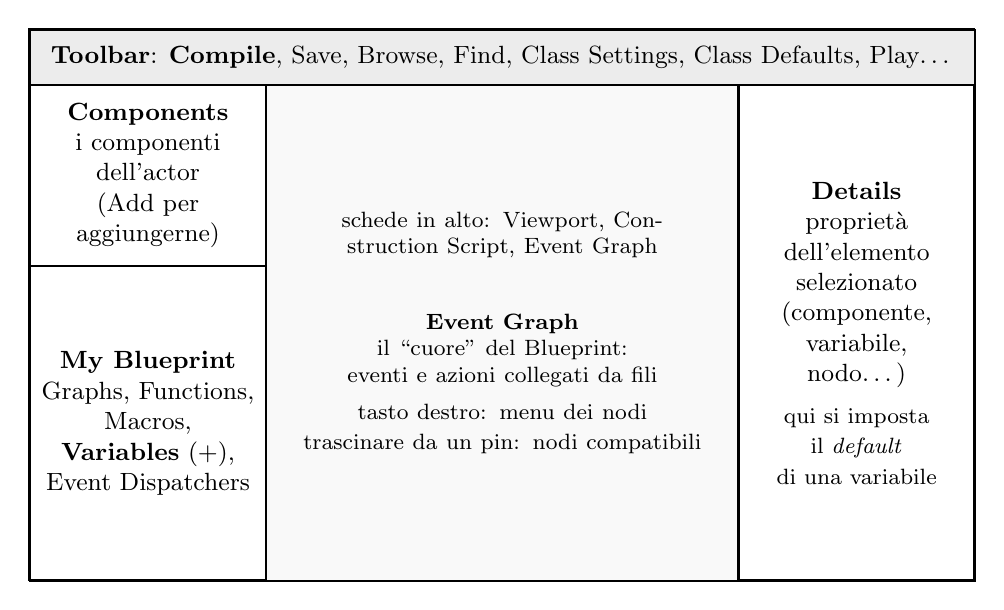
\begin{tikzpicture}[
  font=\small,
  ue2pan/.style={draw, thick, align=center, inner sep=3pt}
]
  \draw[thick] (0,0) rectangle (12,7);
  \node[ue2pan, minimum width=12cm, minimum height=0.7cm, anchor=north west,
    fill=gray!15] at (0,7) {\textbf{Toolbar}: \textbf{Compile}, Save, Browse, Find,
    Class Settings, Class Defaults, Play\ldots};
  \node[ue2pan, minimum width=3cm, minimum height=2.3cm, anchor=north west]
    at (0,6.3) {\textbf{Components}\\i componenti\\dell'actor\\(Add per\\aggiungerne)};
  \node[ue2pan, minimum width=3cm, minimum height=4cm, anchor=north west]
    at (0,4.0) {\textbf{My Blueprint}\\Graphs, Functions,\\Macros,\\
    \textbf{Variables} (+),\\Event Dispatchers};
  \node[ue2pan, minimum width=6cm, minimum height=6.3cm, anchor=north west,
    text width=5.6cm, fill=gray!5] at (3,6.3) {\footnotesize schede in alto:
    Viewport, Construction Script, Event Graph\\[18pt]\textbf{Event Graph}\\il ``cuore'' del Blueprint:\\
    eventi e azioni collegati da fili\\[4pt]\footnotesize tasto destro: menu dei nodi\\
    \footnotesize trascinare da un pin: nodi compatibili};
  \node[ue2pan, minimum width=3cm, minimum height=6.3cm, anchor=north west]
    at (9,6.3) {\textbf{Details}\\proprietà\\dell'elemento\\selezionato\\
    (componente,\\variabile,\\nodo\ldots)\\[4pt]\footnotesize qui si imposta\\
    \footnotesize il \emph{default}\\\footnotesize di una variabile};
\end{tikzpicture}
\caption{L'editor dei Blueprint (Blueprint Class Editor), ricostruito dalla lezione e
dal primo capitolo del libro di Romero e Sewell. La disposizione dei pannelli si può
cambiare, come nel Level Editor.}
\label{ue2:fig:editorbp}
\end{figure}

\paragraph{Approfondimento: i pannelli dell'editor.} Romero e Sewell, nel primo capitolo,
elencano i pannelli principali del \emph{Blueprint Class Editor}: la
\textbf{Toolbar}, i \textbf{Components} (i componenti già pronti che si aggiungono con
Add: \emph{mesh} statiche, luci, suoni, collisioni, particelle, camere), \textbf{My
Blueprint} (dove si creano variabili, macro, funzioni e grafi, con i pulsanti +), i
\textbf{Details} (le proprietà dell'elemento selezionato, con una barra di ricerca in
alto), la \textbf{Viewport} e l'\textbf{Event Graph}. Nell'Event Graph, notano gli
autori, un \textbf{evento} è un nodo \textbf{rosso}, e le altre azioni che seguono un
evento si collegano con dei fili; ci si sposta nel grafo trascinando con il tasto
destro. Di ogni evento se ne può mettere \textbf{uno solo} per grafo, ma si possono
creare eventi propri (\textbf{Add Custom Event}). Oltre a BeginPlay e Tick, il libro
cita gli eventi di \textbf{collisione} (quando due actor si scontrano o si
sovrappongono), gli eventi di \textbf{input} (tastiera, mouse, \emph{touch},
\emph{gamepad}) ed \textbf{Event End Play}, quando l'actor sta per essere rimosso.

% ---------------------------------------------------------------------
\section{Il primo nodo: Print String}
\label{ue2:sec:print}

``Andremo a fare una piccola prova.'' Unreal gestisce tutto con i \textbf{nodi}. Se si
porta il mouse sul ``pinnetto'' bianco a forma di freccia dell'Event BeginPlay, lo si
clicca e lo si \textbf{trascina verso l'esterno}, al rilascio compare un menu con tutti
i blocchi che si possono collegare: ``possiamo metterci tutto quello che vogliamo, tutti
i blocchi che ci serviranno per fare un'azione''.

\paragraph{Print String.} L'azione più semplice è \textbf{Print String}, che
``letteralmente ci stampa qualcosa a schermo''. Il testo predefinito è ``Hello''.

\paragraph{La barra ``Development Only''.} Igor fa notare un dettaglio. A differenza di
altri nodi, come \textbf{Set Actor Location} o \textbf{Enable Collision}, il Print String
ha una \textbf{barra in basso}. Vuol dire che quel blocco ha effetto \textbf{solo in
modalità di sviluppo}: quando si sviluppa e si va in Play nell'editor funziona, ma se si
facesse un \textbf{eseguibile} da mandare a qualcun altro ``questa cosa non avverrà
mai''. Gli altri nodi, invece, sì.

\paragraph{Compilare.} ``Molto importante'': quando si fanno dei cambiamenti
importanti bisogna \textbf{compilare} (\textbf{Compile}, in alto a sinistra). La
compilazione ``legge quello che abbiamo fatto'' e aggiorna il programma; in molti casi
Unreal lo fa anche in automatico, ma conviene farlo sempre. E \textbf{salvare},
``ovviamente, sempre buona cosa''.

\paragraph{La prova.} Si abbassa la finestra del Blueprint, si \textbf{mette l'actor
nella scena} (``ovviamente, se no non succede niente'': il Blueprint è solo una classe,
finché non se ne mette una copia nel livello non esiste) e si preme Play. In alto a
sinistra compare ``Hello'', ma per pochissimo. Igor cambia allora il parametro
\textbf{Duration} del nodo a 100 secondi, e la scritta resta: ``è piccolo'', ma c'è.
L'actor è entrato in funzione e ha fatto la sua azione appena ha cominciato a esistere,
cioè subito, perché era già nella scena.

\paragraph{Una finestra di gioco separata.} ``Se vi è più comodo'', si può far partire il
gioco in una finestra esterna: dai \textbf{tre puntini} accanto al pulsante Play si
sceglie \textbf{New Editor Window (PIE)}. ``Io lo trovo molto più comodo'': invece di
abbassare e rialzare la finestra del Blueprint, il gioco gira in una finestra a parte da
cui si controlla tutto. Igor lo scrive anche in chat.

\paragraph{Approfondimento: \emph{development} e \emph{shipping}.} La barra del Print
String rimanda a una distinzione che Romero e Sewell spiegano nel capitolo sul
\emph{packaging}: le \emph{build} di \textbf{sviluppo} (\emph{Development}) contengono
informazioni che servono al \emph{debug}, quelle di \textbf{distribuzione}
(\emph{Shipping}) sono più ``pulite'', senza informazioni di \emph{debug}, e sono quelle
da pubblicare. I nodi marcati \emph{Development Only}, come il Print String, vengono
semplicemente ignorati in una \emph{build} Shipping: si possono quindi lasciare nel
grafo mentre si lavora senza che il giocatore finale veda mai le scritte di prova.

% ---------------------------------------------------------------------
\section{Le variabili: GET e SET, colori e calcoli}
\label{ue2:sec:variabili}

\paragraph{Che cos'è una variabile.} Igor chiede chi abbia mai sentito parlare di
variabili \emph{bool}, \emph{float}, \emph{int}; qualcuno sì. Una \textbf{variabile} è
``uno slot di una tipologia di valore'' in cui si può mettere un valore: ``è come una
\textbf{scatola}''. Si creano delle piccole scatoline in cui mettere dei valori, ma ogni
scatola è fatta per un certo contenuto: ``c'è la scatola per i gioielli, c'è la scatola
per le praline'' (``mi invento un po' di cose''). Il tipo della variabile decide che cosa
ci si può mettere dentro.

\paragraph{Creare una variabile.} L'esempio: rendere ``esterna'' la durata del Print
String, cioè metterla in una variabile. Nel pannello My Blueprint, alla voce
\textbf{Variables}, si clicca \textbf{+}: si crea subito una variabile, di tipo booleano
oppure dello stesso tipo dell'ultima variabile creata. Igor la chiama \textbf{duration
time text}\footnote{Così nella trascrizione (una volta ``duration time next''); il nome
esatto digitato non si sente, ma non ha importanza per l'esempio.}.

\paragraph{GET e SET.} Se si trascina la variabile nel grafo, Unreal chiede se si vuole
un \textbf{GET} o un \textbf{SET}. GET è \textbf{prendere} il valore che c'è dentro; SET
è \textbf{impostare} il valore dentro. Per dare il valore alla durata del Print String
serve un GET.

\paragraph{I colori devono combaciare.} ``Però attenzione, che succede? Questo è rosso e
questo è verde.'' Il pin della variabile appena creata è \textbf{rosso} (è una
booleana), quello della Duration è \textbf{verde}: ``non sono della stessa tipologia''.
Due pin rossi si collegano; un rosso e un verde no. Il verde è il \textbf{float}. ``Cosa
sono i numeri float?'' ``I numeri con la virgola.'' ``Ottimo'': i numeri con i
\textbf{decimali}. Si cambia quindi il tipo della variabile in Float, il pin diventa
verde, e ``guardate un po', si collega''.

\paragraph{\emph{Please compile the Blueprint}.} Appena collegata, la variabile mostra
l'avviso \emph{please compile the blueprint}: è stata appena creata, e il Blueprint ``non
sa ancora che c'è una variabile nuova''. Dopo la compilazione, nei Details compare il
suo \textbf{valore predefinito} (\emph{Default Value}): ``guarda, questo è il tuo valore.
Quanto lo vuoi?'' Igor mette 10. In Play la scritta dura 10 secondi (``un po' tanti'') e
poi scompare: ``non è più 100''. La lezione: si possono creare variabili, impostarle e
darle ai blocchi di esecuzione.

\paragraph{Nodi di esecuzione e nodi di calcolo.} I \textbf{blocchi di esecuzione} si
riconoscono perché hanno l'intestazione \textbf{blu} e il pin di esecuzione, ``la
freccettina'' bianca. Ci sono però anche nodi \textbf{verdi} senza quel pin: sono nodi
che ``\textbf{calcolano solamente}''. Igor ne fa vedere uno, \textbf{Find Look at
Rotation}: chiede due variabili di un tipo e ne restituisce un'altra, dello stesso tipo
o di un altro. ``Oppure, esempio classico'': gli \textbf{operatori} aritmetici, il
\textbf{+}, il \textbf{$-$} (\emph{Subtraction}), il \textbf{per}, che si cerca con
l'\textbf{asterisco} (\emph{Multiply}), e il \textbf{diviso} (\emph{Divide}). Si
possono invocare tutti gli operatori che servono (figura~\ref{ue2:fig:pin}).

\paragraph{Sottrarre due secondi.} L'esempio: ``indipendentemente da quanto tempo noi
mettiamo qua dentro'', togliere sempre 2 secondi. Si prende il nodo meno, si collega la
variabile al primo ingresso (il nodo ``è diventato verde'', perché ha riconosciuto che si
tratta di un float, e ``ci chiede: te lo sottraggo di un altro float''), si scrive 2 nel
secondo e si collega il risultato alla Duration.

\paragraph{Da numero a testo.} Si può anche \textbf{stampare} il valore: collegando il
float all'ingresso di testo del Print String, Unreal inserisce in automatico un
\textbf{convertitore}. I pin \textbf{rosa} sono le \textbf{stringhe}, cioè testo. In
Play, il Print String non stampa più ``Hello'' ma \textbf{8}, ``che è 10 meno 2'', e la
scritta dura 8 secondi. (Ogni volta che Igor apre Unreal, Zoom va a scatti: ``a quanto
pare mi lagga Zoom benissimo''.)

\begin{figure}[htbp]
\centering
\begin{tikzpicture}[
  font=\small,
  ue2node/.style={draw, thick, rounded corners=4pt, align=center},
  ue2exec/.style={-{Stealth[length=2.5mm]}, very thick},
  ue2flt/.style={-{Stealth[length=2mm]}, thick, green!50!black},
  ue2str/.style={-{Stealth[length=2mm]}, thick, magenta}
]
  \node[ue2node, fill=red!15, minimum width=2.6cm, minimum height=1.2cm]
    (bp) at (0,0) {\textbf{Event}\\\textbf{BeginPlay}};
  \node[ue2node, fill=blue!10, minimum width=3.4cm, minimum height=2.6cm,
    anchor=north west] (pr) at (7.4,0.6) {};
  \node[font=\small\bfseries, anchor=north] at (pr.north) {Print String};
  \node[font=\footnotesize, anchor=west] (ins) at (7.5,-0.5) {In String};
  \node[font=\footnotesize, anchor=west] (dur) at (7.5,-1.2) {Duration};
  \node[font=\scriptsize\itshape, anchor=south] at (pr.south) {Development Only};
  \node[ue2node, fill=green!10, minimum height=0.8cm] (get) at (0.4,-1.9)
    {GET duration (float)};
  \node[ue2node, fill=green!10, minimum height=0.8cm] (minus) at (3.6,-1.9)
    {$x - 2$};
  \node[ue2node, fill=magenta!8, minimum height=0.8cm, font=\footnotesize]
    (conv) at (5.6,-0.5) {float $\to$ string};
  \draw[ue2exec] (bp.east) -- node[above, font=\footnotesize]{esecuzione}
    (bp.east -| pr.west);
  \draw[ue2flt] (get) -- (minus);
  \draw[ue2flt] (minus.east) -- ++(0.4,0) |- (dur.west);
  \draw[ue2flt] (minus.north) |- (conv.west);
  \draw[ue2str] (conv.east) -- (ins.west);
\end{tikzpicture}
\caption{Il primo grafo della lezione, nella sua versione finale: all'inizio del gioco
l'actor stampa la durata meno 2 (cioè 8) per 8 secondi. La freccia nera è il filo di
\textbf{esecuzione} (l'ordine delle azioni, da sinistra a destra); le frecce colorate
sono fili di \textbf{dati}, del colore del loro tipo (verde il float, rosa la stringa).
Il nodo blu, con il pin di esecuzione, è un'\textbf{azione}; i nodi verdi, senza, sono
nodi di \textbf{calcolo}, che si eseguono quando un'azione chiede il loro valore. Il
convertitore è inserito da Unreal in automatico. Schema ricostruito, non copia della
schermata.}
\label{ue2:fig:pin}
\end{figure}

% ---------------------------------------------------------------------
\section{Primo esercizio: Time To Print}
\label{ue2:sec:esercizio1}

``Vorrei fare un piccolo esercizio con voi. Molto velocissimo.''

\paragraph{Staccare un filo.} Prima, un comando: per \textbf{staccare} un collegamento
si tiene premuto \textbf{Alt} e si clicca sul pin.

\paragraph{La consegna.} Creare un'altra variabile, \textbf{time to print}, di tipo
\textbf{float}; staccare la variabile della durata dall'ingresso del testo e collegarci
invece time to print; dare a time to print il valore \textbf{5}, che dovrà essere
stampato a schermo. Anche la Duration va messa a 5. ``Senza che andiamo a vedere poi
ognuno'': l'importante è che ognuno dica ``stampa 5, sì''.

\paragraph{Un esercizio guidato.} Uno studente arriva in ritardo (``scusate, non
riuscivo ad entrare''). A una studentessa il Print String stampa \textbf{0}, e Igor la
guida passo per passo in condivisione dello schermo: fermare il gioco (lo
\textbf{Stop}, o il tasto \textbf{Esc}); creare la variabile dal \textbf{+} di Variables
nel pannello a sinistra; chiamarla time to print; cambiarle il tipo per farla
\textbf{verde}, cioè float (``bravissima''); prenderne il GET; staccare il vecchio
collegamento con Alt e attaccare time to print; compilare (``in alto a sinistra'');
poi, con la variabile selezionata, guardare nei \textbf{Details} a destra: ``vedi, adesso
è apparsa. In fondo''. In fondo ai Details c'è il \textbf{valore predefinito}, ed è lì
che si mette il 5. Lo 0 dipendeva proprio da questo: il valore predefinito di un float
appena creato è zero.

% ---------------------------------------------------------------------
\section{I dettagli di una variabile, e il \emph{tuning}}
\label{ue2:sec:dettagli}

Tutte le caratteristiche di una variabile si vedono nei \textbf{Details}, sia cliccando
la variabile nel grafo, sia cliccandola nella lista Variables. Igor consiglia di
impostare l'engine \textbf{in inglese} (``io sono più abituato all'inglese''), ma se si
trova più facile l'italiano non c'è nessun problema.

\paragraph{Il nome, il tipo, la descrizione.} Nei Details si possono cambiare il nome, il
tipo e una \textbf{descrizione}. La descrizione non la vedrà il giocatore, ma ``i nostri
amici programmatori, o comunque colleghi'': ci si può scrivere un piccolo commento,
come ``variabile da stampare nel Print''. È un'informazione ``per lo più organizzativa'',
``non un qualcosa che troverete spesso''.

\paragraph{Pubblica e privata: Instance Editable.} L'opzione \textbf{Instance Editable}
rende una variabile \textbf{pubblica}. Gli studenti non conoscono la distinzione ``in
questo contesto''. Una variabile \textbf{privata} esiste solo all'interno dell'actor;
una \textbf{pubblica} si può vedere e modificare direttamente nei \textbf{Details}
dell'actor piazzato nel livello. Uno studente chiede se sia come ``globale e locale''.
``Non esattamente, perché globale è anche un'altra cosa che andremo a vedere'': le
variabili davvero globali si fanno con la \textbf{Game Instance}, un oggetto che
\textbf{esiste finché esiste il gioco} e che può contenere variabili da ``dare in pasto''
a tutti gli actor che si vuole.

\paragraph{L'occhietto.} Lo stesso risultato si ottiene con l'icona
dell'\textbf{occhio} accanto alla variabile nella lista. Igor lo mostra: con l'occhio
aperto, selezionando l'actor nel livello, nei Details compare la sezione
\textbf{Default} con \emph{time to print}; con l'occhio chiuso, dopo aver ricompilato,
la voce scompare.

\paragraph{Il \emph{tuning}.} A che cosa serve? ``Il design è sempre con me.'' Come
designer, a Igor è capitato spesso di fare \textbf{\emph{tuning}}: la pratica di
\textbf{aggiustare i valori}, ``quanto danno fa, quanto fa di contrattacco'', in
generale i valori modificabili. Diceva al programmatore: ``lasciami quei valori, che li
devo controllare'', cioè testare. E poi andava nei Details dell'actor e cambiava
``questo, quell'altro, questo, quell'altro''. Le variabili pubbliche servono proprio a
questo: permettono di \textbf{interagire con l'editor stesso} senza toccare il grafo. Le
cose private, invece, restano nel campo dell'actor.

\paragraph{Approfondimento: gli attributi di una variabile.} Romero e Sewell, nel secondo
capitolo, elencano tutti gli attributi che i Details mostrano per una variabile.
\begin{itemize}
  \item \textbf{Variable Name} e \textbf{Variable Type}: il nome e il tipo. I Blueprint
        sono un linguaggio \textbf{fortemente tipizzato}: il tipo si sceglie alla
        creazione e non cambia durante l'esecuzione.
  \item \textbf{Instance Editable}: se attivo, \textbf{ogni copia} del Blueprint
        piazzata nel livello può avere un valore diverso; altrimenti tutte le copie
        (le \emph{istanze}) condividono lo stesso valore iniziale. È la precisazione
        tecnica del ``pubblico'' di Igor.
  \item \textbf{Blueprint Read Only}: se attivo, i nodi non possono modificare la
        variabile.
  \item \textbf{Tooltip}: il testo che compare passando il mouse sulla variabile; è la
        ``descrizione'' di cui parla Igor.
  \item \textbf{Expose on Spawn}: la variabile si può impostare nel momento in cui
        l'actor viene \emph{spawnato}.
  \item \textbf{Private}: se attivo, i Blueprint figli non possono modificarla.
  \item \textbf{Expose to Cinematics}: la rende visibile al Sequencer.
  \item \textbf{Category}: per raggruppare le variabili.
  \item \textbf{Slider Range} e \textbf{Value Range}: il minimo e il massimo, per lo
        \emph{slider} e per i valori ammessi. Per il \emph{tuning} sono preziosi: chi
        aggiusta i valori non può uscire dai limiti sensati.
  \item \textbf{Replication}: per i giochi in rete.
  \item \textbf{Default Value}: il valore iniziale; si può impostare solo dopo aver
        compilato, come si è visto nell'esercizio.
\end{itemize}

% ---------------------------------------------------------------------
\section{I tipi di variabile}
\label{ue2:sec:tipi}

Igor cancella tutto (seleziona e preme \textbf{Canc}, \emph{Delete} sulla tastiera
inglese) e passa a una slide sui tipi di variabile (tabella~\ref{ue2:tab:tipi}).
``Immaginiamoci sempre delle scatolette, con dentro dei valori.''

\paragraph{Booleana.} ``Qualcuno ha mai sentito parlare di booleane?'' Qualche sì,
qualche no. Una variabile \textbf{booleana} ha due valori possibili: \textbf{vero} o
\textbf{falso}. ``Dentro o c'è vero, o c'è falso, una delle due. Basta.'' Con un esempio
dall'elettrotecnica, è ``letteralmente lo \emph{switch} della luce'': spento è falso,
acceso è vero; a livello di circuito, ``è aperto o è chiuso''.

\paragraph{Byte, Integer, Integer64.} Il \textbf{byte} è un valore numerico intero
compreso tra 0 e 255. L'\textbf{integer}\footnote{Nella trascrizione ``gli integrali, i
numeri integrali''.}, o intero, è un numero \textbf{senza la virgola}: ``1, 2, 3, 4, 5,
6, 7, 8, senza virgola, senza niente'', compreso tra $-2^{31}$ e $2^{31}$ (``possiamo
anche non capire qual è il numero preciso, perché tanto è difficile che ci arriviamo'').
L'\textbf{integer64} arriva a 64 bit, tra $-2^{63}$ e $2^{63}$.

\paragraph{Float.} Il \textbf{float} è il valore numerico \textbf{con i decimali}.

\paragraph{Name, String, Text.} Il \textbf{name} è un testo usato principalmente per gli
\textbf{identificatori}, per identificare degli elementi in Unreal. La \textbf{string}
è un gruppo di caratteri \textbf{alfanumerici}, ``numeri e lettere''. Uno studente chiede
la differenza: anche il name è una stringa? La stringa, risponde Igor, si usa per lo più
nei \textbf{testi}; i name sono \textbf{nomenclature}: ``il nome di un livello, il nome
di un \emph{asset}''. ``Tipo un'etichetta'', propone lo studente: ``bravissimo, è come
un'etichetta'', ``quasi come un \textbf{tag}''. Il \textbf{text}, infine, è un testo
usato principalmente nella \textbf{UI}, la \emph{user interface}: tutto ciò che è 2D e
con cui l'utente interagisce, un termine usato ``in tanti campi, anche coi siti''.

\paragraph{Vector, Rotator, Transform.} I \textbf{vettori} sono ``molto importanti'',
essendo Unreal un ambiente tridimensionale. Un vettore può essere la
\textbf{locazione}: ``ci ricordiamo che quando abbiamo spostato i nostri cubetti e coni
abbiamo visto quei tre valori cambiare, la X, la Y e la Z?'' Un vettore è ``la
composizione'' di questi tre: una variabile che contiene \textbf{tre valori}, X, Y e Z.
Il \textbf{rotator} contiene gli X, Y e Z della \textbf{rotazione} (``poi faremo un po'
di discorsi, perché esistono i quaternioni, eccetera''). Il \textbf{transform}
contiene location, rotation e scala.

\paragraph{Object.} Infine il tipo \textbf{object}: ``volendo, noi potremmo creare una
variabile di tipologia di un actor che abbiamo creato''. È una variabile che contiene un
\textbf{riferimento} a un actor (si vedrà con il Level Blueprint,
sezione~\ref{ue2:sec:level}).

\begin{table}[htbp]
\centering
\small
\begin{tabular}{@{}p{2.2cm}p{2.0cm}p{8.8cm}@{}}
\toprule
\textbf{Tipo} & \textbf{Colore} & \textbf{Che cosa contiene} \\
\midrule
Boolean & rosso & vero o falso (\emph{true}/\emph{false}) \\
Byte & verde scuro & intero da 0 a 255 (8 bit) \\
Integer & verde acqua & intero da $-2^{31}$ a $2^{31}-1$ (32 bit) \\
Integer64 & verde acqua scuro & intero da $-2^{63}$ a $2^{63}-1$ (64 bit) \\
Float & verde & numero con decimali; in Unreal Engine 5 i Blueprint lo trattano in
  precisione singola o doppia (\emph{Double}) \\
Name & lilla & identificatore, ``etichetta'' (nome di un livello, di un \emph{asset}) \\
String & rosa & gruppo di caratteri alfanumerici \\
Text & rosa scuro & testo per la UI, \textbf{localizzabile} (traducibile) \\
Vector & giallo & tre float X, Y, Z (per esempio una locazione) \\
Rotator & viola-lilla & tre float della rotazione: X (\emph{roll}), Y (\emph{pitch}),
  Z (\emph{yaw}) \\
Transform & arancione & locazione, rotazione e scala \\
Object & blu & riferimento a un oggetto (per esempio un actor nel livello) \\
\bottomrule
\end{tabular}
\caption{I tipi di variabile della slide di Igor, con i colori dei loro pin
nell'editor (i nomi dei colori sono approssimativi) e le integrazioni del libro di
Romero e Sewell (i limiti esatti degli interi, \emph{roll}, \emph{pitch} e \emph{yaw},
la localizzazione del Text).}
\label{ue2:tab:tipi}
\end{table}

\paragraph{Approfondimento: Double, Text e i tre angoli.} Tre precisazioni dal secondo
capitolo del libro. Primo: oltre al Float a 32 bit (sette cifre decimali di
precisione) esiste il \textbf{Double} a 64 bit (sedici cifre); in Unreal Engine 5 l'editor
mostra entrambi come ``Float'' e sceglie la precisione da solo. Secondo: il
\textbf{Text} serve ai testi che saranno \textbf{localizzati}, cioè tradotti in altre
lingue: è per questo che è il tipo della UI, mentre String è il testo ``di servizio'' e
Name l'identificatore. Terzo: i tre valori del \textbf{Rotator} hanno un nome. X è il
\textbf{\emph{roll}} (il rollio, la rotazione attorno all'asse X, quello ``in avanti''),
Y il \textbf{\emph{pitch}} (il beccheggio, attorno all'asse Y, alzare o abbassare il
muso), Z lo \textbf{\emph{yaw}} (l'imbardata, attorno all'asse Z verticale, girare a
destra e a sinistra). Sono i nomi che compariranno nei nodi della piattaforma
(sezione~\ref{ue2:sec:mouse}). I \textbf{quaternioni} a cui accenna Igor sono un altro
modo, matematicamente più robusto, di rappresentare una rotazione: evitano il problema
del \emph{gimbal lock}, in cui due dei tre assi finiscono per coincidere e si perde un
grado di libertà. Unreal li usa al suo interno, ma nei Blueprint si lavora quasi sempre
con i Rotator.

% ---------------------------------------------------------------------
\section{Le booleane e il Branch}
\label{ue2:sec:branch}

``Adesso vi faccio vedere.'' Igor crea una variabile, la chiama ``letteralmente''
\textbf{bool}, e le dà il tipo booleano.

\paragraph{GET e SET in un gesto.} ``Piccola cosetta'': invece di scegliere dal menu, si
può fare un GET ``velocissimamente'' trascinando la variabile nel grafo con
\textbf{Ctrl} premuto, e un SET trascinandola con \textbf{Alt}. Il \textbf{GET} è il pin
che dice ``questa è la scatoletta che c'è dentro qualcosa, prendi il valore da qui''. Il
\textbf{SET} è diverso: ha un \textbf{nodo di esecuzione}, a differenza del GET, e ha una
\textbf{casella di spunta}\footnote{Nella trascrizione ``un TIL'': è il \emph{tick},
la spunta della casella.}: cliccandola si imposta il valore. ``Col SET sto letteralmente
impostando il suo valore'': spunta, vero; niente spunta, falso.

\paragraph{Stampare una booleana.} Igor rifà un Print String con Duration 10 (``sennò è
troppo poco''), collega il pin della booleana al testo e va in Play: in alto a sinistra
compare \textbf{false}. Mette la spunta, rifà Play: \textbf{true}. Il Print String
riceve, tramite la stringa, il valore della variabile.

\paragraph{A che cosa serve sapere se è vero o falso?} ``La domanda magari è: ok, ma che ci
serve?'' Serve perché si possono usare delle \textbf{condizioni}. ``Qualcuno ha mai
sentito parlare di \emph{if}, \emph{else}?'' Edoardo sì: ``ho studiato informatica alle
superiori''. ``Grande, perfetto.'' L'\textbf{if-else} è una condizione, e in Unreal non si
chiama così: tenendo premuto \textbf{B} e cliccando nel grafo compare il
\textbf{Branch}, ``cioè due percorsi''. È ``un \textbf{bivio}'': ``se questa condizione
che abbiamo qua è vera, vai per questo percorso; se questa condizione è falsa, vammi per
un altro''.

\paragraph{Il primo Branch.} Igor collega il Branch dopo il BeginPlay e porta la
variabile bool nel pin rosso \textbf{Condition}. Sull'uscita \textbf{True} mette un Print
String con ``la variabile è vera''; per l'uscita \textbf{False} copia il nodo (``per
copiare qualcosa, Ctrl+C, Ctrl+V, classico'') e scrive ``la variabile è falsa''. Con la
variabile falsa, in Play esce ``la variabile è falsa''; con la spunta, ``la variabile è
vera'' (figura~\ref{ue2:fig:branch}).

\paragraph{I binari del treno.} ``Letteralmente sta prendendo un bivio: o vado di qua, o
vado di là.'' Igor lo paragona ai \textbf{binari di un treno}: ``se la leva è a destra,
vado a destra; se la leva è a sinistra, vado a sinistra. E la nostra leva è la nostra
variabile''. Il bool è molto importante perché permette di avere delle condizioni, e
quindi gli attori ``\textbf{pensano}'': hanno la ``capacità di scelte'', ``ah, ok, allora
prendo questa strada perché ho questa variabile di questo tipo''.

\begin{figure}[htbp]
\centering
\begin{tikzpicture}[
  font=\small,
  ue2node/.style={draw, thick, rounded corners=4pt, align=center,
                  minimum height=1cm},
  ue2exec/.style={-{Stealth[length=2.5mm]}, very thick},
  ue2bool/.style={-{Stealth[length=2mm]}, thick, red!70!black}
]
  \node[ue2node, fill=red!15, minimum width=2.4cm] (bp) at (0,0)
    {\textbf{Event}\\\textbf{BeginPlay}};
  \node[ue2node, fill=gray!10, minimum width=2.2cm, minimum height=1.6cm]
    (br) at (4,0) {\textbf{Branch}\\[2pt]\footnotesize Condition};
  \node[ue2node, fill=green!8, minimum width=1.6cm] (get) at (1.6,-1.8) {GET bool};
  \node[ue2node, fill=blue!10, text width=3.6cm] (pt) at (9,0.9)
    {\textbf{Print String}\\\footnotesize ``la variabile è vera''};
  \node[ue2node, fill=blue!10, text width=3.6cm] (pf) at (9,-0.9)
    {\textbf{Print String}\\\footnotesize ``la variabile è falsa''};
  \draw[ue2exec] (bp) -- (br);
  \draw[ue2bool] (get.east) -| ([xshift=-4mm]br.south);
  \draw[ue2exec] ([yshift=4mm]br.east) -- node[above, font=\footnotesize]{True}
    ++(1.2,0) |- (pt.west);
  \draw[ue2exec] ([yshift=-4mm]br.east) -- node[below, font=\footnotesize]{False}
    ++(1.2,0) |- (pf.west);
\end{tikzpicture}
\caption{Il Branch è un bivio: segue l'uscita True o l'uscita False a seconda del valore
della condizione. ``La nostra leva è la nostra variabile.''}
\label{ue2:fig:branch}
\end{figure}

\paragraph{Si può accedere al codice?} Uno studente chiede se sia possibile accedere anche
al codice, ``immagino che sia C''. Sì, è possibile, ``però non lo faremo''. Con il C++ si
possono definire anche i blocchi stessi, creare blocchi di tipo diverso; ma ``di base, su
Blueprint possiamo farlo allo stesso modo anche noi''. Chi vuole può andare a vederlo; e
c'è chi va ``proprio nel profondo della programmazione'', come gli \emph{engine
programmer}.

\paragraph{Allineare i nodi.} ``Una piccola cosa, se vi piace l'ordine'': si selezionano
due nodi e si preme \textbf{Q}, e Unreal li allinea.

\paragraph{Approfondimento: Branch e operatori relazionali.} Romero e Sewell presentano il
Branch nel secondo capitolo, parlando del \textbf{percorso di esecuzione}: i pin bianchi
sono i \textbf{pin di esecuzione}, gli altri, colorati, i \textbf{pin di dati};
l'esecuzione parte da un evento rosso e segue il filo bianco da sinistra a destra fino
all'ultimo nodo. Alcuni nodi, come il Branch, \textbf{controllano il flusso}: decidono
quale strada prendere. Il loro esempio è un personaggio con una booleana \emph{Has
Shield}: se è vera, il Branch imposta \emph{Shield Value} a 100; se è falsa, a 0. Nella
lezione la condizione è sempre una variabile booleana; nella pratica, spesso, è il
risultato di un \textbf{operatore relazionale}: i nodi $<$, $\leq$, $>$, $\geq$, $=$,
$\neq$ confrontano due valori e restituiscono una booleana. L'esempio del libro: quando
un oggetto subisce danni, un Branch controlla se \emph{Health} $\leq 0$, e in quel caso
l'oggetto viene distrutto; se no, non succede niente, perché all'uscita False non è
collegato nulla. Quanto alla scorciatoia: nel menu che si apre con il tasto destro su
una selezione di nodi c'è la voce \textbf{Alignment}, con allineamenti in alto, al
centro, in basso, a sinistra, a destra, e \textbf{Straighten Connection(s)}, che
raddrizza i fili; il tasto \textbf{Q} è la scorciatoia di quest'ultima. Il libro ricorda
anche le altre scorciatoie ``tasto + clic'': \textbf{B} per il Branch, \textbf{S} per il
nodo Sequence, \textbf{D} per il Delay, \textbf{F} per il For Each Loop
(tabella~\ref{ue2:tab:scorciatoie}).

% ---------------------------------------------------------------------
\section{Gli operatori logici: AND, OR, NOT}
\label{ue2:sec:logici}

Igor cancella i nodi di prova (``tanto non ci sono problemi'') e passa agli
\textbf{operatori logici}. ``Qualcuno ha mai sentito parlare di AND, OR, NOT?'' Sì.

\paragraph{Il gioco dei tubi.} A che cosa servono? Una variabile booleana ha i suoi valori,
vero e falso; ``però mettiamo conto che ne abbiamo altre'', e bisogna metterle in
\textbf{comparazione}. L'esempio è ``il gioco dei tubi'', l'enigma in cui bisogna girare i
tubi nel verso giusto per collegarli. Se ci sono due tubi, per risolvere l'enigma un tubo
deve essere girato nel modo giusto \textbf{e} anche l'altro: sono \textbf{due
condizioni} da prendere insieme. ``Come facciamo a metterle insieme?''

\paragraph{I nodi.} Igor crea una seconda booleana, \textbf{bool 2}. Gli operatori si
cercano scrivendo \textbf{OR Boolean}, \textbf{AND Boolean} e \textbf{NOT Boolean}.
``Questi sono i tre più usati''; ce ne sono altri, come il NOR, ``ma sono un attimo da
vedere poi più avanti''.

\paragraph{OR.} L'OR dice: ``se almeno un valore è vero, allora la condizione finale è
vera''. Con bool vera e bool 2 falsa, collegato alla condizione del Branch, esce ``la
variabile è vera''. È ``un modo per sommare le variabili tra \emph{true} e \emph{false}'',
``una specie di somma, chiamiamola così'': ``letteralmente dice: o questa, o questa''.

\paragraph{AND.} L'AND, con gli stessi valori, vero e falso, dà ``la variabile è falsa'',
``perché AND vuol dire \emph{questa e questa}'': tutte le condizioni devono essere vere
perché il risultato sia vero. Igor mette vera anche la seconda e\ldots{} non succede
niente: ``scusate, questo non l'ho collegato, sono io''. Collegato, esce ``la variabile è
vera''. Ricapitolando: se tutte e due sono vere, è vero; se una sola è falsa, ``tutto
quanto è falso''; se tutte e due sono false, è falso (``doppio falso'').

\paragraph{NOT.} Il NOT ha un solo ingresso e ``letteralmente \textbf{inverte}'': se la
variabile è vera diventa falsa, se è falsa diventa vera. Collegato a una variabile vera,
dà falso. ``Non lo useremo tanto.'' La tabella~\ref{ue2:tab:logici} riassume i tre
operatori.

\begin{table}[htbp]
\centering
\small
\begin{tabular}{@{}cc|ccc|ccc@{}}
\toprule
\textbf{A} & \textbf{B} & \textbf{A OR B} & \textbf{A AND B} & \textbf{NOT A} &
  \textbf{A NOR B} & \textbf{A NAND B} & \textbf{A XOR B} \\
\midrule
falso & falso & falso & falso & vero  & vero  & vero  & falso \\
falso & vero  & vero  & falso & vero  & falso & vero  & vero  \\
vero  & falso & vero  & falso & falso & falso & vero  & vero  \\
vero  & vero  & vero  & vero  & falso & falso & falso & falso \\
\bottomrule
\end{tabular}
\caption{Le tabelle di verità degli operatori logici. Le prime tre colonne di risultati
sono gli operatori della lezione; le ultime tre sono un'integrazione dal libro di Romero
e Sewell.}
\label{ue2:tab:logici}
\end{table}

\paragraph{Approfondimento: NOR, NAND, XOR, e perché l'OR è una ``somma''.} Il libro
completa la lista degli operatori logici dei Blueprint con tre combinazioni. Il
\textbf{NOR} (NOT + OR) è vero solo se entrambi gli ingressi sono falsi; il \textbf{NAND}
(NOT + AND) è falso solo se entrambi sono veri; lo \textbf{XOR}, l'OR esclusivo, è vero
se i due ingressi sono \textbf{diversi}. L'esempio del libro per l'AND: un Print String
che si esegue solo se \emph{Health} $> 70$ \textbf{e} \emph{Shield Value} $> 50$, con
due operatori relazionali che alimentano un AND. Quanto alla ``somma'' di Igor, è
un'intuizione che ha un nome: nell'\textbf{algebra di Boole}, da cui il tipo
\emph{boolean} prende il nome, l'OR si scrive come una somma ($A + B$) e l'AND come un
prodotto ($A \cdot B$). Se si leggono vero e falso come 1 e 0, l'AND si comporta
esattamente come una moltiplicazione (basta uno 0 per fare 0), e l'OR come una somma
in cui ``1 + 1'' resta 1.

% ---------------------------------------------------------------------
\section{Secondo esercizio: due Branch, OR e AND}
\label{ue2:sec:esercizio2}

``Allora facciamo un piccolo esercizio.''

\paragraph{La consegna.} All'Event BeginPlay si collega un \textbf{SET} della variabile
bool (quello che si ottiene trascinandola con Alt), e il suo valore va alla condizione
di un \textbf{primo Branch}. Su ciascuna uscita del primo Branch va un \textbf{secondo
Branch}: su True un Branch la cui condizione è \textbf{bool OR bool 2}; su False un
Branch la cui condizione è \textbf{bool AND bool 2}. Solo se il secondo Branch è vero si
stampa, e invece di ``la variabile è vera'' si stampa \textbf{il valore finale} del
calcolo, collegando l'uscita dell'operatore all'In String
(figura~\ref{ue2:fig:esercizio2}). ``Ce la fate?'' Cinque minuti.

\begin{figure}[htbp]
\centering
\begin{tikzpicture}[
  font=\small,
  ue2node/.style={draw, thick, rounded corners=4pt, align=center,
                  minimum height=0.9cm},
  ue2exec/.style={-{Stealth[length=2.5mm]}, very thick},
  ue2bool/.style={-{Stealth[length=2mm]}, thick, red!70!black}
]
  \node[ue2node, fill=red!15] (bp) at (0,0) {\textbf{BeginPlay}};
  \node[ue2node, fill=blue!10] (set) at (2.6,0) {\textbf{SET bool}\\\footnotesize
    $\square$ / $\checkmark$};
  \node[ue2node, fill=gray!10] (b1) at (5.2,0) {\textbf{Branch 1}\\\footnotesize
    cond.\ = bool};
  \node[ue2node, fill=gray!10] (b2) at (8.4,1.5) {\textbf{Branch 2}};
  \node[ue2node, fill=gray!10] (b3) at (8.4,-1.5) {\textbf{Branch 3}};
  \node[ue2node, fill=green!8] (or) at (8.4,3.1) {bool \textbf{OR} bool 2};
  \node[ue2node, fill=green!8] (and) at (8.4,-3.1) {bool \textbf{AND} bool 2};
  \node[ue2node, fill=blue!10, text width=2.3cm] (p1) at (11.6,1.5)
    {\textbf{Print}\\\footnotesize risultato OR};
  \node[ue2node, fill=blue!10, text width=2.3cm] (p2) at (11.6,-1.5)
    {\textbf{Print}\\\footnotesize risultato AND};
  \draw[ue2exec] (bp) -- (set);
  \draw[ue2exec] (set) -- (b1);
  \draw[ue2exec] (b1.east) ++(0,0.2) -- ++(0.5,0) |- node[pos=0.75, above,
    font=\footnotesize]{True} (b2.west);
  \draw[ue2exec] (b1.east) ++(0,-0.2) -- ++(0.5,0) |- node[pos=0.75, below,
    font=\footnotesize]{False} (b3.west);
  \draw[ue2bool] (or) -- (b2);
  \draw[ue2bool] (and) -- (b3);
  \draw[ue2exec] (b2) -- node[above, font=\footnotesize]{True} (p1);
  \draw[ue2exec] (b3) -- node[below, font=\footnotesize]{True} (p2);
  \draw[ue2bool, dashed] (or.east) -| (p1.north);
  \draw[ue2bool, dashed] (and.east) -| (p2.south);
\end{tikzpicture}
\caption{Il secondo esercizio. Le frecce nere sono l'esecuzione, quelle rosse i valori
booleani (tratteggiate: il risultato dell'operatore, convertito in testo e stampato). Le
uscite False dei Branch 2 e 3 non sono collegate: in quei casi non si stampa niente.}
\label{ue2:fig:esercizio2}
\end{figure}

\paragraph{Le domande durante l'esercizio.} Lo studente arrivato in ritardo chiede come
si crea il Print String: tasto destro, Print String. Un altro si è perso gli operatori:
si scrivono proprio ``AND Boolean'', ``OR Boolean'', ``NOT Boolean''. Una studentessa non
ricorda come si prende ``l'oggetto con il pallino rosso'' (la variabile): ``mettilo qua
dentro, ti appare in automatico''. Trascinando la variabile direttamente sul pin, Unreal
crea da solo il GET.

\paragraph{La spunta che non c'entra.} Un'altra studentessa ha un problema: sul primo
Branch, nella condizione, ha una \textbf{spunta} che Igor non ha. Il pin Condition non è
collegato all'\textbf{uscita} del SET. ``Devi collegare questo pallino a questo
pallino.'' Igor spiega che cosa è successo, con una dimostrazione. Il nodo SET ha a
destra un pin di uscita: ``è il valore che io gli ho impostato'', che esce dal nodo
``come un collegamento''. Il Branch ha a sinistra ``un posto in cui posso mettere quel
valore''. Se il pin non è collegato, la casella di spunta del Branch è una
\textbf{condizione interna al Branch}, che non ha niente a che vedere con la variabile:
``la porta si aprirà secondo bool, non secondo questa condizione qua''. Igor mette la
variabile a vero e la spunta del Branch a falso: il Print String collegato al True
``non mi stampa niente'', ``perché questa qua non è relativa a questa''. Collegando il
pin, stampa. (``Stavo impazzendo perché non mi stampava niente.'')

\paragraph{I ``what if''.} Poi Igor cerca ``un candidato'' per una piccola verifica:
``se io adesso vi cambio un po' i parametri, dove andiamo a finire con tutte le linee?''
Si offre uno studente.
\begin{itemize}
  \item \textbf{bool vero, bool 2 falso.} ``Siccome è \emph{true}, finisce sopra, sul
        primo Branch'' (il Branch 2 della figura). ``Controlla se tra bool e bool 2 uno
        dei due è vero. In questo caso lo è, perché hai settato bool come vero. Il
        secondo non è importante.'' Quindi va su True e stampa il valore. ``Perfetto.
        Netto, liscio.''
  \item \textbf{bool falso.} ``False scende giù e controlla se entrambi, bool e bool 2,
        sono veri. In questo caso bool è falso, quindi anche qui il secondo valore non
        è importante, perché uno dei due è falso. Il risultato dell'AND è falso e non
        stampa niente.'' ``Esatto, perfetto.''
\end{itemize}
La morale: ``indipendentemente dalle condizioni, possiamo cambiare i binari di un
percorso di programmazione''. È ``una delle cose più principali'', e serve molto spesso
per \textbf{diversificare i comportamenti} dei Blueprint. Igor chiede ancora se ci sono
domande, e decide di non cancellare il grafo ma di lasciarlo lì, scollegato. ``Sono stato
chiaro, dai.''

\paragraph{Approfondimento: la valutazione ``pigra''.} Lo studente coglie, senza
nominarlo, un principio importante: in un OR, se il primo ingresso è vero il secondo
``non è importante''; in un AND, se il primo è falso il secondo non cambia il risultato.
In molti linguaggi di programmazione questo si chiama \emph{short-circuit evaluation}
(valutazione a corto circuito): il secondo operando non viene nemmeno calcolato. Nei
nodi Blueprint, attenzione, i due ingressi vengono comunque calcolati entrambi; ma il
ragionamento sul \emph{risultato} è lo stesso, ed è quello che serve per prevedere dove
andrà l'esecuzione.

% ---------------------------------------------------------------------
\section{Il Level Blueprint e la piattaforma}
\label{ue2:sec:level}

``Adesso andremo a fare una piccola cosa direttamente nel nostro bellissimo Blueprint.''
L'obiettivo è una \textbf{piattaforma} che \textbf{ruota}, cioè si inclina, ``a seconda
di quanto premiamo'' dei tasti (D, A, e così via).

\paragraph{La piattaforma.} Si prende un \textbf{cubo} dal pannello Place Actors, lo si
mette in scena e lo si allarga ``quanto volete'', fino a farne una piattaforma.

\paragraph{Il Level Blueprint.} ``Vi farò conoscere il bellissimo mondo del \textbf{Level
Blueprint}.'' In Unreal esiste anche un Blueprint \textbf{interno al livello}: quando si
apre quel livello, al suo interno ci sono delle regole (``spawna qualcosa'', eccetera).
Lo si apre dall'icona dei Blueprint nella barra in alto: \textbf{Open Level Blueprint}.
Una studentessa si è persa (``scusa, come lo apriamo?''), e Igor le mostra l'icona.

\paragraph{Un evento di input.} Si è parlato di eventi con le loro condizioni; uno dei più
semplici è l'\textbf{input}. Tasto destro nel grafo, si scrive \textbf{W} e si sceglie
la voce con ``l'immaginetta della tastierina'' e la W: è un evento che scatta
\textbf{alla pressione del tasto W}.

\paragraph{La referenza.} Ma come si dice al grafo che deve agire su \emph{quella}
piattaforma? Si crea una \textbf{referenza}. Con il cubo selezionato nel livello, nel
Level Blueprint si fa tasto destro e si sceglie \textbf{Create a Reference to Cube94}
(il cubo di Igor si chiama Cube94, e lo si ritrova con quel nome nell'Outliner). ``Questo
può essere fatto solo nel Level Blueprint, ve lo dico.''

\paragraph{Set Actor Rotation e i suoi pin.} Dalla referenza si trascina un filo e si
sceglie \textbf{Set Actor Rotation}. Il nodo ha tre pin di dati:
\begin{itemize}
  \item un pin \textbf{blu}, il \textbf{Target}: un \emph{Actor Object Reference}, cioè
        una variabile che si riferisce a un actor, a uno qualunque degli elementi della
        \emph{viewport}, ``che abbiano programmazione o meno''. È l'actor su cui il nodo
        agisce;
  \item un pin \textbf{lilla}, \textbf{New Rotation}: un \textbf{rotator}, la
        composizione degli assi X, Y e Z della rotazione;
  \item un pin \textbf{rosso}, un \textbf{bool}: \textbf{Teleport} (tornerà utile con
        la fisica, sezione~\ref{ue2:sec:fisica}).
\end{itemize}

\paragraph{Il Player Start.} Per vedere la piattaforma serve un punto da cui partire.
``Prendete il \textbf{Player Start}'': lo si trova nel Place Actors, o cercandolo, ed è
``un controllone'' (l'icona di un \emph{joystick}). Lo si mette davanti alla piattaforma
e lo si gira verso di essa.

\paragraph{Consume Input.} Selezionando l'evento W, nei Details c'è una casella
interessante, \textbf{Consume Input}. Se è spuntata, il tasto W ``sarà dedicato solo a
questo evento'': il giocatore non potrà più usarlo per muoversi in avanti. Senza la spunta
si muoverebbe ``avanti e indietro''; ``a noi interessa stare fermi'', quindi la spunta
resta.

\paragraph{Quale asse, e in che verso.} La piattaforma va ruotata attorno all'asse
\textbf{X}. In positivo o in negativo? Igor lo verifica nella \emph{viewport} ruotando il
cubo: in un verso la rotazione è negativa, nell'altro positiva. ``Per come mi regolo'',
W manda la piattaforma in avanti, quindi si piega in un verso, e indietro nell'altro.
Igor scrive 5 nella X del New Rotation e prova.

% ---------------------------------------------------------------------
\section{La mobilità: Static, Stationary, Movable}
\label{ue2:sec:mobilita}

Non funziona, ``giustamente'', e Unreal mostra un avviso: ``ricordate che questo che mi è
appena uscito è un problema che Unreal ci darà sempre''. L'actor non ha la capacità di
essere \textbf{Movable}: non si può muovere nel mondo.

\paragraph{Dove si trova.} Nel \emph{transform} dell'actor, sotto location, rotation e
scala, c'è la \textbf{Mobility}, con tre valori: \textbf{Static}, \textbf{Stationary} e
\textbf{Movable}. È ``la tipologia di oggetto'' rispetto a come reagisce al mondo, e
riguarda ``soprattutto il rendering''.
\begin{itemize}
  \item \textbf{Static.} L'oggetto sa che non si muoverà. Quando si calcolano le luci,
        la sua ombra viene calcolata una volta e poi è come \textbf{dipinta}: ``è
        dipinta''. ``Per alleggerirsi la cosa'', l'engine dice: è un oggetto statico,
        ``basta che mi calcolo una volta l'ombra e basta''.
  \item \textbf{Stationary.} Una via di mezzo: le ombre vengono messe in
        \emph{cache}\footnote{Nella trascrizione ``vengono chesciate'': con ogni
        probabilità ``cachate'', dall'inglese \emph{cached}.}, l'oggetto può essere
        cambiato, ma non può essere mosso.
  \item \textbf{Movable.} Totalmente \textbf{dinamico}.
\end{itemize}
La piattaforma va messa su \textbf{Movable}, e allora ruota di 5 gradi. Igor prova con
valori più grandi (``facciamo tipo 25'') per vederlo meglio.

\paragraph{Approfondimento: la mobilità secondo il libro.} Romero e Sewell incontrano lo
stesso problema nel quinto capitolo, quando un bersaglio cilindrico deve cominciare a
muoversi: bisogna prima portare la sua Mobility da Static a \textbf{Movable}, nei Details
sotto il TRANSFORM. E aggiungono una nota importante: gli actor di base piazzati nel
mondo sono \textbf{Static per impostazione predefinita}, e gli oggetti statici sono
``significativamente meno costosi'' da renderizzare; per questo Static dovrebbe essere
la scelta predefinita per tutto ciò che non è interattivo, per tenere alto il
\emph{frame rate}. Stationary ha senso soprattutto per le \textbf{luci}: una luce
Stationary non si sposta, ma se ne possono cambiare colore e intensità durante il gioco,
e parte della sua illuminazione è precalcolata. Movable va riservato agli oggetti che
devono davvero muoversi.

% ---------------------------------------------------------------------
\section{Ruotare di 5 gradi a ogni pressione: Split Struct Pin}
\label{ue2:sec:split}

\paragraph{Funziona una volta sola.} ``Però che succede? Guardate un po'.'' Se si preme
di nuovo W, la piattaforma non fa niente. Il problema è che la si sta impostando a un
\textbf{valore preciso}: Set Actor Rotation dice ``mettiti a 25 gradi'', e la seconda
volta la piattaforma risponde ``ci sto già, a 25''. Serve invece una rotazione che
\textbf{parta da quella attuale}.

\paragraph{Prendere i valori dell'actor.} Igor mostra che dalla referenza di un actor si
possono prendere \textbf{tutti} i suoi valori: la location, la rotation, la scala, la
\emph{mesh}, i materiali (``che poi vedremo''). ``È andare nella scatola di
quell'\emph{asset}'': prendo quel valore, e poi lo modifico. Qui serve \textbf{Get Actor
Rotation}, la rotazione attuale, ``che si aggiorna ogni volta''.

\paragraph{Split Struct Pin.} La rotazione è data da tre valori, X, Y e Z, e se ne vuole
modificare uno solo. Con il tasto destro sul pin del Rotator si sceglie \textbf{Split
Struct Pin}: il pin si divide nei suoi tre valori, ``e guardate un po', la cosa bella è
che sono cambiati di colore''. Sono diventati \textbf{verdi}, ``perché sono tre valori
float''. Uno studente chiede come si fa a trovare i tre valori; Igor rifà il gesto
all'indietro (\textbf{Recombine Struct Pin}) e poi di nuovo avanti: tasto destro, Split
Struct Pin. Si fa lo stesso sul pin New Rotation del Set Actor Rotation, che altrimenti,
lilla, non accetterebbe un float.

\paragraph{Il grafo.} Si prende la X di Get Actor Rotation, le si somma 5 con un nodo
\textbf{+}, e il risultato va nella X del Set Actor Rotation
(figura~\ref{ue2:fig:piattaforma}, a sinistra). Ora la piattaforma si inclina di 5 gradi
a ogni pressione di W: ``posso aggiungere quanto me ne pare'', a parte che a un certo
punto la piattaforma \textbf{compenetra} il pavimento. ``Prima non andava bene e adesso
invece sì'', perché ogni volta si parte dalla rotazione attuale. Con un Print String
collegato alla X, a ogni pressione compaiono i valori \textbf{0, 5, 10, 15, 20, 25, 30,
35}: ``si aumenta sempre''.

\begin{figure}[htbp]
\centering
\begin{tikzpicture}[
  font=\small,
  ue2node/.style={draw, thick, rounded corners=4pt, align=center,
                  minimum height=0.9cm},
  ue2exec/.style={-{Stealth[length=2.5mm]}, very thick},
  ue2flt/.style={-{Stealth[length=2mm]}, thick, green!50!black},
  ue2obj/.style={-{Stealth[length=2mm]}, thick, blue!70!black}
]
  % versione prima della pausa
  \node[font=\footnotesize\bfseries] at (2.6,2.2) {Prima della pausa};
  \node[ue2node, fill=red!15] (w) at (0,1.2) {\textbf{W}\\\footnotesize Pressed};
  \node[ue2node, fill=blue!10, text width=3.2cm] (set) at (4.6,1.2)
    {\textbf{Set Actor Rotation}\\\footnotesize New Rotation (split)};
  \node[ue2node, fill=blue!5] (ref) at (0,-0.6) {Cube94};
  \node[ue2node, fill=green!8, text width=2.0cm] (get) at (2.0,-1.9)
    {\textbf{Get Actor Rotation}\\\footnotesize (split)};
  \node[ue2node, fill=green!8] (plus) at (4.6,-0.6) {X $+\,5$};
  \draw[ue2exec] (w) -- (set);
  \draw[ue2obj] (ref.east) -- ++(0.4,0) |- (get.west);
  \draw[ue2obj] (ref.north) -- ++(0,0.3) -| ([xshift=-12mm]set.south);
  \draw[ue2flt] (get.east) -| (plus.south);
  \draw[ue2flt] (plus) -- (set);
  % separatore
  \draw[gray, dashed] (7.2,2.4) -- (7.2,-2.6);
  % versione dopo la pausa
  \node[font=\footnotesize\bfseries] at (10.2,2.2) {Dopo la pausa};
  \node[ue2node, fill=red!15] (w2) at (8.4,1.2) {\textbf{W}};
  \node[ue2node, fill=blue!10, text width=3.2cm] (add) at (11.8,1.2)
    {\textbf{Add Actor World}\\\textbf{Rotation}\\\footnotesize Delta Rotation: X $= 5$};
  \node[ue2node, fill=blue!5] (ref2) at (8.4,-0.6) {Cube94};
  \node[ue2node, fill=red!15] (s2) at (8.4,-1.9) {\textbf{S}};
  \node[ue2node, fill=blue!10, text width=3.2cm] (add2) at (11.8,-1.6)
    {\textbf{Add Actor World}\\\textbf{Rotation}\\\footnotesize X $= -5$};
  \draw[ue2exec] (w2) -- (add);
  \draw[ue2exec] (s2) -- (add2);
  \draw[ue2obj] (ref2.east) -- ++(0.5,0) |- ([yshift=-2mm]add.west);
  \draw[ue2obj] (ref2.east) -- ++(0.5,0) |- ([yshift=2mm]add2.west);
\end{tikzpicture}
\caption{La piattaforma comandata da tastiera, nel Level Blueprint. A sinistra la prima
versione: si legge la rotazione attuale, si aggiungono 5 gradi alla X e la si reimposta.
A destra la versione adottata dopo la pausa: Add Actor World Rotation aggiunge
direttamente 5 gradi (o $-5$) alla rotazione, nello spazio del mondo. A e D funzionano
allo stesso modo sull'asse Y.}
\label{ue2:fig:piattaforma}
\end{figure}

% ---------------------------------------------------------------------
\section{Il problema di Giulia, e la pausa}
\label{ue2:sec:problema}

``Un attimo, un attimo.'' A Giulia la piattaforma si muove \textbf{una volta sola}. Igor
segue il problema in condivisione dello schermo, e il \emph{debug} dal vivo è istruttivo anche
perché non arriva a una risposta.
\begin{itemize}
  \item La piattaforma è \textbf{Movable}? Sì.
  \item Il grafo è uguale a quello di Igor? Sembra di sì: Cube71 (il suo cubo), Set
        Actor Rotation, il più, il Get Actor Rotation. Ruotata a mano con E nella
        \emph{viewport}, la piattaforma ruota normalmente.
  \item Forse un problema di \textbf{collisioni} con il pavimento? Igor fa alzare la
        piattaforma: niente.
  \item Igor fa rifare alcuni collegamenti, ricostruire il nodo, splittarlo di nuovo,
        eliminare un nodo superfluo (``questo get actor\ldots{} l'actor location
        sopra?'', ``è uguale, lo elimino''), ricollegare il Target al Cube71. Niente.
  \item La \textbf{camera}: Giulia vede ``la piattaforma sbilenca e basta''. Igor fa
        girare il Player Start di 90 gradi e mettere la piattaforma davanti. Niente.
  \item Ha cliccato nella finestra di gioco, perché riceva l'input? Sì, ``solo una
        volta''. Il Consume Input c'è.
  \item Un controllo più fine: Igor chiede di selezionare il nodo Set Actor Rotation e
        premere \textbf{F9}, che vi mette un \emph{breakpoint}. In Play il nodo viene
        effettivamente raggiunto: ``funziona a meraviglia''. Eppure la piattaforma non
        ruota oltre la prima volta.
  \item Infine Giulia si accorge che nel livello \textbf{manca il Player Start}
        (``mancano delle robe che ho cercato di mettere, ma ho perso''). Igor fa
        rimettere il Player Start dal Place Actors.
\end{itemize}
A quel punto è ora della pausa: ``facciamo pausa, io intanto cerco di capire un po' il
problema che c'è, Giulia''. Venti minuti.

\paragraph{La soluzione, durante la pausa.} Durante la pausa Igor prova una cosa diversa:
al posto di Set Actor Rotation, con il Get e il più, usa \textbf{Add Actor World
Rotation}, con la referenza come Target e 5 nella X (``senza il più, senza niente, solo
questi due''; $-5$ per la S, che Giulia non ha ancora). ``Sì, adesso lo fa. Perfetto.''
``Ma era un errore mio?'' ``No, no, tranquillo.'' La spiegazione di Igor è che il problema
dipende dagli assi: con Set Actor Rotation si stava ruotando ``sulla sua relativa'', ed è
meglio ruotare sull'asse \textbf{globale}, quello del mondo. Ma su un punto Igor è
onesto: ``il fatto che non prenda l'input a ogni W, quello non te lo so dire, perché a
tutti quanti lo prendeva''. ``Non so se magari è un \emph{flash} o un qualcosa, non ne ho
idea. Ti devo dire la verità.'' Per capirlo dovrebbe guardare con calma le impostazioni
dell'editor di Giulia; intanto si semplifica. ``Visto che ho risolto la cosa, vado a farmi il
caffè'', dice Giulia. ``Ottima idea. Pure io.''

\paragraph{Approfondimento: Set, Add Local, Add World, e il \emph{breakpoint}.} Unreal ha
più nodi per ruotare un actor, e la differenza è esattamente quella tra assi locali e
globali vista nella prima lezione.
\begin{itemize}
  \item \textbf{Set Actor Rotation} imposta una rotazione \textbf{assoluta}: ``mettiti
        così''. Per ottenere un incremento bisogna leggere la rotazione attuale e
        sommarci qualcosa, come nella prima versione.
  \item \textbf{Add Actor Local Rotation} aggiunge una rotazione attorno agli assi
        \textbf{locali} dell'actor, quelli che ruotano con lui.
  \item \textbf{Add Actor World Rotation} aggiunge una rotazione attorno agli assi
        \textbf{del mondo}, che restano fissi: premere W inclina sempre la piattaforma
        ``in avanti'' rispetto alla scena, comunque sia già inclinata.
\end{itemize}
Perché la prima versione non funzionasse sul computer di Giulia la lezione non lo
stabilisce, e il capitolo non è in grado di dirlo; il passaggio sul nodo ``get actor
location'' da eliminare fa pensare a un collegamento sbagliato (la \emph{location},
gialla, al posto della \emph{rotation}, lilla), ma è solo un'ipotesi. Resta istruttivo
il metodo. Il \textbf{\emph{breakpoint}} (F9 su un nodo selezionato) ferma l'esecuzione
quando il gioco arriva a quel nodo e apre l'editor del Blueprint lì, mostrando i valori
che passano nei fili: è il modo più diretto per sapere se un nodo viene davvero eseguito
e con quali dati. Lo stesso F9 lo toglie. Il Print String, che Igor usa per tutta la
lezione, è l'altro strumento: stampa i valori a schermo senza fermare il gioco.

% ---------------------------------------------------------------------
\section{Dopo la pausa: Add Actor World Rotation e i tasti W A S D}
\label{ue2:sec:wasd}

``Ora ci siamo, ragazzi?'' Visto il problema di Giulia, Igor semplifica l'esercizio per
tutti, con il blocco che ha usato durante la pausa: \textbf{Add Actor World Rotation},
``nel senso che andiamo semplicemente a mettere una rotazione nel mondo, non dipendente
dalla sua relatività''. Prima, spiega, si impostava la rotazione relativa all'asse
dell'actor; doveva essere relativa al mondo. La consegna: tenere solo i due blocchi
(l'evento e Add Actor World Rotation), levare tutto il resto, \textbf{splittare} il pin
della rotazione e scrivere 5 nella X (figura~\ref{ue2:fig:piattaforma}, a destra).
``Praticamente qui si dovrebbe tranquillamente muovere, molto più semplice.''

\paragraph{S, A e D.} Igor ha aggiunto anche la \textbf{S}: ``se una è 5, l'altra è
$-5$''. E per destra e sinistra, A e D? ``Su che asse ci dobbiamo muovere?'' Lo si vede
nella \emph{viewport}: cliccando la piattaforma e guardando il gizmo, se W e S ruotano
attorno alla X, A e D devono ruotare attorno alla \textbf{Y}. ``E vorrei questo piccolo
esercizio: lo fate voi.'' A e D, ``non è Donkey Kong, questo con la tastiera''. ``Mi
raccomando, ricordatevi sempre che il \textbf{Target} è importante'': senza collegarlo, il
nodo non si riferisce a niente.

\paragraph{Allineare in verticale?} Uno studente chiede se esista un tasto per allineare i
blocchi in verticale. ``Non lo conosco, devo dire la verità.'' (L'allineamento c'è, nel
menu Alignment del tasto destro: si veda l'approfondimento della
sezione~\ref{ue2:sec:branch}.)

\paragraph{Qual è il verso di D?} Un altro studente non capisce che valore mettere sulla
D. Igor lo guarda insieme a lui sulla piattaforma: destra, nella sua vista, è ``di là'',
opposto a lui. Ruotando a mano la piattaforma in quel verso, il valore che compare sulla
Y è negativo: ``siccome siamo in asse globale, devi andare in negativo sulla Y''. La
soluzione, ``velocissimamente, perché se no non abbiamo tempo'': gli stessi due blocchi,
il Target collegato, la rotazione sulla Y, $+5$ per un tasto e $-5$ per l'altro. ``E
possiamo, wow, destra e sinistra.''

% ---------------------------------------------------------------------
\section{La pallina, la fisica e il Teleport}
\label{ue2:sec:fisica}

``Qua sopra, una bella sferetta.'' In Unreal gli oggetti possono essere
\textbf{fisici}. Si prende una \textbf{sfera} dal Place Actors e la si mette sulla
piattaforma. In Play, però, ``quella rimane lì, sta lì ferma'': ``non gliene frega
assolutamente nulla''. La sua fisica non è attiva.

\paragraph{Simulate Physics.} Nei Details della sfera c'è la casella \textbf{Simulate
Physics}. Spuntata, in Play la sfera \textbf{cade} e rotola: ``abbiamo la nostra sferetta
che si muove''. Uno studente chiede dove si attiva: basta cliccare la sfera e cercare la
voce. Un altro condivide lo schermo: ``una cosa che va, finalmente''.

\paragraph{La pallina scagliata.} C'è però una cosa particolare: muovendo la
piattaforma, la sfera viene \textbf{scagliata in alto}, oltre a uscire dai bordi. Che
esca si risolve ``semplicemente mettendoci un muro, un muro invisibile'' (lo si farà alla
fine, sezione~\ref{ue2:sec:vaschetta}). Che venga lanciata, invece, dipende dal modo in
cui la piattaforma si muove.

\paragraph{La freccia sotto il nodo, e il Teleport.} Nel Level Blueprint, sotto il nodo
Add Actor World Rotation c'è una \textbf{freccia}: cliccandola si aprono altri parametri.
``Molto spesso blocchi del genere hanno queste tipologie di parametri interni, che sono
nascosti un po'.'' Uno è \textbf{Teleport}. La spiegazione di Igor: quando c'è uno
spostamento nello spazio, l'engine lo fa avvenire sui \emph{tick}, sui \emph{frame}, e
``pum!'': lo spostamento porta con sé il \textbf{fattore fisico}, ``abbiamo proprio là il
colpo fisico'', che spinge via la pallina. Se invece lo si \textbf{teletrasporta}, ``è
come fare un \emph{pop-up}'' dello spostamento della piattaforma: l'effetto fisico si
annulla, e la pallina non viene scaricata via. Igor abbassa un po' la pallina, spunta
Teleport su tutti i nodi e va in Play: ``la nostra palletta non verrà influenzata dalla
particolarità fisica della nostra piattaforma''.

\paragraph{Approfondimento: che cosa fa davvero Teleport.} Quando Unreal sposta o ruota
un oggetto che partecipa alla simulazione fisica, deve decidere come trattare quel
movimento. Con \textbf{Teleport} disattivato, lo spostamento è considerato un movimento
``vero'': il motore fisico ricava dalla differenza tra la posizione vecchia e quella
nuova una \textbf{velocità}, e la trasmette agli oggetti a contatto. Una piattaforma che
ruota di 5 gradi in un solo \emph{frame} ha, per il motore fisico, una velocità enorme,
e la pallina riceve un colpo proporzionato. Con \textbf{Teleport} attivo, lo spostamento
è un salto istantaneo, senza velocità associata: la pallina si ritrova sulla piattaforma
nella nuova posizione e scivola per gravità, senza essere colpita. Accanto a Teleport,
nella stessa sezione nascosta, c'è spesso \textbf{Sweep}: se attivo, l'oggetto si ferma
quando nel tragitto incontra qualcosa che lo blocca, invece di attraversarlo.

\paragraph{I bug della fisica.} Mentre gli studenti provano, uno trova ``un \emph{bug}'':
se si porta la pallina in un angolo e si premono insieme W e A, cioè le direzioni
opposte all'angolo, la pallina \textbf{finisce sotto} la piattaforma. (Un altro nota che
E porta il giocatore in alto e Q in basso: anche durante il gioco ci si muove come
nell'editor.) Igor risponde che ``possono esserci dei \emph{bug} fisici'', perché la
\textbf{fisica è emergente}: spostare le cose con la fisica dipende da come la si
gestisce, e ``probabilmente ne potresti trovare non pochi''. Ci sono engine proprietari,
``come quello di Valve'', che gestiscono fisica e gravità ``in un modo assurdo'', ``con
molto matematichese'', e sono ottimizzati per le azioni che quei giochi fanno. Unreal,
``essendo più generico come sistema fisico'', può dare problemi fisici ``molto più
evidenti, molto più spesso''.

\paragraph{``Non va niente''.} Uno studente ha messo anche la S, ma premendo W, A, S, D
non succede niente. Igor gli fa cliccare la piattaforma: non è \textbf{Movable}. ``È la
terza'' delle tre opzioni. Rimessa su Movable, funziona; manca solo il Teleport.

\paragraph{Approfondimento: il motore fisico di Unreal.} Unreal Engine 5 usa un motore
fisico proprio, \textbf{Chaos}, che ha sostituito PhysX della quarta versione. È pensato
per essere generale: corpi rigidi, distruzione, tessuti, veicoli. Il caso della pallina
che finisce sotto la piattaforma ha un nome, \textbf{\emph{tunneling}}: se in un
\emph{frame} un oggetto si sposta più dello spessore di ciò che dovrebbe fermarlo, il
motore fisico non vede mai il contatto e l'oggetto ``passa attraverso''. Con il Teleport
attivo la piattaforma salta da una rotazione all'altra senza che la fisica la segua, e
il rischio aumenta. Le difese tipiche sono oggetti più spessi, spostamenti più piccoli a
ogni \emph{frame} e la \textbf{CCD} (\emph{Continuous Collision Detection}), un'opzione
dei componenti fisici che controlla le collisioni lungo tutto il tragitto e non solo
nelle posizioni finali.

% ---------------------------------------------------------------------
\section{L'Event Tick e i \emph{delta seconds}}
\label{ue2:sec:tick}

``Abbiamo il nostro bellissimo gioco della palla incredibile.'' Il passo successivo è
comandare la piattaforma con il \textbf{mouse} invece che con W A S D. Prima, però, un
evento nuovo.

\paragraph{Che cos'è un tick.} ``Sapete cos'è un \emph{tick}?'' È, semplicemente,
``\textbf{un per \emph{frame}}''. L'\textbf{Event Tick} è un blocco che esegue tutto ciò
che c'è dopo di lui \textbf{a ogni \emph{frame}}: ``ogni \emph{tick}, ogni \emph{tick},
ogni \emph{frame}''.

\paragraph{La piattaforma che gira da sola.} Igor copia un Add Actor World Rotation,
collega la referenza come sempre e lo attacca all'Event Tick: 5 gradi a ogni
\emph{frame}. ``Non sto premendo nulla'', e la piattaforma gira da sola, velocissima.
Quanti sono gli \emph{fps}? ``In questo caso saranno tipo 100'': la piattaforma ruota di 5
gradi cento volte al secondo.

\paragraph{I \emph{delta seconds}.} L'Event Tick ha un'uscita, \textbf{Delta Seconds}:
``l'intervallo tra un \emph{frame} e l'altro''. Perché la velocità sia la stessa
``indipendentemente dal numero di \emph{frame}'' (30, 60, 70, 100), bisogna
\textbf{moltiplicare} il valore per i \emph{delta seconds}. Si tira fuori un
\textbf{Multiply}, si collega Delta Seconds e si scrive 5. ``Vedete, è molto diverso da
prima'': la piattaforma gira molto più piano. Prima si aggiungevano 5 gradi a ogni
\emph{frame}; ora si moltiplica il tempo tra i \emph{frame} per 5. E se il gioco
girasse a 30, 60, 70, 100, 120 o 144 \emph{fps}, la velocità sarebbe la stessa; senza la
moltiplicazione, con un limite a 30 \emph{fps} sarebbe più lenta che a 100.

\paragraph{``Un tick ogni 5 frame?''} Uno studente prova a riformulare: ``quindi in realtà
non fa partire il programma ogni 5 \emph{tick}, ma fa in modo che un \emph{tick} sia ogni
5 \emph{frame}?'' ``Non 5 \emph{frame}: 5 \textbf{unità}'', le unità in cui si muove la
piattaforma; ``è il float, fondamentalmente''. Il \emph{tick} resta uno per
\emph{frame}; cambia quanto si muove l'oggetto a ogni \emph{tick}.

\paragraph{La regola.} ``Questa è una cosa da tenere tanto a mente, soprattutto con
oggetti che si muovono.'' Se in un progetto si fa un oggetto in movimento senza
\emph{delta seconds}, ``vi si ritorcerà contro'': su una macchina con certe prestazioni
andrà più lento, su un'altra più veloce. ``Moltiplicatevi i \emph{delta seconds} se
muovete le cose, soprattutto nel tempo.'' Per il gioco della pallina, però, la rotazione
continua non serve, ``perché se no non ha \emph{gameplay}'': ``sarebbe quasi un
mulino''.

\paragraph{Approfondimento: i conti.} Con i numeri di Igor: senza \emph{delta seconds},
5 gradi per \emph{frame} a 100 \emph{fps} fanno $5 \times 100 = 500$ gradi al secondo,
quasi un giro e mezzo; a 30 \emph{fps} ne fanno 150. Con i \emph{delta seconds}, a 100
\emph{fps} ($\Delta t = 0{,}01$~s) ogni \emph{frame} aggiunge $5 \times 0{,}01 = 0{,}05$
gradi, a 30 \emph{fps} ($\Delta t \approx 0{,}033$~s) circa $0{,}167$: in un secondo, in
entrambi i casi,
\[
  \sum_{\text{frame in 1 s}} 5 \cdot \Delta t = 5 \cdot 1~\text{s} = 5~\text{gradi}.
\]
Il 5, insomma, non è più ``gradi per \emph{frame}'' ma \textbf{gradi al secondo}: è la
``unità'' di cui parla Igor rispondendo allo studente. Romero e Sewell, nel secondo
capitolo, descrivono l'Event Tick proprio così (a 60 \emph{frame} al secondo viene
chiamato 60 volte al secondo) e, nel quinto, usano lo stesso prodotto velocità $\times$
\emph{delta time} per muovere un bersaglio. Più avanti, presentando i
\textbf{timer}, il libro li indica come alternativa all'Event Tick: tutto ciò che si
collega al Tick viene eseguito a ogni \emph{frame}, e ciò che non ha bisogno di
aggiornarsi così spesso può essere eseguito a intervalli più lunghi.

% ---------------------------------------------------------------------
\section{La piattaforma comandata dal mouse}
\label{ue2:sec:mouse}

``Adesso sto staccando tutto, stacco tutto quanto. Voglio dare il movimento al mio
mouse.''

\paragraph{Evento o valore.} Per il mouse ci sono due cose diverse con lo stesso nome.
C'è l'\textbf{evento} \textbf{Mouse X}, che scatta ``quando ho un input dal mouse X'', e
c'è il \textbf{valore} \textbf{Get Mouse X}, ``proprio il valore del mouse X''. Mouse X
è il movimento del mouse a destra e a sinistra (Mouse Y, in alto e in basso). Invece di
usare un evento, Igor fa ``molto più semplice'': resta sull'Event Tick, collega
\textbf{Get Mouse X} al \textbf{Roll} (la X della rotazione) e \textbf{Get Mouse Y} al
\textbf{Pitch} (la Y) dell'Add Actor World Rotation. La piattaforma si muove con il
mouse; ``è molto incontrollabile'', ma si muove.

\paragraph{Assi scambiati, e invertiti.} I due valori risultano scambiati, ``perché
dipende dalla \emph{world location}'', da come è orientata la piattaforma rispetto al
mondo: si invertono X e Y, ``ed è molto meglio''. Poi c'è il verso. A Igor non piace
che, portando il mouse in giù, la piattaforma si pieghi in quel modo: ``lo vogliamo fare
al contrario''. ``Qualcuno ha qualche idea per invertire un valore? In matematica, come
si inverte un valore in negativo?'' ``Moltiplichi per meno 1.'' ``Bravissimo.'' Si prende
Get Mouse X, si aggiunge un \textbf{Multiply} per $-1$, ``in modo tale che farà
l'inverso''. (Più tardi Igor aggiunge che chi preferisce i controlli invertiti, ``se vi
piace di più'', può tranquillamente togliere il $-1$.)

\paragraph{Che cosa si è visto finora.} ``Quindi oggi abbiamo visto praticamente come si
fanno'' le operazioni: crearsi dei valori, moltiplicarli, metterli e poi assegnarli, in
questo caso alla rotazione; volendo, si potrebbero assegnare anche nuove locazioni.
Igor pensa per un momento di far muovere la pallina con un \textbf{Add Torque} (``no,
quella è sempre rotazione''), e decide invece di migliorare la piattaforma: per ora la si
può ruotare ``quanto mi pare'', anche capovolgerla.

\paragraph{Il Clamp.} ``Voglio spiegarvi uno degli operatori che ci permettono di
controllare i nostri valori'': il \textbf{Clamp} (``non Clamp Axis, scusate''; il nodo
giusto è \textbf{Clamp (Float)}). Igor prova a disegnare su Zoom con uno strumento di
annotazione, ``ma a quanto pare non funziona'' (``sarà per la prossima volta''), e lo
spiega a voce: \textbf{clampare} un valore vuol dire dargli \textbf{un minimo e un
massimo}, in modo che ``viaggi su queste due linee'' e non le superi mai. Igor mette un
Clamp su entrambi gli assi, tra $-1$ e $1$: il movimento diventa ``più preciso''.

\paragraph{``Perché valori così piccoli?''} Una studentessa chiede perché proprio $-1$ e 1:
lei aveva messo $-45$ e 45, ``pensando ai gradi della rotazione''. ``Ah, i gradi! No.''
Si possono modificare a piacere, ma 45 ``è un po' troppo''. In quel punto del grafo,
infatti, il Clamp non limita l'inclinazione: limita \textbf{quanto} la piattaforma può
ruotare a ogni \emph{frame}.

\paragraph{La versione con il limite d'inclinazione.} ``Allora, ragazzi, adesso abbiamo
questo, ma non abbiamo finito.'' L'obiettivo vero è che la piattaforma non si inclini
oltre un certo angolo. Il grafo (figura~\ref{ue2:fig:mouse}) diventa:
\begin{enumerate}
  \item dalla referenza del cubo, \textbf{Get Actor Rotation}, la rotazione attuale;
  \item invece dello Split Struct Pin, ``una cosa carina che magari vi può servire'':
        un nodo \textbf{Break Rotator}, ``la stessa cosa di fare lo split'', che divide
        il Rotator nei suoi tre valori;
  \item si \textbf{somma} il valore del mouse all'asse corrispondente della rotazione
        attuale (la Y, per Get Mouse X): ``lo stesso discorso di prima: prendere la
        sua rotazione e sommargliela con quella del mouse, in modo che si aggiorni
        continuamente'';
  \item la somma passa per un \textbf{Clamp} tra $-20$ e $20$: ``abbiamo clampato il
        valore, ma vogliamo che vada massimo a 20 o a $-20$'';
  \item un \textbf{Make Rotator} ricompone una rotazione nuova con i valori clampati;
  \item un \textbf{Set Actor Rotation}, con il Target collegato e \textbf{Teleport
        Physics} attivo, ``perché è lo stesso discorso'' della pallina. Qui si torna a
        Set Actor Rotation, invece di Add Actor World Rotation, perché la rotazione
        nuova è già calcolata per intero.
\end{enumerate}

\paragraph{La costruzione dal vivo.} Costruire questo grafo in diretta non è lineare, e
la trascrizione lo mostra. Igor a un certo punto pensa di moltiplicare anche qui per i
\emph{delta seconds}\footnote{Il passaggio è quasi incomprensibile nella trascrizione
(``facciamo così, che mi crea\ldots{} i secondi e la moltiplichiamo per'') e Igor
toglie subito dopo il Clamp precedente; dalla ricapitolazione finale risulta che nel
grafo definitivo i \emph{delta seconds} non ci sono.}, poi toglie il Clamp tra $-1$ e
1, rompe i collegamenti, ne rifà altri, si accorge di un problema di inversione (``ah,
c'è proprio un problema sull'inversione'', ``infatti, sospettavo''), e per capirlo
stampa i valori. Alla fine la soluzione è la stessa di prima: \textbf{invertire X e
Y}. ``Perdonate, colpa mia.'' Con due Print String, uno per asse, si vede in alto a
sinistra che il valore arriva a $-20$ ``e rimane lì, fermo''; lo stesso a 20, su
entrambi gli assi. La piattaforma ``si piega solamente così''.

\paragraph{La ricapitolazione.} ``Dopo tutto sto baradam di roba'', che cosa si è fatto?
Si prende Get Mouse Y (e Get Mouse X) e lo si \textbf{aggiunge continuamente alla
rotazione attuale}: ``adesso è 5, adesso è 7, adesso è 8, adesso è 9, adesso è 10'', e
si aggiunge sempre qualcosa, finché la somma non arriva a 20 o a $-20$. Lì il Clamp la
ferma. ``Stessa identica cosa vale per tutte e due le assi.''

\begin{figure}[htbp]
\centering
\begin{tikzpicture}[
  font=\small,
  ue2node/.style={draw, thick, rounded corners=4pt, align=center,
                  minimum height=0.9cm},
  ue2exec/.style={-{Stealth[length=2.5mm]}, very thick},
  ue2flt/.style={-{Stealth[length=2mm]}, thick, green!50!black},
  ue2rot/.style={-{Stealth[length=2mm]}, thick, violet}
]
  \node[ue2node, fill=red!15] (tick) at (0,1.6) {\textbf{Event Tick}};
  \node[ue2node, fill=green!8, text width=2.1cm] (gar) at (0,0)
    {\textbf{Get Actor}\\\textbf{Rotation}\\\footnotesize (Cube)};
  \node[ue2node, fill=green!8, text width=1.6cm] (brk) at (2.7,0)
    {\textbf{Break}\\\textbf{Rotator}};
  \node[ue2node, fill=green!8, text width=2.3cm] (mx) at (2.5,-1.9)
    {Get Mouse X\\\footnotesize ($\times -1$)};
  \node[ue2node, fill=green!8, text width=2.3cm] (my) at (2.5,-3.3)
    {Get Mouse Y};
  \node[ue2node, fill=green!8] (s1) at (5.0,0.3) {$+$};
  \node[ue2node, fill=green!8] (s2) at (5.0,-1.2) {$+$};
  \node[ue2node, fill=green!8, text width=1.7cm] (c1) at (6.9,0.3)
    {\textbf{Clamp}\\\footnotesize $[-20, 20]$};
  \node[ue2node, fill=green!8, text width=1.7cm] (c2) at (6.9,-1.2)
    {\textbf{Clamp}\\\footnotesize $[-20, 20]$};
  \node[ue2node, fill=green!8, text width=1.5cm] (mk) at (9.0,-0.45)
    {\textbf{Make}\\\textbf{Rotator}};
  \node[ue2node, fill=blue!10, text width=2.4cm] (set) at (11.6,1.0)
    {\textbf{Set Actor}\\\textbf{Rotation}\\\footnotesize Teleport: \checkmark};
  \draw[ue2exec] (tick.east) -- (tick.east -| set.west);
  \draw[ue2rot] (gar) -- (brk);
  \draw[ue2flt] ([yshift=2mm]brk.east) -- node[above, font=\scriptsize]{Y}
    ([yshift=-1mm]s1.west);
  \draw[ue2flt] ([yshift=-2mm]brk.east) -- ++(0.5,0) |- node[pos=0.8, above,
    font=\scriptsize]{X} ([yshift=1mm]s2.west);
  \draw[ue2flt] (mx.east) -- ++(0.6,0) |- ([yshift=-2mm]s1.west);
  \draw[ue2flt] (my.east) -- ++(0.9,0) |- ([yshift=-2mm]s2.west);
  \draw[ue2flt] (s1) -- (c1);
  \draw[ue2flt] (s2) -- (c2);
  \draw[ue2flt] (c1.east) -- ++(0.3,0) |- ([yshift=2mm]mk.west);
  \draw[ue2flt] (c2.east) -- ++(0.3,0) |- ([yshift=-2mm]mk.west);
  \draw[ue2rot] (mk.east) -| (set.south);
\end{tikzpicture}
\caption{Il grafo finale della piattaforma comandata dal mouse (ricostruzione dalla
ricapitolazione di Igor e di uno studente). A ogni \emph{frame} si legge la rotazione
attuale, le si somma il movimento del mouse, si limita il risultato tra $-20$ e $20$
gradi e lo si reimposta. Quale movimento del mouse vada su quale asse, e con quale
segno, dipende dall'orientamento della piattaforma rispetto al mondo: a lezione X e Y
vanno scambiati. La referenza del cubo va collegata anche al Target del Set Actor
Rotation (omesso nello schema).}
\label{ue2:fig:mouse}
\end{figure}

\paragraph{I problemi degli studenti.} Uno studente ha bisogno di rivedere il grafo, e
Igor lo ripercorre: Break Rotator della rotazione attuale; Get Mouse X sommato alla sua
Y; un Clamp tra $-20$ e 20; un nuovo Rotator ``formato dalla X e dalla Y''. Lo studente
ha un problema: il valore restituito dal suo nodo è \textbf{giallo}. Ha preso \textbf{Get
Actor Location} invece di Get Actor Rotation: ``\emph{rotation}, non \emph{location}''.
Il giallo è il colore dei vettori (la locazione), il lilla quello dei rotator.

\paragraph{Approfondimento: due usi del Clamp.} La confusione sui ``45 gradi'' nasce da
un punto sottile: lo stesso nodo Clamp fa due cose diverse a seconda di \emph{dove} sta
nel grafo. Nella prima versione il Clamp è applicato al \textbf{movimento del mouse} in
un \emph{frame}, che poi viene \emph{aggiunto} alla rotazione: limita la
\textbf{velocità} con cui la piattaforma si inclina (al massimo 1 grado per
\emph{frame}), ma non l'inclinazione totale, che può crescere senza fine. Nella seconda
versione il Clamp è applicato alla \textbf{rotazione risultante}: limita
l'\textbf{angolo} (mai oltre 20 gradi), ed è lì che ha senso ragionare in gradi. In
formule, se $\theta_t$ è l'inclinazione al \emph{frame} $t$ e $m_t$ il movimento del
mouse,
\[
  \text{prima versione: } \theta_{t+1} = \theta_t + \operatorname{clamp}(m_t, -1, 1),
  \qquad
  \text{seconda: } \theta_{t+1} = \operatorname{clamp}(\theta_t + m_t, -20, 20).
\]
Una nota: Get Mouse X e Get Mouse Y restituiscono lo spostamento del mouse
\emph{nell'ultimo frame}, che è già una quantità ``per \emph{frame}''; per questo nel
grafo finale non serve moltiplicare per i \emph{delta seconds}. Make Rotator e Break
Rotator, infine, fanno con dei nodi quello che Split e Recombine Struct Pin fanno sul
pin: comodi quando lo stesso Rotator va letto o composto in più punti.

% ---------------------------------------------------------------------
\section{La vaschetta e il soffitto invisibile}
\label{ue2:sec:vaschetta}

``Adesso, se vogliamo fare un giochettino un po' più carino'', e come esercizio per la
prossima volta: allargare un po' la piattaforma e farci dei \textbf{piccoli percorsi}
per la palla.

\paragraph{I muretti, e Attach To.} Si costruiscono dei \textbf{muretti} con dei cubi
scalati, prima sui bordi esterni, perché la pallina non esca, e volendo anche interni.
Ma i muri devono muoversi con la piattaforma. Si selezionano i muri (``1, 2 e 3''), tasto
destro, \textbf{Attach To}: si possono \textbf{attaccare} i cubi a un altro cubo, che
diventa il loro \emph{genitore}. In Play, ``la nostra bellissima vaschetta è stata
creata e segue i suoi movimenti''. È la gerarchia di cui si parlava a inizio lezione: un
oggetto agganciato a un altro ne eredita il \emph{transform}.

\paragraph{La camera.} ``Ovviamente c'è da fissare un pochino la camera'': il Player
Start va alzato e inclinato verso il basso, finché la piattaforma non si vede bene.
``Eccolo fatto. E abbiamo il gioco della palletta.'' Con Davide, la volta successiva,
si vedranno i \textbf{materiali}, ``così almeno potremo dare un tocco di colore a queste
piattaformine''.

\paragraph{I problemi, uno per uno.} Gli ultimi minuti sono dedicati ai problemi degli
studenti, risolti in condivisione dello schermo.
\begin{itemize}
  \item \textbf{La piattaforma fa una capriola e torna in piano.} A due studenti, appena
        parte il gioco, la piattaforma fa ``uno scatto strano'' e poi non si muove più;
        oppure si muove, ma appena si smette di muovere il mouse ``torna'' in piano. Nel
        grafo c'è \textbf{Set Actor World Rotation} al posto di \textbf{Set Actor
        Rotation}, ``quello blu''. Igor fa sostituire il nodo, ricollegare il Target e
        rimettere \textbf{Teleport Physics}. Funziona, e la pallina, per festeggiare,
        ``se n'è scappata via''.
  \item \textbf{I bordi non si attaccano.} ``Si muove solo la base.'' Si selezionano i
        muri, tasto destro, \textbf{Attach To}, e poi si sceglie il genitore dalla lista
        oppure con il \textbf{contagocce} (\emph{Pick Parent Actor}), cliccando la
        piattaforma nella \emph{viewport}. Se un muro è già attaccato, Unreal avvisa che
        l'operazione non è compatibile; ``non c'è bisogno'' di cercare il numero del
        cubo: basta il contagocce.
  \item \textbf{Si muove in una sola direzione.} Nel grafo c'è un \textbf{Multiply} dove
        ci vuole una \textbf{somma}: ``hai moltiplicato, devi sommare sopra''. ``Ah, è
        vero, non me n'ero accorto.''
  \item \textbf{Non si muove più.} Il \textbf{Target} del Set Actor Rotation non è
        collegato: si trascina la referenza (Cube103) sul Target, si compila, e va.
\end{itemize}

\paragraph{Il primo percorso.} Uno studente ha già fatto ``un percorsino semplice'' e lo
condivide, ma si vede solo la finestra del Blueprint (``bel cursore, comunque''). Il
problema è che il gioco è aperto in un'altra finestra: dai tre puntini accanto a Play si
sceglie di giocare nella \emph{viewport} selezionata (\textbf{Selected Viewport}),
``la prima''. La pallina parte dall'alto e la camera la inquadra male: meglio una
\textbf{visuale dall'alto}, ruotando il Player Start. Intanto ``la pallina è volata
fuori''.

\paragraph{Il soffitto invisibile.} Sono le 19 e 3, e Igor chiude con ``un piccolo
consiglino''. Prende un cubo, lo mette \textbf{sopra} la vaschetta, lo allarga al massimo
in modo da coprirla tutta, ``abbastanza preciso'', e lo attacca alla base (o a uno dei
muri: ``va bene comunque, basta che segua il movimento''). Poi, nei Details, spunta
\textbf{Hidden in Game}. In Play il soffitto \textbf{non si vede}, ``ma la sua collisione
sì'': la pallina può provare a uscire, ``ma ci sarà una collisione che la bloccherà''. Al
primo tentativo il soffitto non è abbastanza grande e la pallina esce da un lato; poi lo
si allarga. E la pallina, ``giustamente'', a un certo punto compenetra lo stesso: ``un
classico'', ``cose derivanti dalla fisica'' di Unreal.

\paragraph{Approfondimento: nascosto, ma solido.} Hidden in Game agisce solo sulla
\textbf{visibilità}: il componente non viene disegnato, ma conserva la sua
\textbf{collisione}. Il contrario si ottiene nella sezione Collision dei Details,
cambiando il \emph{preset} di collisione (per esempio NoCollision): un oggetto visibile
che non blocca niente. Romero e Sewell usano la stessa proprietà nel terzo capitolo, per
nascondere un effetto di fuoco finché non serve (con il nodo \textbf{Set Hidden in Game}
lo si può nascondere e mostrare durante il gioco), e di nuovo più avanti per un
componente che deve esistere senza essere visto. Per i muri invisibili Unreal offre
anche un actor apposito, il \textbf{Blocking Volume}, che esiste solo come collisione e
non ha nemmeno una \emph{mesh} da nascondere.

% ---------------------------------------------------------------------
\section{I compiti, e la chiusura}
\label{ue2:sec:chiusura}

``Qualche altra domanda, ragazzi? Se no, andiamo a cena tutti quanti.'' Tutto chiaro.

\paragraph{I compiti.} Per la prossima volta, ``se vi va'': un piccolo
\textbf{percorso} in cui giocare con la pallina, ``un piccolo labirinto''. ``Stesso
discorso'': si prende un muro, lo si copia, e si costruisce.

\paragraph{Dove mandarli.} Igor ricorda il canale \textbf{Intro UE} del Discord, dove
gli studenti hanno già mandato ``tutti i tavoli'' della prima lezione (``bravi,
ragazzi''). Lì si possono mandare una foto o un piccolo video del ``giochino'', tenendo
conto del limite di dimensione dei file di Discord (``se vi prende oltre 10
megabyte\ldots'').

\paragraph{La prossima lezione.} La prossima volta, il martedì, ci sarà
\textbf{Davide}\footnote{La trascrizione dice ``allora a giovedì prossimo, martedì,
avrete Davide'': la correzione è di Igor stesso, e coincide con il calendario annunciato
nella prima lezione (lezioni alternate, il martedì con Davide).}, che introdurrà ``il
mondo un po' più grafico dei \textbf{materiali}'' e farà importare quello che servirà
dal \textbf{materiale didattico}. Una richiesta precisa: \textbf{scaricare il materiale
didattico}, in modo da usarlo insieme a Davide e poi continuare insieme a Igor. ``Allora
alla prossima. Ciao, ciao.''

\begin{table}[htbp]
\centering
\small
\begin{tabular}{@{}p{4.6cm}p{8.4cm}@{}}
\toprule
\textbf{Comando} & \textbf{Che cosa fa} \\
\midrule
Trascinare da un pin & apre il menu dei nodi compatibili con quel pin \\
Tasto destro nel grafo & apre il menu di tutti i nodi (con ricerca) \\
Compile & compila il Blueprint; necessario dopo ogni modifica importante e prima di
  impostare il \emph{default} di una variabile nuova \\
+ (Variables) & crea una variabile \\
Ctrl + trascinamento di una variabile & crea un GET \\
Alt + trascinamento di una variabile & crea un SET \\
Variabile trascinata su un pin & crea il GET (o il SET) già collegato \\
Alt + clic su un pin & stacca i collegamenti del pin \\
B + clic & crea un Branch \\
Q & raddrizza i collegamenti dei nodi selezionati (Straighten Connections) \\
Ctrl+C / Ctrl+V & copia e incolla i nodi \\
Canc (\emph{Delete}) & elimina i nodi selezionati \\
Tasto destro su un pin struttura & Split Struct Pin / Recombine Struct Pin \\
F9 & mette o toglie un \emph{breakpoint} sul nodo selezionato \\
Freccia in basso in un nodo & mostra i parametri avanzati (per esempio Teleport) \\
Icona dell'occhio (Variables) & rende la variabile Instance Editable, cioè visibile e
  modificabile nei Details del livello \\
Tre puntini accanto a Play & sceglie dove giocare: New Editor Window (PIE), Selected
  Viewport\ldots \\
Esc & esce dal Play \\
Tasto destro su un actor, Attach To & aggancia l'actor a un genitore (anche con il
  contagocce) \\
\bottomrule
\end{tabular}
\caption{I comandi della seconda lezione nell'editor dei Blueprint e nel Level Editor di
Unreal Engine 5.5. Le scorciatoie S + clic (Sequence), D + clic (Delay) e F + clic (For
Each Loop), non usate a lezione, sono citate nel libro di Romero e Sewell.}
\label{ue2:tab:scorciatoie}
\end{table}

% ---------------------------------------------------------------------
\section*{Punti chiave del capitolo}
\addcontentsline{toc}{section}{Punti chiave del capitolo}

\begin{itemize}
  \item Un \textbf{actor} è un elemento di gioco con un \textbf{\emph{transform}}
        (locazione, rotazione, scala), fatto di \textbf{componenti} (\emph{mesh}, luci,
        audio, particelle\ldots) che possono essere \textbf{imparentati}, e di una
        \textbf{logica} scritta in Blueprint. In editor si ha una \emph{preview}; con
        Play, a \emph{runtime}, gli attori vengono duplicati e inizializzati.
  \item Una \textbf{classe} è una tipologia di oggetti, ``come un reparto del
        supermercato''. \textbf{Actor}: vuoto, un centro. \textbf{Pawn}: un actor che
        si può \textbf{possedere}. \textbf{Character}: un Pawn con Skeletal Mesh e
        movimento. I Blueprint si chiamano \textbf{BP\_Nome}.
  \item L'\textbf{Event Graph} è il cuore del Blueprint. Un \textbf{evento} è un
        momento con una condizione: \textbf{BeginPlay} scatta quando
        \emph{quell'actor} comincia a esistere, non ``all'avvio del programma''.
  \item \textbf{Print String} stampa a schermo, solo in sviluppo. Dopo ogni modifica:
        \textbf{Compile}. L'actor va messo nella scena, se no non succede niente.
  \item Una \textbf{variabile} è una scatola di un certo tipo: \textbf{GET} prende il
        valore, \textbf{SET} lo imposta (e ha un pin di esecuzione). I pin si collegano
        solo se i \textbf{colori} (i tipi) combaciano: rosso bool, verde float, rosa
        stringa, giallo vettore, lilla rotator, blu riferimento a un oggetto.
  \item I nodi blu \textbf{eseguono}, quelli verdi \textbf{calcolano}. Gli operatori
        aritmetici fanno i conti; un float collegato a una stringa ottiene un
        convertitore automatico.
  \item \textbf{Instance Editable} (l'occhietto) rende una variabile modificabile dai
        Details del livello: è lo strumento del \textbf{\emph{tuning}}, ``lasciami quei
        valori, che li devo testare''. Le variabili globali vivono nella Game Instance.
  \item Il \textbf{Branch} (B + clic) è un bivio, ``i binari del treno'': la leva è una
        booleana. \textbf{OR}: basta che una sia vera. \textbf{AND}: devono esserlo
        tutte. \textbf{NOT}: inverte. Una casella spuntata in un pin non collegato è un
        valore fisso, non la variabile.
  \item Nel \textbf{Level Blueprint} si possono creare \textbf{referenze} agli actor del
        livello e usare gli \textbf{eventi di input} (W, A, S, D, il mouse);
        \textbf{Consume Input} riserva il tasto a quell'evento.
  \item Un oggetto che deve muoversi va messo su \textbf{Movable}: Static è
        ``dipinto'', Stationary è una via di mezzo.
  \item \textbf{Set} imposta una rotazione assoluta (``ci sto già, a 25''); per
        incrementarla si parte dal \textbf{Get} attuale, con \textbf{Split Struct Pin}
        o \textbf{Break}/\textbf{Make Rotator}; \textbf{Add Actor World Rotation}
        aggiunge direttamente, sugli assi del mondo.
  \item \textbf{Simulate Physics} dà la fisica a un oggetto; \textbf{Teleport} evita
        che il movimento della piattaforma ``colpisca'' la pallina. La fisica è
        emergente: i \emph{bug} fisici sono normali.
  \item L'\textbf{Event Tick} esegue a ogni \emph{frame}. Tutto ciò che si muove nel
        tempo va moltiplicato per i \textbf{\emph{delta seconds}}, o andrà a velocità
        diverse su macchine diverse.
  \item Per invertire un valore si \textbf{moltiplica per $-1$}. Il \textbf{Clamp} dà a
        un valore un minimo e un massimo: sulla rotazione risultante, limita
        l'inclinazione a $\pm 20$ gradi.
  \item \textbf{Attach To} aggancia i muri alla piattaforma; \textbf{Hidden in Game}
        nasconde un oggetto ma ne lascia la \textbf{collisione}: il soffitto
        invisibile.
\end{itemize}

%
%  Tutte le etichette di questo capitolo hanno il prefisso "ue2:"
%  (ue2:cap:..., ue2:sec:..., ue2:fig:..., ue2:tab:...), e tutti gli
%  stili TikZ hanno il prefisso "ue2" (ue2box, ue2arr, ...) per non
%  collidere con chiavi native di TikZ né con quelli della prima
%  lezione. Il capitolo è autonomo: non contiene \ref verso altri
%  capitoli (i rimandi alla prima lezione sono a parole).
%  Le figure sono ricostruzioni schematiche di quanto mostrato e detto a
%  lezione, non copie delle slide o delle schermate del docente. Dove la
%  trascrizione è troppo rovinata per ricostruire un dettaglio, il
%  capitolo lo dice invece di inventarlo.
% =====================================================================

\chapter[Programmare con i Blueprint]{Programmare con i Blueprint: actor, variabili,
logica e il gioco della pallina}
\label{ue2:cap:blueprint}

Questa è la \textbf{seconda lezione} del corso breve di \textbf{introduzione a Unreal
Engine}, e la prima in cui si programma davvero. Se la prima lezione aveva insegnato a
muoversi nell'editor (piazzare, spostare, ruotare, scalare e ordinare gli oggetti),
questa insegna a dare agli oggetti un \textbf{comportamento}, con i
\textbf{Blueprint}, il linguaggio visuale ``a blocchi'' di Unreal Engine. Il docente,
Igor, lo annuncia così: ``oggi avremo l'onore di andare avanti e andare a vedere un po'
di programmazione vera e propria''. Quindi gli \emph{actor}, ``le particolarità che
possiamo farci'', ``piccole e semplici operazioni'' e ``qualche esercizio qua e là''.

La lezione ha una struttura chiara. Nella prima parte si costruiscono i concetti di
base: che cos'è un \textbf{actor} e da che cosa è fatto (i \textbf{componenti}); che
cos'è una \textbf{classe} e quali classi di Blueprint si possono creare
(\textbf{Actor}, \textbf{Pawn}, \textbf{Character} e le altre); come è fatto l'editor
di un Blueprint e che cos'è un \textbf{evento}; che cosa sono le \textbf{variabili}, i
loro \textbf{tipi} e i loro colori; come si fanno i \textbf{calcoli} e come si prendono
le \textbf{decisioni}, con il nodo \textbf{Branch} e gli operatori logici
\textbf{AND}, \textbf{OR} e \textbf{NOT}. Ogni concetto è accompagnato da un piccolo
esercizio fatto insieme. Nella seconda parte i concetti diventano un piccolo gioco: una
\textbf{piattaforma} che si inclina con i tasti, e poi con il mouse, sulla quale rotola
una \textbf{pallina} con la fisica attiva, dentro una ``vaschetta'' di muri. Lungo la
strada si incontrano il \textbf{Level Blueprint}, la \textbf{mobilità} degli oggetti,
l'\textbf{Event Tick} con i \textbf{\emph{delta seconds}} e il \textbf{Clamp}, che
impone a un valore un minimo e un massimo.

La lezione è \textbf{online}, su Zoom, come la prima. La registrazione comincia poco
prima delle 16 (``le quindici e cinquanta''), Igor aspetta che entrino tutti (``aspettiamo
almeno sedici e zero cinque, sedici e dieci, in modo tale che facciamo entrare tutti
quanti'') e propone una pausa ``verso 17 e mezza, diciamo proprio per dividere la lezione
in due''; chiede però agli studenti di segnalargli quando l'attenzione cala (``lo capisco
assolutamente''), perché la pausa ``la facciamo tranquillamente''. La pausa, di una
ventina di minuti, arriva in effetti a metà lezione, e la lezione finisce alle 19 e 3
minuti. Igor alterna di continuo le \textbf{slide} e l'\textbf{engine}, ``in modo tale da
un po' fare in \emph{real time}''. Ci sono due presenze nuove rispetto alla prima volta
(``due nuovi presenti oggi'', dal corso di grafica, ``da quello che so''), e uno studente
arriva in ritardo (``scusate, sono arrivato un ciclone'').

Tre avvertenze di lettura, le stesse della prima lezione. La prima: la trascrizione è
automatica e storpia moltissimi nomi. Unreal diventa ``ArrayLab'', ``Arreal'', ``a
Real'', ``Arry'' e ``Rea''; l'\textbf{Event Graph} è ``EvenGraph'' o ``even graph''; la
\textbf{Skeletal Mesh} è ``scheda mesh'' e ``scheda dal mesh''; il tipo \emph{bool} è
``Bull'' e ``bullo''; il \emph{float} una volta è ``flotto'' e una ``flop''; ``sponato''
sta per \emph{spawnato}. Dove la ricostruzione è sicura il capitolo usa la forma
corretta e, la prima volta, lo segnala in nota; dove non lo è riporta la forma della
trascrizione e lo dice. La seconda: all'inizio della registrazione, durante la pausa e
in qualche momento di lavoro individuale il riconoscimento vocale produce lunghissimi
blocchi di testo senza senso e ripetuto (discorsi su ``la migliore dal 2005'', ``la
struttura del giardino'', ``la Corte Suprema di Internet'', ``qual è la risposta che ci
può essere?''): sono artefatti, non parole di nessuno, e il capitolo li ignora. La
terza: gran parte della lezione è una dimostrazione dal vivo nell'editor dei Blueprint.
Il capitolo ricostruisce i grafi di nodi da ciò che Igor dice mentre li costruisce, e li
completa, dove serve, con i nomi esatti dei nodi e dei comandi di Unreal Engine 5.5.

\paragraph{Come leggere questo capitolo.} Il capitolo segue l'ordine della lezione. Le
figure ricostruiscono gli schemi spiegati a voce, sulle slide o nell'editor: la gerarchia
delle classi, l'editor dei Blueprint, i pin e i loro colori, i grafi degli esercizi, il
grafo finale della piattaforma comandata dal mouse. Le tabelle riassumono le classi, i
tipi di variabile, gli operatori logici e le scorciatoie dell'editor dei Blueprint. Qua
e là, dei paragrafi di \textbf{approfondimento} collegano la lezione al libro
\emph{Blueprints Visual Scripting for Unreal Engine 5} di Marcos Romero e Brenden
Sewell, il testo di riferimento per questa parte del libro, e a qualche nozione tecnica
generale; sono segnalati come tali e non fanno parte della lezione.

Il percorso del capitolo:
\begin{enumerate}
  \item la ripresa e il ripasso: \textbf{actor}, \textbf{transform},
        \textbf{componenti}, editor e \emph{runtime} (sezioni \ref{ue2:sec:ripresa}
        e~\ref{ue2:sec:actor});
  \item riaprire la mappa e \textbf{filtrare il Content Browser} (sezione
        \ref{ue2:sec:filtri});
  \item le \textbf{classi Blueprint}: Actor, Pawn, Character e le altre (sezione
        \ref{ue2:sec:classi});
  \item l'\textbf{editor dei Blueprint}, l'\textbf{Event Graph}, gli \textbf{eventi} e il
        primo nodo, \textbf{Print String} (sezioni \ref{ue2:sec:editor}
        e~\ref{ue2:sec:print});
  \item le \textbf{variabili}: GET e SET, i colori, i calcoli, il primo esercizio, i
        dettagli e i \textbf{tipi} (sezioni da~\ref{ue2:sec:variabili}
        a~\ref{ue2:sec:tipi});
  \item le \textbf{booleane}, il \textbf{Branch} e gli \textbf{operatori logici}, con il
        secondo esercizio (sezioni da~\ref{ue2:sec:branch} a~\ref{ue2:sec:esercizio2});
  \item il \textbf{Level Blueprint} e la piattaforma che si inclina: input, referenze,
        rotazione, \textbf{mobilità}; il problema prima della pausa (sezioni
        da~\ref{ue2:sec:level} a~\ref{ue2:sec:problema});
  \item dopo la pausa: \textbf{Add Actor World Rotation} e i tasti W A S D, la
        \textbf{fisica} della pallina e il \textbf{Teleport} (sezioni
        \ref{ue2:sec:wasd} e~\ref{ue2:sec:fisica});
  \item l'\textbf{Event Tick} e i \textbf{\emph{delta seconds}} (sezione
        \ref{ue2:sec:tick});
  \item la piattaforma comandata dal \textbf{mouse}, con il \textbf{Clamp} (sezione
        \ref{ue2:sec:mouse});
  \item la \textbf{vaschetta}, il soffitto invisibile, i compiti e la chiusura (sezioni
        \ref{ue2:sec:vaschetta} e~\ref{ue2:sec:chiusura}).
\end{enumerate}

% ---------------------------------------------------------------------
\section{La ripresa: il ristorante, e il programma di oggi}
\label{ue2:sec:ripresa}

``Allora, ragazzi, com'è andata con il vostro ristorante personale?'' L'esercitazione
della volta precedente (arredare un ristorante con tre tavoli e le loro sedie) è andata
bene: ``sono venuti, hanno assaggiato, sono venuti i clienti'', scherza Igor. Poi annuncia
il programma: gli \emph{actor}, che cosa ci si può fare, qualche operazione e qualche
esercizio.

Prima di cominciare chiede se ci sono domande sulla lezione scorsa, dubbi, difficoltà
con l'esercizio. Nessuno ne ha: ``vi vedo abbastanza sicuri di voi. Buono, siatelo
sempre.''

% ---------------------------------------------------------------------
\section{Actor, transform e componenti}
\label{ue2:sec:actor}

\paragraph{Che cos'è un actor, di nuovo.} Igor parte da un ripasso. Gli
\textbf{actor} (attori) sono ``fondamentalmente gli elementi di gioco'': il nome con cui
Unreal chiama tutti gli elementi che possono essere messi nella scena (nella
\emph{viewport}) e che hanno un \textbf{transform} in 3D. E il \emph{transform}, ``ve lo
ripeterò a manetta, quindi sarà un buon \emph{meme}'', è \textbf{locazione, rotazione e
scala}: i tre fattori che si sottintendono ogni volta che si parla di \emph{transform}.

\paragraph{I componenti.} Un actor può essere composto da \textbf{componenti}
(\emph{component}). Un esempio di componente è la sua \textbf{mesh}. Igor chiede se
qualcuno ricorda che cos'è la \emph{mesh}, e una studentessa risponde: ``un oggetto
solido formato da poligoni''. ``Esatto'': la \emph{mesh} è fondamentalmente il modello
3D, e può essere un componente di un actor, una cosa che l'actor ha al suo interno.
Oltre ai componenti, un actor ha una \textbf{logica}, che si programma con i
\textbf{Blueprint}: il metodo di programmazione di Unreal, ``un linguaggio visuale a
blocchi''.

\paragraph{Chi ha già programmato?} Igor chiede chi abbia esperienza con i linguaggi di
programmazione, o almeno abbia sentito parlare di programmazione a blocchi. Qualcuno sì;
qualcuno è ``proprio programmazione zero, proprio al di là del muro''. ``Perfetto'':
oggi si prendono ``proprio le basi della programmazione''. E la rassicurazione è la
stessa della prima lezione. Programmare non è quello che si vede nei film di
\emph{hacker}, ``con tutte quelle linee verdi che vanno a manetta e voi non ci capite
niente'': sono ``cose molto più semplici'', e anzi ``a volte fanno molto più ridere'',
perché ci si trova davanti a un foglio pieno di informazioni e si sbatte la testa.
``Di base conta tanto la logica'': ``proprio logica, punto A, punto B''.

\paragraph{Editor e runtime.} Poi il processo di Unreal ``spiegato molto velocemente''.
Quando si è nell'\textbf{editor} si ha una \textbf{preview}: si agisce, si modificano le
cose, si muove questo e quell'altro. Quando si preme \textbf{Play}, invece, c'è
l'\textbf{eseguibile}, quello che si chiama \textbf{\emph{runtime}}. ``Una cosa è
muoviamo le cose, e l'altra è premere Play.'' Quando si preme Play tutti gli attori
messi nel ``nostro bellissimo giochino'' \textbf{prendono vita}: vengono
\textbf{duplicati}, vengono \textbf{inizializzati}, e con loro vengono
\textbf{pre-inizializzati e inizializzati} anche tutti i loro componenti. Vale sia per gli
attori già posizionati nel livello, sia per quelli
\textbf{\emph{spawnati}}\footnote{Nella trascrizione ``esponati'' e, più avanti,
``sponato''. \emph{Spawnare} (dall'inglese \emph{to spawn}) significa far comparire un
actor nel mondo durante il gioco, invece di piazzarlo prima nell'editor.}, cioè creati
durante il gioco.

\paragraph{I tipi di componenti.} Sulla slide ci sono alcuni esempi di \textbf{Actor
Component}: \textbf{audio}, \textbf{\emph{particle effect}}, \textbf{Point Light} (``le
luci, fondamentalmente; sono una tipologia di luce''), \textbf{Scene},
\textbf{Skeletal Mesh}\footnote{Nella trascrizione ``scheda mesh''.} e \textbf{Static
Mesh}. La \textbf{Skeletal Mesh} è una \emph{mesh} che ha dentro di sé uno
\textbf{scheletro}: tipicamente un umanoide. Per chi fa animazione, parlare di scheletro
porta a parlare di \textbf{\emph{rigging}}, ``che però è meno piacevole perché è un
processo molto lungo''. Lo scheletro regola la rotazione delle \textbf{ossa}: come le
ossa umane ruotano e compiono i movimenti, così si compie un'animazione su un corpo
umanoide. I componenti possono essere di vario tipo e possono avere anche una loro
\textbf{gerarchia}: uno può essere interno a un altro, e quindi
``\textbf{imparentato}''. ``Adesso capiamo poi meglio che cosa si intende.''

\paragraph{Approfondimento: Actor Component e Scene Component.} La distinzione che la
slide accenna è precisa, e Romero e Sewell la fanno nel terzo capitolo del libro, a
proposito della gerarchia delle classi: \textbf{Actor Component} e \textbf{Scene
Component} non sono actor, ma classi da cui nascono i componenti che si aggiungono agli
actor. Un \textbf{Actor Component} è un comportamento ``puro'', senza posizione nello
spazio (per esempio un componente che gestisce i punti vita, o il Rotating Movement che
il libro usa nel primo capitolo per far girare una sedia). Uno \textbf{Scene Component}
ha in più un \emph{transform}, e quindi può essere posizionato e soprattutto
\textbf{agganciato} ad altri componenti: è qui che nasce la gerarchia di cui parla
Igor. Static Mesh, Skeletal Mesh, luci, camere e collisioni sono tutti Scene Component
(più precisamente, quelli visibili sono \emph{Primitive Component}, figli dello Scene
Component). Un componente agganciato a un altro ne eredita il \emph{transform}: se si
sposta il ``genitore'', il ``figlio'' lo segue.

% ---------------------------------------------------------------------
\section{Riaprire la mappa e filtrare il Content Browser}
\label{ue2:sec:filtri}

``Prima di tutto vi chiedo: aprite Unreal, aprite il progetto dell'altra volta'', ``e
incominciamo comunque a mettere qualche cosa sul fuoco''. Igor aspetta che tutti
confermino (``io ci sono'', ``anch'io''), poi dà un'indicazione importante: se in alto
nell'editor c'è scritto \textbf{Untitled}, la mappa aperta è quella di default di
Unreal, non quella della lezione scorsa. Bisogna riaprire la mappa ``con i tavolini'',
salvata con un nome (quella di Igor era \textbf{MappaProva}). La si trova cliccandoci
sopra nel Content Browser, se ci si ricorda dov'è, oppure con un piccolo trucco: i
\textbf{filtri}.

\paragraph{I filtri del Content Browser.} Il \textbf{Content Browser}, ricorda Igor, è la
schermata che permette di navigare tra gli elementi (gli \emph{asset}) che si possono
usare in Unreal. Cliccando l'icona con le \textbf{tre linette}, accanto alla barra di
ricerca, si può scegliere la \textbf{tipologia di \emph{asset}} da mostrare; Igor ha già
impostato i \textbf{livelli} (\textbf{Level}), ``perché molto spesso mi serve''. Il
filtro compare come un'etichetta che si può \textbf{accendere e spegnere} (``cerca sì,
cerca no'') con un clic, e se ne possono aggiungere altri, per esempio
\textbf{Blueprint Class}: ``così ve le cercate, è molto più facile''.

\paragraph{Attenzione al percorso.} ``Mi raccomando, attenzione, perché è sempre
relativo al percorso.'' Il filtro mostra gli \emph{asset} del tipo scelto dentro la
cartella in cui ci si trova, e nelle sue sottocartelle. Se si è in \textbf{All
\textgreater{} Content} si vedono tutti i livelli del progetto; se si entra in
\textbf{All \textgreater{} Content \textgreater{} prova} si vedono solo quelli di
quella cartella, ``come l'indirizzo classico'' dell'Esplora file di Windows. Di solito
conviene mettersi sulla cartella \textbf{Content}, dove la mappa dovrebbe essere stata
salvata. Con il filtro acceso la mappa salta fuori subito: ``ah ok, è la mappa prova,
eccola qua''.

% ---------------------------------------------------------------------
\section{Le classi Blueprint: Actor, Pawn, Character}
\label{ue2:sec:classi}

``Abbiamo parlato tanto di sti actor, ma come si creano?''

\paragraph{Prima, una cartella.} ``Prima di tutto facciamo una bella cartella, perché
l'ordine è sempre buona cosa.'' Nel Content Browser: tasto destro, \textbf{New Folder},
nome \textbf{Blueprint}, e un colore (``vediamo un celestino''). Si entra nella
cartella e, con il tasto destro, si trova un menu con le cose più comuni che si possono
creare. La prima è proprio la \textbf{Blueprint Class}.

\paragraph{Che cos'è una classe.} Igor chiede se gli studenti abbiano mai sentito il
concetto di \textbf{classe}: ``non classe come le medie o le elementari''. Una classe è
una \textbf{tipologia di oggetti}: ``c'è la classe palle, la classe cubi, la classe
coni''. È un termine generico, che non indica proprio i cubi o le palle, ma un
\textbf{gruppo di elementi che hanno delle similitudini tra di loro}. L'immagine che
Igor sceglie è quella del \textbf{supermercato}: c'è il reparto dei surgelati, il reparto
degli insaccati, e ognuno è una classe. Cliccare su Blueprint Class è ``come andare nel
reparto degli insaccati'' e scegliere se si vuole la mortadella, il prosciutto crudo o
il prosciutto cotto.

\paragraph{La scelta della classe genitore.} La finestra \textbf{Pick Parent Class}
propone infatti le \textbf{classi comuni}: \textbf{Actor}, \textbf{Pawn},
\textbf{Character}, \textbf{Player Controller}, \textbf{Game Mode
Base}\footnote{Nella trascrizione ``Game Base''.}, \textbf{Actor Component} e
\textbf{Scene Component}\footnote{Nella trascrizione ``Sing Component''.}. Sono tutti
Blueprint, ma ``differenziano tra di essi'': hanno delle differenze piccole, ma
``abbastanza nette''. (Qui Igor si ferma un attimo per un problema di audio di uno
studente, Adri, che poi si sente meglio: ``a posto''.) Le più comuni sono Actor, Pawn e Character, e Igor le crea tutte e
tre per mostrarne le differenze (tabella~\ref{ue2:tab:classi}).

\paragraph{La nomenclatura.} ``Di solito la nomenclatura per i Blueprint è BP,
\emph{underscore}, nome della cosa che vogliamo fare.'' I tre Blueprint di prova si
chiamano quindi \textbf{BP\_\allowbreak ActorProva}, \textbf{BP\_\allowbreak PawnProva} e
\textbf{BP\_\allowbreak CharacterProva}\footnote{La trascrizione dice ``andremo a fare actor.
Prova'', ``bp pawn, prova'' e poi ``andiamo a creare anche un character''; i nomi esatti
sono una ricostruzione coerente con la convenzione appena enunciata.}. Già nel
Content Browser hanno icone diverse.

\paragraph{L'Actor: un centro e basta.} Se si apre il Blueprint di tipo Actor (doppio
clic) ``non c'è assolutamente nulla'': c'è solo un'icona che ne indica il
\textbf{centro}, per poterlo vedere e selezionare nella \emph{viewport}. Nel gioco non
sarà visibile.

\paragraph{Il Pawn: un actor che si può possedere.} Il \textbf{Pawn}, aperto, sembra
identico. La differenza la dice la descrizione che Unreal mostra quando lo si crea: un
Pawn è ``\emph{an actor that can be possessed and receive input from a controller}'',
un actor che può essere \textbf{posseduto} e ricevere input da un
\textbf{controller}. Quindi ``qualsiasi cosa che sia impossessabile dal player è un
Pawn'': il giocatore ne può prendere possesso e muoverlo. ``Potrebbe anche essere un
cubo.''

\paragraph{Il Character: un Pawn con un corpo.} Il \textbf{Character} si distingue ``in
modo abbastanza più netto''. Se si passa dall'uno all'altro, in alto a sinistra (nel
pannello \textbf{Components}) ci sono già cose diverse: ``questi qua sono i
\emph{component}'' che ``scandiscono'' che cos'è un Character. Prima di tutto una
\textbf{Skeletal Mesh}, che è vuota, perché va obbligatoriamente impostata: dentro si
mette la \emph{mesh} di un personaggio, e si ottiene un Character ``definitivo''. Il
Pawn è possedibile ma non ha una Skeletal Mesh; si potrebbe aggiungergliela con il
pulsante \textbf{Add} del pannello Components (``però non fatelo, ragazzi'': era solo per
mostrare la differenza). E naturalmente un Character è anch'esso un Pawn: ``qualsiasi
cosa di cui il player può prendere possesso prende la caratteristica di essere un
Pawn''. Per oggi, comunque, serve solo il primo, l'Actor.

\begin{table}[htbp]
\centering
\small
\begin{tabular}{@{}p{3.0cm}p{10.0cm}@{}}
\toprule
\textbf{Classe} & \textbf{Che cos'è} \\
\midrule
Actor & un oggetto che si può piazzare o \emph{spawnare} nel livello; vuoto, ha solo un
  centro e un \emph{transform} \\
Pawn & un Actor che può essere \textbf{posseduto} da un Controller e ricevere input; il
  ``corpo'' controllato dal giocatore o dall'IA \\
Character & un Pawn pronto per un personaggio che cammina, corre, salta, nuota, vola:
  capsula di collisione, freccia, Skeletal Mesh, Character Movement \\
Player Controller & il ``cervello'' del giocatore umano: riceve gli input e possiede un
  Pawn \\
Game Mode Base & definisce le regole della partita (quale Pawn e quale Controller usare,
  per esempio) \\
Actor Component & un componente riutilizzabile, senza \emph{transform}, da aggiungere
  agli actor \\
Scene Component & un componente con un \emph{transform}, che si può agganciare ad altri
  \\
\bottomrule
\end{tabular}
\caption{Le classi comuni della finestra Pick Parent Class. Igor mostra le prime tre; le
descrizioni delle altre sono un'integrazione dal libro di Romero e Sewell.}
\label{ue2:tab:classi}
\end{table}

\begin{figure}[htbp]
\centering
\begin{tikzpicture}[
  font=\small,
  ue2cls/.style={draw, thick, rounded corners=3pt, minimum height=0.8cm,
                 minimum width=2.6cm, align=center},
  ue2cmp/.style={draw, thick, dashed, rounded corners=3pt, minimum height=0.8cm,
                 minimum width=2.6cm, align=center, fill=gray!10},
  ue2inh/.style={-{Stealth[length=2.5mm]}, thick}
]
  \node[ue2cls] (obj) {Object};
  \node[ue2cls, below left=0.8cm and 1.6cm of obj] (act) {\textbf{Actor}};
  \node[ue2cmp, below right=0.8cm and 1.6cm of obj] (acmp) {Actor Component};
  \node[ue2cmp, below=0.7cm of acmp] (scmp) {Scene Component};
  \node[ue2cls, below left=0.8cm and 0.2cm of act] (pawn) {\textbf{Pawn}};
  \node[ue2cls, below right=0.8cm and 0.2cm of act] (ctrl) {Controller};
  \node[ue2cls, below=0.7cm of pawn] (chr) {\textbf{Character}};
  \node[ue2cls, below=0.7cm of ctrl] (pc) {Player Controller};
  \node[ue2cls, left=0.6cm of act] (gm) {Game Mode Base};
  \draw[ue2inh] (act) -- (obj);
  \draw[ue2inh] (acmp) -- (obj);
  \draw[ue2inh] (scmp) -- (acmp);
  \draw[ue2inh] (pawn) -- (act);
  \draw[ue2inh] (ctrl) -- (act);
  \draw[ue2inh] (chr) -- (pawn);
  \draw[ue2inh] (pc) -- (ctrl);
  \draw[ue2inh] (gm) -- (act);
  \draw[thick, dotted] (pc.west) -- node[above, font=\footnotesize]{possiede}
    (chr.east);
\end{tikzpicture}
\caption{La gerarchia delle classi comuni (ricostruzione dal terzo capitolo del libro di
Romero e Sewell; Game Mode Base deriva in realtà da Actor attraverso una classe
intermedia, Info). Le frecce vanno dal figlio al genitore: un Character è anche un Pawn
e un Actor. I riquadri tratteggiati sono componenti, non actor.}
\label{ue2:fig:classi}
\end{figure}

\paragraph{Approfondimento: la gerarchia delle classi.} Il libro di Romero e Sewell
dedica il terzo capitolo alla programmazione a oggetti e al \emph{Gameplay Framework}, e
rende esplicito quello che Igor dice a voce (figura~\ref{ue2:fig:classi}). In Unreal
c'è una classe madre di tutto, \textbf{Object}; ogni classe \textbf{eredita} le
caratteristiche della classe sopra di lei, la sua \emph{classe genitore}. Per questo un
Character ``è'' contemporaneamente un Character, un Pawn e un Actor. Il libro usa
un'immagine utile: il \textbf{Pawn} è il \textbf{corpo} fisico del personaggio, il
\textbf{Controller} che lo possiede è il suo \textbf{cervello}. Il Controller ha due
figli principali, il \textbf{Player Controller}, usato dai giocatori umani, e
l'\textbf{AI Controller}, che controlla il Pawn con l'intelligenza artificiale. Pawn e
Character ricevono gli eventi di input solo se un Player Controller li possiede. Il
Character, infine, eredita quattro componenti: la \textbf{Capsule Component} per le
collisioni, l'\textbf{Arrow Component} che indica la direzione, la \textbf{Mesh} (la
Skeletal Mesh di cui parla Igor, animata da un \emph{Animation Blueprint}) e il
\textbf{Character Movement}, che gestisce camminata, corsa, salto, nuoto e volo, e anche
la replica in rete nel multigiocatore.

% ---------------------------------------------------------------------
\section{L'editor dei Blueprint e gli eventi}
\label{ue2:sec:editor}

``Visto che abbiamo parlato di metterci un po' le mani'', Igor apre BP\_ActorProva e
presenta la schermata ``principalmente dei Blueprint'', l'\textbf{editor dei Blueprint}
(figura~\ref{ue2:fig:editorbp}). Se una schermata non si trova, sono tutte raggiungibili
dalle schede in alto.

\paragraph{La viewport del Blueprint.} La prima cosa che si vede è la
\textbf{viewport}: ``letteralmente la visualizzazione grafica'', in 3D, del
\textbf{singolo oggetto}. È separata dalla \emph{viewport} del livello: è uno spazio
tutto suo, in cui si vede effettivamente quello che si modifica a livello grafico.

\paragraph{Construction Script.} C'è poi il \textbf{Construction Script}, che ``lo
vedremo un'altra volta''.

\paragraph{L'Event Graph, il cuore del Blueprint.} Quello che interessa ``veramente
tantissimo'' è l'\textbf{Event Graph}\footnote{Nella trascrizione ``EvenGraph'' ed
``even graph''.}. È ``il cuore stesso di un Blueprint'': la programmazione dell'oggetto
sta lì, è ``il nucleo, il motore centrale''. Igor lo paragona a un motore di cui si ha
solo la \textbf{scocca}, e dentro il quale si mettono tutti i pezzi: ``fai quello, fai
quell'altro, mettiamo il bullone'', e così via.

\paragraph{I tre nodi grigi.} In un Blueprint nuovo l'Event Graph contiene già tre
``blocchetti'', \textbf{deopacizzati} (semitrasparenti): sono grigi perché non sono
collegati a niente\footnote{Igor non li nomina tutti; in un Blueprint di tipo Actor
appena creato sono \textbf{Event BeginPlay}, \textbf{Event ActorBeginOverlap} ed
\textbf{Event Tick}. L'ultimo tornerà più avanti nella lezione
(sezione~\ref{ue2:sec:tick}).}.

\paragraph{Che cos'è un evento.} ``Una cosa molto importante da capire è che all'interno
del Blueprint si parla di \textbf{eventi}.'' Un evento è ``un momento con delle
specifiche regole'': ha una \textbf{condizione} precisa che lo fa entrare in esecuzione.
Igor chiede: dal nome, quando avviene \textbf{Event BeginPlay}? ``All'avvio del
programma'', risponde uno studente. ``Non esattamente è giusto dirlo.'' Il BeginPlay
scatta quando \textbf{un attore comincia a esistere}: quindi all'avvio, per gli attori già
nel livello, ma anche quando un attore viene \emph{spawnato} più tardi. Ogni attore ha
il suo: ``ci sta l'attore 1, l'attore 2, l'attore 3, l'attore 4''. Se tutti i BeginPlay
partissero ``in una botta'' all'avvio, sarebbe ``un sovraccarico di informazioni'' di cui
non si ha un uso effettivo; il BeginPlay di un actor, invece, fa la sua azione appena
quell'actor entra in gioco, ``semplicemente esiste''.

\begin{figure}[htbp]
\centering
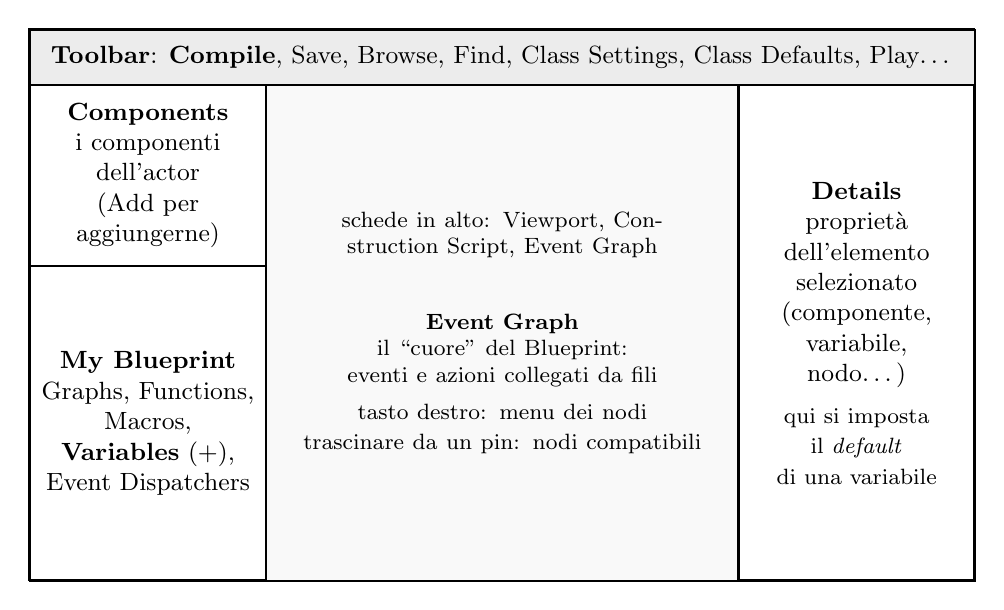
\begin{tikzpicture}[
  font=\small,
  ue2pan/.style={draw, thick, align=center, inner sep=3pt}
]
  \draw[thick] (0,0) rectangle (12,7);
  \node[ue2pan, minimum width=12cm, minimum height=0.7cm, anchor=north west,
    fill=gray!15] at (0,7) {\textbf{Toolbar}: \textbf{Compile}, Save, Browse, Find,
    Class Settings, Class Defaults, Play\ldots};
  \node[ue2pan, minimum width=3cm, minimum height=2.3cm, anchor=north west]
    at (0,6.3) {\textbf{Components}\\i componenti\\dell'actor\\(Add per\\aggiungerne)};
  \node[ue2pan, minimum width=3cm, minimum height=4cm, anchor=north west]
    at (0,4.0) {\textbf{My Blueprint}\\Graphs, Functions,\\Macros,\\
    \textbf{Variables} (+),\\Event Dispatchers};
  \node[ue2pan, minimum width=6cm, minimum height=6.3cm, anchor=north west,
    text width=5.6cm, fill=gray!5] at (3,6.3) {\footnotesize schede in alto:
    Viewport, Construction Script, Event Graph\\[18pt]\textbf{Event Graph}\\il ``cuore'' del Blueprint:\\
    eventi e azioni collegati da fili\\[4pt]\footnotesize tasto destro: menu dei nodi\\
    \footnotesize trascinare da un pin: nodi compatibili};
  \node[ue2pan, minimum width=3cm, minimum height=6.3cm, anchor=north west]
    at (9,6.3) {\textbf{Details}\\proprietà\\dell'elemento\\selezionato\\
    (componente,\\variabile,\\nodo\ldots)\\[4pt]\footnotesize qui si imposta\\
    \footnotesize il \emph{default}\\\footnotesize di una variabile};
\end{tikzpicture}
\caption{L'editor dei Blueprint (Blueprint Class Editor), ricostruito dalla lezione e
dal primo capitolo del libro di Romero e Sewell. La disposizione dei pannelli si può
cambiare, come nel Level Editor.}
\label{ue2:fig:editorbp}
\end{figure}

\paragraph{Approfondimento: i pannelli dell'editor.} Romero e Sewell, nel primo capitolo,
elencano i pannelli principali del \emph{Blueprint Class Editor}: la
\textbf{Toolbar}, i \textbf{Components} (i componenti già pronti che si aggiungono con
Add: \emph{mesh} statiche, luci, suoni, collisioni, particelle, camere), \textbf{My
Blueprint} (dove si creano variabili, macro, funzioni e grafi, con i pulsanti +), i
\textbf{Details} (le proprietà dell'elemento selezionato, con una barra di ricerca in
alto), la \textbf{Viewport} e l'\textbf{Event Graph}. Nell'Event Graph, notano gli
autori, un \textbf{evento} è un nodo \textbf{rosso}, e le altre azioni che seguono un
evento si collegano con dei fili; ci si sposta nel grafo trascinando con il tasto
destro. Di ogni evento se ne può mettere \textbf{uno solo} per grafo, ma si possono
creare eventi propri (\textbf{Add Custom Event}). Oltre a BeginPlay e Tick, il libro
cita gli eventi di \textbf{collisione} (quando due actor si scontrano o si
sovrappongono), gli eventi di \textbf{input} (tastiera, mouse, \emph{touch},
\emph{gamepad}) ed \textbf{Event End Play}, quando l'actor sta per essere rimosso.

% ---------------------------------------------------------------------
\section{Il primo nodo: Print String}
\label{ue2:sec:print}

``Andremo a fare una piccola prova.'' Unreal gestisce tutto con i \textbf{nodi}. Se si
porta il mouse sul ``pinnetto'' bianco a forma di freccia dell'Event BeginPlay, lo si
clicca e lo si \textbf{trascina verso l'esterno}, al rilascio compare un menu con tutti
i blocchi che si possono collegare: ``possiamo metterci tutto quello che vogliamo, tutti
i blocchi che ci serviranno per fare un'azione''.

\paragraph{Print String.} L'azione più semplice è \textbf{Print String}, che
``letteralmente ci stampa qualcosa a schermo''. Il testo predefinito è ``Hello''.

\paragraph{La barra ``Development Only''.} Igor fa notare un dettaglio. A differenza di
altri nodi, come \textbf{Set Actor Location} o \textbf{Enable Collision}, il Print String
ha una \textbf{barra in basso}. Vuol dire che quel blocco ha effetto \textbf{solo in
modalità di sviluppo}: quando si sviluppa e si va in Play nell'editor funziona, ma se si
facesse un \textbf{eseguibile} da mandare a qualcun altro ``questa cosa non avverrà
mai''. Gli altri nodi, invece, sì.

\paragraph{Compilare.} ``Molto importante'': quando si fanno dei cambiamenti
importanti bisogna \textbf{compilare} (\textbf{Compile}, in alto a sinistra). La
compilazione ``legge quello che abbiamo fatto'' e aggiorna il programma; in molti casi
Unreal lo fa anche in automatico, ma conviene farlo sempre. E \textbf{salvare},
``ovviamente, sempre buona cosa''.

\paragraph{La prova.} Si abbassa la finestra del Blueprint, si \textbf{mette l'actor
nella scena} (``ovviamente, se no non succede niente'': il Blueprint è solo una classe,
finché non se ne mette una copia nel livello non esiste) e si preme Play. In alto a
sinistra compare ``Hello'', ma per pochissimo. Igor cambia allora il parametro
\textbf{Duration} del nodo a 100 secondi, e la scritta resta: ``è piccolo'', ma c'è.
L'actor è entrato in funzione e ha fatto la sua azione appena ha cominciato a esistere,
cioè subito, perché era già nella scena.

\paragraph{Una finestra di gioco separata.} ``Se vi è più comodo'', si può far partire il
gioco in una finestra esterna: dai \textbf{tre puntini} accanto al pulsante Play si
sceglie \textbf{New Editor Window (PIE)}. ``Io lo trovo molto più comodo'': invece di
abbassare e rialzare la finestra del Blueprint, il gioco gira in una finestra a parte da
cui si controlla tutto. Igor lo scrive anche in chat.

\paragraph{Approfondimento: \emph{development} e \emph{shipping}.} La barra del Print
String rimanda a una distinzione che Romero e Sewell spiegano nel capitolo sul
\emph{packaging}: le \emph{build} di \textbf{sviluppo} (\emph{Development}) contengono
informazioni che servono al \emph{debug}, quelle di \textbf{distribuzione}
(\emph{Shipping}) sono più ``pulite'', senza informazioni di \emph{debug}, e sono quelle
da pubblicare. I nodi marcati \emph{Development Only}, come il Print String, vengono
semplicemente ignorati in una \emph{build} Shipping: si possono quindi lasciare nel
grafo mentre si lavora senza che il giocatore finale veda mai le scritte di prova.

% ---------------------------------------------------------------------
\section{Le variabili: GET e SET, colori e calcoli}
\label{ue2:sec:variabili}

\paragraph{Che cos'è una variabile.} Igor chiede chi abbia mai sentito parlare di
variabili \emph{bool}, \emph{float}, \emph{int}; qualcuno sì. Una \textbf{variabile} è
``uno slot di una tipologia di valore'' in cui si può mettere un valore: ``è come una
\textbf{scatola}''. Si creano delle piccole scatoline in cui mettere dei valori, ma ogni
scatola è fatta per un certo contenuto: ``c'è la scatola per i gioielli, c'è la scatola
per le praline'' (``mi invento un po' di cose''). Il tipo della variabile decide che cosa
ci si può mettere dentro.

\paragraph{Creare una variabile.} L'esempio: rendere ``esterna'' la durata del Print
String, cioè metterla in una variabile. Nel pannello My Blueprint, alla voce
\textbf{Variables}, si clicca \textbf{+}: si crea subito una variabile, di tipo booleano
oppure dello stesso tipo dell'ultima variabile creata. Igor la chiama \textbf{duration
time text}\footnote{Così nella trascrizione (una volta ``duration time next''); il nome
esatto digitato non si sente, ma non ha importanza per l'esempio.}.

\paragraph{GET e SET.} Se si trascina la variabile nel grafo, Unreal chiede se si vuole
un \textbf{GET} o un \textbf{SET}. GET è \textbf{prendere} il valore che c'è dentro; SET
è \textbf{impostare} il valore dentro. Per dare il valore alla durata del Print String
serve un GET.

\paragraph{I colori devono combaciare.} ``Però attenzione, che succede? Questo è rosso e
questo è verde.'' Il pin della variabile appena creata è \textbf{rosso} (è una
booleana), quello della Duration è \textbf{verde}: ``non sono della stessa tipologia''.
Due pin rossi si collegano; un rosso e un verde no. Il verde è il \textbf{float}. ``Cosa
sono i numeri float?'' ``I numeri con la virgola.'' ``Ottimo'': i numeri con i
\textbf{decimali}. Si cambia quindi il tipo della variabile in Float, il pin diventa
verde, e ``guardate un po', si collega''.

\paragraph{\emph{Please compile the Blueprint}.} Appena collegata, la variabile mostra
l'avviso \emph{please compile the blueprint}: è stata appena creata, e il Blueprint ``non
sa ancora che c'è una variabile nuova''. Dopo la compilazione, nei Details compare il
suo \textbf{valore predefinito} (\emph{Default Value}): ``guarda, questo è il tuo valore.
Quanto lo vuoi?'' Igor mette 10. In Play la scritta dura 10 secondi (``un po' tanti'') e
poi scompare: ``non è più 100''. La lezione: si possono creare variabili, impostarle e
darle ai blocchi di esecuzione.

\paragraph{Nodi di esecuzione e nodi di calcolo.} I \textbf{blocchi di esecuzione} si
riconoscono perché hanno l'intestazione \textbf{blu} e il pin di esecuzione, ``la
freccettina'' bianca. Ci sono però anche nodi \textbf{verdi} senza quel pin: sono nodi
che ``\textbf{calcolano solamente}''. Igor ne fa vedere uno, \textbf{Find Look at
Rotation}: chiede due variabili di un tipo e ne restituisce un'altra, dello stesso tipo
o di un altro. ``Oppure, esempio classico'': gli \textbf{operatori} aritmetici, il
\textbf{+}, il \textbf{$-$} (\emph{Subtraction}), il \textbf{per}, che si cerca con
l'\textbf{asterisco} (\emph{Multiply}), e il \textbf{diviso} (\emph{Divide}). Si
possono invocare tutti gli operatori che servono (figura~\ref{ue2:fig:pin}).

\paragraph{Sottrarre due secondi.} L'esempio: ``indipendentemente da quanto tempo noi
mettiamo qua dentro'', togliere sempre 2 secondi. Si prende il nodo meno, si collega la
variabile al primo ingresso (il nodo ``è diventato verde'', perché ha riconosciuto che si
tratta di un float, e ``ci chiede: te lo sottraggo di un altro float''), si scrive 2 nel
secondo e si collega il risultato alla Duration.

\paragraph{Da numero a testo.} Si può anche \textbf{stampare} il valore: collegando il
float all'ingresso di testo del Print String, Unreal inserisce in automatico un
\textbf{convertitore}. I pin \textbf{rosa} sono le \textbf{stringhe}, cioè testo. In
Play, il Print String non stampa più ``Hello'' ma \textbf{8}, ``che è 10 meno 2'', e la
scritta dura 8 secondi. (Ogni volta che Igor apre Unreal, Zoom va a scatti: ``a quanto
pare mi lagga Zoom benissimo''.)

\begin{figure}[htbp]
\centering
\begin{tikzpicture}[
  font=\small,
  ue2node/.style={draw, thick, rounded corners=4pt, align=center},
  ue2exec/.style={-{Stealth[length=2.5mm]}, very thick},
  ue2flt/.style={-{Stealth[length=2mm]}, thick, green!50!black},
  ue2str/.style={-{Stealth[length=2mm]}, thick, magenta}
]
  \node[ue2node, fill=red!15, minimum width=2.6cm, minimum height=1.2cm]
    (bp) at (0,0) {\textbf{Event}\\\textbf{BeginPlay}};
  \node[ue2node, fill=blue!10, minimum width=3.4cm, minimum height=2.6cm,
    anchor=north west] (pr) at (7.4,0.6) {};
  \node[font=\small\bfseries, anchor=north] at (pr.north) {Print String};
  \node[font=\footnotesize, anchor=west] (ins) at (7.5,-0.5) {In String};
  \node[font=\footnotesize, anchor=west] (dur) at (7.5,-1.2) {Duration};
  \node[font=\scriptsize\itshape, anchor=south] at (pr.south) {Development Only};
  \node[ue2node, fill=green!10, minimum height=0.8cm] (get) at (0.4,-1.9)
    {GET duration (float)};
  \node[ue2node, fill=green!10, minimum height=0.8cm] (minus) at (3.6,-1.9)
    {$x - 2$};
  \node[ue2node, fill=magenta!8, minimum height=0.8cm, font=\footnotesize]
    (conv) at (5.6,-0.5) {float $\to$ string};
  \draw[ue2exec] (bp.east) -- node[above, font=\footnotesize]{esecuzione}
    (bp.east -| pr.west);
  \draw[ue2flt] (get) -- (minus);
  \draw[ue2flt] (minus.east) -- ++(0.4,0) |- (dur.west);
  \draw[ue2flt] (minus.north) |- (conv.west);
  \draw[ue2str] (conv.east) -- (ins.west);
\end{tikzpicture}
\caption{Il primo grafo della lezione, nella sua versione finale: all'inizio del gioco
l'actor stampa la durata meno 2 (cioè 8) per 8 secondi. La freccia nera è il filo di
\textbf{esecuzione} (l'ordine delle azioni, da sinistra a destra); le frecce colorate
sono fili di \textbf{dati}, del colore del loro tipo (verde il float, rosa la stringa).
Il nodo blu, con il pin di esecuzione, è un'\textbf{azione}; i nodi verdi, senza, sono
nodi di \textbf{calcolo}, che si eseguono quando un'azione chiede il loro valore. Il
convertitore è inserito da Unreal in automatico. Schema ricostruito, non copia della
schermata.}
\label{ue2:fig:pin}
\end{figure}

% ---------------------------------------------------------------------
\section{Primo esercizio: Time To Print}
\label{ue2:sec:esercizio1}

``Vorrei fare un piccolo esercizio con voi. Molto velocissimo.''

\paragraph{Staccare un filo.} Prima, un comando: per \textbf{staccare} un collegamento
si tiene premuto \textbf{Alt} e si clicca sul pin.

\paragraph{La consegna.} Creare un'altra variabile, \textbf{time to print}, di tipo
\textbf{float}; staccare la variabile della durata dall'ingresso del testo e collegarci
invece time to print; dare a time to print il valore \textbf{5}, che dovrà essere
stampato a schermo. Anche la Duration va messa a 5. ``Senza che andiamo a vedere poi
ognuno'': l'importante è che ognuno dica ``stampa 5, sì''.

\paragraph{Un esercizio guidato.} Uno studente arriva in ritardo (``scusate, non
riuscivo ad entrare''). A una studentessa il Print String stampa \textbf{0}, e Igor la
guida passo per passo in condivisione dello schermo: fermare il gioco (lo
\textbf{Stop}, o il tasto \textbf{Esc}); creare la variabile dal \textbf{+} di Variables
nel pannello a sinistra; chiamarla time to print; cambiarle il tipo per farla
\textbf{verde}, cioè float (``bravissima''); prenderne il GET; staccare il vecchio
collegamento con Alt e attaccare time to print; compilare (``in alto a sinistra'');
poi, con la variabile selezionata, guardare nei \textbf{Details} a destra: ``vedi, adesso
è apparsa. In fondo''. In fondo ai Details c'è il \textbf{valore predefinito}, ed è lì
che si mette il 5. Lo 0 dipendeva proprio da questo: il valore predefinito di un float
appena creato è zero.

% ---------------------------------------------------------------------
\section{I dettagli di una variabile, e il \emph{tuning}}
\label{ue2:sec:dettagli}

Tutte le caratteristiche di una variabile si vedono nei \textbf{Details}, sia cliccando
la variabile nel grafo, sia cliccandola nella lista Variables. Igor consiglia di
impostare l'engine \textbf{in inglese} (``io sono più abituato all'inglese''), ma se si
trova più facile l'italiano non c'è nessun problema.

\paragraph{Il nome, il tipo, la descrizione.} Nei Details si possono cambiare il nome, il
tipo e una \textbf{descrizione}. La descrizione non la vedrà il giocatore, ma ``i nostri
amici programmatori, o comunque colleghi'': ci si può scrivere un piccolo commento,
come ``variabile da stampare nel Print''. È un'informazione ``per lo più organizzativa'',
``non un qualcosa che troverete spesso''.

\paragraph{Pubblica e privata: Instance Editable.} L'opzione \textbf{Instance Editable}
rende una variabile \textbf{pubblica}. Gli studenti non conoscono la distinzione ``in
questo contesto''. Una variabile \textbf{privata} esiste solo all'interno dell'actor;
una \textbf{pubblica} si può vedere e modificare direttamente nei \textbf{Details}
dell'actor piazzato nel livello. Uno studente chiede se sia come ``globale e locale''.
``Non esattamente, perché globale è anche un'altra cosa che andremo a vedere'': le
variabili davvero globali si fanno con la \textbf{Game Instance}, un oggetto che
\textbf{esiste finché esiste il gioco} e che può contenere variabili da ``dare in pasto''
a tutti gli actor che si vuole.

\paragraph{L'occhietto.} Lo stesso risultato si ottiene con l'icona
dell'\textbf{occhio} accanto alla variabile nella lista. Igor lo mostra: con l'occhio
aperto, selezionando l'actor nel livello, nei Details compare la sezione
\textbf{Default} con \emph{time to print}; con l'occhio chiuso, dopo aver ricompilato,
la voce scompare.

\paragraph{Il \emph{tuning}.} A che cosa serve? ``Il design è sempre con me.'' Come
designer, a Igor è capitato spesso di fare \textbf{\emph{tuning}}: la pratica di
\textbf{aggiustare i valori}, ``quanto danno fa, quanto fa di contrattacco'', in
generale i valori modificabili. Diceva al programmatore: ``lasciami quei valori, che li
devo controllare'', cioè testare. E poi andava nei Details dell'actor e cambiava
``questo, quell'altro, questo, quell'altro''. Le variabili pubbliche servono proprio a
questo: permettono di \textbf{interagire con l'editor stesso} senza toccare il grafo. Le
cose private, invece, restano nel campo dell'actor.

\paragraph{Approfondimento: gli attributi di una variabile.} Romero e Sewell, nel secondo
capitolo, elencano tutti gli attributi che i Details mostrano per una variabile.
\begin{itemize}
  \item \textbf{Variable Name} e \textbf{Variable Type}: il nome e il tipo. I Blueprint
        sono un linguaggio \textbf{fortemente tipizzato}: il tipo si sceglie alla
        creazione e non cambia durante l'esecuzione.
  \item \textbf{Instance Editable}: se attivo, \textbf{ogni copia} del Blueprint
        piazzata nel livello può avere un valore diverso; altrimenti tutte le copie
        (le \emph{istanze}) condividono lo stesso valore iniziale. È la precisazione
        tecnica del ``pubblico'' di Igor.
  \item \textbf{Blueprint Read Only}: se attivo, i nodi non possono modificare la
        variabile.
  \item \textbf{Tooltip}: il testo che compare passando il mouse sulla variabile; è la
        ``descrizione'' di cui parla Igor.
  \item \textbf{Expose on Spawn}: la variabile si può impostare nel momento in cui
        l'actor viene \emph{spawnato}.
  \item \textbf{Private}: se attivo, i Blueprint figli non possono modificarla.
  \item \textbf{Expose to Cinematics}: la rende visibile al Sequencer.
  \item \textbf{Category}: per raggruppare le variabili.
  \item \textbf{Slider Range} e \textbf{Value Range}: il minimo e il massimo, per lo
        \emph{slider} e per i valori ammessi. Per il \emph{tuning} sono preziosi: chi
        aggiusta i valori non può uscire dai limiti sensati.
  \item \textbf{Replication}: per i giochi in rete.
  \item \textbf{Default Value}: il valore iniziale; si può impostare solo dopo aver
        compilato, come si è visto nell'esercizio.
\end{itemize}

% ---------------------------------------------------------------------
\section{I tipi di variabile}
\label{ue2:sec:tipi}

Igor cancella tutto (seleziona e preme \textbf{Canc}, \emph{Delete} sulla tastiera
inglese) e passa a una slide sui tipi di variabile (tabella~\ref{ue2:tab:tipi}).
``Immaginiamoci sempre delle scatolette, con dentro dei valori.''

\paragraph{Booleana.} ``Qualcuno ha mai sentito parlare di booleane?'' Qualche sì,
qualche no. Una variabile \textbf{booleana} ha due valori possibili: \textbf{vero} o
\textbf{falso}. ``Dentro o c'è vero, o c'è falso, una delle due. Basta.'' Con un esempio
dall'elettrotecnica, è ``letteralmente lo \emph{switch} della luce'': spento è falso,
acceso è vero; a livello di circuito, ``è aperto o è chiuso''.

\paragraph{Byte, Integer, Integer64.} Il \textbf{byte} è un valore numerico intero
compreso tra 0 e 255. L'\textbf{integer}\footnote{Nella trascrizione ``gli integrali, i
numeri integrali''.}, o intero, è un numero \textbf{senza la virgola}: ``1, 2, 3, 4, 5,
6, 7, 8, senza virgola, senza niente'', compreso tra $-2^{31}$ e $2^{31}$ (``possiamo
anche non capire qual è il numero preciso, perché tanto è difficile che ci arriviamo'').
L'\textbf{integer64} arriva a 64 bit, tra $-2^{63}$ e $2^{63}$.

\paragraph{Float.} Il \textbf{float} è il valore numerico \textbf{con i decimali}.

\paragraph{Name, String, Text.} Il \textbf{name} è un testo usato principalmente per gli
\textbf{identificatori}, per identificare degli elementi in Unreal. La \textbf{string}
è un gruppo di caratteri \textbf{alfanumerici}, ``numeri e lettere''. Uno studente chiede
la differenza: anche il name è una stringa? La stringa, risponde Igor, si usa per lo più
nei \textbf{testi}; i name sono \textbf{nomenclature}: ``il nome di un livello, il nome
di un \emph{asset}''. ``Tipo un'etichetta'', propone lo studente: ``bravissimo, è come
un'etichetta'', ``quasi come un \textbf{tag}''. Il \textbf{text}, infine, è un testo
usato principalmente nella \textbf{UI}, la \emph{user interface}: tutto ciò che è 2D e
con cui l'utente interagisce, un termine usato ``in tanti campi, anche coi siti''.

\paragraph{Vector, Rotator, Transform.} I \textbf{vettori} sono ``molto importanti'',
essendo Unreal un ambiente tridimensionale. Un vettore può essere la
\textbf{locazione}: ``ci ricordiamo che quando abbiamo spostato i nostri cubetti e coni
abbiamo visto quei tre valori cambiare, la X, la Y e la Z?'' Un vettore è ``la
composizione'' di questi tre: una variabile che contiene \textbf{tre valori}, X, Y e Z.
Il \textbf{rotator} contiene gli X, Y e Z della \textbf{rotazione} (``poi faremo un po'
di discorsi, perché esistono i quaternioni, eccetera''). Il \textbf{transform}
contiene location, rotation e scala.

\paragraph{Object.} Infine il tipo \textbf{object}: ``volendo, noi potremmo creare una
variabile di tipologia di un actor che abbiamo creato''. È una variabile che contiene un
\textbf{riferimento} a un actor (si vedrà con il Level Blueprint,
sezione~\ref{ue2:sec:level}).

\begin{table}[htbp]
\centering
\small
\begin{tabular}{@{}p{2.2cm}p{2.0cm}p{8.8cm}@{}}
\toprule
\textbf{Tipo} & \textbf{Colore} & \textbf{Che cosa contiene} \\
\midrule
Boolean & rosso & vero o falso (\emph{true}/\emph{false}) \\
Byte & verde scuro & intero da 0 a 255 (8 bit) \\
Integer & verde acqua & intero da $-2^{31}$ a $2^{31}-1$ (32 bit) \\
Integer64 & verde acqua scuro & intero da $-2^{63}$ a $2^{63}-1$ (64 bit) \\
Float & verde & numero con decimali; in Unreal Engine 5 i Blueprint lo trattano in
  precisione singola o doppia (\emph{Double}) \\
Name & lilla & identificatore, ``etichetta'' (nome di un livello, di un \emph{asset}) \\
String & rosa & gruppo di caratteri alfanumerici \\
Text & rosa scuro & testo per la UI, \textbf{localizzabile} (traducibile) \\
Vector & giallo & tre float X, Y, Z (per esempio una locazione) \\
Rotator & viola-lilla & tre float della rotazione: X (\emph{roll}), Y (\emph{pitch}),
  Z (\emph{yaw}) \\
Transform & arancione & locazione, rotazione e scala \\
Object & blu & riferimento a un oggetto (per esempio un actor nel livello) \\
\bottomrule
\end{tabular}
\caption{I tipi di variabile della slide di Igor, con i colori dei loro pin
nell'editor (i nomi dei colori sono approssimativi) e le integrazioni del libro di
Romero e Sewell (i limiti esatti degli interi, \emph{roll}, \emph{pitch} e \emph{yaw},
la localizzazione del Text).}
\label{ue2:tab:tipi}
\end{table}

\paragraph{Approfondimento: Double, Text e i tre angoli.} Tre precisazioni dal secondo
capitolo del libro. Primo: oltre al Float a 32 bit (sette cifre decimali di
precisione) esiste il \textbf{Double} a 64 bit (sedici cifre); in Unreal Engine 5 l'editor
mostra entrambi come ``Float'' e sceglie la precisione da solo. Secondo: il
\textbf{Text} serve ai testi che saranno \textbf{localizzati}, cioè tradotti in altre
lingue: è per questo che è il tipo della UI, mentre String è il testo ``di servizio'' e
Name l'identificatore. Terzo: i tre valori del \textbf{Rotator} hanno un nome. X è il
\textbf{\emph{roll}} (il rollio, la rotazione attorno all'asse X, quello ``in avanti''),
Y il \textbf{\emph{pitch}} (il beccheggio, attorno all'asse Y, alzare o abbassare il
muso), Z lo \textbf{\emph{yaw}} (l'imbardata, attorno all'asse Z verticale, girare a
destra e a sinistra). Sono i nomi che compariranno nei nodi della piattaforma
(sezione~\ref{ue2:sec:mouse}). I \textbf{quaternioni} a cui accenna Igor sono un altro
modo, matematicamente più robusto, di rappresentare una rotazione: evitano il problema
del \emph{gimbal lock}, in cui due dei tre assi finiscono per coincidere e si perde un
grado di libertà. Unreal li usa al suo interno, ma nei Blueprint si lavora quasi sempre
con i Rotator.

% ---------------------------------------------------------------------
\section{Le booleane e il Branch}
\label{ue2:sec:branch}

``Adesso vi faccio vedere.'' Igor crea una variabile, la chiama ``letteralmente''
\textbf{bool}, e le dà il tipo booleano.

\paragraph{GET e SET in un gesto.} ``Piccola cosetta'': invece di scegliere dal menu, si
può fare un GET ``velocissimamente'' trascinando la variabile nel grafo con
\textbf{Ctrl} premuto, e un SET trascinandola con \textbf{Alt}. Il \textbf{GET} è il pin
che dice ``questa è la scatoletta che c'è dentro qualcosa, prendi il valore da qui''. Il
\textbf{SET} è diverso: ha un \textbf{nodo di esecuzione}, a differenza del GET, e ha una
\textbf{casella di spunta}\footnote{Nella trascrizione ``un TIL'': è il \emph{tick},
la spunta della casella.}: cliccandola si imposta il valore. ``Col SET sto letteralmente
impostando il suo valore'': spunta, vero; niente spunta, falso.

\paragraph{Stampare una booleana.} Igor rifà un Print String con Duration 10 (``sennò è
troppo poco''), collega il pin della booleana al testo e va in Play: in alto a sinistra
compare \textbf{false}. Mette la spunta, rifà Play: \textbf{true}. Il Print String
riceve, tramite la stringa, il valore della variabile.

\paragraph{A che cosa serve sapere se è vero o falso?} ``La domanda magari è: ok, ma che ci
serve?'' Serve perché si possono usare delle \textbf{condizioni}. ``Qualcuno ha mai
sentito parlare di \emph{if}, \emph{else}?'' Edoardo sì: ``ho studiato informatica alle
superiori''. ``Grande, perfetto.'' L'\textbf{if-else} è una condizione, e in Unreal non si
chiama così: tenendo premuto \textbf{B} e cliccando nel grafo compare il
\textbf{Branch}, ``cioè due percorsi''. È ``un \textbf{bivio}'': ``se questa condizione
che abbiamo qua è vera, vai per questo percorso; se questa condizione è falsa, vammi per
un altro''.

\paragraph{Il primo Branch.} Igor collega il Branch dopo il BeginPlay e porta la
variabile bool nel pin rosso \textbf{Condition}. Sull'uscita \textbf{True} mette un Print
String con ``la variabile è vera''; per l'uscita \textbf{False} copia il nodo (``per
copiare qualcosa, Ctrl+C, Ctrl+V, classico'') e scrive ``la variabile è falsa''. Con la
variabile falsa, in Play esce ``la variabile è falsa''; con la spunta, ``la variabile è
vera'' (figura~\ref{ue2:fig:branch}).

\paragraph{I binari del treno.} ``Letteralmente sta prendendo un bivio: o vado di qua, o
vado di là.'' Igor lo paragona ai \textbf{binari di un treno}: ``se la leva è a destra,
vado a destra; se la leva è a sinistra, vado a sinistra. E la nostra leva è la nostra
variabile''. Il bool è molto importante perché permette di avere delle condizioni, e
quindi gli attori ``\textbf{pensano}'': hanno la ``capacità di scelte'', ``ah, ok, allora
prendo questa strada perché ho questa variabile di questo tipo''.

\begin{figure}[htbp]
\centering
\begin{tikzpicture}[
  font=\small,
  ue2node/.style={draw, thick, rounded corners=4pt, align=center,
                  minimum height=1cm},
  ue2exec/.style={-{Stealth[length=2.5mm]}, very thick},
  ue2bool/.style={-{Stealth[length=2mm]}, thick, red!70!black}
]
  \node[ue2node, fill=red!15, minimum width=2.4cm] (bp) at (0,0)
    {\textbf{Event}\\\textbf{BeginPlay}};
  \node[ue2node, fill=gray!10, minimum width=2.2cm, minimum height=1.6cm]
    (br) at (4,0) {\textbf{Branch}\\[2pt]\footnotesize Condition};
  \node[ue2node, fill=green!8, minimum width=1.6cm] (get) at (1.6,-1.8) {GET bool};
  \node[ue2node, fill=blue!10, text width=3.6cm] (pt) at (9,0.9)
    {\textbf{Print String}\\\footnotesize ``la variabile è vera''};
  \node[ue2node, fill=blue!10, text width=3.6cm] (pf) at (9,-0.9)
    {\textbf{Print String}\\\footnotesize ``la variabile è falsa''};
  \draw[ue2exec] (bp) -- (br);
  \draw[ue2bool] (get.east) -| ([xshift=-4mm]br.south);
  \draw[ue2exec] ([yshift=4mm]br.east) -- node[above, font=\footnotesize]{True}
    ++(1.2,0) |- (pt.west);
  \draw[ue2exec] ([yshift=-4mm]br.east) -- node[below, font=\footnotesize]{False}
    ++(1.2,0) |- (pf.west);
\end{tikzpicture}
\caption{Il Branch è un bivio: segue l'uscita True o l'uscita False a seconda del valore
della condizione. ``La nostra leva è la nostra variabile.''}
\label{ue2:fig:branch}
\end{figure}

\paragraph{Si può accedere al codice?} Uno studente chiede se sia possibile accedere anche
al codice, ``immagino che sia C''. Sì, è possibile, ``però non lo faremo''. Con il C++ si
possono definire anche i blocchi stessi, creare blocchi di tipo diverso; ma ``di base, su
Blueprint possiamo farlo allo stesso modo anche noi''. Chi vuole può andare a vederlo; e
c'è chi va ``proprio nel profondo della programmazione'', come gli \emph{engine
programmer}.

\paragraph{Allineare i nodi.} ``Una piccola cosa, se vi piace l'ordine'': si selezionano
due nodi e si preme \textbf{Q}, e Unreal li allinea.

\paragraph{Approfondimento: Branch e operatori relazionali.} Romero e Sewell presentano il
Branch nel secondo capitolo, parlando del \textbf{percorso di esecuzione}: i pin bianchi
sono i \textbf{pin di esecuzione}, gli altri, colorati, i \textbf{pin di dati};
l'esecuzione parte da un evento rosso e segue il filo bianco da sinistra a destra fino
all'ultimo nodo. Alcuni nodi, come il Branch, \textbf{controllano il flusso}: decidono
quale strada prendere. Il loro esempio è un personaggio con una booleana \emph{Has
Shield}: se è vera, il Branch imposta \emph{Shield Value} a 100; se è falsa, a 0. Nella
lezione la condizione è sempre una variabile booleana; nella pratica, spesso, è il
risultato di un \textbf{operatore relazionale}: i nodi $<$, $\leq$, $>$, $\geq$, $=$,
$\neq$ confrontano due valori e restituiscono una booleana. L'esempio del libro: quando
un oggetto subisce danni, un Branch controlla se \emph{Health} $\leq 0$, e in quel caso
l'oggetto viene distrutto; se no, non succede niente, perché all'uscita False non è
collegato nulla. Quanto alla scorciatoia: nel menu che si apre con il tasto destro su
una selezione di nodi c'è la voce \textbf{Alignment}, con allineamenti in alto, al
centro, in basso, a sinistra, a destra, e \textbf{Straighten Connection(s)}, che
raddrizza i fili; il tasto \textbf{Q} è la scorciatoia di quest'ultima. Il libro ricorda
anche le altre scorciatoie ``tasto + clic'': \textbf{B} per il Branch, \textbf{S} per il
nodo Sequence, \textbf{D} per il Delay, \textbf{F} per il For Each Loop
(tabella~\ref{ue2:tab:scorciatoie}).

% ---------------------------------------------------------------------
\section{Gli operatori logici: AND, OR, NOT}
\label{ue2:sec:logici}

Igor cancella i nodi di prova (``tanto non ci sono problemi'') e passa agli
\textbf{operatori logici}. ``Qualcuno ha mai sentito parlare di AND, OR, NOT?'' Sì.

\paragraph{Il gioco dei tubi.} A che cosa servono? Una variabile booleana ha i suoi valori,
vero e falso; ``però mettiamo conto che ne abbiamo altre'', e bisogna metterle in
\textbf{comparazione}. L'esempio è ``il gioco dei tubi'', l'enigma in cui bisogna girare i
tubi nel verso giusto per collegarli. Se ci sono due tubi, per risolvere l'enigma un tubo
deve essere girato nel modo giusto \textbf{e} anche l'altro: sono \textbf{due
condizioni} da prendere insieme. ``Come facciamo a metterle insieme?''

\paragraph{I nodi.} Igor crea una seconda booleana, \textbf{bool 2}. Gli operatori si
cercano scrivendo \textbf{OR Boolean}, \textbf{AND Boolean} e \textbf{NOT Boolean}.
``Questi sono i tre più usati''; ce ne sono altri, come il NOR, ``ma sono un attimo da
vedere poi più avanti''.

\paragraph{OR.} L'OR dice: ``se almeno un valore è vero, allora la condizione finale è
vera''. Con bool vera e bool 2 falsa, collegato alla condizione del Branch, esce ``la
variabile è vera''. È ``un modo per sommare le variabili tra \emph{true} e \emph{false}'',
``una specie di somma, chiamiamola così'': ``letteralmente dice: o questa, o questa''.

\paragraph{AND.} L'AND, con gli stessi valori, vero e falso, dà ``la variabile è falsa'',
``perché AND vuol dire \emph{questa e questa}'': tutte le condizioni devono essere vere
perché il risultato sia vero. Igor mette vera anche la seconda e\ldots{} non succede
niente: ``scusate, questo non l'ho collegato, sono io''. Collegato, esce ``la variabile è
vera''. Ricapitolando: se tutte e due sono vere, è vero; se una sola è falsa, ``tutto
quanto è falso''; se tutte e due sono false, è falso (``doppio falso'').

\paragraph{NOT.} Il NOT ha un solo ingresso e ``letteralmente \textbf{inverte}'': se la
variabile è vera diventa falsa, se è falsa diventa vera. Collegato a una variabile vera,
dà falso. ``Non lo useremo tanto.'' La tabella~\ref{ue2:tab:logici} riassume i tre
operatori.

\begin{table}[htbp]
\centering
\small
\begin{tabular}{@{}cc|ccc|ccc@{}}
\toprule
\textbf{A} & \textbf{B} & \textbf{A OR B} & \textbf{A AND B} & \textbf{NOT A} &
  \textbf{A NOR B} & \textbf{A NAND B} & \textbf{A XOR B} \\
\midrule
falso & falso & falso & falso & vero  & vero  & vero  & falso \\
falso & vero  & vero  & falso & vero  & falso & vero  & vero  \\
vero  & falso & vero  & falso & falso & falso & vero  & vero  \\
vero  & vero  & vero  & vero  & falso & falso & falso & falso \\
\bottomrule
\end{tabular}
\caption{Le tabelle di verità degli operatori logici. Le prime tre colonne di risultati
sono gli operatori della lezione; le ultime tre sono un'integrazione dal libro di Romero
e Sewell.}
\label{ue2:tab:logici}
\end{table}

\paragraph{Approfondimento: NOR, NAND, XOR, e perché l'OR è una ``somma''.} Il libro
completa la lista degli operatori logici dei Blueprint con tre combinazioni. Il
\textbf{NOR} (NOT + OR) è vero solo se entrambi gli ingressi sono falsi; il \textbf{NAND}
(NOT + AND) è falso solo se entrambi sono veri; lo \textbf{XOR}, l'OR esclusivo, è vero
se i due ingressi sono \textbf{diversi}. L'esempio del libro per l'AND: un Print String
che si esegue solo se \emph{Health} $> 70$ \textbf{e} \emph{Shield Value} $> 50$, con
due operatori relazionali che alimentano un AND. Quanto alla ``somma'' di Igor, è
un'intuizione che ha un nome: nell'\textbf{algebra di Boole}, da cui il tipo
\emph{boolean} prende il nome, l'OR si scrive come una somma ($A + B$) e l'AND come un
prodotto ($A \cdot B$). Se si leggono vero e falso come 1 e 0, l'AND si comporta
esattamente come una moltiplicazione (basta uno 0 per fare 0), e l'OR come una somma
in cui ``1 + 1'' resta 1.

% ---------------------------------------------------------------------
\section{Secondo esercizio: due Branch, OR e AND}
\label{ue2:sec:esercizio2}

``Allora facciamo un piccolo esercizio.''

\paragraph{La consegna.} All'Event BeginPlay si collega un \textbf{SET} della variabile
bool (quello che si ottiene trascinandola con Alt), e il suo valore va alla condizione
di un \textbf{primo Branch}. Su ciascuna uscita del primo Branch va un \textbf{secondo
Branch}: su True un Branch la cui condizione è \textbf{bool OR bool 2}; su False un
Branch la cui condizione è \textbf{bool AND bool 2}. Solo se il secondo Branch è vero si
stampa, e invece di ``la variabile è vera'' si stampa \textbf{il valore finale} del
calcolo, collegando l'uscita dell'operatore all'In String
(figura~\ref{ue2:fig:esercizio2}). ``Ce la fate?'' Cinque minuti.

\begin{figure}[htbp]
\centering
\begin{tikzpicture}[
  font=\small,
  ue2node/.style={draw, thick, rounded corners=4pt, align=center,
                  minimum height=0.9cm},
  ue2exec/.style={-{Stealth[length=2.5mm]}, very thick},
  ue2bool/.style={-{Stealth[length=2mm]}, thick, red!70!black}
]
  \node[ue2node, fill=red!15] (bp) at (0,0) {\textbf{BeginPlay}};
  \node[ue2node, fill=blue!10] (set) at (2.6,0) {\textbf{SET bool}\\\footnotesize
    $\square$ / $\checkmark$};
  \node[ue2node, fill=gray!10] (b1) at (5.2,0) {\textbf{Branch 1}\\\footnotesize
    cond.\ = bool};
  \node[ue2node, fill=gray!10] (b2) at (8.4,1.5) {\textbf{Branch 2}};
  \node[ue2node, fill=gray!10] (b3) at (8.4,-1.5) {\textbf{Branch 3}};
  \node[ue2node, fill=green!8] (or) at (8.4,3.1) {bool \textbf{OR} bool 2};
  \node[ue2node, fill=green!8] (and) at (8.4,-3.1) {bool \textbf{AND} bool 2};
  \node[ue2node, fill=blue!10, text width=2.3cm] (p1) at (11.6,1.5)
    {\textbf{Print}\\\footnotesize risultato OR};
  \node[ue2node, fill=blue!10, text width=2.3cm] (p2) at (11.6,-1.5)
    {\textbf{Print}\\\footnotesize risultato AND};
  \draw[ue2exec] (bp) -- (set);
  \draw[ue2exec] (set) -- (b1);
  \draw[ue2exec] (b1.east) ++(0,0.2) -- ++(0.5,0) |- node[pos=0.75, above,
    font=\footnotesize]{True} (b2.west);
  \draw[ue2exec] (b1.east) ++(0,-0.2) -- ++(0.5,0) |- node[pos=0.75, below,
    font=\footnotesize]{False} (b3.west);
  \draw[ue2bool] (or) -- (b2);
  \draw[ue2bool] (and) -- (b3);
  \draw[ue2exec] (b2) -- node[above, font=\footnotesize]{True} (p1);
  \draw[ue2exec] (b3) -- node[below, font=\footnotesize]{True} (p2);
  \draw[ue2bool, dashed] (or.east) -| (p1.north);
  \draw[ue2bool, dashed] (and.east) -| (p2.south);
\end{tikzpicture}
\caption{Il secondo esercizio. Le frecce nere sono l'esecuzione, quelle rosse i valori
booleani (tratteggiate: il risultato dell'operatore, convertito in testo e stampato). Le
uscite False dei Branch 2 e 3 non sono collegate: in quei casi non si stampa niente.}
\label{ue2:fig:esercizio2}
\end{figure}

\paragraph{Le domande durante l'esercizio.} Lo studente arrivato in ritardo chiede come
si crea il Print String: tasto destro, Print String. Un altro si è perso gli operatori:
si scrivono proprio ``AND Boolean'', ``OR Boolean'', ``NOT Boolean''. Una studentessa non
ricorda come si prende ``l'oggetto con il pallino rosso'' (la variabile): ``mettilo qua
dentro, ti appare in automatico''. Trascinando la variabile direttamente sul pin, Unreal
crea da solo il GET.

\paragraph{La spunta che non c'entra.} Un'altra studentessa ha un problema: sul primo
Branch, nella condizione, ha una \textbf{spunta} che Igor non ha. Il pin Condition non è
collegato all'\textbf{uscita} del SET. ``Devi collegare questo pallino a questo
pallino.'' Igor spiega che cosa è successo, con una dimostrazione. Il nodo SET ha a
destra un pin di uscita: ``è il valore che io gli ho impostato'', che esce dal nodo
``come un collegamento''. Il Branch ha a sinistra ``un posto in cui posso mettere quel
valore''. Se il pin non è collegato, la casella di spunta del Branch è una
\textbf{condizione interna al Branch}, che non ha niente a che vedere con la variabile:
``la porta si aprirà secondo bool, non secondo questa condizione qua''. Igor mette la
variabile a vero e la spunta del Branch a falso: il Print String collegato al True
``non mi stampa niente'', ``perché questa qua non è relativa a questa''. Collegando il
pin, stampa. (``Stavo impazzendo perché non mi stampava niente.'')

\paragraph{I ``what if''.} Poi Igor cerca ``un candidato'' per una piccola verifica:
``se io adesso vi cambio un po' i parametri, dove andiamo a finire con tutte le linee?''
Si offre uno studente.
\begin{itemize}
  \item \textbf{bool vero, bool 2 falso.} ``Siccome è \emph{true}, finisce sopra, sul
        primo Branch'' (il Branch 2 della figura). ``Controlla se tra bool e bool 2 uno
        dei due è vero. In questo caso lo è, perché hai settato bool come vero. Il
        secondo non è importante.'' Quindi va su True e stampa il valore. ``Perfetto.
        Netto, liscio.''
  \item \textbf{bool falso.} ``False scende giù e controlla se entrambi, bool e bool 2,
        sono veri. In questo caso bool è falso, quindi anche qui il secondo valore non
        è importante, perché uno dei due è falso. Il risultato dell'AND è falso e non
        stampa niente.'' ``Esatto, perfetto.''
\end{itemize}
La morale: ``indipendentemente dalle condizioni, possiamo cambiare i binari di un
percorso di programmazione''. È ``una delle cose più principali'', e serve molto spesso
per \textbf{diversificare i comportamenti} dei Blueprint. Igor chiede ancora se ci sono
domande, e decide di non cancellare il grafo ma di lasciarlo lì, scollegato. ``Sono stato
chiaro, dai.''

\paragraph{Approfondimento: la valutazione ``pigra''.} Lo studente coglie, senza
nominarlo, un principio importante: in un OR, se il primo ingresso è vero il secondo
``non è importante''; in un AND, se il primo è falso il secondo non cambia il risultato.
In molti linguaggi di programmazione questo si chiama \emph{short-circuit evaluation}
(valutazione a corto circuito): il secondo operando non viene nemmeno calcolato. Nei
nodi Blueprint, attenzione, i due ingressi vengono comunque calcolati entrambi; ma il
ragionamento sul \emph{risultato} è lo stesso, ed è quello che serve per prevedere dove
andrà l'esecuzione.

% ---------------------------------------------------------------------
\section{Il Level Blueprint e la piattaforma}
\label{ue2:sec:level}

``Adesso andremo a fare una piccola cosa direttamente nel nostro bellissimo Blueprint.''
L'obiettivo è una \textbf{piattaforma} che \textbf{ruota}, cioè si inclina, ``a seconda
di quanto premiamo'' dei tasti (D, A, e così via).

\paragraph{La piattaforma.} Si prende un \textbf{cubo} dal pannello Place Actors, lo si
mette in scena e lo si allarga ``quanto volete'', fino a farne una piattaforma.

\paragraph{Il Level Blueprint.} ``Vi farò conoscere il bellissimo mondo del \textbf{Level
Blueprint}.'' In Unreal esiste anche un Blueprint \textbf{interno al livello}: quando si
apre quel livello, al suo interno ci sono delle regole (``spawna qualcosa'', eccetera).
Lo si apre dall'icona dei Blueprint nella barra in alto: \textbf{Open Level Blueprint}.
Una studentessa si è persa (``scusa, come lo apriamo?''), e Igor le mostra l'icona.

\paragraph{Un evento di input.} Si è parlato di eventi con le loro condizioni; uno dei più
semplici è l'\textbf{input}. Tasto destro nel grafo, si scrive \textbf{W} e si sceglie
la voce con ``l'immaginetta della tastierina'' e la W: è un evento che scatta
\textbf{alla pressione del tasto W}.

\paragraph{La referenza.} Ma come si dice al grafo che deve agire su \emph{quella}
piattaforma? Si crea una \textbf{referenza}. Con il cubo selezionato nel livello, nel
Level Blueprint si fa tasto destro e si sceglie \textbf{Create a Reference to Cube94}
(il cubo di Igor si chiama Cube94, e lo si ritrova con quel nome nell'Outliner). ``Questo
può essere fatto solo nel Level Blueprint, ve lo dico.''

\paragraph{Set Actor Rotation e i suoi pin.} Dalla referenza si trascina un filo e si
sceglie \textbf{Set Actor Rotation}. Il nodo ha tre pin di dati:
\begin{itemize}
  \item un pin \textbf{blu}, il \textbf{Target}: un \emph{Actor Object Reference}, cioè
        una variabile che si riferisce a un actor, a uno qualunque degli elementi della
        \emph{viewport}, ``che abbiano programmazione o meno''. È l'actor su cui il nodo
        agisce;
  \item un pin \textbf{lilla}, \textbf{New Rotation}: un \textbf{rotator}, la
        composizione degli assi X, Y e Z della rotazione;
  \item un pin \textbf{rosso}, un \textbf{bool}: \textbf{Teleport} (tornerà utile con
        la fisica, sezione~\ref{ue2:sec:fisica}).
\end{itemize}

\paragraph{Il Player Start.} Per vedere la piattaforma serve un punto da cui partire.
``Prendete il \textbf{Player Start}'': lo si trova nel Place Actors, o cercandolo, ed è
``un controllone'' (l'icona di un \emph{joystick}). Lo si mette davanti alla piattaforma
e lo si gira verso di essa.

\paragraph{Consume Input.} Selezionando l'evento W, nei Details c'è una casella
interessante, \textbf{Consume Input}. Se è spuntata, il tasto W ``sarà dedicato solo a
questo evento'': il giocatore non potrà più usarlo per muoversi in avanti. Senza la spunta
si muoverebbe ``avanti e indietro''; ``a noi interessa stare fermi'', quindi la spunta
resta.

\paragraph{Quale asse, e in che verso.} La piattaforma va ruotata attorno all'asse
\textbf{X}. In positivo o in negativo? Igor lo verifica nella \emph{viewport} ruotando il
cubo: in un verso la rotazione è negativa, nell'altro positiva. ``Per come mi regolo'',
W manda la piattaforma in avanti, quindi si piega in un verso, e indietro nell'altro.
Igor scrive 5 nella X del New Rotation e prova.

% ---------------------------------------------------------------------
\section{La mobilità: Static, Stationary, Movable}
\label{ue2:sec:mobilita}

Non funziona, ``giustamente'', e Unreal mostra un avviso: ``ricordate che questo che mi è
appena uscito è un problema che Unreal ci darà sempre''. L'actor non ha la capacità di
essere \textbf{Movable}: non si può muovere nel mondo.

\paragraph{Dove si trova.} Nel \emph{transform} dell'actor, sotto location, rotation e
scala, c'è la \textbf{Mobility}, con tre valori: \textbf{Static}, \textbf{Stationary} e
\textbf{Movable}. È ``la tipologia di oggetto'' rispetto a come reagisce al mondo, e
riguarda ``soprattutto il rendering''.
\begin{itemize}
  \item \textbf{Static.} L'oggetto sa che non si muoverà. Quando si calcolano le luci,
        la sua ombra viene calcolata una volta e poi è come \textbf{dipinta}: ``è
        dipinta''. ``Per alleggerirsi la cosa'', l'engine dice: è un oggetto statico,
        ``basta che mi calcolo una volta l'ombra e basta''.
  \item \textbf{Stationary.} Una via di mezzo: le ombre vengono messe in
        \emph{cache}\footnote{Nella trascrizione ``vengono chesciate'': con ogni
        probabilità ``cachate'', dall'inglese \emph{cached}.}, l'oggetto può essere
        cambiato, ma non può essere mosso.
  \item \textbf{Movable.} Totalmente \textbf{dinamico}.
\end{itemize}
La piattaforma va messa su \textbf{Movable}, e allora ruota di 5 gradi. Igor prova con
valori più grandi (``facciamo tipo 25'') per vederlo meglio.

\paragraph{Approfondimento: la mobilità secondo il libro.} Romero e Sewell incontrano lo
stesso problema nel quinto capitolo, quando un bersaglio cilindrico deve cominciare a
muoversi: bisogna prima portare la sua Mobility da Static a \textbf{Movable}, nei Details
sotto il TRANSFORM. E aggiungono una nota importante: gli actor di base piazzati nel
mondo sono \textbf{Static per impostazione predefinita}, e gli oggetti statici sono
``significativamente meno costosi'' da renderizzare; per questo Static dovrebbe essere
la scelta predefinita per tutto ciò che non è interattivo, per tenere alto il
\emph{frame rate}. Stationary ha senso soprattutto per le \textbf{luci}: una luce
Stationary non si sposta, ma se ne possono cambiare colore e intensità durante il gioco,
e parte della sua illuminazione è precalcolata. Movable va riservato agli oggetti che
devono davvero muoversi.

% ---------------------------------------------------------------------
\section{Ruotare di 5 gradi a ogni pressione: Split Struct Pin}
\label{ue2:sec:split}

\paragraph{Funziona una volta sola.} ``Però che succede? Guardate un po'.'' Se si preme
di nuovo W, la piattaforma non fa niente. Il problema è che la si sta impostando a un
\textbf{valore preciso}: Set Actor Rotation dice ``mettiti a 25 gradi'', e la seconda
volta la piattaforma risponde ``ci sto già, a 25''. Serve invece una rotazione che
\textbf{parta da quella attuale}.

\paragraph{Prendere i valori dell'actor.} Igor mostra che dalla referenza di un actor si
possono prendere \textbf{tutti} i suoi valori: la location, la rotation, la scala, la
\emph{mesh}, i materiali (``che poi vedremo''). ``È andare nella scatola di
quell'\emph{asset}'': prendo quel valore, e poi lo modifico. Qui serve \textbf{Get Actor
Rotation}, la rotazione attuale, ``che si aggiorna ogni volta''.

\paragraph{Split Struct Pin.} La rotazione è data da tre valori, X, Y e Z, e se ne vuole
modificare uno solo. Con il tasto destro sul pin del Rotator si sceglie \textbf{Split
Struct Pin}: il pin si divide nei suoi tre valori, ``e guardate un po', la cosa bella è
che sono cambiati di colore''. Sono diventati \textbf{verdi}, ``perché sono tre valori
float''. Uno studente chiede come si fa a trovare i tre valori; Igor rifà il gesto
all'indietro (\textbf{Recombine Struct Pin}) e poi di nuovo avanti: tasto destro, Split
Struct Pin. Si fa lo stesso sul pin New Rotation del Set Actor Rotation, che altrimenti,
lilla, non accetterebbe un float.

\paragraph{Il grafo.} Si prende la X di Get Actor Rotation, le si somma 5 con un nodo
\textbf{+}, e il risultato va nella X del Set Actor Rotation
(figura~\ref{ue2:fig:piattaforma}, a sinistra). Ora la piattaforma si inclina di 5 gradi
a ogni pressione di W: ``posso aggiungere quanto me ne pare'', a parte che a un certo
punto la piattaforma \textbf{compenetra} il pavimento. ``Prima non andava bene e adesso
invece sì'', perché ogni volta si parte dalla rotazione attuale. Con un Print String
collegato alla X, a ogni pressione compaiono i valori \textbf{0, 5, 10, 15, 20, 25, 30,
35}: ``si aumenta sempre''.

\begin{figure}[htbp]
\centering
\begin{tikzpicture}[
  font=\small,
  ue2node/.style={draw, thick, rounded corners=4pt, align=center,
                  minimum height=0.9cm},
  ue2exec/.style={-{Stealth[length=2.5mm]}, very thick},
  ue2flt/.style={-{Stealth[length=2mm]}, thick, green!50!black},
  ue2obj/.style={-{Stealth[length=2mm]}, thick, blue!70!black}
]
  % versione prima della pausa
  \node[font=\footnotesize\bfseries] at (2.6,2.2) {Prima della pausa};
  \node[ue2node, fill=red!15] (w) at (0,1.2) {\textbf{W}\\\footnotesize Pressed};
  \node[ue2node, fill=blue!10, text width=3.2cm] (set) at (4.6,1.2)
    {\textbf{Set Actor Rotation}\\\footnotesize New Rotation (split)};
  \node[ue2node, fill=blue!5] (ref) at (0,-0.6) {Cube94};
  \node[ue2node, fill=green!8, text width=2.0cm] (get) at (2.0,-1.9)
    {\textbf{Get Actor Rotation}\\\footnotesize (split)};
  \node[ue2node, fill=green!8] (plus) at (4.6,-0.6) {X $+\,5$};
  \draw[ue2exec] (w) -- (set);
  \draw[ue2obj] (ref.east) -- ++(0.4,0) |- (get.west);
  \draw[ue2obj] (ref.north) -- ++(0,0.3) -| ([xshift=-12mm]set.south);
  \draw[ue2flt] (get.east) -| (plus.south);
  \draw[ue2flt] (plus) -- (set);
  % separatore
  \draw[gray, dashed] (7.2,2.4) -- (7.2,-2.6);
  % versione dopo la pausa
  \node[font=\footnotesize\bfseries] at (10.2,2.2) {Dopo la pausa};
  \node[ue2node, fill=red!15] (w2) at (8.4,1.2) {\textbf{W}};
  \node[ue2node, fill=blue!10, text width=3.2cm] (add) at (11.8,1.2)
    {\textbf{Add Actor World}\\\textbf{Rotation}\\\footnotesize Delta Rotation: X $= 5$};
  \node[ue2node, fill=blue!5] (ref2) at (8.4,-0.6) {Cube94};
  \node[ue2node, fill=red!15] (s2) at (8.4,-1.9) {\textbf{S}};
  \node[ue2node, fill=blue!10, text width=3.2cm] (add2) at (11.8,-1.6)
    {\textbf{Add Actor World}\\\textbf{Rotation}\\\footnotesize X $= -5$};
  \draw[ue2exec] (w2) -- (add);
  \draw[ue2exec] (s2) -- (add2);
  \draw[ue2obj] (ref2.east) -- ++(0.5,0) |- ([yshift=-2mm]add.west);
  \draw[ue2obj] (ref2.east) -- ++(0.5,0) |- ([yshift=2mm]add2.west);
\end{tikzpicture}
\caption{La piattaforma comandata da tastiera, nel Level Blueprint. A sinistra la prima
versione: si legge la rotazione attuale, si aggiungono 5 gradi alla X e la si reimposta.
A destra la versione adottata dopo la pausa: Add Actor World Rotation aggiunge
direttamente 5 gradi (o $-5$) alla rotazione, nello spazio del mondo. A e D funzionano
allo stesso modo sull'asse Y.}
\label{ue2:fig:piattaforma}
\end{figure}

% ---------------------------------------------------------------------
\section{Il problema di Giulia, e la pausa}
\label{ue2:sec:problema}

``Un attimo, un attimo.'' A Giulia la piattaforma si muove \textbf{una volta sola}. Igor
segue il problema in condivisione dello schermo, e il \emph{debug} dal vivo è istruttivo anche
perché non arriva a una risposta.
\begin{itemize}
  \item La piattaforma è \textbf{Movable}? Sì.
  \item Il grafo è uguale a quello di Igor? Sembra di sì: Cube71 (il suo cubo), Set
        Actor Rotation, il più, il Get Actor Rotation. Ruotata a mano con E nella
        \emph{viewport}, la piattaforma ruota normalmente.
  \item Forse un problema di \textbf{collisioni} con il pavimento? Igor fa alzare la
        piattaforma: niente.
  \item Igor fa rifare alcuni collegamenti, ricostruire il nodo, splittarlo di nuovo,
        eliminare un nodo superfluo (``questo get actor\ldots{} l'actor location
        sopra?'', ``è uguale, lo elimino''), ricollegare il Target al Cube71. Niente.
  \item La \textbf{camera}: Giulia vede ``la piattaforma sbilenca e basta''. Igor fa
        girare il Player Start di 90 gradi e mettere la piattaforma davanti. Niente.
  \item Ha cliccato nella finestra di gioco, perché riceva l'input? Sì, ``solo una
        volta''. Il Consume Input c'è.
  \item Un controllo più fine: Igor chiede di selezionare il nodo Set Actor Rotation e
        premere \textbf{F9}, che vi mette un \emph{breakpoint}. In Play il nodo viene
        effettivamente raggiunto: ``funziona a meraviglia''. Eppure la piattaforma non
        ruota oltre la prima volta.
  \item Infine Giulia si accorge che nel livello \textbf{manca il Player Start}
        (``mancano delle robe che ho cercato di mettere, ma ho perso''). Igor fa
        rimettere il Player Start dal Place Actors.
\end{itemize}
A quel punto è ora della pausa: ``facciamo pausa, io intanto cerco di capire un po' il
problema che c'è, Giulia''. Venti minuti.

\paragraph{La soluzione, durante la pausa.} Durante la pausa Igor prova una cosa diversa:
al posto di Set Actor Rotation, con il Get e il più, usa \textbf{Add Actor World
Rotation}, con la referenza come Target e 5 nella X (``senza il più, senza niente, solo
questi due''; $-5$ per la S, che Giulia non ha ancora). ``Sì, adesso lo fa. Perfetto.''
``Ma era un errore mio?'' ``No, no, tranquillo.'' La spiegazione di Igor è che il problema
dipende dagli assi: con Set Actor Rotation si stava ruotando ``sulla sua relativa'', ed è
meglio ruotare sull'asse \textbf{globale}, quello del mondo. Ma su un punto Igor è
onesto: ``il fatto che non prenda l'input a ogni W, quello non te lo so dire, perché a
tutti quanti lo prendeva''. ``Non so se magari è un \emph{flash} o un qualcosa, non ne ho
idea. Ti devo dire la verità.'' Per capirlo dovrebbe guardare con calma le impostazioni
dell'editor di Giulia; intanto si semplifica. ``Visto che ho risolto la cosa, vado a farmi il
caffè'', dice Giulia. ``Ottima idea. Pure io.''

\paragraph{Approfondimento: Set, Add Local, Add World, e il \emph{breakpoint}.} Unreal ha
più nodi per ruotare un actor, e la differenza è esattamente quella tra assi locali e
globali vista nella prima lezione.
\begin{itemize}
  \item \textbf{Set Actor Rotation} imposta una rotazione \textbf{assoluta}: ``mettiti
        così''. Per ottenere un incremento bisogna leggere la rotazione attuale e
        sommarci qualcosa, come nella prima versione.
  \item \textbf{Add Actor Local Rotation} aggiunge una rotazione attorno agli assi
        \textbf{locali} dell'actor, quelli che ruotano con lui.
  \item \textbf{Add Actor World Rotation} aggiunge una rotazione attorno agli assi
        \textbf{del mondo}, che restano fissi: premere W inclina sempre la piattaforma
        ``in avanti'' rispetto alla scena, comunque sia già inclinata.
\end{itemize}
Perché la prima versione non funzionasse sul computer di Giulia la lezione non lo
stabilisce, e il capitolo non è in grado di dirlo; il passaggio sul nodo ``get actor
location'' da eliminare fa pensare a un collegamento sbagliato (la \emph{location},
gialla, al posto della \emph{rotation}, lilla), ma è solo un'ipotesi. Resta istruttivo
il metodo. Il \textbf{\emph{breakpoint}} (F9 su un nodo selezionato) ferma l'esecuzione
quando il gioco arriva a quel nodo e apre l'editor del Blueprint lì, mostrando i valori
che passano nei fili: è il modo più diretto per sapere se un nodo viene davvero eseguito
e con quali dati. Lo stesso F9 lo toglie. Il Print String, che Igor usa per tutta la
lezione, è l'altro strumento: stampa i valori a schermo senza fermare il gioco.

% ---------------------------------------------------------------------
\section{Dopo la pausa: Add Actor World Rotation e i tasti W A S D}
\label{ue2:sec:wasd}

``Ora ci siamo, ragazzi?'' Visto il problema di Giulia, Igor semplifica l'esercizio per
tutti, con il blocco che ha usato durante la pausa: \textbf{Add Actor World Rotation},
``nel senso che andiamo semplicemente a mettere una rotazione nel mondo, non dipendente
dalla sua relatività''. Prima, spiega, si impostava la rotazione relativa all'asse
dell'actor; doveva essere relativa al mondo. La consegna: tenere solo i due blocchi
(l'evento e Add Actor World Rotation), levare tutto il resto, \textbf{splittare} il pin
della rotazione e scrivere 5 nella X (figura~\ref{ue2:fig:piattaforma}, a destra).
``Praticamente qui si dovrebbe tranquillamente muovere, molto più semplice.''

\paragraph{S, A e D.} Igor ha aggiunto anche la \textbf{S}: ``se una è 5, l'altra è
$-5$''. E per destra e sinistra, A e D? ``Su che asse ci dobbiamo muovere?'' Lo si vede
nella \emph{viewport}: cliccando la piattaforma e guardando il gizmo, se W e S ruotano
attorno alla X, A e D devono ruotare attorno alla \textbf{Y}. ``E vorrei questo piccolo
esercizio: lo fate voi.'' A e D, ``non è Donkey Kong, questo con la tastiera''. ``Mi
raccomando, ricordatevi sempre che il \textbf{Target} è importante'': senza collegarlo, il
nodo non si riferisce a niente.

\paragraph{Allineare in verticale?} Uno studente chiede se esista un tasto per allineare i
blocchi in verticale. ``Non lo conosco, devo dire la verità.'' (L'allineamento c'è, nel
menu Alignment del tasto destro: si veda l'approfondimento della
sezione~\ref{ue2:sec:branch}.)

\paragraph{Qual è il verso di D?} Un altro studente non capisce che valore mettere sulla
D. Igor lo guarda insieme a lui sulla piattaforma: destra, nella sua vista, è ``di là'',
opposto a lui. Ruotando a mano la piattaforma in quel verso, il valore che compare sulla
Y è negativo: ``siccome siamo in asse globale, devi andare in negativo sulla Y''. La
soluzione, ``velocissimamente, perché se no non abbiamo tempo'': gli stessi due blocchi,
il Target collegato, la rotazione sulla Y, $+5$ per un tasto e $-5$ per l'altro. ``E
possiamo, wow, destra e sinistra.''

% ---------------------------------------------------------------------
\section{La pallina, la fisica e il Teleport}
\label{ue2:sec:fisica}

``Qua sopra, una bella sferetta.'' In Unreal gli oggetti possono essere
\textbf{fisici}. Si prende una \textbf{sfera} dal Place Actors e la si mette sulla
piattaforma. In Play, però, ``quella rimane lì, sta lì ferma'': ``non gliene frega
assolutamente nulla''. La sua fisica non è attiva.

\paragraph{Simulate Physics.} Nei Details della sfera c'è la casella \textbf{Simulate
Physics}. Spuntata, in Play la sfera \textbf{cade} e rotola: ``abbiamo la nostra sferetta
che si muove''. Uno studente chiede dove si attiva: basta cliccare la sfera e cercare la
voce. Un altro condivide lo schermo: ``una cosa che va, finalmente''.

\paragraph{La pallina scagliata.} C'è però una cosa particolare: muovendo la
piattaforma, la sfera viene \textbf{scagliata in alto}, oltre a uscire dai bordi. Che
esca si risolve ``semplicemente mettendoci un muro, un muro invisibile'' (lo si farà alla
fine, sezione~\ref{ue2:sec:vaschetta}). Che venga lanciata, invece, dipende dal modo in
cui la piattaforma si muove.

\paragraph{La freccia sotto il nodo, e il Teleport.} Nel Level Blueprint, sotto il nodo
Add Actor World Rotation c'è una \textbf{freccia}: cliccandola si aprono altri parametri.
``Molto spesso blocchi del genere hanno queste tipologie di parametri interni, che sono
nascosti un po'.'' Uno è \textbf{Teleport}. La spiegazione di Igor: quando c'è uno
spostamento nello spazio, l'engine lo fa avvenire sui \emph{tick}, sui \emph{frame}, e
``pum!'': lo spostamento porta con sé il \textbf{fattore fisico}, ``abbiamo proprio là il
colpo fisico'', che spinge via la pallina. Se invece lo si \textbf{teletrasporta}, ``è
come fare un \emph{pop-up}'' dello spostamento della piattaforma: l'effetto fisico si
annulla, e la pallina non viene scaricata via. Igor abbassa un po' la pallina, spunta
Teleport su tutti i nodi e va in Play: ``la nostra palletta non verrà influenzata dalla
particolarità fisica della nostra piattaforma''.

\paragraph{Approfondimento: che cosa fa davvero Teleport.} Quando Unreal sposta o ruota
un oggetto che partecipa alla simulazione fisica, deve decidere come trattare quel
movimento. Con \textbf{Teleport} disattivato, lo spostamento è considerato un movimento
``vero'': il motore fisico ricava dalla differenza tra la posizione vecchia e quella
nuova una \textbf{velocità}, e la trasmette agli oggetti a contatto. Una piattaforma che
ruota di 5 gradi in un solo \emph{frame} ha, per il motore fisico, una velocità enorme,
e la pallina riceve un colpo proporzionato. Con \textbf{Teleport} attivo, lo spostamento
è un salto istantaneo, senza velocità associata: la pallina si ritrova sulla piattaforma
nella nuova posizione e scivola per gravità, senza essere colpita. Accanto a Teleport,
nella stessa sezione nascosta, c'è spesso \textbf{Sweep}: se attivo, l'oggetto si ferma
quando nel tragitto incontra qualcosa che lo blocca, invece di attraversarlo.

\paragraph{I bug della fisica.} Mentre gli studenti provano, uno trova ``un \emph{bug}'':
se si porta la pallina in un angolo e si premono insieme W e A, cioè le direzioni
opposte all'angolo, la pallina \textbf{finisce sotto} la piattaforma. (Un altro nota che
E porta il giocatore in alto e Q in basso: anche durante il gioco ci si muove come
nell'editor.) Igor risponde che ``possono esserci dei \emph{bug} fisici'', perché la
\textbf{fisica è emergente}: spostare le cose con la fisica dipende da come la si
gestisce, e ``probabilmente ne potresti trovare non pochi''. Ci sono engine proprietari,
``come quello di Valve'', che gestiscono fisica e gravità ``in un modo assurdo'', ``con
molto matematichese'', e sono ottimizzati per le azioni che quei giochi fanno. Unreal,
``essendo più generico come sistema fisico'', può dare problemi fisici ``molto più
evidenti, molto più spesso''.

\paragraph{``Non va niente''.} Uno studente ha messo anche la S, ma premendo W, A, S, D
non succede niente. Igor gli fa cliccare la piattaforma: non è \textbf{Movable}. ``È la
terza'' delle tre opzioni. Rimessa su Movable, funziona; manca solo il Teleport.

\paragraph{Approfondimento: il motore fisico di Unreal.} Unreal Engine 5 usa un motore
fisico proprio, \textbf{Chaos}, che ha sostituito PhysX della quarta versione. È pensato
per essere generale: corpi rigidi, distruzione, tessuti, veicoli. Il caso della pallina
che finisce sotto la piattaforma ha un nome, \textbf{\emph{tunneling}}: se in un
\emph{frame} un oggetto si sposta più dello spessore di ciò che dovrebbe fermarlo, il
motore fisico non vede mai il contatto e l'oggetto ``passa attraverso''. Con il Teleport
attivo la piattaforma salta da una rotazione all'altra senza che la fisica la segua, e
il rischio aumenta. Le difese tipiche sono oggetti più spessi, spostamenti più piccoli a
ogni \emph{frame} e la \textbf{CCD} (\emph{Continuous Collision Detection}), un'opzione
dei componenti fisici che controlla le collisioni lungo tutto il tragitto e non solo
nelle posizioni finali.

% ---------------------------------------------------------------------
\section{L'Event Tick e i \emph{delta seconds}}
\label{ue2:sec:tick}

``Abbiamo il nostro bellissimo gioco della palla incredibile.'' Il passo successivo è
comandare la piattaforma con il \textbf{mouse} invece che con W A S D. Prima, però, un
evento nuovo.

\paragraph{Che cos'è un tick.} ``Sapete cos'è un \emph{tick}?'' È, semplicemente,
``\textbf{un per \emph{frame}}''. L'\textbf{Event Tick} è un blocco che esegue tutto ciò
che c'è dopo di lui \textbf{a ogni \emph{frame}}: ``ogni \emph{tick}, ogni \emph{tick},
ogni \emph{frame}''.

\paragraph{La piattaforma che gira da sola.} Igor copia un Add Actor World Rotation,
collega la referenza come sempre e lo attacca all'Event Tick: 5 gradi a ogni
\emph{frame}. ``Non sto premendo nulla'', e la piattaforma gira da sola, velocissima.
Quanti sono gli \emph{fps}? ``In questo caso saranno tipo 100'': la piattaforma ruota di 5
gradi cento volte al secondo.

\paragraph{I \emph{delta seconds}.} L'Event Tick ha un'uscita, \textbf{Delta Seconds}:
``l'intervallo tra un \emph{frame} e l'altro''. Perché la velocità sia la stessa
``indipendentemente dal numero di \emph{frame}'' (30, 60, 70, 100), bisogna
\textbf{moltiplicare} il valore per i \emph{delta seconds}. Si tira fuori un
\textbf{Multiply}, si collega Delta Seconds e si scrive 5. ``Vedete, è molto diverso da
prima'': la piattaforma gira molto più piano. Prima si aggiungevano 5 gradi a ogni
\emph{frame}; ora si moltiplica il tempo tra i \emph{frame} per 5. E se il gioco
girasse a 30, 60, 70, 100, 120 o 144 \emph{fps}, la velocità sarebbe la stessa; senza la
moltiplicazione, con un limite a 30 \emph{fps} sarebbe più lenta che a 100.

\paragraph{``Un tick ogni 5 frame?''} Uno studente prova a riformulare: ``quindi in realtà
non fa partire il programma ogni 5 \emph{tick}, ma fa in modo che un \emph{tick} sia ogni
5 \emph{frame}?'' ``Non 5 \emph{frame}: 5 \textbf{unità}'', le unità in cui si muove la
piattaforma; ``è il float, fondamentalmente''. Il \emph{tick} resta uno per
\emph{frame}; cambia quanto si muove l'oggetto a ogni \emph{tick}.

\paragraph{La regola.} ``Questa è una cosa da tenere tanto a mente, soprattutto con
oggetti che si muovono.'' Se in un progetto si fa un oggetto in movimento senza
\emph{delta seconds}, ``vi si ritorcerà contro'': su una macchina con certe prestazioni
andrà più lento, su un'altra più veloce. ``Moltiplicatevi i \emph{delta seconds} se
muovete le cose, soprattutto nel tempo.'' Per il gioco della pallina, però, la rotazione
continua non serve, ``perché se no non ha \emph{gameplay}'': ``sarebbe quasi un
mulino''.

\paragraph{Approfondimento: i conti.} Con i numeri di Igor: senza \emph{delta seconds},
5 gradi per \emph{frame} a 100 \emph{fps} fanno $5 \times 100 = 500$ gradi al secondo,
quasi un giro e mezzo; a 30 \emph{fps} ne fanno 150. Con i \emph{delta seconds}, a 100
\emph{fps} ($\Delta t = 0{,}01$~s) ogni \emph{frame} aggiunge $5 \times 0{,}01 = 0{,}05$
gradi, a 30 \emph{fps} ($\Delta t \approx 0{,}033$~s) circa $0{,}167$: in un secondo, in
entrambi i casi,
\[
  \sum_{\text{frame in 1 s}} 5 \cdot \Delta t = 5 \cdot 1~\text{s} = 5~\text{gradi}.
\]
Il 5, insomma, non è più ``gradi per \emph{frame}'' ma \textbf{gradi al secondo}: è la
``unità'' di cui parla Igor rispondendo allo studente. Romero e Sewell, nel secondo
capitolo, descrivono l'Event Tick proprio così (a 60 \emph{frame} al secondo viene
chiamato 60 volte al secondo) e, nel quinto, usano lo stesso prodotto velocità $\times$
\emph{delta time} per muovere un bersaglio. Più avanti, presentando i
\textbf{timer}, il libro li indica come alternativa all'Event Tick: tutto ciò che si
collega al Tick viene eseguito a ogni \emph{frame}, e ciò che non ha bisogno di
aggiornarsi così spesso può essere eseguito a intervalli più lunghi.

% ---------------------------------------------------------------------
\section{La piattaforma comandata dal mouse}
\label{ue2:sec:mouse}

``Adesso sto staccando tutto, stacco tutto quanto. Voglio dare il movimento al mio
mouse.''

\paragraph{Evento o valore.} Per il mouse ci sono due cose diverse con lo stesso nome.
C'è l'\textbf{evento} \textbf{Mouse X}, che scatta ``quando ho un input dal mouse X'', e
c'è il \textbf{valore} \textbf{Get Mouse X}, ``proprio il valore del mouse X''. Mouse X
è il movimento del mouse a destra e a sinistra (Mouse Y, in alto e in basso). Invece di
usare un evento, Igor fa ``molto più semplice'': resta sull'Event Tick, collega
\textbf{Get Mouse X} al \textbf{Roll} (la X della rotazione) e \textbf{Get Mouse Y} al
\textbf{Pitch} (la Y) dell'Add Actor World Rotation. La piattaforma si muove con il
mouse; ``è molto incontrollabile'', ma si muove.

\paragraph{Assi scambiati, e invertiti.} I due valori risultano scambiati, ``perché
dipende dalla \emph{world location}'', da come è orientata la piattaforma rispetto al
mondo: si invertono X e Y, ``ed è molto meglio''. Poi c'è il verso. A Igor non piace
che, portando il mouse in giù, la piattaforma si pieghi in quel modo: ``lo vogliamo fare
al contrario''. ``Qualcuno ha qualche idea per invertire un valore? In matematica, come
si inverte un valore in negativo?'' ``Moltiplichi per meno 1.'' ``Bravissimo.'' Si prende
Get Mouse X, si aggiunge un \textbf{Multiply} per $-1$, ``in modo tale che farà
l'inverso''. (Più tardi Igor aggiunge che chi preferisce i controlli invertiti, ``se vi
piace di più'', può tranquillamente togliere il $-1$.)

\paragraph{Che cosa si è visto finora.} ``Quindi oggi abbiamo visto praticamente come si
fanno'' le operazioni: crearsi dei valori, moltiplicarli, metterli e poi assegnarli, in
questo caso alla rotazione; volendo, si potrebbero assegnare anche nuove locazioni.
Igor pensa per un momento di far muovere la pallina con un \textbf{Add Torque} (``no,
quella è sempre rotazione''), e decide invece di migliorare la piattaforma: per ora la si
può ruotare ``quanto mi pare'', anche capovolgerla.

\paragraph{Il Clamp.} ``Voglio spiegarvi uno degli operatori che ci permettono di
controllare i nostri valori'': il \textbf{Clamp} (``non Clamp Axis, scusate''; il nodo
giusto è \textbf{Clamp (Float)}). Igor prova a disegnare su Zoom con uno strumento di
annotazione, ``ma a quanto pare non funziona'' (``sarà per la prossima volta''), e lo
spiega a voce: \textbf{clampare} un valore vuol dire dargli \textbf{un minimo e un
massimo}, in modo che ``viaggi su queste due linee'' e non le superi mai. Igor mette un
Clamp su entrambi gli assi, tra $-1$ e $1$: il movimento diventa ``più preciso''.

\paragraph{``Perché valori così piccoli?''} Una studentessa chiede perché proprio $-1$ e 1:
lei aveva messo $-45$ e 45, ``pensando ai gradi della rotazione''. ``Ah, i gradi! No.''
Si possono modificare a piacere, ma 45 ``è un po' troppo''. In quel punto del grafo,
infatti, il Clamp non limita l'inclinazione: limita \textbf{quanto} la piattaforma può
ruotare a ogni \emph{frame}.

\paragraph{La versione con il limite d'inclinazione.} ``Allora, ragazzi, adesso abbiamo
questo, ma non abbiamo finito.'' L'obiettivo vero è che la piattaforma non si inclini
oltre un certo angolo. Il grafo (figura~\ref{ue2:fig:mouse}) diventa:
\begin{enumerate}
  \item dalla referenza del cubo, \textbf{Get Actor Rotation}, la rotazione attuale;
  \item invece dello Split Struct Pin, ``una cosa carina che magari vi può servire'':
        un nodo \textbf{Break Rotator}, ``la stessa cosa di fare lo split'', che divide
        il Rotator nei suoi tre valori;
  \item si \textbf{somma} il valore del mouse all'asse corrispondente della rotazione
        attuale (la Y, per Get Mouse X): ``lo stesso discorso di prima: prendere la
        sua rotazione e sommargliela con quella del mouse, in modo che si aggiorni
        continuamente'';
  \item la somma passa per un \textbf{Clamp} tra $-20$ e $20$: ``abbiamo clampato il
        valore, ma vogliamo che vada massimo a 20 o a $-20$'';
  \item un \textbf{Make Rotator} ricompone una rotazione nuova con i valori clampati;
  \item un \textbf{Set Actor Rotation}, con il Target collegato e \textbf{Teleport
        Physics} attivo, ``perché è lo stesso discorso'' della pallina. Qui si torna a
        Set Actor Rotation, invece di Add Actor World Rotation, perché la rotazione
        nuova è già calcolata per intero.
\end{enumerate}

\paragraph{La costruzione dal vivo.} Costruire questo grafo in diretta non è lineare, e
la trascrizione lo mostra. Igor a un certo punto pensa di moltiplicare anche qui per i
\emph{delta seconds}\footnote{Il passaggio è quasi incomprensibile nella trascrizione
(``facciamo così, che mi crea\ldots{} i secondi e la moltiplichiamo per'') e Igor
toglie subito dopo il Clamp precedente; dalla ricapitolazione finale risulta che nel
grafo definitivo i \emph{delta seconds} non ci sono.}, poi toglie il Clamp tra $-1$ e
1, rompe i collegamenti, ne rifà altri, si accorge di un problema di inversione (``ah,
c'è proprio un problema sull'inversione'', ``infatti, sospettavo''), e per capirlo
stampa i valori. Alla fine la soluzione è la stessa di prima: \textbf{invertire X e
Y}. ``Perdonate, colpa mia.'' Con due Print String, uno per asse, si vede in alto a
sinistra che il valore arriva a $-20$ ``e rimane lì, fermo''; lo stesso a 20, su
entrambi gli assi. La piattaforma ``si piega solamente così''.

\paragraph{La ricapitolazione.} ``Dopo tutto sto baradam di roba'', che cosa si è fatto?
Si prende Get Mouse Y (e Get Mouse X) e lo si \textbf{aggiunge continuamente alla
rotazione attuale}: ``adesso è 5, adesso è 7, adesso è 8, adesso è 9, adesso è 10'', e
si aggiunge sempre qualcosa, finché la somma non arriva a 20 o a $-20$. Lì il Clamp la
ferma. ``Stessa identica cosa vale per tutte e due le assi.''

\begin{figure}[htbp]
\centering
\begin{tikzpicture}[
  font=\small,
  ue2node/.style={draw, thick, rounded corners=4pt, align=center,
                  minimum height=0.9cm},
  ue2exec/.style={-{Stealth[length=2.5mm]}, very thick},
  ue2flt/.style={-{Stealth[length=2mm]}, thick, green!50!black},
  ue2rot/.style={-{Stealth[length=2mm]}, thick, violet}
]
  \node[ue2node, fill=red!15] (tick) at (0,1.6) {\textbf{Event Tick}};
  \node[ue2node, fill=green!8, text width=2.1cm] (gar) at (0,0)
    {\textbf{Get Actor}\\\textbf{Rotation}\\\footnotesize (Cube)};
  \node[ue2node, fill=green!8, text width=1.6cm] (brk) at (2.7,0)
    {\textbf{Break}\\\textbf{Rotator}};
  \node[ue2node, fill=green!8, text width=2.3cm] (mx) at (2.5,-1.9)
    {Get Mouse X\\\footnotesize ($\times -1$)};
  \node[ue2node, fill=green!8, text width=2.3cm] (my) at (2.5,-3.3)
    {Get Mouse Y};
  \node[ue2node, fill=green!8] (s1) at (5.0,0.3) {$+$};
  \node[ue2node, fill=green!8] (s2) at (5.0,-1.2) {$+$};
  \node[ue2node, fill=green!8, text width=1.7cm] (c1) at (6.9,0.3)
    {\textbf{Clamp}\\\footnotesize $[-20, 20]$};
  \node[ue2node, fill=green!8, text width=1.7cm] (c2) at (6.9,-1.2)
    {\textbf{Clamp}\\\footnotesize $[-20, 20]$};
  \node[ue2node, fill=green!8, text width=1.5cm] (mk) at (9.0,-0.45)
    {\textbf{Make}\\\textbf{Rotator}};
  \node[ue2node, fill=blue!10, text width=2.4cm] (set) at (11.6,1.0)
    {\textbf{Set Actor}\\\textbf{Rotation}\\\footnotesize Teleport: \checkmark};
  \draw[ue2exec] (tick.east) -- (tick.east -| set.west);
  \draw[ue2rot] (gar) -- (brk);
  \draw[ue2flt] ([yshift=2mm]brk.east) -- node[above, font=\scriptsize]{Y}
    ([yshift=-1mm]s1.west);
  \draw[ue2flt] ([yshift=-2mm]brk.east) -- ++(0.5,0) |- node[pos=0.8, above,
    font=\scriptsize]{X} ([yshift=1mm]s2.west);
  \draw[ue2flt] (mx.east) -- ++(0.6,0) |- ([yshift=-2mm]s1.west);
  \draw[ue2flt] (my.east) -- ++(0.9,0) |- ([yshift=-2mm]s2.west);
  \draw[ue2flt] (s1) -- (c1);
  \draw[ue2flt] (s2) -- (c2);
  \draw[ue2flt] (c1.east) -- ++(0.3,0) |- ([yshift=2mm]mk.west);
  \draw[ue2flt] (c2.east) -- ++(0.3,0) |- ([yshift=-2mm]mk.west);
  \draw[ue2rot] (mk.east) -| (set.south);
\end{tikzpicture}
\caption{Il grafo finale della piattaforma comandata dal mouse (ricostruzione dalla
ricapitolazione di Igor e di uno studente). A ogni \emph{frame} si legge la rotazione
attuale, le si somma il movimento del mouse, si limita il risultato tra $-20$ e $20$
gradi e lo si reimposta. Quale movimento del mouse vada su quale asse, e con quale
segno, dipende dall'orientamento della piattaforma rispetto al mondo: a lezione X e Y
vanno scambiati. La referenza del cubo va collegata anche al Target del Set Actor
Rotation (omesso nello schema).}
\label{ue2:fig:mouse}
\end{figure}

\paragraph{I problemi degli studenti.} Uno studente ha bisogno di rivedere il grafo, e
Igor lo ripercorre: Break Rotator della rotazione attuale; Get Mouse X sommato alla sua
Y; un Clamp tra $-20$ e 20; un nuovo Rotator ``formato dalla X e dalla Y''. Lo studente
ha un problema: il valore restituito dal suo nodo è \textbf{giallo}. Ha preso \textbf{Get
Actor Location} invece di Get Actor Rotation: ``\emph{rotation}, non \emph{location}''.
Il giallo è il colore dei vettori (la locazione), il lilla quello dei rotator.

\paragraph{Approfondimento: due usi del Clamp.} La confusione sui ``45 gradi'' nasce da
un punto sottile: lo stesso nodo Clamp fa due cose diverse a seconda di \emph{dove} sta
nel grafo. Nella prima versione il Clamp è applicato al \textbf{movimento del mouse} in
un \emph{frame}, che poi viene \emph{aggiunto} alla rotazione: limita la
\textbf{velocità} con cui la piattaforma si inclina (al massimo 1 grado per
\emph{frame}), ma non l'inclinazione totale, che può crescere senza fine. Nella seconda
versione il Clamp è applicato alla \textbf{rotazione risultante}: limita
l'\textbf{angolo} (mai oltre 20 gradi), ed è lì che ha senso ragionare in gradi. In
formule, se $\theta_t$ è l'inclinazione al \emph{frame} $t$ e $m_t$ il movimento del
mouse,
\[
  \text{prima versione: } \theta_{t+1} = \theta_t + \operatorname{clamp}(m_t, -1, 1),
  \qquad
  \text{seconda: } \theta_{t+1} = \operatorname{clamp}(\theta_t + m_t, -20, 20).
\]
Una nota: Get Mouse X e Get Mouse Y restituiscono lo spostamento del mouse
\emph{nell'ultimo frame}, che è già una quantità ``per \emph{frame}''; per questo nel
grafo finale non serve moltiplicare per i \emph{delta seconds}. Make Rotator e Break
Rotator, infine, fanno con dei nodi quello che Split e Recombine Struct Pin fanno sul
pin: comodi quando lo stesso Rotator va letto o composto in più punti.

% ---------------------------------------------------------------------
\section{La vaschetta e il soffitto invisibile}
\label{ue2:sec:vaschetta}

``Adesso, se vogliamo fare un giochettino un po' più carino'', e come esercizio per la
prossima volta: allargare un po' la piattaforma e farci dei \textbf{piccoli percorsi}
per la palla.

\paragraph{I muretti, e Attach To.} Si costruiscono dei \textbf{muretti} con dei cubi
scalati, prima sui bordi esterni, perché la pallina non esca, e volendo anche interni.
Ma i muri devono muoversi con la piattaforma. Si selezionano i muri (``1, 2 e 3''), tasto
destro, \textbf{Attach To}: si possono \textbf{attaccare} i cubi a un altro cubo, che
diventa il loro \emph{genitore}. In Play, ``la nostra bellissima vaschetta è stata
creata e segue i suoi movimenti''. È la gerarchia di cui si parlava a inizio lezione: un
oggetto agganciato a un altro ne eredita il \emph{transform}.

\paragraph{La camera.} ``Ovviamente c'è da fissare un pochino la camera'': il Player
Start va alzato e inclinato verso il basso, finché la piattaforma non si vede bene.
``Eccolo fatto. E abbiamo il gioco della palletta.'' Con Davide, la volta successiva,
si vedranno i \textbf{materiali}, ``così almeno potremo dare un tocco di colore a queste
piattaformine''.

\paragraph{I problemi, uno per uno.} Gli ultimi minuti sono dedicati ai problemi degli
studenti, risolti in condivisione dello schermo.
\begin{itemize}
  \item \textbf{La piattaforma fa una capriola e torna in piano.} A due studenti, appena
        parte il gioco, la piattaforma fa ``uno scatto strano'' e poi non si muove più;
        oppure si muove, ma appena si smette di muovere il mouse ``torna'' in piano. Nel
        grafo c'è \textbf{Set Actor World Rotation} al posto di \textbf{Set Actor
        Rotation}, ``quello blu''. Igor fa sostituire il nodo, ricollegare il Target e
        rimettere \textbf{Teleport Physics}. Funziona, e la pallina, per festeggiare,
        ``se n'è scappata via''.
  \item \textbf{I bordi non si attaccano.} ``Si muove solo la base.'' Si selezionano i
        muri, tasto destro, \textbf{Attach To}, e poi si sceglie il genitore dalla lista
        oppure con il \textbf{contagocce} (\emph{Pick Parent Actor}), cliccando la
        piattaforma nella \emph{viewport}. Se un muro è già attaccato, Unreal avvisa che
        l'operazione non è compatibile; ``non c'è bisogno'' di cercare il numero del
        cubo: basta il contagocce.
  \item \textbf{Si muove in una sola direzione.} Nel grafo c'è un \textbf{Multiply} dove
        ci vuole una \textbf{somma}: ``hai moltiplicato, devi sommare sopra''. ``Ah, è
        vero, non me n'ero accorto.''
  \item \textbf{Non si muove più.} Il \textbf{Target} del Set Actor Rotation non è
        collegato: si trascina la referenza (Cube103) sul Target, si compila, e va.
\end{itemize}

\paragraph{Il primo percorso.} Uno studente ha già fatto ``un percorsino semplice'' e lo
condivide, ma si vede solo la finestra del Blueprint (``bel cursore, comunque''). Il
problema è che il gioco è aperto in un'altra finestra: dai tre puntini accanto a Play si
sceglie di giocare nella \emph{viewport} selezionata (\textbf{Selected Viewport}),
``la prima''. La pallina parte dall'alto e la camera la inquadra male: meglio una
\textbf{visuale dall'alto}, ruotando il Player Start. Intanto ``la pallina è volata
fuori''.

\paragraph{Il soffitto invisibile.} Sono le 19 e 3, e Igor chiude con ``un piccolo
consiglino''. Prende un cubo, lo mette \textbf{sopra} la vaschetta, lo allarga al massimo
in modo da coprirla tutta, ``abbastanza preciso'', e lo attacca alla base (o a uno dei
muri: ``va bene comunque, basta che segua il movimento''). Poi, nei Details, spunta
\textbf{Hidden in Game}. In Play il soffitto \textbf{non si vede}, ``ma la sua collisione
sì'': la pallina può provare a uscire, ``ma ci sarà una collisione che la bloccherà''. Al
primo tentativo il soffitto non è abbastanza grande e la pallina esce da un lato; poi lo
si allarga. E la pallina, ``giustamente'', a un certo punto compenetra lo stesso: ``un
classico'', ``cose derivanti dalla fisica'' di Unreal.

\paragraph{Approfondimento: nascosto, ma solido.} Hidden in Game agisce solo sulla
\textbf{visibilità}: il componente non viene disegnato, ma conserva la sua
\textbf{collisione}. Il contrario si ottiene nella sezione Collision dei Details,
cambiando il \emph{preset} di collisione (per esempio NoCollision): un oggetto visibile
che non blocca niente. Romero e Sewell usano la stessa proprietà nel terzo capitolo, per
nascondere un effetto di fuoco finché non serve (con il nodo \textbf{Set Hidden in Game}
lo si può nascondere e mostrare durante il gioco), e di nuovo più avanti per un
componente che deve esistere senza essere visto. Per i muri invisibili Unreal offre
anche un actor apposito, il \textbf{Blocking Volume}, che esiste solo come collisione e
non ha nemmeno una \emph{mesh} da nascondere.

% ---------------------------------------------------------------------
\section{I compiti, e la chiusura}
\label{ue2:sec:chiusura}

``Qualche altra domanda, ragazzi? Se no, andiamo a cena tutti quanti.'' Tutto chiaro.

\paragraph{I compiti.} Per la prossima volta, ``se vi va'': un piccolo
\textbf{percorso} in cui giocare con la pallina, ``un piccolo labirinto''. ``Stesso
discorso'': si prende un muro, lo si copia, e si costruisce.

\paragraph{Dove mandarli.} Igor ricorda il canale \textbf{Intro UE} del Discord, dove
gli studenti hanno già mandato ``tutti i tavoli'' della prima lezione (``bravi,
ragazzi''). Lì si possono mandare una foto o un piccolo video del ``giochino'', tenendo
conto del limite di dimensione dei file di Discord (``se vi prende oltre 10
megabyte\ldots'').

\paragraph{La prossima lezione.} La prossima volta, il martedì, ci sarà
\textbf{Davide}\footnote{La trascrizione dice ``allora a giovedì prossimo, martedì,
avrete Davide'': la correzione è di Igor stesso, e coincide con il calendario annunciato
nella prima lezione (lezioni alternate, il martedì con Davide).}, che introdurrà ``il
mondo un po' più grafico dei \textbf{materiali}'' e farà importare quello che servirà
dal \textbf{materiale didattico}. Una richiesta precisa: \textbf{scaricare il materiale
didattico}, in modo da usarlo insieme a Davide e poi continuare insieme a Igor. ``Allora
alla prossima. Ciao, ciao.''

\begin{table}[htbp]
\centering
\small
\begin{tabular}{@{}p{4.6cm}p{8.4cm}@{}}
\toprule
\textbf{Comando} & \textbf{Che cosa fa} \\
\midrule
Trascinare da un pin & apre il menu dei nodi compatibili con quel pin \\
Tasto destro nel grafo & apre il menu di tutti i nodi (con ricerca) \\
Compile & compila il Blueprint; necessario dopo ogni modifica importante e prima di
  impostare il \emph{default} di una variabile nuova \\
+ (Variables) & crea una variabile \\
Ctrl + trascinamento di una variabile & crea un GET \\
Alt + trascinamento di una variabile & crea un SET \\
Variabile trascinata su un pin & crea il GET (o il SET) già collegato \\
Alt + clic su un pin & stacca i collegamenti del pin \\
B + clic & crea un Branch \\
Q & raddrizza i collegamenti dei nodi selezionati (Straighten Connections) \\
Ctrl+C / Ctrl+V & copia e incolla i nodi \\
Canc (\emph{Delete}) & elimina i nodi selezionati \\
Tasto destro su un pin struttura & Split Struct Pin / Recombine Struct Pin \\
F9 & mette o toglie un \emph{breakpoint} sul nodo selezionato \\
Freccia in basso in un nodo & mostra i parametri avanzati (per esempio Teleport) \\
Icona dell'occhio (Variables) & rende la variabile Instance Editable, cioè visibile e
  modificabile nei Details del livello \\
Tre puntini accanto a Play & sceglie dove giocare: New Editor Window (PIE), Selected
  Viewport\ldots \\
Esc & esce dal Play \\
Tasto destro su un actor, Attach To & aggancia l'actor a un genitore (anche con il
  contagocce) \\
\bottomrule
\end{tabular}
\caption{I comandi della seconda lezione nell'editor dei Blueprint e nel Level Editor di
Unreal Engine 5.5. Le scorciatoie S + clic (Sequence), D + clic (Delay) e F + clic (For
Each Loop), non usate a lezione, sono citate nel libro di Romero e Sewell.}
\label{ue2:tab:scorciatoie}
\end{table}

% ---------------------------------------------------------------------
\section*{Punti chiave del capitolo}
\addcontentsline{toc}{section}{Punti chiave del capitolo}

\begin{itemize}
  \item Un \textbf{actor} è un elemento di gioco con un \textbf{\emph{transform}}
        (locazione, rotazione, scala), fatto di \textbf{componenti} (\emph{mesh}, luci,
        audio, particelle\ldots) che possono essere \textbf{imparentati}, e di una
        \textbf{logica} scritta in Blueprint. In editor si ha una \emph{preview}; con
        Play, a \emph{runtime}, gli attori vengono duplicati e inizializzati.
  \item Una \textbf{classe} è una tipologia di oggetti, ``come un reparto del
        supermercato''. \textbf{Actor}: vuoto, un centro. \textbf{Pawn}: un actor che
        si può \textbf{possedere}. \textbf{Character}: un Pawn con Skeletal Mesh e
        movimento. I Blueprint si chiamano \textbf{BP\_Nome}.
  \item L'\textbf{Event Graph} è il cuore del Blueprint. Un \textbf{evento} è un
        momento con una condizione: \textbf{BeginPlay} scatta quando
        \emph{quell'actor} comincia a esistere, non ``all'avvio del programma''.
  \item \textbf{Print String} stampa a schermo, solo in sviluppo. Dopo ogni modifica:
        \textbf{Compile}. L'actor va messo nella scena, se no non succede niente.
  \item Una \textbf{variabile} è una scatola di un certo tipo: \textbf{GET} prende il
        valore, \textbf{SET} lo imposta (e ha un pin di esecuzione). I pin si collegano
        solo se i \textbf{colori} (i tipi) combaciano: rosso bool, verde float, rosa
        stringa, giallo vettore, lilla rotator, blu riferimento a un oggetto.
  \item I nodi blu \textbf{eseguono}, quelli verdi \textbf{calcolano}. Gli operatori
        aritmetici fanno i conti; un float collegato a una stringa ottiene un
        convertitore automatico.
  \item \textbf{Instance Editable} (l'occhietto) rende una variabile modificabile dai
        Details del livello: è lo strumento del \textbf{\emph{tuning}}, ``lasciami quei
        valori, che li devo testare''. Le variabili globali vivono nella Game Instance.
  \item Il \textbf{Branch} (B + clic) è un bivio, ``i binari del treno'': la leva è una
        booleana. \textbf{OR}: basta che una sia vera. \textbf{AND}: devono esserlo
        tutte. \textbf{NOT}: inverte. Una casella spuntata in un pin non collegato è un
        valore fisso, non la variabile.
  \item Nel \textbf{Level Blueprint} si possono creare \textbf{referenze} agli actor del
        livello e usare gli \textbf{eventi di input} (W, A, S, D, il mouse);
        \textbf{Consume Input} riserva il tasto a quell'evento.
  \item Un oggetto che deve muoversi va messo su \textbf{Movable}: Static è
        ``dipinto'', Stationary è una via di mezzo.
  \item \textbf{Set} imposta una rotazione assoluta (``ci sto già, a 25''); per
        incrementarla si parte dal \textbf{Get} attuale, con \textbf{Split Struct Pin}
        o \textbf{Break}/\textbf{Make Rotator}; \textbf{Add Actor World Rotation}
        aggiunge direttamente, sugli assi del mondo.
  \item \textbf{Simulate Physics} dà la fisica a un oggetto; \textbf{Teleport} evita
        che il movimento della piattaforma ``colpisca'' la pallina. La fisica è
        emergente: i \emph{bug} fisici sono normali.
  \item L'\textbf{Event Tick} esegue a ogni \emph{frame}. Tutto ciò che si muove nel
        tempo va moltiplicato per i \textbf{\emph{delta seconds}}, o andrà a velocità
        diverse su macchine diverse.
  \item Per invertire un valore si \textbf{moltiplica per $-1$}. Il \textbf{Clamp} dà a
        un valore un minimo e un massimo: sulla rotazione risultante, limita
        l'inclinazione a $\pm 20$ gradi.
  \item \textbf{Attach To} aggancia i muri alla piattaforma; \textbf{Hidden in Game}
        nasconde un oggetto ma ne lascia la \textbf{collisione}: il soffitto
        invisibile.
\end{itemize}

%
%  Tutte le etichette di questo capitolo hanno il prefisso "ue2:"
%  (ue2:cap:..., ue2:sec:..., ue2:fig:..., ue2:tab:...), e tutti gli
%  stili TikZ hanno il prefisso "ue2" (ue2box, ue2arr, ...) per non
%  collidere con chiavi native di TikZ né con quelli della prima
%  lezione. Il capitolo è autonomo: non contiene \ref verso altri
%  capitoli (i rimandi alla prima lezione sono a parole).
%  Le figure sono ricostruzioni schematiche di quanto mostrato e detto a
%  lezione, non copie delle slide o delle schermate del docente. Dove la
%  trascrizione è troppo rovinata per ricostruire un dettaglio, il
%  capitolo lo dice invece di inventarlo.
% =====================================================================

\chapter[Programmare con i Blueprint]{Programmare con i Blueprint: actor, variabili,
logica e il gioco della pallina}
\label{ue2:cap:blueprint}

Questa è la \textbf{seconda lezione} del corso breve di \textbf{introduzione a Unreal
Engine}, e la prima in cui si programma davvero. Se la prima lezione aveva insegnato a
muoversi nell'editor (piazzare, spostare, ruotare, scalare e ordinare gli oggetti),
questa insegna a dare agli oggetti un \textbf{comportamento}, con i
\textbf{Blueprint}, il linguaggio visuale ``a blocchi'' di Unreal Engine. Il docente,
Igor, lo annuncia così: ``oggi avremo l'onore di andare avanti e andare a vedere un po'
di programmazione vera e propria''. Quindi gli \emph{actor}, ``le particolarità che
possiamo farci'', ``piccole e semplici operazioni'' e ``qualche esercizio qua e là''.

La lezione ha una struttura chiara. Nella prima parte si costruiscono i concetti di
base: che cos'è un \textbf{actor} e da che cosa è fatto (i \textbf{componenti}); che
cos'è una \textbf{classe} e quali classi di Blueprint si possono creare
(\textbf{Actor}, \textbf{Pawn}, \textbf{Character} e le altre); come è fatto l'editor
di un Blueprint e che cos'è un \textbf{evento}; che cosa sono le \textbf{variabili}, i
loro \textbf{tipi} e i loro colori; come si fanno i \textbf{calcoli} e come si prendono
le \textbf{decisioni}, con il nodo \textbf{Branch} e gli operatori logici
\textbf{AND}, \textbf{OR} e \textbf{NOT}. Ogni concetto è accompagnato da un piccolo
esercizio fatto insieme. Nella seconda parte i concetti diventano un piccolo gioco: una
\textbf{piattaforma} che si inclina con i tasti, e poi con il mouse, sulla quale rotola
una \textbf{pallina} con la fisica attiva, dentro una ``vaschetta'' di muri. Lungo la
strada si incontrano il \textbf{Level Blueprint}, la \textbf{mobilità} degli oggetti,
l'\textbf{Event Tick} con i \textbf{\emph{delta seconds}} e il \textbf{Clamp}, che
impone a un valore un minimo e un massimo.

La lezione è \textbf{online}, su Zoom, come la prima. La registrazione comincia poco
prima delle 16 (``le quindici e cinquanta''), Igor aspetta che entrino tutti (``aspettiamo
almeno sedici e zero cinque, sedici e dieci, in modo tale che facciamo entrare tutti
quanti'') e propone una pausa ``verso 17 e mezza, diciamo proprio per dividere la lezione
in due''; chiede però agli studenti di segnalargli quando l'attenzione cala (``lo capisco
assolutamente''), perché la pausa ``la facciamo tranquillamente''. La pausa, di una
ventina di minuti, arriva in effetti a metà lezione, e la lezione finisce alle 19 e 3
minuti. Igor alterna di continuo le \textbf{slide} e l'\textbf{engine}, ``in modo tale da
un po' fare in \emph{real time}''. Ci sono due presenze nuove rispetto alla prima volta
(``due nuovi presenti oggi'', dal corso di grafica, ``da quello che so''), e uno studente
arriva in ritardo (``scusate, sono arrivato un ciclone'').

Tre avvertenze di lettura, le stesse della prima lezione. La prima: la trascrizione è
automatica e storpia moltissimi nomi. Unreal diventa ``ArrayLab'', ``Arreal'', ``a
Real'', ``Arry'' e ``Rea''; l'\textbf{Event Graph} è ``EvenGraph'' o ``even graph''; la
\textbf{Skeletal Mesh} è ``scheda mesh'' e ``scheda dal mesh''; il tipo \emph{bool} è
``Bull'' e ``bullo''; il \emph{float} una volta è ``flotto'' e una ``flop''; ``sponato''
sta per \emph{spawnato}. Dove la ricostruzione è sicura il capitolo usa la forma
corretta e, la prima volta, lo segnala in nota; dove non lo è riporta la forma della
trascrizione e lo dice. La seconda: all'inizio della registrazione, durante la pausa e
in qualche momento di lavoro individuale il riconoscimento vocale produce lunghissimi
blocchi di testo senza senso e ripetuto (discorsi su ``la migliore dal 2005'', ``la
struttura del giardino'', ``la Corte Suprema di Internet'', ``qual è la risposta che ci
può essere?''): sono artefatti, non parole di nessuno, e il capitolo li ignora. La
terza: gran parte della lezione è una dimostrazione dal vivo nell'editor dei Blueprint.
Il capitolo ricostruisce i grafi di nodi da ciò che Igor dice mentre li costruisce, e li
completa, dove serve, con i nomi esatti dei nodi e dei comandi di Unreal Engine 5.5.

\paragraph{Come leggere questo capitolo.} Il capitolo segue l'ordine della lezione. Le
figure ricostruiscono gli schemi spiegati a voce, sulle slide o nell'editor: la gerarchia
delle classi, l'editor dei Blueprint, i pin e i loro colori, i grafi degli esercizi, il
grafo finale della piattaforma comandata dal mouse. Le tabelle riassumono le classi, i
tipi di variabile, gli operatori logici e le scorciatoie dell'editor dei Blueprint. Qua
e là, dei paragrafi di \textbf{approfondimento} collegano la lezione al libro
\emph{Blueprints Visual Scripting for Unreal Engine 5} di Marcos Romero e Brenden
Sewell, il testo di riferimento per questa parte del libro, e a qualche nozione tecnica
generale; sono segnalati come tali e non fanno parte della lezione.

Il percorso del capitolo:
\begin{enumerate}
  \item la ripresa e il ripasso: \textbf{actor}, \textbf{transform},
        \textbf{componenti}, editor e \emph{runtime} (sezioni \ref{ue2:sec:ripresa}
        e~\ref{ue2:sec:actor});
  \item riaprire la mappa e \textbf{filtrare il Content Browser} (sezione
        \ref{ue2:sec:filtri});
  \item le \textbf{classi Blueprint}: Actor, Pawn, Character e le altre (sezione
        \ref{ue2:sec:classi});
  \item l'\textbf{editor dei Blueprint}, l'\textbf{Event Graph}, gli \textbf{eventi} e il
        primo nodo, \textbf{Print String} (sezioni \ref{ue2:sec:editor}
        e~\ref{ue2:sec:print});
  \item le \textbf{variabili}: GET e SET, i colori, i calcoli, il primo esercizio, i
        dettagli e i \textbf{tipi} (sezioni da~\ref{ue2:sec:variabili}
        a~\ref{ue2:sec:tipi});
  \item le \textbf{booleane}, il \textbf{Branch} e gli \textbf{operatori logici}, con il
        secondo esercizio (sezioni da~\ref{ue2:sec:branch} a~\ref{ue2:sec:esercizio2});
  \item il \textbf{Level Blueprint} e la piattaforma che si inclina: input, referenze,
        rotazione, \textbf{mobilità}; il problema prima della pausa (sezioni
        da~\ref{ue2:sec:level} a~\ref{ue2:sec:problema});
  \item dopo la pausa: \textbf{Add Actor World Rotation} e i tasti W A S D, la
        \textbf{fisica} della pallina e il \textbf{Teleport} (sezioni
        \ref{ue2:sec:wasd} e~\ref{ue2:sec:fisica});
  \item l'\textbf{Event Tick} e i \textbf{\emph{delta seconds}} (sezione
        \ref{ue2:sec:tick});
  \item la piattaforma comandata dal \textbf{mouse}, con il \textbf{Clamp} (sezione
        \ref{ue2:sec:mouse});
  \item la \textbf{vaschetta}, il soffitto invisibile, i compiti e la chiusura (sezioni
        \ref{ue2:sec:vaschetta} e~\ref{ue2:sec:chiusura}).
\end{enumerate}

% ---------------------------------------------------------------------
\section{La ripresa: il ristorante, e il programma di oggi}
\label{ue2:sec:ripresa}

``Allora, ragazzi, com'è andata con il vostro ristorante personale?'' L'esercitazione
della volta precedente (arredare un ristorante con tre tavoli e le loro sedie) è andata
bene: ``sono venuti, hanno assaggiato, sono venuti i clienti'', scherza Igor. Poi annuncia
il programma: gli \emph{actor}, che cosa ci si può fare, qualche operazione e qualche
esercizio.

Prima di cominciare chiede se ci sono domande sulla lezione scorsa, dubbi, difficoltà
con l'esercizio. Nessuno ne ha: ``vi vedo abbastanza sicuri di voi. Buono, siatelo
sempre.''

% ---------------------------------------------------------------------
\section{Actor, transform e componenti}
\label{ue2:sec:actor}

\paragraph{Che cos'è un actor, di nuovo.} Igor parte da un ripasso. Gli
\textbf{actor} (attori) sono ``fondamentalmente gli elementi di gioco'': il nome con cui
Unreal chiama tutti gli elementi che possono essere messi nella scena (nella
\emph{viewport}) e che hanno un \textbf{transform} in 3D. E il \emph{transform}, ``ve lo
ripeterò a manetta, quindi sarà un buon \emph{meme}'', è \textbf{locazione, rotazione e
scala}: i tre fattori che si sottintendono ogni volta che si parla di \emph{transform}.

\paragraph{I componenti.} Un actor può essere composto da \textbf{componenti}
(\emph{component}). Un esempio di componente è la sua \textbf{mesh}. Igor chiede se
qualcuno ricorda che cos'è la \emph{mesh}, e una studentessa risponde: ``un oggetto
solido formato da poligoni''. ``Esatto'': la \emph{mesh} è fondamentalmente il modello
3D, e può essere un componente di un actor, una cosa che l'actor ha al suo interno.
Oltre ai componenti, un actor ha una \textbf{logica}, che si programma con i
\textbf{Blueprint}: il metodo di programmazione di Unreal, ``un linguaggio visuale a
blocchi''.

\paragraph{Chi ha già programmato?} Igor chiede chi abbia esperienza con i linguaggi di
programmazione, o almeno abbia sentito parlare di programmazione a blocchi. Qualcuno sì;
qualcuno è ``proprio programmazione zero, proprio al di là del muro''. ``Perfetto'':
oggi si prendono ``proprio le basi della programmazione''. E la rassicurazione è la
stessa della prima lezione. Programmare non è quello che si vede nei film di
\emph{hacker}, ``con tutte quelle linee verdi che vanno a manetta e voi non ci capite
niente'': sono ``cose molto più semplici'', e anzi ``a volte fanno molto più ridere'',
perché ci si trova davanti a un foglio pieno di informazioni e si sbatte la testa.
``Di base conta tanto la logica'': ``proprio logica, punto A, punto B''.

\paragraph{Editor e runtime.} Poi il processo di Unreal ``spiegato molto velocemente''.
Quando si è nell'\textbf{editor} si ha una \textbf{preview}: si agisce, si modificano le
cose, si muove questo e quell'altro. Quando si preme \textbf{Play}, invece, c'è
l'\textbf{eseguibile}, quello che si chiama \textbf{\emph{runtime}}. ``Una cosa è
muoviamo le cose, e l'altra è premere Play.'' Quando si preme Play tutti gli attori
messi nel ``nostro bellissimo giochino'' \textbf{prendono vita}: vengono
\textbf{duplicati}, vengono \textbf{inizializzati}, e con loro vengono
\textbf{pre-inizializzati e inizializzati} anche tutti i loro componenti. Vale sia per gli
attori già posizionati nel livello, sia per quelli
\textbf{\emph{spawnati}}\footnote{Nella trascrizione ``esponati'' e, più avanti,
``sponato''. \emph{Spawnare} (dall'inglese \emph{to spawn}) significa far comparire un
actor nel mondo durante il gioco, invece di piazzarlo prima nell'editor.}, cioè creati
durante il gioco.

\paragraph{I tipi di componenti.} Sulla slide ci sono alcuni esempi di \textbf{Actor
Component}: \textbf{audio}, \textbf{\emph{particle effect}}, \textbf{Point Light} (``le
luci, fondamentalmente; sono una tipologia di luce''), \textbf{Scene},
\textbf{Skeletal Mesh}\footnote{Nella trascrizione ``scheda mesh''.} e \textbf{Static
Mesh}. La \textbf{Skeletal Mesh} è una \emph{mesh} che ha dentro di sé uno
\textbf{scheletro}: tipicamente un umanoide. Per chi fa animazione, parlare di scheletro
porta a parlare di \textbf{\emph{rigging}}, ``che però è meno piacevole perché è un
processo molto lungo''. Lo scheletro regola la rotazione delle \textbf{ossa}: come le
ossa umane ruotano e compiono i movimenti, così si compie un'animazione su un corpo
umanoide. I componenti possono essere di vario tipo e possono avere anche una loro
\textbf{gerarchia}: uno può essere interno a un altro, e quindi
``\textbf{imparentato}''. ``Adesso capiamo poi meglio che cosa si intende.''

\paragraph{Approfondimento: Actor Component e Scene Component.} La distinzione che la
slide accenna è precisa, e Romero e Sewell la fanno nel terzo capitolo del libro, a
proposito della gerarchia delle classi: \textbf{Actor Component} e \textbf{Scene
Component} non sono actor, ma classi da cui nascono i componenti che si aggiungono agli
actor. Un \textbf{Actor Component} è un comportamento ``puro'', senza posizione nello
spazio (per esempio un componente che gestisce i punti vita, o il Rotating Movement che
il libro usa nel primo capitolo per far girare una sedia). Uno \textbf{Scene Component}
ha in più un \emph{transform}, e quindi può essere posizionato e soprattutto
\textbf{agganciato} ad altri componenti: è qui che nasce la gerarchia di cui parla
Igor. Static Mesh, Skeletal Mesh, luci, camere e collisioni sono tutti Scene Component
(più precisamente, quelli visibili sono \emph{Primitive Component}, figli dello Scene
Component). Un componente agganciato a un altro ne eredita il \emph{transform}: se si
sposta il ``genitore'', il ``figlio'' lo segue.

% ---------------------------------------------------------------------
\section{Riaprire la mappa e filtrare il Content Browser}
\label{ue2:sec:filtri}

``Prima di tutto vi chiedo: aprite Unreal, aprite il progetto dell'altra volta'', ``e
incominciamo comunque a mettere qualche cosa sul fuoco''. Igor aspetta che tutti
confermino (``io ci sono'', ``anch'io''), poi dà un'indicazione importante: se in alto
nell'editor c'è scritto \textbf{Untitled}, la mappa aperta è quella di default di
Unreal, non quella della lezione scorsa. Bisogna riaprire la mappa ``con i tavolini'',
salvata con un nome (quella di Igor era \textbf{MappaProva}). La si trova cliccandoci
sopra nel Content Browser, se ci si ricorda dov'è, oppure con un piccolo trucco: i
\textbf{filtri}.

\paragraph{I filtri del Content Browser.} Il \textbf{Content Browser}, ricorda Igor, è la
schermata che permette di navigare tra gli elementi (gli \emph{asset}) che si possono
usare in Unreal. Cliccando l'icona con le \textbf{tre linette}, accanto alla barra di
ricerca, si può scegliere la \textbf{tipologia di \emph{asset}} da mostrare; Igor ha già
impostato i \textbf{livelli} (\textbf{Level}), ``perché molto spesso mi serve''. Il
filtro compare come un'etichetta che si può \textbf{accendere e spegnere} (``cerca sì,
cerca no'') con un clic, e se ne possono aggiungere altri, per esempio
\textbf{Blueprint Class}: ``così ve le cercate, è molto più facile''.

\paragraph{Attenzione al percorso.} ``Mi raccomando, attenzione, perché è sempre
relativo al percorso.'' Il filtro mostra gli \emph{asset} del tipo scelto dentro la
cartella in cui ci si trova, e nelle sue sottocartelle. Se si è in \textbf{All
\textgreater{} Content} si vedono tutti i livelli del progetto; se si entra in
\textbf{All \textgreater{} Content \textgreater{} prova} si vedono solo quelli di
quella cartella, ``come l'indirizzo classico'' dell'Esplora file di Windows. Di solito
conviene mettersi sulla cartella \textbf{Content}, dove la mappa dovrebbe essere stata
salvata. Con il filtro acceso la mappa salta fuori subito: ``ah ok, è la mappa prova,
eccola qua''.

% ---------------------------------------------------------------------
\section{Le classi Blueprint: Actor, Pawn, Character}
\label{ue2:sec:classi}

``Abbiamo parlato tanto di sti actor, ma come si creano?''

\paragraph{Prima, una cartella.} ``Prima di tutto facciamo una bella cartella, perché
l'ordine è sempre buona cosa.'' Nel Content Browser: tasto destro, \textbf{New Folder},
nome \textbf{Blueprint}, e un colore (``vediamo un celestino''). Si entra nella
cartella e, con il tasto destro, si trova un menu con le cose più comuni che si possono
creare. La prima è proprio la \textbf{Blueprint Class}.

\paragraph{Che cos'è una classe.} Igor chiede se gli studenti abbiano mai sentito il
concetto di \textbf{classe}: ``non classe come le medie o le elementari''. Una classe è
una \textbf{tipologia di oggetti}: ``c'è la classe palle, la classe cubi, la classe
coni''. È un termine generico, che non indica proprio i cubi o le palle, ma un
\textbf{gruppo di elementi che hanno delle similitudini tra di loro}. L'immagine che
Igor sceglie è quella del \textbf{supermercato}: c'è il reparto dei surgelati, il reparto
degli insaccati, e ognuno è una classe. Cliccare su Blueprint Class è ``come andare nel
reparto degli insaccati'' e scegliere se si vuole la mortadella, il prosciutto crudo o
il prosciutto cotto.

\paragraph{La scelta della classe genitore.} La finestra \textbf{Pick Parent Class}
propone infatti le \textbf{classi comuni}: \textbf{Actor}, \textbf{Pawn},
\textbf{Character}, \textbf{Player Controller}, \textbf{Game Mode
Base}\footnote{Nella trascrizione ``Game Base''.}, \textbf{Actor Component} e
\textbf{Scene Component}\footnote{Nella trascrizione ``Sing Component''.}. Sono tutti
Blueprint, ma ``differenziano tra di essi'': hanno delle differenze piccole, ma
``abbastanza nette''. (Qui Igor si ferma un attimo per un problema di audio di uno
studente, Adri, che poi si sente meglio: ``a posto''.) Le più comuni sono Actor, Pawn e Character, e Igor le crea tutte e
tre per mostrarne le differenze (tabella~\ref{ue2:tab:classi}).

\paragraph{La nomenclatura.} ``Di solito la nomenclatura per i Blueprint è BP,
\emph{underscore}, nome della cosa che vogliamo fare.'' I tre Blueprint di prova si
chiamano quindi \textbf{BP\_\allowbreak ActorProva}, \textbf{BP\_\allowbreak PawnProva} e
\textbf{BP\_\allowbreak CharacterProva}\footnote{La trascrizione dice ``andremo a fare actor.
Prova'', ``bp pawn, prova'' e poi ``andiamo a creare anche un character''; i nomi esatti
sono una ricostruzione coerente con la convenzione appena enunciata.}. Già nel
Content Browser hanno icone diverse.

\paragraph{L'Actor: un centro e basta.} Se si apre il Blueprint di tipo Actor (doppio
clic) ``non c'è assolutamente nulla'': c'è solo un'icona che ne indica il
\textbf{centro}, per poterlo vedere e selezionare nella \emph{viewport}. Nel gioco non
sarà visibile.

\paragraph{Il Pawn: un actor che si può possedere.} Il \textbf{Pawn}, aperto, sembra
identico. La differenza la dice la descrizione che Unreal mostra quando lo si crea: un
Pawn è ``\emph{an actor that can be possessed and receive input from a controller}'',
un actor che può essere \textbf{posseduto} e ricevere input da un
\textbf{controller}. Quindi ``qualsiasi cosa che sia impossessabile dal player è un
Pawn'': il giocatore ne può prendere possesso e muoverlo. ``Potrebbe anche essere un
cubo.''

\paragraph{Il Character: un Pawn con un corpo.} Il \textbf{Character} si distingue ``in
modo abbastanza più netto''. Se si passa dall'uno all'altro, in alto a sinistra (nel
pannello \textbf{Components}) ci sono già cose diverse: ``questi qua sono i
\emph{component}'' che ``scandiscono'' che cos'è un Character. Prima di tutto una
\textbf{Skeletal Mesh}, che è vuota, perché va obbligatoriamente impostata: dentro si
mette la \emph{mesh} di un personaggio, e si ottiene un Character ``definitivo''. Il
Pawn è possedibile ma non ha una Skeletal Mesh; si potrebbe aggiungergliela con il
pulsante \textbf{Add} del pannello Components (``però non fatelo, ragazzi'': era solo per
mostrare la differenza). E naturalmente un Character è anch'esso un Pawn: ``qualsiasi
cosa di cui il player può prendere possesso prende la caratteristica di essere un
Pawn''. Per oggi, comunque, serve solo il primo, l'Actor.

\begin{table}[htbp]
\centering
\small
\begin{tabular}{@{}p{3.0cm}p{10.0cm}@{}}
\toprule
\textbf{Classe} & \textbf{Che cos'è} \\
\midrule
Actor & un oggetto che si può piazzare o \emph{spawnare} nel livello; vuoto, ha solo un
  centro e un \emph{transform} \\
Pawn & un Actor che può essere \textbf{posseduto} da un Controller e ricevere input; il
  ``corpo'' controllato dal giocatore o dall'IA \\
Character & un Pawn pronto per un personaggio che cammina, corre, salta, nuota, vola:
  capsula di collisione, freccia, Skeletal Mesh, Character Movement \\
Player Controller & il ``cervello'' del giocatore umano: riceve gli input e possiede un
  Pawn \\
Game Mode Base & definisce le regole della partita (quale Pawn e quale Controller usare,
  per esempio) \\
Actor Component & un componente riutilizzabile, senza \emph{transform}, da aggiungere
  agli actor \\
Scene Component & un componente con un \emph{transform}, che si può agganciare ad altri
  \\
\bottomrule
\end{tabular}
\caption{Le classi comuni della finestra Pick Parent Class. Igor mostra le prime tre; le
descrizioni delle altre sono un'integrazione dal libro di Romero e Sewell.}
\label{ue2:tab:classi}
\end{table}

\begin{figure}[htbp]
\centering
\begin{tikzpicture}[
  font=\small,
  ue2cls/.style={draw, thick, rounded corners=3pt, minimum height=0.8cm,
                 minimum width=2.6cm, align=center},
  ue2cmp/.style={draw, thick, dashed, rounded corners=3pt, minimum height=0.8cm,
                 minimum width=2.6cm, align=center, fill=gray!10},
  ue2inh/.style={-{Stealth[length=2.5mm]}, thick}
]
  \node[ue2cls] (obj) {Object};
  \node[ue2cls, below left=0.8cm and 1.6cm of obj] (act) {\textbf{Actor}};
  \node[ue2cmp, below right=0.8cm and 1.6cm of obj] (acmp) {Actor Component};
  \node[ue2cmp, below=0.7cm of acmp] (scmp) {Scene Component};
  \node[ue2cls, below left=0.8cm and 0.2cm of act] (pawn) {\textbf{Pawn}};
  \node[ue2cls, below right=0.8cm and 0.2cm of act] (ctrl) {Controller};
  \node[ue2cls, below=0.7cm of pawn] (chr) {\textbf{Character}};
  \node[ue2cls, below=0.7cm of ctrl] (pc) {Player Controller};
  \node[ue2cls, left=0.6cm of act] (gm) {Game Mode Base};
  \draw[ue2inh] (act) -- (obj);
  \draw[ue2inh] (acmp) -- (obj);
  \draw[ue2inh] (scmp) -- (acmp);
  \draw[ue2inh] (pawn) -- (act);
  \draw[ue2inh] (ctrl) -- (act);
  \draw[ue2inh] (chr) -- (pawn);
  \draw[ue2inh] (pc) -- (ctrl);
  \draw[ue2inh] (gm) -- (act);
  \draw[thick, dotted] (pc.west) -- node[above, font=\footnotesize]{possiede}
    (chr.east);
\end{tikzpicture}
\caption{La gerarchia delle classi comuni (ricostruzione dal terzo capitolo del libro di
Romero e Sewell; Game Mode Base deriva in realtà da Actor attraverso una classe
intermedia, Info). Le frecce vanno dal figlio al genitore: un Character è anche un Pawn
e un Actor. I riquadri tratteggiati sono componenti, non actor.}
\label{ue2:fig:classi}
\end{figure}

\paragraph{Approfondimento: la gerarchia delle classi.} Il libro di Romero e Sewell
dedica il terzo capitolo alla programmazione a oggetti e al \emph{Gameplay Framework}, e
rende esplicito quello che Igor dice a voce (figura~\ref{ue2:fig:classi}). In Unreal
c'è una classe madre di tutto, \textbf{Object}; ogni classe \textbf{eredita} le
caratteristiche della classe sopra di lei, la sua \emph{classe genitore}. Per questo un
Character ``è'' contemporaneamente un Character, un Pawn e un Actor. Il libro usa
un'immagine utile: il \textbf{Pawn} è il \textbf{corpo} fisico del personaggio, il
\textbf{Controller} che lo possiede è il suo \textbf{cervello}. Il Controller ha due
figli principali, il \textbf{Player Controller}, usato dai giocatori umani, e
l'\textbf{AI Controller}, che controlla il Pawn con l'intelligenza artificiale. Pawn e
Character ricevono gli eventi di input solo se un Player Controller li possiede. Il
Character, infine, eredita quattro componenti: la \textbf{Capsule Component} per le
collisioni, l'\textbf{Arrow Component} che indica la direzione, la \textbf{Mesh} (la
Skeletal Mesh di cui parla Igor, animata da un \emph{Animation Blueprint}) e il
\textbf{Character Movement}, che gestisce camminata, corsa, salto, nuoto e volo, e anche
la replica in rete nel multigiocatore.

% ---------------------------------------------------------------------
\section{L'editor dei Blueprint e gli eventi}
\label{ue2:sec:editor}

``Visto che abbiamo parlato di metterci un po' le mani'', Igor apre BP\_ActorProva e
presenta la schermata ``principalmente dei Blueprint'', l'\textbf{editor dei Blueprint}
(figura~\ref{ue2:fig:editorbp}). Se una schermata non si trova, sono tutte raggiungibili
dalle schede in alto.

\paragraph{La viewport del Blueprint.} La prima cosa che si vede è la
\textbf{viewport}: ``letteralmente la visualizzazione grafica'', in 3D, del
\textbf{singolo oggetto}. È separata dalla \emph{viewport} del livello: è uno spazio
tutto suo, in cui si vede effettivamente quello che si modifica a livello grafico.

\paragraph{Construction Script.} C'è poi il \textbf{Construction Script}, che ``lo
vedremo un'altra volta''.

\paragraph{L'Event Graph, il cuore del Blueprint.} Quello che interessa ``veramente
tantissimo'' è l'\textbf{Event Graph}\footnote{Nella trascrizione ``EvenGraph'' ed
``even graph''.}. È ``il cuore stesso di un Blueprint'': la programmazione dell'oggetto
sta lì, è ``il nucleo, il motore centrale''. Igor lo paragona a un motore di cui si ha
solo la \textbf{scocca}, e dentro il quale si mettono tutti i pezzi: ``fai quello, fai
quell'altro, mettiamo il bullone'', e così via.

\paragraph{I tre nodi grigi.} In un Blueprint nuovo l'Event Graph contiene già tre
``blocchetti'', \textbf{deopacizzati} (semitrasparenti): sono grigi perché non sono
collegati a niente\footnote{Igor non li nomina tutti; in un Blueprint di tipo Actor
appena creato sono \textbf{Event BeginPlay}, \textbf{Event ActorBeginOverlap} ed
\textbf{Event Tick}. L'ultimo tornerà più avanti nella lezione
(sezione~\ref{ue2:sec:tick}).}.

\paragraph{Che cos'è un evento.} ``Una cosa molto importante da capire è che all'interno
del Blueprint si parla di \textbf{eventi}.'' Un evento è ``un momento con delle
specifiche regole'': ha una \textbf{condizione} precisa che lo fa entrare in esecuzione.
Igor chiede: dal nome, quando avviene \textbf{Event BeginPlay}? ``All'avvio del
programma'', risponde uno studente. ``Non esattamente è giusto dirlo.'' Il BeginPlay
scatta quando \textbf{un attore comincia a esistere}: quindi all'avvio, per gli attori già
nel livello, ma anche quando un attore viene \emph{spawnato} più tardi. Ogni attore ha
il suo: ``ci sta l'attore 1, l'attore 2, l'attore 3, l'attore 4''. Se tutti i BeginPlay
partissero ``in una botta'' all'avvio, sarebbe ``un sovraccarico di informazioni'' di cui
non si ha un uso effettivo; il BeginPlay di un actor, invece, fa la sua azione appena
quell'actor entra in gioco, ``semplicemente esiste''.

\begin{figure}[htbp]
\centering
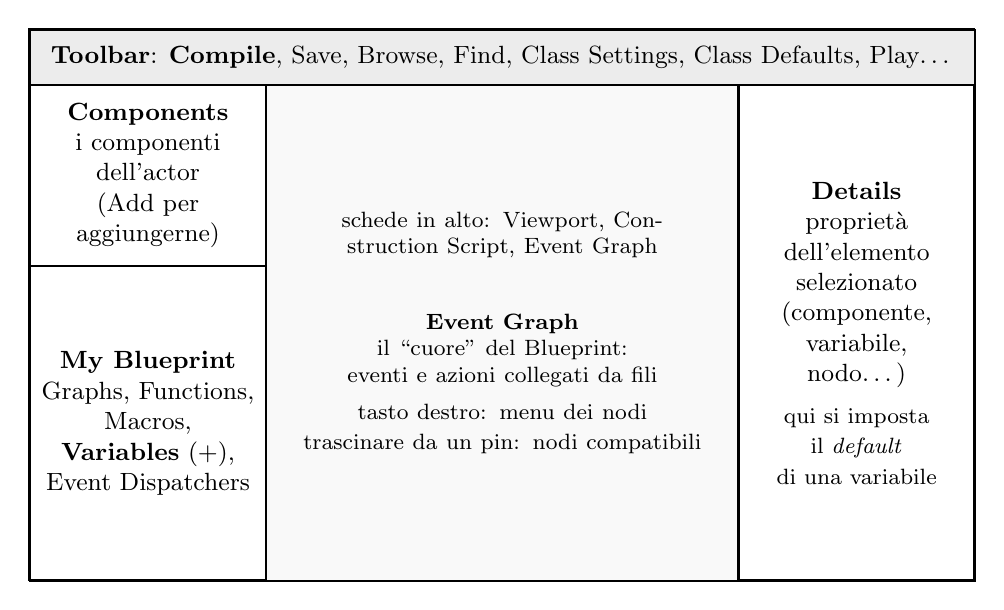
\begin{tikzpicture}[
  font=\small,
  ue2pan/.style={draw, thick, align=center, inner sep=3pt}
]
  \draw[thick] (0,0) rectangle (12,7);
  \node[ue2pan, minimum width=12cm, minimum height=0.7cm, anchor=north west,
    fill=gray!15] at (0,7) {\textbf{Toolbar}: \textbf{Compile}, Save, Browse, Find,
    Class Settings, Class Defaults, Play\ldots};
  \node[ue2pan, minimum width=3cm, minimum height=2.3cm, anchor=north west]
    at (0,6.3) {\textbf{Components}\\i componenti\\dell'actor\\(Add per\\aggiungerne)};
  \node[ue2pan, minimum width=3cm, minimum height=4cm, anchor=north west]
    at (0,4.0) {\textbf{My Blueprint}\\Graphs, Functions,\\Macros,\\
    \textbf{Variables} (+),\\Event Dispatchers};
  \node[ue2pan, minimum width=6cm, minimum height=6.3cm, anchor=north west,
    text width=5.6cm, fill=gray!5] at (3,6.3) {\footnotesize schede in alto:
    Viewport, Construction Script, Event Graph\\[18pt]\textbf{Event Graph}\\il ``cuore'' del Blueprint:\\
    eventi e azioni collegati da fili\\[4pt]\footnotesize tasto destro: menu dei nodi\\
    \footnotesize trascinare da un pin: nodi compatibili};
  \node[ue2pan, minimum width=3cm, minimum height=6.3cm, anchor=north west]
    at (9,6.3) {\textbf{Details}\\proprietà\\dell'elemento\\selezionato\\
    (componente,\\variabile,\\nodo\ldots)\\[4pt]\footnotesize qui si imposta\\
    \footnotesize il \emph{default}\\\footnotesize di una variabile};
\end{tikzpicture}
\caption{L'editor dei Blueprint (Blueprint Class Editor), ricostruito dalla lezione e
dal primo capitolo del libro di Romero e Sewell. La disposizione dei pannelli si può
cambiare, come nel Level Editor.}
\label{ue2:fig:editorbp}
\end{figure}

\paragraph{Approfondimento: i pannelli dell'editor.} Romero e Sewell, nel primo capitolo,
elencano i pannelli principali del \emph{Blueprint Class Editor}: la
\textbf{Toolbar}, i \textbf{Components} (i componenti già pronti che si aggiungono con
Add: \emph{mesh} statiche, luci, suoni, collisioni, particelle, camere), \textbf{My
Blueprint} (dove si creano variabili, macro, funzioni e grafi, con i pulsanti +), i
\textbf{Details} (le proprietà dell'elemento selezionato, con una barra di ricerca in
alto), la \textbf{Viewport} e l'\textbf{Event Graph}. Nell'Event Graph, notano gli
autori, un \textbf{evento} è un nodo \textbf{rosso}, e le altre azioni che seguono un
evento si collegano con dei fili; ci si sposta nel grafo trascinando con il tasto
destro. Di ogni evento se ne può mettere \textbf{uno solo} per grafo, ma si possono
creare eventi propri (\textbf{Add Custom Event}). Oltre a BeginPlay e Tick, il libro
cita gli eventi di \textbf{collisione} (quando due actor si scontrano o si
sovrappongono), gli eventi di \textbf{input} (tastiera, mouse, \emph{touch},
\emph{gamepad}) ed \textbf{Event End Play}, quando l'actor sta per essere rimosso.

% ---------------------------------------------------------------------
\section{Il primo nodo: Print String}
\label{ue2:sec:print}

``Andremo a fare una piccola prova.'' Unreal gestisce tutto con i \textbf{nodi}. Se si
porta il mouse sul ``pinnetto'' bianco a forma di freccia dell'Event BeginPlay, lo si
clicca e lo si \textbf{trascina verso l'esterno}, al rilascio compare un menu con tutti
i blocchi che si possono collegare: ``possiamo metterci tutto quello che vogliamo, tutti
i blocchi che ci serviranno per fare un'azione''.

\paragraph{Print String.} L'azione più semplice è \textbf{Print String}, che
``letteralmente ci stampa qualcosa a schermo''. Il testo predefinito è ``Hello''.

\paragraph{La barra ``Development Only''.} Igor fa notare un dettaglio. A differenza di
altri nodi, come \textbf{Set Actor Location} o \textbf{Enable Collision}, il Print String
ha una \textbf{barra in basso}. Vuol dire che quel blocco ha effetto \textbf{solo in
modalità di sviluppo}: quando si sviluppa e si va in Play nell'editor funziona, ma se si
facesse un \textbf{eseguibile} da mandare a qualcun altro ``questa cosa non avverrà
mai''. Gli altri nodi, invece, sì.

\paragraph{Compilare.} ``Molto importante'': quando si fanno dei cambiamenti
importanti bisogna \textbf{compilare} (\textbf{Compile}, in alto a sinistra). La
compilazione ``legge quello che abbiamo fatto'' e aggiorna il programma; in molti casi
Unreal lo fa anche in automatico, ma conviene farlo sempre. E \textbf{salvare},
``ovviamente, sempre buona cosa''.

\paragraph{La prova.} Si abbassa la finestra del Blueprint, si \textbf{mette l'actor
nella scena} (``ovviamente, se no non succede niente'': il Blueprint è solo una classe,
finché non se ne mette una copia nel livello non esiste) e si preme Play. In alto a
sinistra compare ``Hello'', ma per pochissimo. Igor cambia allora il parametro
\textbf{Duration} del nodo a 100 secondi, e la scritta resta: ``è piccolo'', ma c'è.
L'actor è entrato in funzione e ha fatto la sua azione appena ha cominciato a esistere,
cioè subito, perché era già nella scena.

\paragraph{Una finestra di gioco separata.} ``Se vi è più comodo'', si può far partire il
gioco in una finestra esterna: dai \textbf{tre puntini} accanto al pulsante Play si
sceglie \textbf{New Editor Window (PIE)}. ``Io lo trovo molto più comodo'': invece di
abbassare e rialzare la finestra del Blueprint, il gioco gira in una finestra a parte da
cui si controlla tutto. Igor lo scrive anche in chat.

\paragraph{Approfondimento: \emph{development} e \emph{shipping}.} La barra del Print
String rimanda a una distinzione che Romero e Sewell spiegano nel capitolo sul
\emph{packaging}: le \emph{build} di \textbf{sviluppo} (\emph{Development}) contengono
informazioni che servono al \emph{debug}, quelle di \textbf{distribuzione}
(\emph{Shipping}) sono più ``pulite'', senza informazioni di \emph{debug}, e sono quelle
da pubblicare. I nodi marcati \emph{Development Only}, come il Print String, vengono
semplicemente ignorati in una \emph{build} Shipping: si possono quindi lasciare nel
grafo mentre si lavora senza che il giocatore finale veda mai le scritte di prova.

% ---------------------------------------------------------------------
\section{Le variabili: GET e SET, colori e calcoli}
\label{ue2:sec:variabili}

\paragraph{Che cos'è una variabile.} Igor chiede chi abbia mai sentito parlare di
variabili \emph{bool}, \emph{float}, \emph{int}; qualcuno sì. Una \textbf{variabile} è
``uno slot di una tipologia di valore'' in cui si può mettere un valore: ``è come una
\textbf{scatola}''. Si creano delle piccole scatoline in cui mettere dei valori, ma ogni
scatola è fatta per un certo contenuto: ``c'è la scatola per i gioielli, c'è la scatola
per le praline'' (``mi invento un po' di cose''). Il tipo della variabile decide che cosa
ci si può mettere dentro.

\paragraph{Creare una variabile.} L'esempio: rendere ``esterna'' la durata del Print
String, cioè metterla in una variabile. Nel pannello My Blueprint, alla voce
\textbf{Variables}, si clicca \textbf{+}: si crea subito una variabile, di tipo booleano
oppure dello stesso tipo dell'ultima variabile creata. Igor la chiama \textbf{duration
time text}\footnote{Così nella trascrizione (una volta ``duration time next''); il nome
esatto digitato non si sente, ma non ha importanza per l'esempio.}.

\paragraph{GET e SET.} Se si trascina la variabile nel grafo, Unreal chiede se si vuole
un \textbf{GET} o un \textbf{SET}. GET è \textbf{prendere} il valore che c'è dentro; SET
è \textbf{impostare} il valore dentro. Per dare il valore alla durata del Print String
serve un GET.

\paragraph{I colori devono combaciare.} ``Però attenzione, che succede? Questo è rosso e
questo è verde.'' Il pin della variabile appena creata è \textbf{rosso} (è una
booleana), quello della Duration è \textbf{verde}: ``non sono della stessa tipologia''.
Due pin rossi si collegano; un rosso e un verde no. Il verde è il \textbf{float}. ``Cosa
sono i numeri float?'' ``I numeri con la virgola.'' ``Ottimo'': i numeri con i
\textbf{decimali}. Si cambia quindi il tipo della variabile in Float, il pin diventa
verde, e ``guardate un po', si collega''.

\paragraph{\emph{Please compile the Blueprint}.} Appena collegata, la variabile mostra
l'avviso \emph{please compile the blueprint}: è stata appena creata, e il Blueprint ``non
sa ancora che c'è una variabile nuova''. Dopo la compilazione, nei Details compare il
suo \textbf{valore predefinito} (\emph{Default Value}): ``guarda, questo è il tuo valore.
Quanto lo vuoi?'' Igor mette 10. In Play la scritta dura 10 secondi (``un po' tanti'') e
poi scompare: ``non è più 100''. La lezione: si possono creare variabili, impostarle e
darle ai blocchi di esecuzione.

\paragraph{Nodi di esecuzione e nodi di calcolo.} I \textbf{blocchi di esecuzione} si
riconoscono perché hanno l'intestazione \textbf{blu} e il pin di esecuzione, ``la
freccettina'' bianca. Ci sono però anche nodi \textbf{verdi} senza quel pin: sono nodi
che ``\textbf{calcolano solamente}''. Igor ne fa vedere uno, \textbf{Find Look at
Rotation}: chiede due variabili di un tipo e ne restituisce un'altra, dello stesso tipo
o di un altro. ``Oppure, esempio classico'': gli \textbf{operatori} aritmetici, il
\textbf{+}, il \textbf{$-$} (\emph{Subtraction}), il \textbf{per}, che si cerca con
l'\textbf{asterisco} (\emph{Multiply}), e il \textbf{diviso} (\emph{Divide}). Si
possono invocare tutti gli operatori che servono (figura~\ref{ue2:fig:pin}).

\paragraph{Sottrarre due secondi.} L'esempio: ``indipendentemente da quanto tempo noi
mettiamo qua dentro'', togliere sempre 2 secondi. Si prende il nodo meno, si collega la
variabile al primo ingresso (il nodo ``è diventato verde'', perché ha riconosciuto che si
tratta di un float, e ``ci chiede: te lo sottraggo di un altro float''), si scrive 2 nel
secondo e si collega il risultato alla Duration.

\paragraph{Da numero a testo.} Si può anche \textbf{stampare} il valore: collegando il
float all'ingresso di testo del Print String, Unreal inserisce in automatico un
\textbf{convertitore}. I pin \textbf{rosa} sono le \textbf{stringhe}, cioè testo. In
Play, il Print String non stampa più ``Hello'' ma \textbf{8}, ``che è 10 meno 2'', e la
scritta dura 8 secondi. (Ogni volta che Igor apre Unreal, Zoom va a scatti: ``a quanto
pare mi lagga Zoom benissimo''.)

\begin{figure}[htbp]
\centering
\begin{tikzpicture}[
  font=\small,
  ue2node/.style={draw, thick, rounded corners=4pt, align=center},
  ue2exec/.style={-{Stealth[length=2.5mm]}, very thick},
  ue2flt/.style={-{Stealth[length=2mm]}, thick, green!50!black},
  ue2str/.style={-{Stealth[length=2mm]}, thick, magenta}
]
  \node[ue2node, fill=red!15, minimum width=2.6cm, minimum height=1.2cm]
    (bp) at (0,0) {\textbf{Event}\\\textbf{BeginPlay}};
  \node[ue2node, fill=blue!10, minimum width=3.4cm, minimum height=2.6cm,
    anchor=north west] (pr) at (7.4,0.6) {};
  \node[font=\small\bfseries, anchor=north] at (pr.north) {Print String};
  \node[font=\footnotesize, anchor=west] (ins) at (7.5,-0.5) {In String};
  \node[font=\footnotesize, anchor=west] (dur) at (7.5,-1.2) {Duration};
  \node[font=\scriptsize\itshape, anchor=south] at (pr.south) {Development Only};
  \node[ue2node, fill=green!10, minimum height=0.8cm] (get) at (0.4,-1.9)
    {GET duration (float)};
  \node[ue2node, fill=green!10, minimum height=0.8cm] (minus) at (3.6,-1.9)
    {$x - 2$};
  \node[ue2node, fill=magenta!8, minimum height=0.8cm, font=\footnotesize]
    (conv) at (5.6,-0.5) {float $\to$ string};
  \draw[ue2exec] (bp.east) -- node[above, font=\footnotesize]{esecuzione}
    (bp.east -| pr.west);
  \draw[ue2flt] (get) -- (minus);
  \draw[ue2flt] (minus.east) -- ++(0.4,0) |- (dur.west);
  \draw[ue2flt] (minus.north) |- (conv.west);
  \draw[ue2str] (conv.east) -- (ins.west);
\end{tikzpicture}
\caption{Il primo grafo della lezione, nella sua versione finale: all'inizio del gioco
l'actor stampa la durata meno 2 (cioè 8) per 8 secondi. La freccia nera è il filo di
\textbf{esecuzione} (l'ordine delle azioni, da sinistra a destra); le frecce colorate
sono fili di \textbf{dati}, del colore del loro tipo (verde il float, rosa la stringa).
Il nodo blu, con il pin di esecuzione, è un'\textbf{azione}; i nodi verdi, senza, sono
nodi di \textbf{calcolo}, che si eseguono quando un'azione chiede il loro valore. Il
convertitore è inserito da Unreal in automatico. Schema ricostruito, non copia della
schermata.}
\label{ue2:fig:pin}
\end{figure}

% ---------------------------------------------------------------------
\section{Primo esercizio: Time To Print}
\label{ue2:sec:esercizio1}

``Vorrei fare un piccolo esercizio con voi. Molto velocissimo.''

\paragraph{Staccare un filo.} Prima, un comando: per \textbf{staccare} un collegamento
si tiene premuto \textbf{Alt} e si clicca sul pin.

\paragraph{La consegna.} Creare un'altra variabile, \textbf{time to print}, di tipo
\textbf{float}; staccare la variabile della durata dall'ingresso del testo e collegarci
invece time to print; dare a time to print il valore \textbf{5}, che dovrà essere
stampato a schermo. Anche la Duration va messa a 5. ``Senza che andiamo a vedere poi
ognuno'': l'importante è che ognuno dica ``stampa 5, sì''.

\paragraph{Un esercizio guidato.} Uno studente arriva in ritardo (``scusate, non
riuscivo ad entrare''). A una studentessa il Print String stampa \textbf{0}, e Igor la
guida passo per passo in condivisione dello schermo: fermare il gioco (lo
\textbf{Stop}, o il tasto \textbf{Esc}); creare la variabile dal \textbf{+} di Variables
nel pannello a sinistra; chiamarla time to print; cambiarle il tipo per farla
\textbf{verde}, cioè float (``bravissima''); prenderne il GET; staccare il vecchio
collegamento con Alt e attaccare time to print; compilare (``in alto a sinistra'');
poi, con la variabile selezionata, guardare nei \textbf{Details} a destra: ``vedi, adesso
è apparsa. In fondo''. In fondo ai Details c'è il \textbf{valore predefinito}, ed è lì
che si mette il 5. Lo 0 dipendeva proprio da questo: il valore predefinito di un float
appena creato è zero.

% ---------------------------------------------------------------------
\section{I dettagli di una variabile, e il \emph{tuning}}
\label{ue2:sec:dettagli}

Tutte le caratteristiche di una variabile si vedono nei \textbf{Details}, sia cliccando
la variabile nel grafo, sia cliccandola nella lista Variables. Igor consiglia di
impostare l'engine \textbf{in inglese} (``io sono più abituato all'inglese''), ma se si
trova più facile l'italiano non c'è nessun problema.

\paragraph{Il nome, il tipo, la descrizione.} Nei Details si possono cambiare il nome, il
tipo e una \textbf{descrizione}. La descrizione non la vedrà il giocatore, ma ``i nostri
amici programmatori, o comunque colleghi'': ci si può scrivere un piccolo commento,
come ``variabile da stampare nel Print''. È un'informazione ``per lo più organizzativa'',
``non un qualcosa che troverete spesso''.

\paragraph{Pubblica e privata: Instance Editable.} L'opzione \textbf{Instance Editable}
rende una variabile \textbf{pubblica}. Gli studenti non conoscono la distinzione ``in
questo contesto''. Una variabile \textbf{privata} esiste solo all'interno dell'actor;
una \textbf{pubblica} si può vedere e modificare direttamente nei \textbf{Details}
dell'actor piazzato nel livello. Uno studente chiede se sia come ``globale e locale''.
``Non esattamente, perché globale è anche un'altra cosa che andremo a vedere'': le
variabili davvero globali si fanno con la \textbf{Game Instance}, un oggetto che
\textbf{esiste finché esiste il gioco} e che può contenere variabili da ``dare in pasto''
a tutti gli actor che si vuole.

\paragraph{L'occhietto.} Lo stesso risultato si ottiene con l'icona
dell'\textbf{occhio} accanto alla variabile nella lista. Igor lo mostra: con l'occhio
aperto, selezionando l'actor nel livello, nei Details compare la sezione
\textbf{Default} con \emph{time to print}; con l'occhio chiuso, dopo aver ricompilato,
la voce scompare.

\paragraph{Il \emph{tuning}.} A che cosa serve? ``Il design è sempre con me.'' Come
designer, a Igor è capitato spesso di fare \textbf{\emph{tuning}}: la pratica di
\textbf{aggiustare i valori}, ``quanto danno fa, quanto fa di contrattacco'', in
generale i valori modificabili. Diceva al programmatore: ``lasciami quei valori, che li
devo controllare'', cioè testare. E poi andava nei Details dell'actor e cambiava
``questo, quell'altro, questo, quell'altro''. Le variabili pubbliche servono proprio a
questo: permettono di \textbf{interagire con l'editor stesso} senza toccare il grafo. Le
cose private, invece, restano nel campo dell'actor.

\paragraph{Approfondimento: gli attributi di una variabile.} Romero e Sewell, nel secondo
capitolo, elencano tutti gli attributi che i Details mostrano per una variabile.
\begin{itemize}
  \item \textbf{Variable Name} e \textbf{Variable Type}: il nome e il tipo. I Blueprint
        sono un linguaggio \textbf{fortemente tipizzato}: il tipo si sceglie alla
        creazione e non cambia durante l'esecuzione.
  \item \textbf{Instance Editable}: se attivo, \textbf{ogni copia} del Blueprint
        piazzata nel livello può avere un valore diverso; altrimenti tutte le copie
        (le \emph{istanze}) condividono lo stesso valore iniziale. È la precisazione
        tecnica del ``pubblico'' di Igor.
  \item \textbf{Blueprint Read Only}: se attivo, i nodi non possono modificare la
        variabile.
  \item \textbf{Tooltip}: il testo che compare passando il mouse sulla variabile; è la
        ``descrizione'' di cui parla Igor.
  \item \textbf{Expose on Spawn}: la variabile si può impostare nel momento in cui
        l'actor viene \emph{spawnato}.
  \item \textbf{Private}: se attivo, i Blueprint figli non possono modificarla.
  \item \textbf{Expose to Cinematics}: la rende visibile al Sequencer.
  \item \textbf{Category}: per raggruppare le variabili.
  \item \textbf{Slider Range} e \textbf{Value Range}: il minimo e il massimo, per lo
        \emph{slider} e per i valori ammessi. Per il \emph{tuning} sono preziosi: chi
        aggiusta i valori non può uscire dai limiti sensati.
  \item \textbf{Replication}: per i giochi in rete.
  \item \textbf{Default Value}: il valore iniziale; si può impostare solo dopo aver
        compilato, come si è visto nell'esercizio.
\end{itemize}

% ---------------------------------------------------------------------
\section{I tipi di variabile}
\label{ue2:sec:tipi}

Igor cancella tutto (seleziona e preme \textbf{Canc}, \emph{Delete} sulla tastiera
inglese) e passa a una slide sui tipi di variabile (tabella~\ref{ue2:tab:tipi}).
``Immaginiamoci sempre delle scatolette, con dentro dei valori.''

\paragraph{Booleana.} ``Qualcuno ha mai sentito parlare di booleane?'' Qualche sì,
qualche no. Una variabile \textbf{booleana} ha due valori possibili: \textbf{vero} o
\textbf{falso}. ``Dentro o c'è vero, o c'è falso, una delle due. Basta.'' Con un esempio
dall'elettrotecnica, è ``letteralmente lo \emph{switch} della luce'': spento è falso,
acceso è vero; a livello di circuito, ``è aperto o è chiuso''.

\paragraph{Byte, Integer, Integer64.} Il \textbf{byte} è un valore numerico intero
compreso tra 0 e 255. L'\textbf{integer}\footnote{Nella trascrizione ``gli integrali, i
numeri integrali''.}, o intero, è un numero \textbf{senza la virgola}: ``1, 2, 3, 4, 5,
6, 7, 8, senza virgola, senza niente'', compreso tra $-2^{31}$ e $2^{31}$ (``possiamo
anche non capire qual è il numero preciso, perché tanto è difficile che ci arriviamo'').
L'\textbf{integer64} arriva a 64 bit, tra $-2^{63}$ e $2^{63}$.

\paragraph{Float.} Il \textbf{float} è il valore numerico \textbf{con i decimali}.

\paragraph{Name, String, Text.} Il \textbf{name} è un testo usato principalmente per gli
\textbf{identificatori}, per identificare degli elementi in Unreal. La \textbf{string}
è un gruppo di caratteri \textbf{alfanumerici}, ``numeri e lettere''. Uno studente chiede
la differenza: anche il name è una stringa? La stringa, risponde Igor, si usa per lo più
nei \textbf{testi}; i name sono \textbf{nomenclature}: ``il nome di un livello, il nome
di un \emph{asset}''. ``Tipo un'etichetta'', propone lo studente: ``bravissimo, è come
un'etichetta'', ``quasi come un \textbf{tag}''. Il \textbf{text}, infine, è un testo
usato principalmente nella \textbf{UI}, la \emph{user interface}: tutto ciò che è 2D e
con cui l'utente interagisce, un termine usato ``in tanti campi, anche coi siti''.

\paragraph{Vector, Rotator, Transform.} I \textbf{vettori} sono ``molto importanti'',
essendo Unreal un ambiente tridimensionale. Un vettore può essere la
\textbf{locazione}: ``ci ricordiamo che quando abbiamo spostato i nostri cubetti e coni
abbiamo visto quei tre valori cambiare, la X, la Y e la Z?'' Un vettore è ``la
composizione'' di questi tre: una variabile che contiene \textbf{tre valori}, X, Y e Z.
Il \textbf{rotator} contiene gli X, Y e Z della \textbf{rotazione} (``poi faremo un po'
di discorsi, perché esistono i quaternioni, eccetera''). Il \textbf{transform}
contiene location, rotation e scala.

\paragraph{Object.} Infine il tipo \textbf{object}: ``volendo, noi potremmo creare una
variabile di tipologia di un actor che abbiamo creato''. È una variabile che contiene un
\textbf{riferimento} a un actor (si vedrà con il Level Blueprint,
sezione~\ref{ue2:sec:level}).

\begin{table}[htbp]
\centering
\small
\begin{tabular}{@{}p{2.2cm}p{2.0cm}p{8.8cm}@{}}
\toprule
\textbf{Tipo} & \textbf{Colore} & \textbf{Che cosa contiene} \\
\midrule
Boolean & rosso & vero o falso (\emph{true}/\emph{false}) \\
Byte & verde scuro & intero da 0 a 255 (8 bit) \\
Integer & verde acqua & intero da $-2^{31}$ a $2^{31}-1$ (32 bit) \\
Integer64 & verde acqua scuro & intero da $-2^{63}$ a $2^{63}-1$ (64 bit) \\
Float & verde & numero con decimali; in Unreal Engine 5 i Blueprint lo trattano in
  precisione singola o doppia (\emph{Double}) \\
Name & lilla & identificatore, ``etichetta'' (nome di un livello, di un \emph{asset}) \\
String & rosa & gruppo di caratteri alfanumerici \\
Text & rosa scuro & testo per la UI, \textbf{localizzabile} (traducibile) \\
Vector & giallo & tre float X, Y, Z (per esempio una locazione) \\
Rotator & viola-lilla & tre float della rotazione: X (\emph{roll}), Y (\emph{pitch}),
  Z (\emph{yaw}) \\
Transform & arancione & locazione, rotazione e scala \\
Object & blu & riferimento a un oggetto (per esempio un actor nel livello) \\
\bottomrule
\end{tabular}
\caption{I tipi di variabile della slide di Igor, con i colori dei loro pin
nell'editor (i nomi dei colori sono approssimativi) e le integrazioni del libro di
Romero e Sewell (i limiti esatti degli interi, \emph{roll}, \emph{pitch} e \emph{yaw},
la localizzazione del Text).}
\label{ue2:tab:tipi}
\end{table}

\paragraph{Approfondimento: Double, Text e i tre angoli.} Tre precisazioni dal secondo
capitolo del libro. Primo: oltre al Float a 32 bit (sette cifre decimali di
precisione) esiste il \textbf{Double} a 64 bit (sedici cifre); in Unreal Engine 5 l'editor
mostra entrambi come ``Float'' e sceglie la precisione da solo. Secondo: il
\textbf{Text} serve ai testi che saranno \textbf{localizzati}, cioè tradotti in altre
lingue: è per questo che è il tipo della UI, mentre String è il testo ``di servizio'' e
Name l'identificatore. Terzo: i tre valori del \textbf{Rotator} hanno un nome. X è il
\textbf{\emph{roll}} (il rollio, la rotazione attorno all'asse X, quello ``in avanti''),
Y il \textbf{\emph{pitch}} (il beccheggio, attorno all'asse Y, alzare o abbassare il
muso), Z lo \textbf{\emph{yaw}} (l'imbardata, attorno all'asse Z verticale, girare a
destra e a sinistra). Sono i nomi che compariranno nei nodi della piattaforma
(sezione~\ref{ue2:sec:mouse}). I \textbf{quaternioni} a cui accenna Igor sono un altro
modo, matematicamente più robusto, di rappresentare una rotazione: evitano il problema
del \emph{gimbal lock}, in cui due dei tre assi finiscono per coincidere e si perde un
grado di libertà. Unreal li usa al suo interno, ma nei Blueprint si lavora quasi sempre
con i Rotator.

% ---------------------------------------------------------------------
\section{Le booleane e il Branch}
\label{ue2:sec:branch}

``Adesso vi faccio vedere.'' Igor crea una variabile, la chiama ``letteralmente''
\textbf{bool}, e le dà il tipo booleano.

\paragraph{GET e SET in un gesto.} ``Piccola cosetta'': invece di scegliere dal menu, si
può fare un GET ``velocissimamente'' trascinando la variabile nel grafo con
\textbf{Ctrl} premuto, e un SET trascinandola con \textbf{Alt}. Il \textbf{GET} è il pin
che dice ``questa è la scatoletta che c'è dentro qualcosa, prendi il valore da qui''. Il
\textbf{SET} è diverso: ha un \textbf{nodo di esecuzione}, a differenza del GET, e ha una
\textbf{casella di spunta}\footnote{Nella trascrizione ``un TIL'': è il \emph{tick},
la spunta della casella.}: cliccandola si imposta il valore. ``Col SET sto letteralmente
impostando il suo valore'': spunta, vero; niente spunta, falso.

\paragraph{Stampare una booleana.} Igor rifà un Print String con Duration 10 (``sennò è
troppo poco''), collega il pin della booleana al testo e va in Play: in alto a sinistra
compare \textbf{false}. Mette la spunta, rifà Play: \textbf{true}. Il Print String
riceve, tramite la stringa, il valore della variabile.

\paragraph{A che cosa serve sapere se è vero o falso?} ``La domanda magari è: ok, ma che ci
serve?'' Serve perché si possono usare delle \textbf{condizioni}. ``Qualcuno ha mai
sentito parlare di \emph{if}, \emph{else}?'' Edoardo sì: ``ho studiato informatica alle
superiori''. ``Grande, perfetto.'' L'\textbf{if-else} è una condizione, e in Unreal non si
chiama così: tenendo premuto \textbf{B} e cliccando nel grafo compare il
\textbf{Branch}, ``cioè due percorsi''. È ``un \textbf{bivio}'': ``se questa condizione
che abbiamo qua è vera, vai per questo percorso; se questa condizione è falsa, vammi per
un altro''.

\paragraph{Il primo Branch.} Igor collega il Branch dopo il BeginPlay e porta la
variabile bool nel pin rosso \textbf{Condition}. Sull'uscita \textbf{True} mette un Print
String con ``la variabile è vera''; per l'uscita \textbf{False} copia il nodo (``per
copiare qualcosa, Ctrl+C, Ctrl+V, classico'') e scrive ``la variabile è falsa''. Con la
variabile falsa, in Play esce ``la variabile è falsa''; con la spunta, ``la variabile è
vera'' (figura~\ref{ue2:fig:branch}).

\paragraph{I binari del treno.} ``Letteralmente sta prendendo un bivio: o vado di qua, o
vado di là.'' Igor lo paragona ai \textbf{binari di un treno}: ``se la leva è a destra,
vado a destra; se la leva è a sinistra, vado a sinistra. E la nostra leva è la nostra
variabile''. Il bool è molto importante perché permette di avere delle condizioni, e
quindi gli attori ``\textbf{pensano}'': hanno la ``capacità di scelte'', ``ah, ok, allora
prendo questa strada perché ho questa variabile di questo tipo''.

\begin{figure}[htbp]
\centering
\begin{tikzpicture}[
  font=\small,
  ue2node/.style={draw, thick, rounded corners=4pt, align=center,
                  minimum height=1cm},
  ue2exec/.style={-{Stealth[length=2.5mm]}, very thick},
  ue2bool/.style={-{Stealth[length=2mm]}, thick, red!70!black}
]
  \node[ue2node, fill=red!15, minimum width=2.4cm] (bp) at (0,0)
    {\textbf{Event}\\\textbf{BeginPlay}};
  \node[ue2node, fill=gray!10, minimum width=2.2cm, minimum height=1.6cm]
    (br) at (4,0) {\textbf{Branch}\\[2pt]\footnotesize Condition};
  \node[ue2node, fill=green!8, minimum width=1.6cm] (get) at (1.6,-1.8) {GET bool};
  \node[ue2node, fill=blue!10, text width=3.6cm] (pt) at (9,0.9)
    {\textbf{Print String}\\\footnotesize ``la variabile è vera''};
  \node[ue2node, fill=blue!10, text width=3.6cm] (pf) at (9,-0.9)
    {\textbf{Print String}\\\footnotesize ``la variabile è falsa''};
  \draw[ue2exec] (bp) -- (br);
  \draw[ue2bool] (get.east) -| ([xshift=-4mm]br.south);
  \draw[ue2exec] ([yshift=4mm]br.east) -- node[above, font=\footnotesize]{True}
    ++(1.2,0) |- (pt.west);
  \draw[ue2exec] ([yshift=-4mm]br.east) -- node[below, font=\footnotesize]{False}
    ++(1.2,0) |- (pf.west);
\end{tikzpicture}
\caption{Il Branch è un bivio: segue l'uscita True o l'uscita False a seconda del valore
della condizione. ``La nostra leva è la nostra variabile.''}
\label{ue2:fig:branch}
\end{figure}

\paragraph{Si può accedere al codice?} Uno studente chiede se sia possibile accedere anche
al codice, ``immagino che sia C''. Sì, è possibile, ``però non lo faremo''. Con il C++ si
possono definire anche i blocchi stessi, creare blocchi di tipo diverso; ma ``di base, su
Blueprint possiamo farlo allo stesso modo anche noi''. Chi vuole può andare a vederlo; e
c'è chi va ``proprio nel profondo della programmazione'', come gli \emph{engine
programmer}.

\paragraph{Allineare i nodi.} ``Una piccola cosa, se vi piace l'ordine'': si selezionano
due nodi e si preme \textbf{Q}, e Unreal li allinea.

\paragraph{Approfondimento: Branch e operatori relazionali.} Romero e Sewell presentano il
Branch nel secondo capitolo, parlando del \textbf{percorso di esecuzione}: i pin bianchi
sono i \textbf{pin di esecuzione}, gli altri, colorati, i \textbf{pin di dati};
l'esecuzione parte da un evento rosso e segue il filo bianco da sinistra a destra fino
all'ultimo nodo. Alcuni nodi, come il Branch, \textbf{controllano il flusso}: decidono
quale strada prendere. Il loro esempio è un personaggio con una booleana \emph{Has
Shield}: se è vera, il Branch imposta \emph{Shield Value} a 100; se è falsa, a 0. Nella
lezione la condizione è sempre una variabile booleana; nella pratica, spesso, è il
risultato di un \textbf{operatore relazionale}: i nodi $<$, $\leq$, $>$, $\geq$, $=$,
$\neq$ confrontano due valori e restituiscono una booleana. L'esempio del libro: quando
un oggetto subisce danni, un Branch controlla se \emph{Health} $\leq 0$, e in quel caso
l'oggetto viene distrutto; se no, non succede niente, perché all'uscita False non è
collegato nulla. Quanto alla scorciatoia: nel menu che si apre con il tasto destro su
una selezione di nodi c'è la voce \textbf{Alignment}, con allineamenti in alto, al
centro, in basso, a sinistra, a destra, e \textbf{Straighten Connection(s)}, che
raddrizza i fili; il tasto \textbf{Q} è la scorciatoia di quest'ultima. Il libro ricorda
anche le altre scorciatoie ``tasto + clic'': \textbf{B} per il Branch, \textbf{S} per il
nodo Sequence, \textbf{D} per il Delay, \textbf{F} per il For Each Loop
(tabella~\ref{ue2:tab:scorciatoie}).

% ---------------------------------------------------------------------
\section{Gli operatori logici: AND, OR, NOT}
\label{ue2:sec:logici}

Igor cancella i nodi di prova (``tanto non ci sono problemi'') e passa agli
\textbf{operatori logici}. ``Qualcuno ha mai sentito parlare di AND, OR, NOT?'' Sì.

\paragraph{Il gioco dei tubi.} A che cosa servono? Una variabile booleana ha i suoi valori,
vero e falso; ``però mettiamo conto che ne abbiamo altre'', e bisogna metterle in
\textbf{comparazione}. L'esempio è ``il gioco dei tubi'', l'enigma in cui bisogna girare i
tubi nel verso giusto per collegarli. Se ci sono due tubi, per risolvere l'enigma un tubo
deve essere girato nel modo giusto \textbf{e} anche l'altro: sono \textbf{due
condizioni} da prendere insieme. ``Come facciamo a metterle insieme?''

\paragraph{I nodi.} Igor crea una seconda booleana, \textbf{bool 2}. Gli operatori si
cercano scrivendo \textbf{OR Boolean}, \textbf{AND Boolean} e \textbf{NOT Boolean}.
``Questi sono i tre più usati''; ce ne sono altri, come il NOR, ``ma sono un attimo da
vedere poi più avanti''.

\paragraph{OR.} L'OR dice: ``se almeno un valore è vero, allora la condizione finale è
vera''. Con bool vera e bool 2 falsa, collegato alla condizione del Branch, esce ``la
variabile è vera''. È ``un modo per sommare le variabili tra \emph{true} e \emph{false}'',
``una specie di somma, chiamiamola così'': ``letteralmente dice: o questa, o questa''.

\paragraph{AND.} L'AND, con gli stessi valori, vero e falso, dà ``la variabile è falsa'',
``perché AND vuol dire \emph{questa e questa}'': tutte le condizioni devono essere vere
perché il risultato sia vero. Igor mette vera anche la seconda e\ldots{} non succede
niente: ``scusate, questo non l'ho collegato, sono io''. Collegato, esce ``la variabile è
vera''. Ricapitolando: se tutte e due sono vere, è vero; se una sola è falsa, ``tutto
quanto è falso''; se tutte e due sono false, è falso (``doppio falso'').

\paragraph{NOT.} Il NOT ha un solo ingresso e ``letteralmente \textbf{inverte}'': se la
variabile è vera diventa falsa, se è falsa diventa vera. Collegato a una variabile vera,
dà falso. ``Non lo useremo tanto.'' La tabella~\ref{ue2:tab:logici} riassume i tre
operatori.

\begin{table}[htbp]
\centering
\small
\begin{tabular}{@{}cc|ccc|ccc@{}}
\toprule
\textbf{A} & \textbf{B} & \textbf{A OR B} & \textbf{A AND B} & \textbf{NOT A} &
  \textbf{A NOR B} & \textbf{A NAND B} & \textbf{A XOR B} \\
\midrule
falso & falso & falso & falso & vero  & vero  & vero  & falso \\
falso & vero  & vero  & falso & vero  & falso & vero  & vero  \\
vero  & falso & vero  & falso & falso & falso & vero  & vero  \\
vero  & vero  & vero  & vero  & falso & falso & falso & falso \\
\bottomrule
\end{tabular}
\caption{Le tabelle di verità degli operatori logici. Le prime tre colonne di risultati
sono gli operatori della lezione; le ultime tre sono un'integrazione dal libro di Romero
e Sewell.}
\label{ue2:tab:logici}
\end{table}

\paragraph{Approfondimento: NOR, NAND, XOR, e perché l'OR è una ``somma''.} Il libro
completa la lista degli operatori logici dei Blueprint con tre combinazioni. Il
\textbf{NOR} (NOT + OR) è vero solo se entrambi gli ingressi sono falsi; il \textbf{NAND}
(NOT + AND) è falso solo se entrambi sono veri; lo \textbf{XOR}, l'OR esclusivo, è vero
se i due ingressi sono \textbf{diversi}. L'esempio del libro per l'AND: un Print String
che si esegue solo se \emph{Health} $> 70$ \textbf{e} \emph{Shield Value} $> 50$, con
due operatori relazionali che alimentano un AND. Quanto alla ``somma'' di Igor, è
un'intuizione che ha un nome: nell'\textbf{algebra di Boole}, da cui il tipo
\emph{boolean} prende il nome, l'OR si scrive come una somma ($A + B$) e l'AND come un
prodotto ($A \cdot B$). Se si leggono vero e falso come 1 e 0, l'AND si comporta
esattamente come una moltiplicazione (basta uno 0 per fare 0), e l'OR come una somma
in cui ``1 + 1'' resta 1.

% ---------------------------------------------------------------------
\section{Secondo esercizio: due Branch, OR e AND}
\label{ue2:sec:esercizio2}

``Allora facciamo un piccolo esercizio.''

\paragraph{La consegna.} All'Event BeginPlay si collega un \textbf{SET} della variabile
bool (quello che si ottiene trascinandola con Alt), e il suo valore va alla condizione
di un \textbf{primo Branch}. Su ciascuna uscita del primo Branch va un \textbf{secondo
Branch}: su True un Branch la cui condizione è \textbf{bool OR bool 2}; su False un
Branch la cui condizione è \textbf{bool AND bool 2}. Solo se il secondo Branch è vero si
stampa, e invece di ``la variabile è vera'' si stampa \textbf{il valore finale} del
calcolo, collegando l'uscita dell'operatore all'In String
(figura~\ref{ue2:fig:esercizio2}). ``Ce la fate?'' Cinque minuti.

\begin{figure}[htbp]
\centering
\begin{tikzpicture}[
  font=\small,
  ue2node/.style={draw, thick, rounded corners=4pt, align=center,
                  minimum height=0.9cm},
  ue2exec/.style={-{Stealth[length=2.5mm]}, very thick},
  ue2bool/.style={-{Stealth[length=2mm]}, thick, red!70!black}
]
  \node[ue2node, fill=red!15] (bp) at (0,0) {\textbf{BeginPlay}};
  \node[ue2node, fill=blue!10] (set) at (2.6,0) {\textbf{SET bool}\\\footnotesize
    $\square$ / $\checkmark$};
  \node[ue2node, fill=gray!10] (b1) at (5.2,0) {\textbf{Branch 1}\\\footnotesize
    cond.\ = bool};
  \node[ue2node, fill=gray!10] (b2) at (8.4,1.5) {\textbf{Branch 2}};
  \node[ue2node, fill=gray!10] (b3) at (8.4,-1.5) {\textbf{Branch 3}};
  \node[ue2node, fill=green!8] (or) at (8.4,3.1) {bool \textbf{OR} bool 2};
  \node[ue2node, fill=green!8] (and) at (8.4,-3.1) {bool \textbf{AND} bool 2};
  \node[ue2node, fill=blue!10, text width=2.3cm] (p1) at (11.6,1.5)
    {\textbf{Print}\\\footnotesize risultato OR};
  \node[ue2node, fill=blue!10, text width=2.3cm] (p2) at (11.6,-1.5)
    {\textbf{Print}\\\footnotesize risultato AND};
  \draw[ue2exec] (bp) -- (set);
  \draw[ue2exec] (set) -- (b1);
  \draw[ue2exec] (b1.east) ++(0,0.2) -- ++(0.5,0) |- node[pos=0.75, above,
    font=\footnotesize]{True} (b2.west);
  \draw[ue2exec] (b1.east) ++(0,-0.2) -- ++(0.5,0) |- node[pos=0.75, below,
    font=\footnotesize]{False} (b3.west);
  \draw[ue2bool] (or) -- (b2);
  \draw[ue2bool] (and) -- (b3);
  \draw[ue2exec] (b2) -- node[above, font=\footnotesize]{True} (p1);
  \draw[ue2exec] (b3) -- node[below, font=\footnotesize]{True} (p2);
  \draw[ue2bool, dashed] (or.east) -| (p1.north);
  \draw[ue2bool, dashed] (and.east) -| (p2.south);
\end{tikzpicture}
\caption{Il secondo esercizio. Le frecce nere sono l'esecuzione, quelle rosse i valori
booleani (tratteggiate: il risultato dell'operatore, convertito in testo e stampato). Le
uscite False dei Branch 2 e 3 non sono collegate: in quei casi non si stampa niente.}
\label{ue2:fig:esercizio2}
\end{figure}

\paragraph{Le domande durante l'esercizio.} Lo studente arrivato in ritardo chiede come
si crea il Print String: tasto destro, Print String. Un altro si è perso gli operatori:
si scrivono proprio ``AND Boolean'', ``OR Boolean'', ``NOT Boolean''. Una studentessa non
ricorda come si prende ``l'oggetto con il pallino rosso'' (la variabile): ``mettilo qua
dentro, ti appare in automatico''. Trascinando la variabile direttamente sul pin, Unreal
crea da solo il GET.

\paragraph{La spunta che non c'entra.} Un'altra studentessa ha un problema: sul primo
Branch, nella condizione, ha una \textbf{spunta} che Igor non ha. Il pin Condition non è
collegato all'\textbf{uscita} del SET. ``Devi collegare questo pallino a questo
pallino.'' Igor spiega che cosa è successo, con una dimostrazione. Il nodo SET ha a
destra un pin di uscita: ``è il valore che io gli ho impostato'', che esce dal nodo
``come un collegamento''. Il Branch ha a sinistra ``un posto in cui posso mettere quel
valore''. Se il pin non è collegato, la casella di spunta del Branch è una
\textbf{condizione interna al Branch}, che non ha niente a che vedere con la variabile:
``la porta si aprirà secondo bool, non secondo questa condizione qua''. Igor mette la
variabile a vero e la spunta del Branch a falso: il Print String collegato al True
``non mi stampa niente'', ``perché questa qua non è relativa a questa''. Collegando il
pin, stampa. (``Stavo impazzendo perché non mi stampava niente.'')

\paragraph{I ``what if''.} Poi Igor cerca ``un candidato'' per una piccola verifica:
``se io adesso vi cambio un po' i parametri, dove andiamo a finire con tutte le linee?''
Si offre uno studente.
\begin{itemize}
  \item \textbf{bool vero, bool 2 falso.} ``Siccome è \emph{true}, finisce sopra, sul
        primo Branch'' (il Branch 2 della figura). ``Controlla se tra bool e bool 2 uno
        dei due è vero. In questo caso lo è, perché hai settato bool come vero. Il
        secondo non è importante.'' Quindi va su True e stampa il valore. ``Perfetto.
        Netto, liscio.''
  \item \textbf{bool falso.} ``False scende giù e controlla se entrambi, bool e bool 2,
        sono veri. In questo caso bool è falso, quindi anche qui il secondo valore non
        è importante, perché uno dei due è falso. Il risultato dell'AND è falso e non
        stampa niente.'' ``Esatto, perfetto.''
\end{itemize}
La morale: ``indipendentemente dalle condizioni, possiamo cambiare i binari di un
percorso di programmazione''. È ``una delle cose più principali'', e serve molto spesso
per \textbf{diversificare i comportamenti} dei Blueprint. Igor chiede ancora se ci sono
domande, e decide di non cancellare il grafo ma di lasciarlo lì, scollegato. ``Sono stato
chiaro, dai.''

\paragraph{Approfondimento: la valutazione ``pigra''.} Lo studente coglie, senza
nominarlo, un principio importante: in un OR, se il primo ingresso è vero il secondo
``non è importante''; in un AND, se il primo è falso il secondo non cambia il risultato.
In molti linguaggi di programmazione questo si chiama \emph{short-circuit evaluation}
(valutazione a corto circuito): il secondo operando non viene nemmeno calcolato. Nei
nodi Blueprint, attenzione, i due ingressi vengono comunque calcolati entrambi; ma il
ragionamento sul \emph{risultato} è lo stesso, ed è quello che serve per prevedere dove
andrà l'esecuzione.

% ---------------------------------------------------------------------
\section{Il Level Blueprint e la piattaforma}
\label{ue2:sec:level}

``Adesso andremo a fare una piccola cosa direttamente nel nostro bellissimo Blueprint.''
L'obiettivo è una \textbf{piattaforma} che \textbf{ruota}, cioè si inclina, ``a seconda
di quanto premiamo'' dei tasti (D, A, e così via).

\paragraph{La piattaforma.} Si prende un \textbf{cubo} dal pannello Place Actors, lo si
mette in scena e lo si allarga ``quanto volete'', fino a farne una piattaforma.

\paragraph{Il Level Blueprint.} ``Vi farò conoscere il bellissimo mondo del \textbf{Level
Blueprint}.'' In Unreal esiste anche un Blueprint \textbf{interno al livello}: quando si
apre quel livello, al suo interno ci sono delle regole (``spawna qualcosa'', eccetera).
Lo si apre dall'icona dei Blueprint nella barra in alto: \textbf{Open Level Blueprint}.
Una studentessa si è persa (``scusa, come lo apriamo?''), e Igor le mostra l'icona.

\paragraph{Un evento di input.} Si è parlato di eventi con le loro condizioni; uno dei più
semplici è l'\textbf{input}. Tasto destro nel grafo, si scrive \textbf{W} e si sceglie
la voce con ``l'immaginetta della tastierina'' e la W: è un evento che scatta
\textbf{alla pressione del tasto W}.

\paragraph{La referenza.} Ma come si dice al grafo che deve agire su \emph{quella}
piattaforma? Si crea una \textbf{referenza}. Con il cubo selezionato nel livello, nel
Level Blueprint si fa tasto destro e si sceglie \textbf{Create a Reference to Cube94}
(il cubo di Igor si chiama Cube94, e lo si ritrova con quel nome nell'Outliner). ``Questo
può essere fatto solo nel Level Blueprint, ve lo dico.''

\paragraph{Set Actor Rotation e i suoi pin.} Dalla referenza si trascina un filo e si
sceglie \textbf{Set Actor Rotation}. Il nodo ha tre pin di dati:
\begin{itemize}
  \item un pin \textbf{blu}, il \textbf{Target}: un \emph{Actor Object Reference}, cioè
        una variabile che si riferisce a un actor, a uno qualunque degli elementi della
        \emph{viewport}, ``che abbiano programmazione o meno''. È l'actor su cui il nodo
        agisce;
  \item un pin \textbf{lilla}, \textbf{New Rotation}: un \textbf{rotator}, la
        composizione degli assi X, Y e Z della rotazione;
  \item un pin \textbf{rosso}, un \textbf{bool}: \textbf{Teleport} (tornerà utile con
        la fisica, sezione~\ref{ue2:sec:fisica}).
\end{itemize}

\paragraph{Il Player Start.} Per vedere la piattaforma serve un punto da cui partire.
``Prendete il \textbf{Player Start}'': lo si trova nel Place Actors, o cercandolo, ed è
``un controllone'' (l'icona di un \emph{joystick}). Lo si mette davanti alla piattaforma
e lo si gira verso di essa.

\paragraph{Consume Input.} Selezionando l'evento W, nei Details c'è una casella
interessante, \textbf{Consume Input}. Se è spuntata, il tasto W ``sarà dedicato solo a
questo evento'': il giocatore non potrà più usarlo per muoversi in avanti. Senza la spunta
si muoverebbe ``avanti e indietro''; ``a noi interessa stare fermi'', quindi la spunta
resta.

\paragraph{Quale asse, e in che verso.} La piattaforma va ruotata attorno all'asse
\textbf{X}. In positivo o in negativo? Igor lo verifica nella \emph{viewport} ruotando il
cubo: in un verso la rotazione è negativa, nell'altro positiva. ``Per come mi regolo'',
W manda la piattaforma in avanti, quindi si piega in un verso, e indietro nell'altro.
Igor scrive 5 nella X del New Rotation e prova.

% ---------------------------------------------------------------------
\section{La mobilità: Static, Stationary, Movable}
\label{ue2:sec:mobilita}

Non funziona, ``giustamente'', e Unreal mostra un avviso: ``ricordate che questo che mi è
appena uscito è un problema che Unreal ci darà sempre''. L'actor non ha la capacità di
essere \textbf{Movable}: non si può muovere nel mondo.

\paragraph{Dove si trova.} Nel \emph{transform} dell'actor, sotto location, rotation e
scala, c'è la \textbf{Mobility}, con tre valori: \textbf{Static}, \textbf{Stationary} e
\textbf{Movable}. È ``la tipologia di oggetto'' rispetto a come reagisce al mondo, e
riguarda ``soprattutto il rendering''.
\begin{itemize}
  \item \textbf{Static.} L'oggetto sa che non si muoverà. Quando si calcolano le luci,
        la sua ombra viene calcolata una volta e poi è come \textbf{dipinta}: ``è
        dipinta''. ``Per alleggerirsi la cosa'', l'engine dice: è un oggetto statico,
        ``basta che mi calcolo una volta l'ombra e basta''.
  \item \textbf{Stationary.} Una via di mezzo: le ombre vengono messe in
        \emph{cache}\footnote{Nella trascrizione ``vengono chesciate'': con ogni
        probabilità ``cachate'', dall'inglese \emph{cached}.}, l'oggetto può essere
        cambiato, ma non può essere mosso.
  \item \textbf{Movable.} Totalmente \textbf{dinamico}.
\end{itemize}
La piattaforma va messa su \textbf{Movable}, e allora ruota di 5 gradi. Igor prova con
valori più grandi (``facciamo tipo 25'') per vederlo meglio.

\paragraph{Approfondimento: la mobilità secondo il libro.} Romero e Sewell incontrano lo
stesso problema nel quinto capitolo, quando un bersaglio cilindrico deve cominciare a
muoversi: bisogna prima portare la sua Mobility da Static a \textbf{Movable}, nei Details
sotto il TRANSFORM. E aggiungono una nota importante: gli actor di base piazzati nel
mondo sono \textbf{Static per impostazione predefinita}, e gli oggetti statici sono
``significativamente meno costosi'' da renderizzare; per questo Static dovrebbe essere
la scelta predefinita per tutto ciò che non è interattivo, per tenere alto il
\emph{frame rate}. Stationary ha senso soprattutto per le \textbf{luci}: una luce
Stationary non si sposta, ma se ne possono cambiare colore e intensità durante il gioco,
e parte della sua illuminazione è precalcolata. Movable va riservato agli oggetti che
devono davvero muoversi.

% ---------------------------------------------------------------------
\section{Ruotare di 5 gradi a ogni pressione: Split Struct Pin}
\label{ue2:sec:split}

\paragraph{Funziona una volta sola.} ``Però che succede? Guardate un po'.'' Se si preme
di nuovo W, la piattaforma non fa niente. Il problema è che la si sta impostando a un
\textbf{valore preciso}: Set Actor Rotation dice ``mettiti a 25 gradi'', e la seconda
volta la piattaforma risponde ``ci sto già, a 25''. Serve invece una rotazione che
\textbf{parta da quella attuale}.

\paragraph{Prendere i valori dell'actor.} Igor mostra che dalla referenza di un actor si
possono prendere \textbf{tutti} i suoi valori: la location, la rotation, la scala, la
\emph{mesh}, i materiali (``che poi vedremo''). ``È andare nella scatola di
quell'\emph{asset}'': prendo quel valore, e poi lo modifico. Qui serve \textbf{Get Actor
Rotation}, la rotazione attuale, ``che si aggiorna ogni volta''.

\paragraph{Split Struct Pin.} La rotazione è data da tre valori, X, Y e Z, e se ne vuole
modificare uno solo. Con il tasto destro sul pin del Rotator si sceglie \textbf{Split
Struct Pin}: il pin si divide nei suoi tre valori, ``e guardate un po', la cosa bella è
che sono cambiati di colore''. Sono diventati \textbf{verdi}, ``perché sono tre valori
float''. Uno studente chiede come si fa a trovare i tre valori; Igor rifà il gesto
all'indietro (\textbf{Recombine Struct Pin}) e poi di nuovo avanti: tasto destro, Split
Struct Pin. Si fa lo stesso sul pin New Rotation del Set Actor Rotation, che altrimenti,
lilla, non accetterebbe un float.

\paragraph{Il grafo.} Si prende la X di Get Actor Rotation, le si somma 5 con un nodo
\textbf{+}, e il risultato va nella X del Set Actor Rotation
(figura~\ref{ue2:fig:piattaforma}, a sinistra). Ora la piattaforma si inclina di 5 gradi
a ogni pressione di W: ``posso aggiungere quanto me ne pare'', a parte che a un certo
punto la piattaforma \textbf{compenetra} il pavimento. ``Prima non andava bene e adesso
invece sì'', perché ogni volta si parte dalla rotazione attuale. Con un Print String
collegato alla X, a ogni pressione compaiono i valori \textbf{0, 5, 10, 15, 20, 25, 30,
35}: ``si aumenta sempre''.

\begin{figure}[htbp]
\centering
\begin{tikzpicture}[
  font=\small,
  ue2node/.style={draw, thick, rounded corners=4pt, align=center,
                  minimum height=0.9cm},
  ue2exec/.style={-{Stealth[length=2.5mm]}, very thick},
  ue2flt/.style={-{Stealth[length=2mm]}, thick, green!50!black},
  ue2obj/.style={-{Stealth[length=2mm]}, thick, blue!70!black}
]
  % versione prima della pausa
  \node[font=\footnotesize\bfseries] at (2.6,2.2) {Prima della pausa};
  \node[ue2node, fill=red!15] (w) at (0,1.2) {\textbf{W}\\\footnotesize Pressed};
  \node[ue2node, fill=blue!10, text width=3.2cm] (set) at (4.6,1.2)
    {\textbf{Set Actor Rotation}\\\footnotesize New Rotation (split)};
  \node[ue2node, fill=blue!5] (ref) at (0,-0.6) {Cube94};
  \node[ue2node, fill=green!8, text width=2.0cm] (get) at (2.0,-1.9)
    {\textbf{Get Actor Rotation}\\\footnotesize (split)};
  \node[ue2node, fill=green!8] (plus) at (4.6,-0.6) {X $+\,5$};
  \draw[ue2exec] (w) -- (set);
  \draw[ue2obj] (ref.east) -- ++(0.4,0) |- (get.west);
  \draw[ue2obj] (ref.north) -- ++(0,0.3) -| ([xshift=-12mm]set.south);
  \draw[ue2flt] (get.east) -| (plus.south);
  \draw[ue2flt] (plus) -- (set);
  % separatore
  \draw[gray, dashed] (7.2,2.4) -- (7.2,-2.6);
  % versione dopo la pausa
  \node[font=\footnotesize\bfseries] at (10.2,2.2) {Dopo la pausa};
  \node[ue2node, fill=red!15] (w2) at (8.4,1.2) {\textbf{W}};
  \node[ue2node, fill=blue!10, text width=3.2cm] (add) at (11.8,1.2)
    {\textbf{Add Actor World}\\\textbf{Rotation}\\\footnotesize Delta Rotation: X $= 5$};
  \node[ue2node, fill=blue!5] (ref2) at (8.4,-0.6) {Cube94};
  \node[ue2node, fill=red!15] (s2) at (8.4,-1.9) {\textbf{S}};
  \node[ue2node, fill=blue!10, text width=3.2cm] (add2) at (11.8,-1.6)
    {\textbf{Add Actor World}\\\textbf{Rotation}\\\footnotesize X $= -5$};
  \draw[ue2exec] (w2) -- (add);
  \draw[ue2exec] (s2) -- (add2);
  \draw[ue2obj] (ref2.east) -- ++(0.5,0) |- ([yshift=-2mm]add.west);
  \draw[ue2obj] (ref2.east) -- ++(0.5,0) |- ([yshift=2mm]add2.west);
\end{tikzpicture}
\caption{La piattaforma comandata da tastiera, nel Level Blueprint. A sinistra la prima
versione: si legge la rotazione attuale, si aggiungono 5 gradi alla X e la si reimposta.
A destra la versione adottata dopo la pausa: Add Actor World Rotation aggiunge
direttamente 5 gradi (o $-5$) alla rotazione, nello spazio del mondo. A e D funzionano
allo stesso modo sull'asse Y.}
\label{ue2:fig:piattaforma}
\end{figure}

% ---------------------------------------------------------------------
\section{Il problema di Giulia, e la pausa}
\label{ue2:sec:problema}

``Un attimo, un attimo.'' A Giulia la piattaforma si muove \textbf{una volta sola}. Igor
segue il problema in condivisione dello schermo, e il \emph{debug} dal vivo è istruttivo anche
perché non arriva a una risposta.
\begin{itemize}
  \item La piattaforma è \textbf{Movable}? Sì.
  \item Il grafo è uguale a quello di Igor? Sembra di sì: Cube71 (il suo cubo), Set
        Actor Rotation, il più, il Get Actor Rotation. Ruotata a mano con E nella
        \emph{viewport}, la piattaforma ruota normalmente.
  \item Forse un problema di \textbf{collisioni} con il pavimento? Igor fa alzare la
        piattaforma: niente.
  \item Igor fa rifare alcuni collegamenti, ricostruire il nodo, splittarlo di nuovo,
        eliminare un nodo superfluo (``questo get actor\ldots{} l'actor location
        sopra?'', ``è uguale, lo elimino''), ricollegare il Target al Cube71. Niente.
  \item La \textbf{camera}: Giulia vede ``la piattaforma sbilenca e basta''. Igor fa
        girare il Player Start di 90 gradi e mettere la piattaforma davanti. Niente.
  \item Ha cliccato nella finestra di gioco, perché riceva l'input? Sì, ``solo una
        volta''. Il Consume Input c'è.
  \item Un controllo più fine: Igor chiede di selezionare il nodo Set Actor Rotation e
        premere \textbf{F9}, che vi mette un \emph{breakpoint}. In Play il nodo viene
        effettivamente raggiunto: ``funziona a meraviglia''. Eppure la piattaforma non
        ruota oltre la prima volta.
  \item Infine Giulia si accorge che nel livello \textbf{manca il Player Start}
        (``mancano delle robe che ho cercato di mettere, ma ho perso''). Igor fa
        rimettere il Player Start dal Place Actors.
\end{itemize}
A quel punto è ora della pausa: ``facciamo pausa, io intanto cerco di capire un po' il
problema che c'è, Giulia''. Venti minuti.

\paragraph{La soluzione, durante la pausa.} Durante la pausa Igor prova una cosa diversa:
al posto di Set Actor Rotation, con il Get e il più, usa \textbf{Add Actor World
Rotation}, con la referenza come Target e 5 nella X (``senza il più, senza niente, solo
questi due''; $-5$ per la S, che Giulia non ha ancora). ``Sì, adesso lo fa. Perfetto.''
``Ma era un errore mio?'' ``No, no, tranquillo.'' La spiegazione di Igor è che il problema
dipende dagli assi: con Set Actor Rotation si stava ruotando ``sulla sua relativa'', ed è
meglio ruotare sull'asse \textbf{globale}, quello del mondo. Ma su un punto Igor è
onesto: ``il fatto che non prenda l'input a ogni W, quello non te lo so dire, perché a
tutti quanti lo prendeva''. ``Non so se magari è un \emph{flash} o un qualcosa, non ne ho
idea. Ti devo dire la verità.'' Per capirlo dovrebbe guardare con calma le impostazioni
dell'editor di Giulia; intanto si semplifica. ``Visto che ho risolto la cosa, vado a farmi il
caffè'', dice Giulia. ``Ottima idea. Pure io.''

\paragraph{Approfondimento: Set, Add Local, Add World, e il \emph{breakpoint}.} Unreal ha
più nodi per ruotare un actor, e la differenza è esattamente quella tra assi locali e
globali vista nella prima lezione.
\begin{itemize}
  \item \textbf{Set Actor Rotation} imposta una rotazione \textbf{assoluta}: ``mettiti
        così''. Per ottenere un incremento bisogna leggere la rotazione attuale e
        sommarci qualcosa, come nella prima versione.
  \item \textbf{Add Actor Local Rotation} aggiunge una rotazione attorno agli assi
        \textbf{locali} dell'actor, quelli che ruotano con lui.
  \item \textbf{Add Actor World Rotation} aggiunge una rotazione attorno agli assi
        \textbf{del mondo}, che restano fissi: premere W inclina sempre la piattaforma
        ``in avanti'' rispetto alla scena, comunque sia già inclinata.
\end{itemize}
Perché la prima versione non funzionasse sul computer di Giulia la lezione non lo
stabilisce, e il capitolo non è in grado di dirlo; il passaggio sul nodo ``get actor
location'' da eliminare fa pensare a un collegamento sbagliato (la \emph{location},
gialla, al posto della \emph{rotation}, lilla), ma è solo un'ipotesi. Resta istruttivo
il metodo. Il \textbf{\emph{breakpoint}} (F9 su un nodo selezionato) ferma l'esecuzione
quando il gioco arriva a quel nodo e apre l'editor del Blueprint lì, mostrando i valori
che passano nei fili: è il modo più diretto per sapere se un nodo viene davvero eseguito
e con quali dati. Lo stesso F9 lo toglie. Il Print String, che Igor usa per tutta la
lezione, è l'altro strumento: stampa i valori a schermo senza fermare il gioco.

% ---------------------------------------------------------------------
\section{Dopo la pausa: Add Actor World Rotation e i tasti W A S D}
\label{ue2:sec:wasd}

``Ora ci siamo, ragazzi?'' Visto il problema di Giulia, Igor semplifica l'esercizio per
tutti, con il blocco che ha usato durante la pausa: \textbf{Add Actor World Rotation},
``nel senso che andiamo semplicemente a mettere una rotazione nel mondo, non dipendente
dalla sua relatività''. Prima, spiega, si impostava la rotazione relativa all'asse
dell'actor; doveva essere relativa al mondo. La consegna: tenere solo i due blocchi
(l'evento e Add Actor World Rotation), levare tutto il resto, \textbf{splittare} il pin
della rotazione e scrivere 5 nella X (figura~\ref{ue2:fig:piattaforma}, a destra).
``Praticamente qui si dovrebbe tranquillamente muovere, molto più semplice.''

\paragraph{S, A e D.} Igor ha aggiunto anche la \textbf{S}: ``se una è 5, l'altra è
$-5$''. E per destra e sinistra, A e D? ``Su che asse ci dobbiamo muovere?'' Lo si vede
nella \emph{viewport}: cliccando la piattaforma e guardando il gizmo, se W e S ruotano
attorno alla X, A e D devono ruotare attorno alla \textbf{Y}. ``E vorrei questo piccolo
esercizio: lo fate voi.'' A e D, ``non è Donkey Kong, questo con la tastiera''. ``Mi
raccomando, ricordatevi sempre che il \textbf{Target} è importante'': senza collegarlo, il
nodo non si riferisce a niente.

\paragraph{Allineare in verticale?} Uno studente chiede se esista un tasto per allineare i
blocchi in verticale. ``Non lo conosco, devo dire la verità.'' (L'allineamento c'è, nel
menu Alignment del tasto destro: si veda l'approfondimento della
sezione~\ref{ue2:sec:branch}.)

\paragraph{Qual è il verso di D?} Un altro studente non capisce che valore mettere sulla
D. Igor lo guarda insieme a lui sulla piattaforma: destra, nella sua vista, è ``di là'',
opposto a lui. Ruotando a mano la piattaforma in quel verso, il valore che compare sulla
Y è negativo: ``siccome siamo in asse globale, devi andare in negativo sulla Y''. La
soluzione, ``velocissimamente, perché se no non abbiamo tempo'': gli stessi due blocchi,
il Target collegato, la rotazione sulla Y, $+5$ per un tasto e $-5$ per l'altro. ``E
possiamo, wow, destra e sinistra.''

% ---------------------------------------------------------------------
\section{La pallina, la fisica e il Teleport}
\label{ue2:sec:fisica}

``Qua sopra, una bella sferetta.'' In Unreal gli oggetti possono essere
\textbf{fisici}. Si prende una \textbf{sfera} dal Place Actors e la si mette sulla
piattaforma. In Play, però, ``quella rimane lì, sta lì ferma'': ``non gliene frega
assolutamente nulla''. La sua fisica non è attiva.

\paragraph{Simulate Physics.} Nei Details della sfera c'è la casella \textbf{Simulate
Physics}. Spuntata, in Play la sfera \textbf{cade} e rotola: ``abbiamo la nostra sferetta
che si muove''. Uno studente chiede dove si attiva: basta cliccare la sfera e cercare la
voce. Un altro condivide lo schermo: ``una cosa che va, finalmente''.

\paragraph{La pallina scagliata.} C'è però una cosa particolare: muovendo la
piattaforma, la sfera viene \textbf{scagliata in alto}, oltre a uscire dai bordi. Che
esca si risolve ``semplicemente mettendoci un muro, un muro invisibile'' (lo si farà alla
fine, sezione~\ref{ue2:sec:vaschetta}). Che venga lanciata, invece, dipende dal modo in
cui la piattaforma si muove.

\paragraph{La freccia sotto il nodo, e il Teleport.} Nel Level Blueprint, sotto il nodo
Add Actor World Rotation c'è una \textbf{freccia}: cliccandola si aprono altri parametri.
``Molto spesso blocchi del genere hanno queste tipologie di parametri interni, che sono
nascosti un po'.'' Uno è \textbf{Teleport}. La spiegazione di Igor: quando c'è uno
spostamento nello spazio, l'engine lo fa avvenire sui \emph{tick}, sui \emph{frame}, e
``pum!'': lo spostamento porta con sé il \textbf{fattore fisico}, ``abbiamo proprio là il
colpo fisico'', che spinge via la pallina. Se invece lo si \textbf{teletrasporta}, ``è
come fare un \emph{pop-up}'' dello spostamento della piattaforma: l'effetto fisico si
annulla, e la pallina non viene scaricata via. Igor abbassa un po' la pallina, spunta
Teleport su tutti i nodi e va in Play: ``la nostra palletta non verrà influenzata dalla
particolarità fisica della nostra piattaforma''.

\paragraph{Approfondimento: che cosa fa davvero Teleport.} Quando Unreal sposta o ruota
un oggetto che partecipa alla simulazione fisica, deve decidere come trattare quel
movimento. Con \textbf{Teleport} disattivato, lo spostamento è considerato un movimento
``vero'': il motore fisico ricava dalla differenza tra la posizione vecchia e quella
nuova una \textbf{velocità}, e la trasmette agli oggetti a contatto. Una piattaforma che
ruota di 5 gradi in un solo \emph{frame} ha, per il motore fisico, una velocità enorme,
e la pallina riceve un colpo proporzionato. Con \textbf{Teleport} attivo, lo spostamento
è un salto istantaneo, senza velocità associata: la pallina si ritrova sulla piattaforma
nella nuova posizione e scivola per gravità, senza essere colpita. Accanto a Teleport,
nella stessa sezione nascosta, c'è spesso \textbf{Sweep}: se attivo, l'oggetto si ferma
quando nel tragitto incontra qualcosa che lo blocca, invece di attraversarlo.

\paragraph{I bug della fisica.} Mentre gli studenti provano, uno trova ``un \emph{bug}'':
se si porta la pallina in un angolo e si premono insieme W e A, cioè le direzioni
opposte all'angolo, la pallina \textbf{finisce sotto} la piattaforma. (Un altro nota che
E porta il giocatore in alto e Q in basso: anche durante il gioco ci si muove come
nell'editor.) Igor risponde che ``possono esserci dei \emph{bug} fisici'', perché la
\textbf{fisica è emergente}: spostare le cose con la fisica dipende da come la si
gestisce, e ``probabilmente ne potresti trovare non pochi''. Ci sono engine proprietari,
``come quello di Valve'', che gestiscono fisica e gravità ``in un modo assurdo'', ``con
molto matematichese'', e sono ottimizzati per le azioni che quei giochi fanno. Unreal,
``essendo più generico come sistema fisico'', può dare problemi fisici ``molto più
evidenti, molto più spesso''.

\paragraph{``Non va niente''.} Uno studente ha messo anche la S, ma premendo W, A, S, D
non succede niente. Igor gli fa cliccare la piattaforma: non è \textbf{Movable}. ``È la
terza'' delle tre opzioni. Rimessa su Movable, funziona; manca solo il Teleport.

\paragraph{Approfondimento: il motore fisico di Unreal.} Unreal Engine 5 usa un motore
fisico proprio, \textbf{Chaos}, che ha sostituito PhysX della quarta versione. È pensato
per essere generale: corpi rigidi, distruzione, tessuti, veicoli. Il caso della pallina
che finisce sotto la piattaforma ha un nome, \textbf{\emph{tunneling}}: se in un
\emph{frame} un oggetto si sposta più dello spessore di ciò che dovrebbe fermarlo, il
motore fisico non vede mai il contatto e l'oggetto ``passa attraverso''. Con il Teleport
attivo la piattaforma salta da una rotazione all'altra senza che la fisica la segua, e
il rischio aumenta. Le difese tipiche sono oggetti più spessi, spostamenti più piccoli a
ogni \emph{frame} e la \textbf{CCD} (\emph{Continuous Collision Detection}), un'opzione
dei componenti fisici che controlla le collisioni lungo tutto il tragitto e non solo
nelle posizioni finali.

% ---------------------------------------------------------------------
\section{L'Event Tick e i \emph{delta seconds}}
\label{ue2:sec:tick}

``Abbiamo il nostro bellissimo gioco della palla incredibile.'' Il passo successivo è
comandare la piattaforma con il \textbf{mouse} invece che con W A S D. Prima, però, un
evento nuovo.

\paragraph{Che cos'è un tick.} ``Sapete cos'è un \emph{tick}?'' È, semplicemente,
``\textbf{un per \emph{frame}}''. L'\textbf{Event Tick} è un blocco che esegue tutto ciò
che c'è dopo di lui \textbf{a ogni \emph{frame}}: ``ogni \emph{tick}, ogni \emph{tick},
ogni \emph{frame}''.

\paragraph{La piattaforma che gira da sola.} Igor copia un Add Actor World Rotation,
collega la referenza come sempre e lo attacca all'Event Tick: 5 gradi a ogni
\emph{frame}. ``Non sto premendo nulla'', e la piattaforma gira da sola, velocissima.
Quanti sono gli \emph{fps}? ``In questo caso saranno tipo 100'': la piattaforma ruota di 5
gradi cento volte al secondo.

\paragraph{I \emph{delta seconds}.} L'Event Tick ha un'uscita, \textbf{Delta Seconds}:
``l'intervallo tra un \emph{frame} e l'altro''. Perché la velocità sia la stessa
``indipendentemente dal numero di \emph{frame}'' (30, 60, 70, 100), bisogna
\textbf{moltiplicare} il valore per i \emph{delta seconds}. Si tira fuori un
\textbf{Multiply}, si collega Delta Seconds e si scrive 5. ``Vedete, è molto diverso da
prima'': la piattaforma gira molto più piano. Prima si aggiungevano 5 gradi a ogni
\emph{frame}; ora si moltiplica il tempo tra i \emph{frame} per 5. E se il gioco
girasse a 30, 60, 70, 100, 120 o 144 \emph{fps}, la velocità sarebbe la stessa; senza la
moltiplicazione, con un limite a 30 \emph{fps} sarebbe più lenta che a 100.

\paragraph{``Un tick ogni 5 frame?''} Uno studente prova a riformulare: ``quindi in realtà
non fa partire il programma ogni 5 \emph{tick}, ma fa in modo che un \emph{tick} sia ogni
5 \emph{frame}?'' ``Non 5 \emph{frame}: 5 \textbf{unità}'', le unità in cui si muove la
piattaforma; ``è il float, fondamentalmente''. Il \emph{tick} resta uno per
\emph{frame}; cambia quanto si muove l'oggetto a ogni \emph{tick}.

\paragraph{La regola.} ``Questa è una cosa da tenere tanto a mente, soprattutto con
oggetti che si muovono.'' Se in un progetto si fa un oggetto in movimento senza
\emph{delta seconds}, ``vi si ritorcerà contro'': su una macchina con certe prestazioni
andrà più lento, su un'altra più veloce. ``Moltiplicatevi i \emph{delta seconds} se
muovete le cose, soprattutto nel tempo.'' Per il gioco della pallina, però, la rotazione
continua non serve, ``perché se no non ha \emph{gameplay}'': ``sarebbe quasi un
mulino''.

\paragraph{Approfondimento: i conti.} Con i numeri di Igor: senza \emph{delta seconds},
5 gradi per \emph{frame} a 100 \emph{fps} fanno $5 \times 100 = 500$ gradi al secondo,
quasi un giro e mezzo; a 30 \emph{fps} ne fanno 150. Con i \emph{delta seconds}, a 100
\emph{fps} ($\Delta t = 0{,}01$~s) ogni \emph{frame} aggiunge $5 \times 0{,}01 = 0{,}05$
gradi, a 30 \emph{fps} ($\Delta t \approx 0{,}033$~s) circa $0{,}167$: in un secondo, in
entrambi i casi,
\[
  \sum_{\text{frame in 1 s}} 5 \cdot \Delta t = 5 \cdot 1~\text{s} = 5~\text{gradi}.
\]
Il 5, insomma, non è più ``gradi per \emph{frame}'' ma \textbf{gradi al secondo}: è la
``unità'' di cui parla Igor rispondendo allo studente. Romero e Sewell, nel secondo
capitolo, descrivono l'Event Tick proprio così (a 60 \emph{frame} al secondo viene
chiamato 60 volte al secondo) e, nel quinto, usano lo stesso prodotto velocità $\times$
\emph{delta time} per muovere un bersaglio. Più avanti, presentando i
\textbf{timer}, il libro li indica come alternativa all'Event Tick: tutto ciò che si
collega al Tick viene eseguito a ogni \emph{frame}, e ciò che non ha bisogno di
aggiornarsi così spesso può essere eseguito a intervalli più lunghi.

% ---------------------------------------------------------------------
\section{La piattaforma comandata dal mouse}
\label{ue2:sec:mouse}

``Adesso sto staccando tutto, stacco tutto quanto. Voglio dare il movimento al mio
mouse.''

\paragraph{Evento o valore.} Per il mouse ci sono due cose diverse con lo stesso nome.
C'è l'\textbf{evento} \textbf{Mouse X}, che scatta ``quando ho un input dal mouse X'', e
c'è il \textbf{valore} \textbf{Get Mouse X}, ``proprio il valore del mouse X''. Mouse X
è il movimento del mouse a destra e a sinistra (Mouse Y, in alto e in basso). Invece di
usare un evento, Igor fa ``molto più semplice'': resta sull'Event Tick, collega
\textbf{Get Mouse X} al \textbf{Roll} (la X della rotazione) e \textbf{Get Mouse Y} al
\textbf{Pitch} (la Y) dell'Add Actor World Rotation. La piattaforma si muove con il
mouse; ``è molto incontrollabile'', ma si muove.

\paragraph{Assi scambiati, e invertiti.} I due valori risultano scambiati, ``perché
dipende dalla \emph{world location}'', da come è orientata la piattaforma rispetto al
mondo: si invertono X e Y, ``ed è molto meglio''. Poi c'è il verso. A Igor non piace
che, portando il mouse in giù, la piattaforma si pieghi in quel modo: ``lo vogliamo fare
al contrario''. ``Qualcuno ha qualche idea per invertire un valore? In matematica, come
si inverte un valore in negativo?'' ``Moltiplichi per meno 1.'' ``Bravissimo.'' Si prende
Get Mouse X, si aggiunge un \textbf{Multiply} per $-1$, ``in modo tale che farà
l'inverso''. (Più tardi Igor aggiunge che chi preferisce i controlli invertiti, ``se vi
piace di più'', può tranquillamente togliere il $-1$.)

\paragraph{Che cosa si è visto finora.} ``Quindi oggi abbiamo visto praticamente come si
fanno'' le operazioni: crearsi dei valori, moltiplicarli, metterli e poi assegnarli, in
questo caso alla rotazione; volendo, si potrebbero assegnare anche nuove locazioni.
Igor pensa per un momento di far muovere la pallina con un \textbf{Add Torque} (``no,
quella è sempre rotazione''), e decide invece di migliorare la piattaforma: per ora la si
può ruotare ``quanto mi pare'', anche capovolgerla.

\paragraph{Il Clamp.} ``Voglio spiegarvi uno degli operatori che ci permettono di
controllare i nostri valori'': il \textbf{Clamp} (``non Clamp Axis, scusate''; il nodo
giusto è \textbf{Clamp (Float)}). Igor prova a disegnare su Zoom con uno strumento di
annotazione, ``ma a quanto pare non funziona'' (``sarà per la prossima volta''), e lo
spiega a voce: \textbf{clampare} un valore vuol dire dargli \textbf{un minimo e un
massimo}, in modo che ``viaggi su queste due linee'' e non le superi mai. Igor mette un
Clamp su entrambi gli assi, tra $-1$ e $1$: il movimento diventa ``più preciso''.

\paragraph{``Perché valori così piccoli?''} Una studentessa chiede perché proprio $-1$ e 1:
lei aveva messo $-45$ e 45, ``pensando ai gradi della rotazione''. ``Ah, i gradi! No.''
Si possono modificare a piacere, ma 45 ``è un po' troppo''. In quel punto del grafo,
infatti, il Clamp non limita l'inclinazione: limita \textbf{quanto} la piattaforma può
ruotare a ogni \emph{frame}.

\paragraph{La versione con il limite d'inclinazione.} ``Allora, ragazzi, adesso abbiamo
questo, ma non abbiamo finito.'' L'obiettivo vero è che la piattaforma non si inclini
oltre un certo angolo. Il grafo (figura~\ref{ue2:fig:mouse}) diventa:
\begin{enumerate}
  \item dalla referenza del cubo, \textbf{Get Actor Rotation}, la rotazione attuale;
  \item invece dello Split Struct Pin, ``una cosa carina che magari vi può servire'':
        un nodo \textbf{Break Rotator}, ``la stessa cosa di fare lo split'', che divide
        il Rotator nei suoi tre valori;
  \item si \textbf{somma} il valore del mouse all'asse corrispondente della rotazione
        attuale (la Y, per Get Mouse X): ``lo stesso discorso di prima: prendere la
        sua rotazione e sommargliela con quella del mouse, in modo che si aggiorni
        continuamente'';
  \item la somma passa per un \textbf{Clamp} tra $-20$ e $20$: ``abbiamo clampato il
        valore, ma vogliamo che vada massimo a 20 o a $-20$'';
  \item un \textbf{Make Rotator} ricompone una rotazione nuova con i valori clampati;
  \item un \textbf{Set Actor Rotation}, con il Target collegato e \textbf{Teleport
        Physics} attivo, ``perché è lo stesso discorso'' della pallina. Qui si torna a
        Set Actor Rotation, invece di Add Actor World Rotation, perché la rotazione
        nuova è già calcolata per intero.
\end{enumerate}

\paragraph{La costruzione dal vivo.} Costruire questo grafo in diretta non è lineare, e
la trascrizione lo mostra. Igor a un certo punto pensa di moltiplicare anche qui per i
\emph{delta seconds}\footnote{Il passaggio è quasi incomprensibile nella trascrizione
(``facciamo così, che mi crea\ldots{} i secondi e la moltiplichiamo per'') e Igor
toglie subito dopo il Clamp precedente; dalla ricapitolazione finale risulta che nel
grafo definitivo i \emph{delta seconds} non ci sono.}, poi toglie il Clamp tra $-1$ e
1, rompe i collegamenti, ne rifà altri, si accorge di un problema di inversione (``ah,
c'è proprio un problema sull'inversione'', ``infatti, sospettavo''), e per capirlo
stampa i valori. Alla fine la soluzione è la stessa di prima: \textbf{invertire X e
Y}. ``Perdonate, colpa mia.'' Con due Print String, uno per asse, si vede in alto a
sinistra che il valore arriva a $-20$ ``e rimane lì, fermo''; lo stesso a 20, su
entrambi gli assi. La piattaforma ``si piega solamente così''.

\paragraph{La ricapitolazione.} ``Dopo tutto sto baradam di roba'', che cosa si è fatto?
Si prende Get Mouse Y (e Get Mouse X) e lo si \textbf{aggiunge continuamente alla
rotazione attuale}: ``adesso è 5, adesso è 7, adesso è 8, adesso è 9, adesso è 10'', e
si aggiunge sempre qualcosa, finché la somma non arriva a 20 o a $-20$. Lì il Clamp la
ferma. ``Stessa identica cosa vale per tutte e due le assi.''

\begin{figure}[htbp]
\centering
\begin{tikzpicture}[
  font=\small,
  ue2node/.style={draw, thick, rounded corners=4pt, align=center,
                  minimum height=0.9cm},
  ue2exec/.style={-{Stealth[length=2.5mm]}, very thick},
  ue2flt/.style={-{Stealth[length=2mm]}, thick, green!50!black},
  ue2rot/.style={-{Stealth[length=2mm]}, thick, violet}
]
  \node[ue2node, fill=red!15] (tick) at (0,1.6) {\textbf{Event Tick}};
  \node[ue2node, fill=green!8, text width=2.1cm] (gar) at (0,0)
    {\textbf{Get Actor}\\\textbf{Rotation}\\\footnotesize (Cube)};
  \node[ue2node, fill=green!8, text width=1.6cm] (brk) at (2.7,0)
    {\textbf{Break}\\\textbf{Rotator}};
  \node[ue2node, fill=green!8, text width=2.3cm] (mx) at (2.5,-1.9)
    {Get Mouse X\\\footnotesize ($\times -1$)};
  \node[ue2node, fill=green!8, text width=2.3cm] (my) at (2.5,-3.3)
    {Get Mouse Y};
  \node[ue2node, fill=green!8] (s1) at (5.0,0.3) {$+$};
  \node[ue2node, fill=green!8] (s2) at (5.0,-1.2) {$+$};
  \node[ue2node, fill=green!8, text width=1.7cm] (c1) at (6.9,0.3)
    {\textbf{Clamp}\\\footnotesize $[-20, 20]$};
  \node[ue2node, fill=green!8, text width=1.7cm] (c2) at (6.9,-1.2)
    {\textbf{Clamp}\\\footnotesize $[-20, 20]$};
  \node[ue2node, fill=green!8, text width=1.5cm] (mk) at (9.0,-0.45)
    {\textbf{Make}\\\textbf{Rotator}};
  \node[ue2node, fill=blue!10, text width=2.4cm] (set) at (11.6,1.0)
    {\textbf{Set Actor}\\\textbf{Rotation}\\\footnotesize Teleport: \checkmark};
  \draw[ue2exec] (tick.east) -- (tick.east -| set.west);
  \draw[ue2rot] (gar) -- (brk);
  \draw[ue2flt] ([yshift=2mm]brk.east) -- node[above, font=\scriptsize]{Y}
    ([yshift=-1mm]s1.west);
  \draw[ue2flt] ([yshift=-2mm]brk.east) -- ++(0.5,0) |- node[pos=0.8, above,
    font=\scriptsize]{X} ([yshift=1mm]s2.west);
  \draw[ue2flt] (mx.east) -- ++(0.6,0) |- ([yshift=-2mm]s1.west);
  \draw[ue2flt] (my.east) -- ++(0.9,0) |- ([yshift=-2mm]s2.west);
  \draw[ue2flt] (s1) -- (c1);
  \draw[ue2flt] (s2) -- (c2);
  \draw[ue2flt] (c1.east) -- ++(0.3,0) |- ([yshift=2mm]mk.west);
  \draw[ue2flt] (c2.east) -- ++(0.3,0) |- ([yshift=-2mm]mk.west);
  \draw[ue2rot] (mk.east) -| (set.south);
\end{tikzpicture}
\caption{Il grafo finale della piattaforma comandata dal mouse (ricostruzione dalla
ricapitolazione di Igor e di uno studente). A ogni \emph{frame} si legge la rotazione
attuale, le si somma il movimento del mouse, si limita il risultato tra $-20$ e $20$
gradi e lo si reimposta. Quale movimento del mouse vada su quale asse, e con quale
segno, dipende dall'orientamento della piattaforma rispetto al mondo: a lezione X e Y
vanno scambiati. La referenza del cubo va collegata anche al Target del Set Actor
Rotation (omesso nello schema).}
\label{ue2:fig:mouse}
\end{figure}

\paragraph{I problemi degli studenti.} Uno studente ha bisogno di rivedere il grafo, e
Igor lo ripercorre: Break Rotator della rotazione attuale; Get Mouse X sommato alla sua
Y; un Clamp tra $-20$ e 20; un nuovo Rotator ``formato dalla X e dalla Y''. Lo studente
ha un problema: il valore restituito dal suo nodo è \textbf{giallo}. Ha preso \textbf{Get
Actor Location} invece di Get Actor Rotation: ``\emph{rotation}, non \emph{location}''.
Il giallo è il colore dei vettori (la locazione), il lilla quello dei rotator.

\paragraph{Approfondimento: due usi del Clamp.} La confusione sui ``45 gradi'' nasce da
un punto sottile: lo stesso nodo Clamp fa due cose diverse a seconda di \emph{dove} sta
nel grafo. Nella prima versione il Clamp è applicato al \textbf{movimento del mouse} in
un \emph{frame}, che poi viene \emph{aggiunto} alla rotazione: limita la
\textbf{velocità} con cui la piattaforma si inclina (al massimo 1 grado per
\emph{frame}), ma non l'inclinazione totale, che può crescere senza fine. Nella seconda
versione il Clamp è applicato alla \textbf{rotazione risultante}: limita
l'\textbf{angolo} (mai oltre 20 gradi), ed è lì che ha senso ragionare in gradi. In
formule, se $\theta_t$ è l'inclinazione al \emph{frame} $t$ e $m_t$ il movimento del
mouse,
\[
  \text{prima versione: } \theta_{t+1} = \theta_t + \operatorname{clamp}(m_t, -1, 1),
  \qquad
  \text{seconda: } \theta_{t+1} = \operatorname{clamp}(\theta_t + m_t, -20, 20).
\]
Una nota: Get Mouse X e Get Mouse Y restituiscono lo spostamento del mouse
\emph{nell'ultimo frame}, che è già una quantità ``per \emph{frame}''; per questo nel
grafo finale non serve moltiplicare per i \emph{delta seconds}. Make Rotator e Break
Rotator, infine, fanno con dei nodi quello che Split e Recombine Struct Pin fanno sul
pin: comodi quando lo stesso Rotator va letto o composto in più punti.

% ---------------------------------------------------------------------
\section{La vaschetta e il soffitto invisibile}
\label{ue2:sec:vaschetta}

``Adesso, se vogliamo fare un giochettino un po' più carino'', e come esercizio per la
prossima volta: allargare un po' la piattaforma e farci dei \textbf{piccoli percorsi}
per la palla.

\paragraph{I muretti, e Attach To.} Si costruiscono dei \textbf{muretti} con dei cubi
scalati, prima sui bordi esterni, perché la pallina non esca, e volendo anche interni.
Ma i muri devono muoversi con la piattaforma. Si selezionano i muri (``1, 2 e 3''), tasto
destro, \textbf{Attach To}: si possono \textbf{attaccare} i cubi a un altro cubo, che
diventa il loro \emph{genitore}. In Play, ``la nostra bellissima vaschetta è stata
creata e segue i suoi movimenti''. È la gerarchia di cui si parlava a inizio lezione: un
oggetto agganciato a un altro ne eredita il \emph{transform}.

\paragraph{La camera.} ``Ovviamente c'è da fissare un pochino la camera'': il Player
Start va alzato e inclinato verso il basso, finché la piattaforma non si vede bene.
``Eccolo fatto. E abbiamo il gioco della palletta.'' Con Davide, la volta successiva,
si vedranno i \textbf{materiali}, ``così almeno potremo dare un tocco di colore a queste
piattaformine''.

\paragraph{I problemi, uno per uno.} Gli ultimi minuti sono dedicati ai problemi degli
studenti, risolti in condivisione dello schermo.
\begin{itemize}
  \item \textbf{La piattaforma fa una capriola e torna in piano.} A due studenti, appena
        parte il gioco, la piattaforma fa ``uno scatto strano'' e poi non si muove più;
        oppure si muove, ma appena si smette di muovere il mouse ``torna'' in piano. Nel
        grafo c'è \textbf{Set Actor World Rotation} al posto di \textbf{Set Actor
        Rotation}, ``quello blu''. Igor fa sostituire il nodo, ricollegare il Target e
        rimettere \textbf{Teleport Physics}. Funziona, e la pallina, per festeggiare,
        ``se n'è scappata via''.
  \item \textbf{I bordi non si attaccano.} ``Si muove solo la base.'' Si selezionano i
        muri, tasto destro, \textbf{Attach To}, e poi si sceglie il genitore dalla lista
        oppure con il \textbf{contagocce} (\emph{Pick Parent Actor}), cliccando la
        piattaforma nella \emph{viewport}. Se un muro è già attaccato, Unreal avvisa che
        l'operazione non è compatibile; ``non c'è bisogno'' di cercare il numero del
        cubo: basta il contagocce.
  \item \textbf{Si muove in una sola direzione.} Nel grafo c'è un \textbf{Multiply} dove
        ci vuole una \textbf{somma}: ``hai moltiplicato, devi sommare sopra''. ``Ah, è
        vero, non me n'ero accorto.''
  \item \textbf{Non si muove più.} Il \textbf{Target} del Set Actor Rotation non è
        collegato: si trascina la referenza (Cube103) sul Target, si compila, e va.
\end{itemize}

\paragraph{Il primo percorso.} Uno studente ha già fatto ``un percorsino semplice'' e lo
condivide, ma si vede solo la finestra del Blueprint (``bel cursore, comunque''). Il
problema è che il gioco è aperto in un'altra finestra: dai tre puntini accanto a Play si
sceglie di giocare nella \emph{viewport} selezionata (\textbf{Selected Viewport}),
``la prima''. La pallina parte dall'alto e la camera la inquadra male: meglio una
\textbf{visuale dall'alto}, ruotando il Player Start. Intanto ``la pallina è volata
fuori''.

\paragraph{Il soffitto invisibile.} Sono le 19 e 3, e Igor chiude con ``un piccolo
consiglino''. Prende un cubo, lo mette \textbf{sopra} la vaschetta, lo allarga al massimo
in modo da coprirla tutta, ``abbastanza preciso'', e lo attacca alla base (o a uno dei
muri: ``va bene comunque, basta che segua il movimento''). Poi, nei Details, spunta
\textbf{Hidden in Game}. In Play il soffitto \textbf{non si vede}, ``ma la sua collisione
sì'': la pallina può provare a uscire, ``ma ci sarà una collisione che la bloccherà''. Al
primo tentativo il soffitto non è abbastanza grande e la pallina esce da un lato; poi lo
si allarga. E la pallina, ``giustamente'', a un certo punto compenetra lo stesso: ``un
classico'', ``cose derivanti dalla fisica'' di Unreal.

\paragraph{Approfondimento: nascosto, ma solido.} Hidden in Game agisce solo sulla
\textbf{visibilità}: il componente non viene disegnato, ma conserva la sua
\textbf{collisione}. Il contrario si ottiene nella sezione Collision dei Details,
cambiando il \emph{preset} di collisione (per esempio NoCollision): un oggetto visibile
che non blocca niente. Romero e Sewell usano la stessa proprietà nel terzo capitolo, per
nascondere un effetto di fuoco finché non serve (con il nodo \textbf{Set Hidden in Game}
lo si può nascondere e mostrare durante il gioco), e di nuovo più avanti per un
componente che deve esistere senza essere visto. Per i muri invisibili Unreal offre
anche un actor apposito, il \textbf{Blocking Volume}, che esiste solo come collisione e
non ha nemmeno una \emph{mesh} da nascondere.

% ---------------------------------------------------------------------
\section{I compiti, e la chiusura}
\label{ue2:sec:chiusura}

``Qualche altra domanda, ragazzi? Se no, andiamo a cena tutti quanti.'' Tutto chiaro.

\paragraph{I compiti.} Per la prossima volta, ``se vi va'': un piccolo
\textbf{percorso} in cui giocare con la pallina, ``un piccolo labirinto''. ``Stesso
discorso'': si prende un muro, lo si copia, e si costruisce.

\paragraph{Dove mandarli.} Igor ricorda il canale \textbf{Intro UE} del Discord, dove
gli studenti hanno già mandato ``tutti i tavoli'' della prima lezione (``bravi,
ragazzi''). Lì si possono mandare una foto o un piccolo video del ``giochino'', tenendo
conto del limite di dimensione dei file di Discord (``se vi prende oltre 10
megabyte\ldots'').

\paragraph{La prossima lezione.} La prossima volta, il martedì, ci sarà
\textbf{Davide}\footnote{La trascrizione dice ``allora a giovedì prossimo, martedì,
avrete Davide'': la correzione è di Igor stesso, e coincide con il calendario annunciato
nella prima lezione (lezioni alternate, il martedì con Davide).}, che introdurrà ``il
mondo un po' più grafico dei \textbf{materiali}'' e farà importare quello che servirà
dal \textbf{materiale didattico}. Una richiesta precisa: \textbf{scaricare il materiale
didattico}, in modo da usarlo insieme a Davide e poi continuare insieme a Igor. ``Allora
alla prossima. Ciao, ciao.''

\begin{table}[htbp]
\centering
\small
\begin{tabular}{@{}p{4.6cm}p{8.4cm}@{}}
\toprule
\textbf{Comando} & \textbf{Che cosa fa} \\
\midrule
Trascinare da un pin & apre il menu dei nodi compatibili con quel pin \\
Tasto destro nel grafo & apre il menu di tutti i nodi (con ricerca) \\
Compile & compila il Blueprint; necessario dopo ogni modifica importante e prima di
  impostare il \emph{default} di una variabile nuova \\
+ (Variables) & crea una variabile \\
Ctrl + trascinamento di una variabile & crea un GET \\
Alt + trascinamento di una variabile & crea un SET \\
Variabile trascinata su un pin & crea il GET (o il SET) già collegato \\
Alt + clic su un pin & stacca i collegamenti del pin \\
B + clic & crea un Branch \\
Q & raddrizza i collegamenti dei nodi selezionati (Straighten Connections) \\
Ctrl+C / Ctrl+V & copia e incolla i nodi \\
Canc (\emph{Delete}) & elimina i nodi selezionati \\
Tasto destro su un pin struttura & Split Struct Pin / Recombine Struct Pin \\
F9 & mette o toglie un \emph{breakpoint} sul nodo selezionato \\
Freccia in basso in un nodo & mostra i parametri avanzati (per esempio Teleport) \\
Icona dell'occhio (Variables) & rende la variabile Instance Editable, cioè visibile e
  modificabile nei Details del livello \\
Tre puntini accanto a Play & sceglie dove giocare: New Editor Window (PIE), Selected
  Viewport\ldots \\
Esc & esce dal Play \\
Tasto destro su un actor, Attach To & aggancia l'actor a un genitore (anche con il
  contagocce) \\
\bottomrule
\end{tabular}
\caption{I comandi della seconda lezione nell'editor dei Blueprint e nel Level Editor di
Unreal Engine 5.5. Le scorciatoie S + clic (Sequence), D + clic (Delay) e F + clic (For
Each Loop), non usate a lezione, sono citate nel libro di Romero e Sewell.}
\label{ue2:tab:scorciatoie}
\end{table}

% ---------------------------------------------------------------------
\section*{Punti chiave del capitolo}
\addcontentsline{toc}{section}{Punti chiave del capitolo}

\begin{itemize}
  \item Un \textbf{actor} è un elemento di gioco con un \textbf{\emph{transform}}
        (locazione, rotazione, scala), fatto di \textbf{componenti} (\emph{mesh}, luci,
        audio, particelle\ldots) che possono essere \textbf{imparentati}, e di una
        \textbf{logica} scritta in Blueprint. In editor si ha una \emph{preview}; con
        Play, a \emph{runtime}, gli attori vengono duplicati e inizializzati.
  \item Una \textbf{classe} è una tipologia di oggetti, ``come un reparto del
        supermercato''. \textbf{Actor}: vuoto, un centro. \textbf{Pawn}: un actor che
        si può \textbf{possedere}. \textbf{Character}: un Pawn con Skeletal Mesh e
        movimento. I Blueprint si chiamano \textbf{BP\_Nome}.
  \item L'\textbf{Event Graph} è il cuore del Blueprint. Un \textbf{evento} è un
        momento con una condizione: \textbf{BeginPlay} scatta quando
        \emph{quell'actor} comincia a esistere, non ``all'avvio del programma''.
  \item \textbf{Print String} stampa a schermo, solo in sviluppo. Dopo ogni modifica:
        \textbf{Compile}. L'actor va messo nella scena, se no non succede niente.
  \item Una \textbf{variabile} è una scatola di un certo tipo: \textbf{GET} prende il
        valore, \textbf{SET} lo imposta (e ha un pin di esecuzione). I pin si collegano
        solo se i \textbf{colori} (i tipi) combaciano: rosso bool, verde float, rosa
        stringa, giallo vettore, lilla rotator, blu riferimento a un oggetto.
  \item I nodi blu \textbf{eseguono}, quelli verdi \textbf{calcolano}. Gli operatori
        aritmetici fanno i conti; un float collegato a una stringa ottiene un
        convertitore automatico.
  \item \textbf{Instance Editable} (l'occhietto) rende una variabile modificabile dai
        Details del livello: è lo strumento del \textbf{\emph{tuning}}, ``lasciami quei
        valori, che li devo testare''. Le variabili globali vivono nella Game Instance.
  \item Il \textbf{Branch} (B + clic) è un bivio, ``i binari del treno'': la leva è una
        booleana. \textbf{OR}: basta che una sia vera. \textbf{AND}: devono esserlo
        tutte. \textbf{NOT}: inverte. Una casella spuntata in un pin non collegato è un
        valore fisso, non la variabile.
  \item Nel \textbf{Level Blueprint} si possono creare \textbf{referenze} agli actor del
        livello e usare gli \textbf{eventi di input} (W, A, S, D, il mouse);
        \textbf{Consume Input} riserva il tasto a quell'evento.
  \item Un oggetto che deve muoversi va messo su \textbf{Movable}: Static è
        ``dipinto'', Stationary è una via di mezzo.
  \item \textbf{Set} imposta una rotazione assoluta (``ci sto già, a 25''); per
        incrementarla si parte dal \textbf{Get} attuale, con \textbf{Split Struct Pin}
        o \textbf{Break}/\textbf{Make Rotator}; \textbf{Add Actor World Rotation}
        aggiunge direttamente, sugli assi del mondo.
  \item \textbf{Simulate Physics} dà la fisica a un oggetto; \textbf{Teleport} evita
        che il movimento della piattaforma ``colpisca'' la pallina. La fisica è
        emergente: i \emph{bug} fisici sono normali.
  \item L'\textbf{Event Tick} esegue a ogni \emph{frame}. Tutto ciò che si muove nel
        tempo va moltiplicato per i \textbf{\emph{delta seconds}}, o andrà a velocità
        diverse su macchine diverse.
  \item Per invertire un valore si \textbf{moltiplica per $-1$}. Il \textbf{Clamp} dà a
        un valore un minimo e un massimo: sulla rotazione risultante, limita
        l'inclinazione a $\pm 20$ gradi.
  \item \textbf{Attach To} aggancia i muri alla piattaforma; \textbf{Hidden in Game}
        nasconde un oggetto ma ne lascia la \textbf{collisione}: il soffitto
        invisibile.
\end{itemize}

%
%  Tutte le etichette di questo capitolo hanno il prefisso "ue2:"
%  (ue2:cap:..., ue2:sec:..., ue2:fig:..., ue2:tab:...), e tutti gli
%  stili TikZ hanno il prefisso "ue2" (ue2box, ue2arr, ...) per non
%  collidere con chiavi native di TikZ né con quelli della prima
%  lezione. Il capitolo è autonomo: non contiene \ref verso altri
%  capitoli (i rimandi alla prima lezione sono a parole).
%  Le figure sono ricostruzioni schematiche di quanto mostrato e detto a
%  lezione, non copie delle slide o delle schermate del docente. Dove la
%  trascrizione è troppo rovinata per ricostruire un dettaglio, il
%  capitolo lo dice invece di inventarlo.
% =====================================================================

\chapter[Programmare con i Blueprint]{Programmare con i Blueprint: actor, variabili,
logica e il gioco della pallina}
\label{ue2:cap:blueprint}

Questa è la \textbf{seconda lezione} del corso breve di \textbf{introduzione a Unreal
Engine}, e la prima in cui si programma davvero. Se la prima lezione aveva insegnato a
muoversi nell'editor (piazzare, spostare, ruotare, scalare e ordinare gli oggetti),
questa insegna a dare agli oggetti un \textbf{comportamento}, con i
\textbf{Blueprint}, il linguaggio visuale ``a blocchi'' di Unreal Engine. Il docente,
Igor, lo annuncia così: ``oggi avremo l'onore di andare avanti e andare a vedere un po'
di programmazione vera e propria''. Quindi gli \emph{actor}, ``le particolarità che
possiamo farci'', ``piccole e semplici operazioni'' e ``qualche esercizio qua e là''.

La lezione ha una struttura chiara. Nella prima parte si costruiscono i concetti di
base: che cos'è un \textbf{actor} e da che cosa è fatto (i \textbf{componenti}); che
cos'è una \textbf{classe} e quali classi di Blueprint si possono creare
(\textbf{Actor}, \textbf{Pawn}, \textbf{Character} e le altre); come è fatto l'editor
di un Blueprint e che cos'è un \textbf{evento}; che cosa sono le \textbf{variabili}, i
loro \textbf{tipi} e i loro colori; come si fanno i \textbf{calcoli} e come si prendono
le \textbf{decisioni}, con il nodo \textbf{Branch} e gli operatori logici
\textbf{AND}, \textbf{OR} e \textbf{NOT}. Ogni concetto è accompagnato da un piccolo
esercizio fatto insieme. Nella seconda parte i concetti diventano un piccolo gioco: una
\textbf{piattaforma} che si inclina con i tasti, e poi con il mouse, sulla quale rotola
una \textbf{pallina} con la fisica attiva, dentro una ``vaschetta'' di muri. Lungo la
strada si incontrano il \textbf{Level Blueprint}, la \textbf{mobilità} degli oggetti,
l'\textbf{Event Tick} con i \textbf{\emph{delta seconds}} e il \textbf{Clamp}, che
impone a un valore un minimo e un massimo.

La lezione è \textbf{online}, su Zoom, come la prima. La registrazione comincia poco
prima delle 16 (``le quindici e cinquanta''), Igor aspetta che entrino tutti (``aspettiamo
almeno sedici e zero cinque, sedici e dieci, in modo tale che facciamo entrare tutti
quanti'') e propone una pausa ``verso 17 e mezza, diciamo proprio per dividere la lezione
in due''; chiede però agli studenti di segnalargli quando l'attenzione cala (``lo capisco
assolutamente''), perché la pausa ``la facciamo tranquillamente''. La pausa, di una
ventina di minuti, arriva in effetti a metà lezione, e la lezione finisce alle 19 e 3
minuti. Igor alterna di continuo le \textbf{slide} e l'\textbf{engine}, ``in modo tale da
un po' fare in \emph{real time}''. Ci sono due presenze nuove rispetto alla prima volta
(``due nuovi presenti oggi'', dal corso di grafica, ``da quello che so''), e uno studente
arriva in ritardo (``scusate, sono arrivato un ciclone'').

Tre avvertenze di lettura, le stesse della prima lezione. La prima: la trascrizione è
automatica e storpia moltissimi nomi. Unreal diventa ``ArrayLab'', ``Arreal'', ``a
Real'', ``Arry'' e ``Rea''; l'\textbf{Event Graph} è ``EvenGraph'' o ``even graph''; la
\textbf{Skeletal Mesh} è ``scheda mesh'' e ``scheda dal mesh''; il tipo \emph{bool} è
``Bull'' e ``bullo''; il \emph{float} una volta è ``flotto'' e una ``flop''; ``sponato''
sta per \emph{spawnato}. Dove la ricostruzione è sicura il capitolo usa la forma
corretta e, la prima volta, lo segnala in nota; dove non lo è riporta la forma della
trascrizione e lo dice. La seconda: all'inizio della registrazione, durante la pausa e
in qualche momento di lavoro individuale il riconoscimento vocale produce lunghissimi
blocchi di testo senza senso e ripetuto (discorsi su ``la migliore dal 2005'', ``la
struttura del giardino'', ``la Corte Suprema di Internet'', ``qual è la risposta che ci
può essere?''): sono artefatti, non parole di nessuno, e il capitolo li ignora. La
terza: gran parte della lezione è una dimostrazione dal vivo nell'editor dei Blueprint.
Il capitolo ricostruisce i grafi di nodi da ciò che Igor dice mentre li costruisce, e li
completa, dove serve, con i nomi esatti dei nodi e dei comandi di Unreal Engine 5.5.

\paragraph{Come leggere questo capitolo.} Il capitolo segue l'ordine della lezione. Le
figure ricostruiscono gli schemi spiegati a voce, sulle slide o nell'editor: la gerarchia
delle classi, l'editor dei Blueprint, i pin e i loro colori, i grafi degli esercizi, il
grafo finale della piattaforma comandata dal mouse. Le tabelle riassumono le classi, i
tipi di variabile, gli operatori logici e le scorciatoie dell'editor dei Blueprint. Qua
e là, dei paragrafi di \textbf{approfondimento} collegano la lezione al libro
\emph{Blueprints Visual Scripting for Unreal Engine 5} di Marcos Romero e Brenden
Sewell, il testo di riferimento per questa parte del libro, e a qualche nozione tecnica
generale; sono segnalati come tali e non fanno parte della lezione.

Il percorso del capitolo:
\begin{enumerate}
  \item la ripresa e il ripasso: \textbf{actor}, \textbf{transform},
        \textbf{componenti}, editor e \emph{runtime} (sezioni \ref{ue2:sec:ripresa}
        e~\ref{ue2:sec:actor});
  \item riaprire la mappa e \textbf{filtrare il Content Browser} (sezione
        \ref{ue2:sec:filtri});
  \item le \textbf{classi Blueprint}: Actor, Pawn, Character e le altre (sezione
        \ref{ue2:sec:classi});
  \item l'\textbf{editor dei Blueprint}, l'\textbf{Event Graph}, gli \textbf{eventi} e il
        primo nodo, \textbf{Print String} (sezioni \ref{ue2:sec:editor}
        e~\ref{ue2:sec:print});
  \item le \textbf{variabili}: GET e SET, i colori, i calcoli, il primo esercizio, i
        dettagli e i \textbf{tipi} (sezioni da~\ref{ue2:sec:variabili}
        a~\ref{ue2:sec:tipi});
  \item le \textbf{booleane}, il \textbf{Branch} e gli \textbf{operatori logici}, con il
        secondo esercizio (sezioni da~\ref{ue2:sec:branch} a~\ref{ue2:sec:esercizio2});
  \item il \textbf{Level Blueprint} e la piattaforma che si inclina: input, referenze,
        rotazione, \textbf{mobilità}; il problema prima della pausa (sezioni
        da~\ref{ue2:sec:level} a~\ref{ue2:sec:problema});
  \item dopo la pausa: \textbf{Add Actor World Rotation} e i tasti W A S D, la
        \textbf{fisica} della pallina e il \textbf{Teleport} (sezioni
        \ref{ue2:sec:wasd} e~\ref{ue2:sec:fisica});
  \item l'\textbf{Event Tick} e i \textbf{\emph{delta seconds}} (sezione
        \ref{ue2:sec:tick});
  \item la piattaforma comandata dal \textbf{mouse}, con il \textbf{Clamp} (sezione
        \ref{ue2:sec:mouse});
  \item la \textbf{vaschetta}, il soffitto invisibile, i compiti e la chiusura (sezioni
        \ref{ue2:sec:vaschetta} e~\ref{ue2:sec:chiusura}).
\end{enumerate}

% ---------------------------------------------------------------------
\section{La ripresa: il ristorante, e il programma di oggi}
\label{ue2:sec:ripresa}

``Allora, ragazzi, com'è andata con il vostro ristorante personale?'' L'esercitazione
della volta precedente (arredare un ristorante con tre tavoli e le loro sedie) è andata
bene: ``sono venuti, hanno assaggiato, sono venuti i clienti'', scherza Igor. Poi annuncia
il programma: gli \emph{actor}, che cosa ci si può fare, qualche operazione e qualche
esercizio.

Prima di cominciare chiede se ci sono domande sulla lezione scorsa, dubbi, difficoltà
con l'esercizio. Nessuno ne ha: ``vi vedo abbastanza sicuri di voi. Buono, siatelo
sempre.''

% ---------------------------------------------------------------------
\section{Actor, transform e componenti}
\label{ue2:sec:actor}

\paragraph{Che cos'è un actor, di nuovo.} Igor parte da un ripasso. Gli
\textbf{actor} (attori) sono ``fondamentalmente gli elementi di gioco'': il nome con cui
Unreal chiama tutti gli elementi che possono essere messi nella scena (nella
\emph{viewport}) e che hanno un \textbf{transform} in 3D. E il \emph{transform}, ``ve lo
ripeterò a manetta, quindi sarà un buon \emph{meme}'', è \textbf{locazione, rotazione e
scala}: i tre fattori che si sottintendono ogni volta che si parla di \emph{transform}.

\paragraph{I componenti.} Un actor può essere composto da \textbf{componenti}
(\emph{component}). Un esempio di componente è la sua \textbf{mesh}. Igor chiede se
qualcuno ricorda che cos'è la \emph{mesh}, e una studentessa risponde: ``un oggetto
solido formato da poligoni''. ``Esatto'': la \emph{mesh} è fondamentalmente il modello
3D, e può essere un componente di un actor, una cosa che l'actor ha al suo interno.
Oltre ai componenti, un actor ha una \textbf{logica}, che si programma con i
\textbf{Blueprint}: il metodo di programmazione di Unreal, ``un linguaggio visuale a
blocchi''.

\paragraph{Chi ha già programmato?} Igor chiede chi abbia esperienza con i linguaggi di
programmazione, o almeno abbia sentito parlare di programmazione a blocchi. Qualcuno sì;
qualcuno è ``proprio programmazione zero, proprio al di là del muro''. ``Perfetto'':
oggi si prendono ``proprio le basi della programmazione''. E la rassicurazione è la
stessa della prima lezione. Programmare non è quello che si vede nei film di
\emph{hacker}, ``con tutte quelle linee verdi che vanno a manetta e voi non ci capite
niente'': sono ``cose molto più semplici'', e anzi ``a volte fanno molto più ridere'',
perché ci si trova davanti a un foglio pieno di informazioni e si sbatte la testa.
``Di base conta tanto la logica'': ``proprio logica, punto A, punto B''.

\paragraph{Editor e runtime.} Poi il processo di Unreal ``spiegato molto velocemente''.
Quando si è nell'\textbf{editor} si ha una \textbf{preview}: si agisce, si modificano le
cose, si muove questo e quell'altro. Quando si preme \textbf{Play}, invece, c'è
l'\textbf{eseguibile}, quello che si chiama \textbf{\emph{runtime}}. ``Una cosa è
muoviamo le cose, e l'altra è premere Play.'' Quando si preme Play tutti gli attori
messi nel ``nostro bellissimo giochino'' \textbf{prendono vita}: vengono
\textbf{duplicati}, vengono \textbf{inizializzati}, e con loro vengono
\textbf{pre-inizializzati e inizializzati} anche tutti i loro componenti. Vale sia per gli
attori già posizionati nel livello, sia per quelli
\textbf{\emph{spawnati}}\footnote{Nella trascrizione ``esponati'' e, più avanti,
``sponato''. \emph{Spawnare} (dall'inglese \emph{to spawn}) significa far comparire un
actor nel mondo durante il gioco, invece di piazzarlo prima nell'editor.}, cioè creati
durante il gioco.

\paragraph{I tipi di componenti.} Sulla slide ci sono alcuni esempi di \textbf{Actor
Component}: \textbf{audio}, \textbf{\emph{particle effect}}, \textbf{Point Light} (``le
luci, fondamentalmente; sono una tipologia di luce''), \textbf{Scene},
\textbf{Skeletal Mesh}\footnote{Nella trascrizione ``scheda mesh''.} e \textbf{Static
Mesh}. La \textbf{Skeletal Mesh} è una \emph{mesh} che ha dentro di sé uno
\textbf{scheletro}: tipicamente un umanoide. Per chi fa animazione, parlare di scheletro
porta a parlare di \textbf{\emph{rigging}}, ``che però è meno piacevole perché è un
processo molto lungo''. Lo scheletro regola la rotazione delle \textbf{ossa}: come le
ossa umane ruotano e compiono i movimenti, così si compie un'animazione su un corpo
umanoide. I componenti possono essere di vario tipo e possono avere anche una loro
\textbf{gerarchia}: uno può essere interno a un altro, e quindi
``\textbf{imparentato}''. ``Adesso capiamo poi meglio che cosa si intende.''

\paragraph{Approfondimento: Actor Component e Scene Component.} La distinzione che la
slide accenna è precisa, e Romero e Sewell la fanno nel terzo capitolo del libro, a
proposito della gerarchia delle classi: \textbf{Actor Component} e \textbf{Scene
Component} non sono actor, ma classi da cui nascono i componenti che si aggiungono agli
actor. Un \textbf{Actor Component} è un comportamento ``puro'', senza posizione nello
spazio (per esempio un componente che gestisce i punti vita, o il Rotating Movement che
il libro usa nel primo capitolo per far girare una sedia). Uno \textbf{Scene Component}
ha in più un \emph{transform}, e quindi può essere posizionato e soprattutto
\textbf{agganciato} ad altri componenti: è qui che nasce la gerarchia di cui parla
Igor. Static Mesh, Skeletal Mesh, luci, camere e collisioni sono tutti Scene Component
(più precisamente, quelli visibili sono \emph{Primitive Component}, figli dello Scene
Component). Un componente agganciato a un altro ne eredita il \emph{transform}: se si
sposta il ``genitore'', il ``figlio'' lo segue.

% ---------------------------------------------------------------------
\section{Riaprire la mappa e filtrare il Content Browser}
\label{ue2:sec:filtri}

``Prima di tutto vi chiedo: aprite Unreal, aprite il progetto dell'altra volta'', ``e
incominciamo comunque a mettere qualche cosa sul fuoco''. Igor aspetta che tutti
confermino (``io ci sono'', ``anch'io''), poi dà un'indicazione importante: se in alto
nell'editor c'è scritto \textbf{Untitled}, la mappa aperta è quella di default di
Unreal, non quella della lezione scorsa. Bisogna riaprire la mappa ``con i tavolini'',
salvata con un nome (quella di Igor era \textbf{MappaProva}). La si trova cliccandoci
sopra nel Content Browser, se ci si ricorda dov'è, oppure con un piccolo trucco: i
\textbf{filtri}.

\paragraph{I filtri del Content Browser.} Il \textbf{Content Browser}, ricorda Igor, è la
schermata che permette di navigare tra gli elementi (gli \emph{asset}) che si possono
usare in Unreal. Cliccando l'icona con le \textbf{tre linette}, accanto alla barra di
ricerca, si può scegliere la \textbf{tipologia di \emph{asset}} da mostrare; Igor ha già
impostato i \textbf{livelli} (\textbf{Level}), ``perché molto spesso mi serve''. Il
filtro compare come un'etichetta che si può \textbf{accendere e spegnere} (``cerca sì,
cerca no'') con un clic, e se ne possono aggiungere altri, per esempio
\textbf{Blueprint Class}: ``così ve le cercate, è molto più facile''.

\paragraph{Attenzione al percorso.} ``Mi raccomando, attenzione, perché è sempre
relativo al percorso.'' Il filtro mostra gli \emph{asset} del tipo scelto dentro la
cartella in cui ci si trova, e nelle sue sottocartelle. Se si è in \textbf{All
\textgreater{} Content} si vedono tutti i livelli del progetto; se si entra in
\textbf{All \textgreater{} Content \textgreater{} prova} si vedono solo quelli di
quella cartella, ``come l'indirizzo classico'' dell'Esplora file di Windows. Di solito
conviene mettersi sulla cartella \textbf{Content}, dove la mappa dovrebbe essere stata
salvata. Con il filtro acceso la mappa salta fuori subito: ``ah ok, è la mappa prova,
eccola qua''.

% ---------------------------------------------------------------------
\section{Le classi Blueprint: Actor, Pawn, Character}
\label{ue2:sec:classi}

``Abbiamo parlato tanto di sti actor, ma come si creano?''

\paragraph{Prima, una cartella.} ``Prima di tutto facciamo una bella cartella, perché
l'ordine è sempre buona cosa.'' Nel Content Browser: tasto destro, \textbf{New Folder},
nome \textbf{Blueprint}, e un colore (``vediamo un celestino''). Si entra nella
cartella e, con il tasto destro, si trova un menu con le cose più comuni che si possono
creare. La prima è proprio la \textbf{Blueprint Class}.

\paragraph{Che cos'è una classe.} Igor chiede se gli studenti abbiano mai sentito il
concetto di \textbf{classe}: ``non classe come le medie o le elementari''. Una classe è
una \textbf{tipologia di oggetti}: ``c'è la classe palle, la classe cubi, la classe
coni''. È un termine generico, che non indica proprio i cubi o le palle, ma un
\textbf{gruppo di elementi che hanno delle similitudini tra di loro}. L'immagine che
Igor sceglie è quella del \textbf{supermercato}: c'è il reparto dei surgelati, il reparto
degli insaccati, e ognuno è una classe. Cliccare su Blueprint Class è ``come andare nel
reparto degli insaccati'' e scegliere se si vuole la mortadella, il prosciutto crudo o
il prosciutto cotto.

\paragraph{La scelta della classe genitore.} La finestra \textbf{Pick Parent Class}
propone infatti le \textbf{classi comuni}: \textbf{Actor}, \textbf{Pawn},
\textbf{Character}, \textbf{Player Controller}, \textbf{Game Mode
Base}\footnote{Nella trascrizione ``Game Base''.}, \textbf{Actor Component} e
\textbf{Scene Component}\footnote{Nella trascrizione ``Sing Component''.}. Sono tutti
Blueprint, ma ``differenziano tra di essi'': hanno delle differenze piccole, ma
``abbastanza nette''. (Qui Igor si ferma un attimo per un problema di audio di uno
studente, Adri, che poi si sente meglio: ``a posto''.) Le più comuni sono Actor, Pawn e Character, e Igor le crea tutte e
tre per mostrarne le differenze (tabella~\ref{ue2:tab:classi}).

\paragraph{La nomenclatura.} ``Di solito la nomenclatura per i Blueprint è BP,
\emph{underscore}, nome della cosa che vogliamo fare.'' I tre Blueprint di prova si
chiamano quindi \textbf{BP\_\allowbreak ActorProva}, \textbf{BP\_\allowbreak PawnProva} e
\textbf{BP\_\allowbreak CharacterProva}\footnote{La trascrizione dice ``andremo a fare actor.
Prova'', ``bp pawn, prova'' e poi ``andiamo a creare anche un character''; i nomi esatti
sono una ricostruzione coerente con la convenzione appena enunciata.}. Già nel
Content Browser hanno icone diverse.

\paragraph{L'Actor: un centro e basta.} Se si apre il Blueprint di tipo Actor (doppio
clic) ``non c'è assolutamente nulla'': c'è solo un'icona che ne indica il
\textbf{centro}, per poterlo vedere e selezionare nella \emph{viewport}. Nel gioco non
sarà visibile.

\paragraph{Il Pawn: un actor che si può possedere.} Il \textbf{Pawn}, aperto, sembra
identico. La differenza la dice la descrizione che Unreal mostra quando lo si crea: un
Pawn è ``\emph{an actor that can be possessed and receive input from a controller}'',
un actor che può essere \textbf{posseduto} e ricevere input da un
\textbf{controller}. Quindi ``qualsiasi cosa che sia impossessabile dal player è un
Pawn'': il giocatore ne può prendere possesso e muoverlo. ``Potrebbe anche essere un
cubo.''

\paragraph{Il Character: un Pawn con un corpo.} Il \textbf{Character} si distingue ``in
modo abbastanza più netto''. Se si passa dall'uno all'altro, in alto a sinistra (nel
pannello \textbf{Components}) ci sono già cose diverse: ``questi qua sono i
\emph{component}'' che ``scandiscono'' che cos'è un Character. Prima di tutto una
\textbf{Skeletal Mesh}, che è vuota, perché va obbligatoriamente impostata: dentro si
mette la \emph{mesh} di un personaggio, e si ottiene un Character ``definitivo''. Il
Pawn è possedibile ma non ha una Skeletal Mesh; si potrebbe aggiungergliela con il
pulsante \textbf{Add} del pannello Components (``però non fatelo, ragazzi'': era solo per
mostrare la differenza). E naturalmente un Character è anch'esso un Pawn: ``qualsiasi
cosa di cui il player può prendere possesso prende la caratteristica di essere un
Pawn''. Per oggi, comunque, serve solo il primo, l'Actor.

\begin{table}[htbp]
\centering
\small
\begin{tabular}{@{}p{3.0cm}p{10.0cm}@{}}
\toprule
\textbf{Classe} & \textbf{Che cos'è} \\
\midrule
Actor & un oggetto che si può piazzare o \emph{spawnare} nel livello; vuoto, ha solo un
  centro e un \emph{transform} \\
Pawn & un Actor che può essere \textbf{posseduto} da un Controller e ricevere input; il
  ``corpo'' controllato dal giocatore o dall'IA \\
Character & un Pawn pronto per un personaggio che cammina, corre, salta, nuota, vola:
  capsula di collisione, freccia, Skeletal Mesh, Character Movement \\
Player Controller & il ``cervello'' del giocatore umano: riceve gli input e possiede un
  Pawn \\
Game Mode Base & definisce le regole della partita (quale Pawn e quale Controller usare,
  per esempio) \\
Actor Component & un componente riutilizzabile, senza \emph{transform}, da aggiungere
  agli actor \\
Scene Component & un componente con un \emph{transform}, che si può agganciare ad altri
  \\
\bottomrule
\end{tabular}
\caption{Le classi comuni della finestra Pick Parent Class. Igor mostra le prime tre; le
descrizioni delle altre sono un'integrazione dal libro di Romero e Sewell.}
\label{ue2:tab:classi}
\end{table}

\begin{figure}[htbp]
\centering
\begin{tikzpicture}[
  font=\small,
  ue2cls/.style={draw, thick, rounded corners=3pt, minimum height=0.8cm,
                 minimum width=2.6cm, align=center},
  ue2cmp/.style={draw, thick, dashed, rounded corners=3pt, minimum height=0.8cm,
                 minimum width=2.6cm, align=center, fill=gray!10},
  ue2inh/.style={-{Stealth[length=2.5mm]}, thick}
]
  \node[ue2cls] (obj) {Object};
  \node[ue2cls, below left=0.8cm and 1.6cm of obj] (act) {\textbf{Actor}};
  \node[ue2cmp, below right=0.8cm and 1.6cm of obj] (acmp) {Actor Component};
  \node[ue2cmp, below=0.7cm of acmp] (scmp) {Scene Component};
  \node[ue2cls, below left=0.8cm and 0.2cm of act] (pawn) {\textbf{Pawn}};
  \node[ue2cls, below right=0.8cm and 0.2cm of act] (ctrl) {Controller};
  \node[ue2cls, below=0.7cm of pawn] (chr) {\textbf{Character}};
  \node[ue2cls, below=0.7cm of ctrl] (pc) {Player Controller};
  \node[ue2cls, left=0.6cm of act] (gm) {Game Mode Base};
  \draw[ue2inh] (act) -- (obj);
  \draw[ue2inh] (acmp) -- (obj);
  \draw[ue2inh] (scmp) -- (acmp);
  \draw[ue2inh] (pawn) -- (act);
  \draw[ue2inh] (ctrl) -- (act);
  \draw[ue2inh] (chr) -- (pawn);
  \draw[ue2inh] (pc) -- (ctrl);
  \draw[ue2inh] (gm) -- (act);
  \draw[thick, dotted] (pc.west) -- node[above, font=\footnotesize]{possiede}
    (chr.east);
\end{tikzpicture}
\caption{La gerarchia delle classi comuni (ricostruzione dal terzo capitolo del libro di
Romero e Sewell; Game Mode Base deriva in realtà da Actor attraverso una classe
intermedia, Info). Le frecce vanno dal figlio al genitore: un Character è anche un Pawn
e un Actor. I riquadri tratteggiati sono componenti, non actor.}
\label{ue2:fig:classi}
\end{figure}

\paragraph{Approfondimento: la gerarchia delle classi.} Il libro di Romero e Sewell
dedica il terzo capitolo alla programmazione a oggetti e al \emph{Gameplay Framework}, e
rende esplicito quello che Igor dice a voce (figura~\ref{ue2:fig:classi}). In Unreal
c'è una classe madre di tutto, \textbf{Object}; ogni classe \textbf{eredita} le
caratteristiche della classe sopra di lei, la sua \emph{classe genitore}. Per questo un
Character ``è'' contemporaneamente un Character, un Pawn e un Actor. Il libro usa
un'immagine utile: il \textbf{Pawn} è il \textbf{corpo} fisico del personaggio, il
\textbf{Controller} che lo possiede è il suo \textbf{cervello}. Il Controller ha due
figli principali, il \textbf{Player Controller}, usato dai giocatori umani, e
l'\textbf{AI Controller}, che controlla il Pawn con l'intelligenza artificiale. Pawn e
Character ricevono gli eventi di input solo se un Player Controller li possiede. Il
Character, infine, eredita quattro componenti: la \textbf{Capsule Component} per le
collisioni, l'\textbf{Arrow Component} che indica la direzione, la \textbf{Mesh} (la
Skeletal Mesh di cui parla Igor, animata da un \emph{Animation Blueprint}) e il
\textbf{Character Movement}, che gestisce camminata, corsa, salto, nuoto e volo, e anche
la replica in rete nel multigiocatore.

% ---------------------------------------------------------------------
\section{L'editor dei Blueprint e gli eventi}
\label{ue2:sec:editor}

``Visto che abbiamo parlato di metterci un po' le mani'', Igor apre BP\_ActorProva e
presenta la schermata ``principalmente dei Blueprint'', l'\textbf{editor dei Blueprint}
(figura~\ref{ue2:fig:editorbp}). Se una schermata non si trova, sono tutte raggiungibili
dalle schede in alto.

\paragraph{La viewport del Blueprint.} La prima cosa che si vede è la
\textbf{viewport}: ``letteralmente la visualizzazione grafica'', in 3D, del
\textbf{singolo oggetto}. È separata dalla \emph{viewport} del livello: è uno spazio
tutto suo, in cui si vede effettivamente quello che si modifica a livello grafico.

\paragraph{Construction Script.} C'è poi il \textbf{Construction Script}, che ``lo
vedremo un'altra volta''.

\paragraph{L'Event Graph, il cuore del Blueprint.} Quello che interessa ``veramente
tantissimo'' è l'\textbf{Event Graph}\footnote{Nella trascrizione ``EvenGraph'' ed
``even graph''.}. È ``il cuore stesso di un Blueprint'': la programmazione dell'oggetto
sta lì, è ``il nucleo, il motore centrale''. Igor lo paragona a un motore di cui si ha
solo la \textbf{scocca}, e dentro il quale si mettono tutti i pezzi: ``fai quello, fai
quell'altro, mettiamo il bullone'', e così via.

\paragraph{I tre nodi grigi.} In un Blueprint nuovo l'Event Graph contiene già tre
``blocchetti'', \textbf{deopacizzati} (semitrasparenti): sono grigi perché non sono
collegati a niente\footnote{Igor non li nomina tutti; in un Blueprint di tipo Actor
appena creato sono \textbf{Event BeginPlay}, \textbf{Event ActorBeginOverlap} ed
\textbf{Event Tick}. L'ultimo tornerà più avanti nella lezione
(sezione~\ref{ue2:sec:tick}).}.

\paragraph{Che cos'è un evento.} ``Una cosa molto importante da capire è che all'interno
del Blueprint si parla di \textbf{eventi}.'' Un evento è ``un momento con delle
specifiche regole'': ha una \textbf{condizione} precisa che lo fa entrare in esecuzione.
Igor chiede: dal nome, quando avviene \textbf{Event BeginPlay}? ``All'avvio del
programma'', risponde uno studente. ``Non esattamente è giusto dirlo.'' Il BeginPlay
scatta quando \textbf{un attore comincia a esistere}: quindi all'avvio, per gli attori già
nel livello, ma anche quando un attore viene \emph{spawnato} più tardi. Ogni attore ha
il suo: ``ci sta l'attore 1, l'attore 2, l'attore 3, l'attore 4''. Se tutti i BeginPlay
partissero ``in una botta'' all'avvio, sarebbe ``un sovraccarico di informazioni'' di cui
non si ha un uso effettivo; il BeginPlay di un actor, invece, fa la sua azione appena
quell'actor entra in gioco, ``semplicemente esiste''.

\begin{figure}[htbp]
\centering
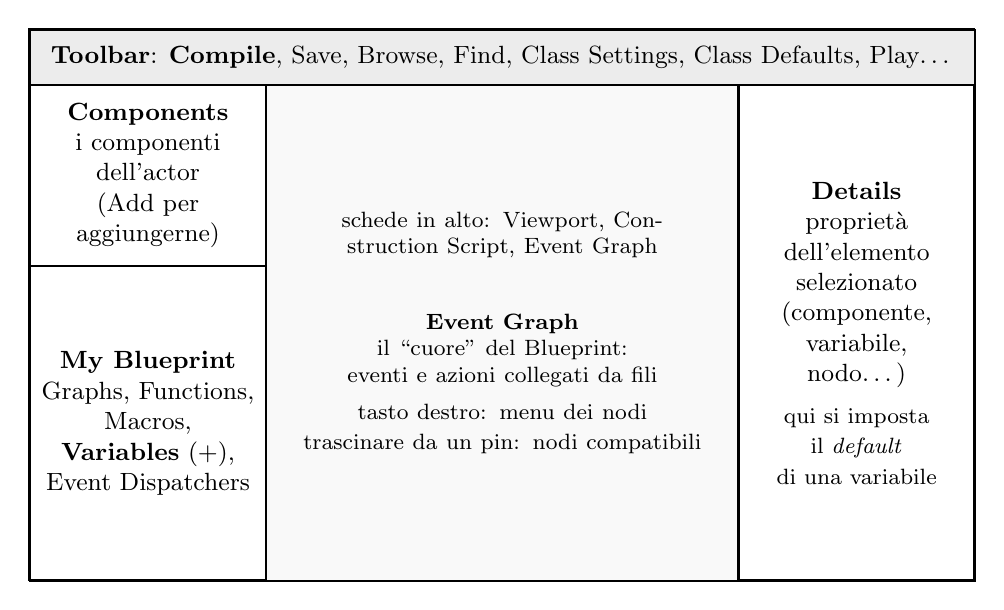
\begin{tikzpicture}[
  font=\small,
  ue2pan/.style={draw, thick, align=center, inner sep=3pt}
]
  \draw[thick] (0,0) rectangle (12,7);
  \node[ue2pan, minimum width=12cm, minimum height=0.7cm, anchor=north west,
    fill=gray!15] at (0,7) {\textbf{Toolbar}: \textbf{Compile}, Save, Browse, Find,
    Class Settings, Class Defaults, Play\ldots};
  \node[ue2pan, minimum width=3cm, minimum height=2.3cm, anchor=north west]
    at (0,6.3) {\textbf{Components}\\i componenti\\dell'actor\\(Add per\\aggiungerne)};
  \node[ue2pan, minimum width=3cm, minimum height=4cm, anchor=north west]
    at (0,4.0) {\textbf{My Blueprint}\\Graphs, Functions,\\Macros,\\
    \textbf{Variables} (+),\\Event Dispatchers};
  \node[ue2pan, minimum width=6cm, minimum height=6.3cm, anchor=north west,
    text width=5.6cm, fill=gray!5] at (3,6.3) {\footnotesize schede in alto:
    Viewport, Construction Script, Event Graph\\[18pt]\textbf{Event Graph}\\il ``cuore'' del Blueprint:\\
    eventi e azioni collegati da fili\\[4pt]\footnotesize tasto destro: menu dei nodi\\
    \footnotesize trascinare da un pin: nodi compatibili};
  \node[ue2pan, minimum width=3cm, minimum height=6.3cm, anchor=north west]
    at (9,6.3) {\textbf{Details}\\proprietà\\dell'elemento\\selezionato\\
    (componente,\\variabile,\\nodo\ldots)\\[4pt]\footnotesize qui si imposta\\
    \footnotesize il \emph{default}\\\footnotesize di una variabile};
\end{tikzpicture}
\caption{L'editor dei Blueprint (Blueprint Class Editor), ricostruito dalla lezione e
dal primo capitolo del libro di Romero e Sewell. La disposizione dei pannelli si può
cambiare, come nel Level Editor.}
\label{ue2:fig:editorbp}
\end{figure}

\paragraph{Approfondimento: i pannelli dell'editor.} Romero e Sewell, nel primo capitolo,
elencano i pannelli principali del \emph{Blueprint Class Editor}: la
\textbf{Toolbar}, i \textbf{Components} (i componenti già pronti che si aggiungono con
Add: \emph{mesh} statiche, luci, suoni, collisioni, particelle, camere), \textbf{My
Blueprint} (dove si creano variabili, macro, funzioni e grafi, con i pulsanti +), i
\textbf{Details} (le proprietà dell'elemento selezionato, con una barra di ricerca in
alto), la \textbf{Viewport} e l'\textbf{Event Graph}. Nell'Event Graph, notano gli
autori, un \textbf{evento} è un nodo \textbf{rosso}, e le altre azioni che seguono un
evento si collegano con dei fili; ci si sposta nel grafo trascinando con il tasto
destro. Di ogni evento se ne può mettere \textbf{uno solo} per grafo, ma si possono
creare eventi propri (\textbf{Add Custom Event}). Oltre a BeginPlay e Tick, il libro
cita gli eventi di \textbf{collisione} (quando due actor si scontrano o si
sovrappongono), gli eventi di \textbf{input} (tastiera, mouse, \emph{touch},
\emph{gamepad}) ed \textbf{Event End Play}, quando l'actor sta per essere rimosso.

% ---------------------------------------------------------------------
\section{Il primo nodo: Print String}
\label{ue2:sec:print}

``Andremo a fare una piccola prova.'' Unreal gestisce tutto con i \textbf{nodi}. Se si
porta il mouse sul ``pinnetto'' bianco a forma di freccia dell'Event BeginPlay, lo si
clicca e lo si \textbf{trascina verso l'esterno}, al rilascio compare un menu con tutti
i blocchi che si possono collegare: ``possiamo metterci tutto quello che vogliamo, tutti
i blocchi che ci serviranno per fare un'azione''.

\paragraph{Print String.} L'azione più semplice è \textbf{Print String}, che
``letteralmente ci stampa qualcosa a schermo''. Il testo predefinito è ``Hello''.

\paragraph{La barra ``Development Only''.} Igor fa notare un dettaglio. A differenza di
altri nodi, come \textbf{Set Actor Location} o \textbf{Enable Collision}, il Print String
ha una \textbf{barra in basso}. Vuol dire che quel blocco ha effetto \textbf{solo in
modalità di sviluppo}: quando si sviluppa e si va in Play nell'editor funziona, ma se si
facesse un \textbf{eseguibile} da mandare a qualcun altro ``questa cosa non avverrà
mai''. Gli altri nodi, invece, sì.

\paragraph{Compilare.} ``Molto importante'': quando si fanno dei cambiamenti
importanti bisogna \textbf{compilare} (\textbf{Compile}, in alto a sinistra). La
compilazione ``legge quello che abbiamo fatto'' e aggiorna il programma; in molti casi
Unreal lo fa anche in automatico, ma conviene farlo sempre. E \textbf{salvare},
``ovviamente, sempre buona cosa''.

\paragraph{La prova.} Si abbassa la finestra del Blueprint, si \textbf{mette l'actor
nella scena} (``ovviamente, se no non succede niente'': il Blueprint è solo una classe,
finché non se ne mette una copia nel livello non esiste) e si preme Play. In alto a
sinistra compare ``Hello'', ma per pochissimo. Igor cambia allora il parametro
\textbf{Duration} del nodo a 100 secondi, e la scritta resta: ``è piccolo'', ma c'è.
L'actor è entrato in funzione e ha fatto la sua azione appena ha cominciato a esistere,
cioè subito, perché era già nella scena.

\paragraph{Una finestra di gioco separata.} ``Se vi è più comodo'', si può far partire il
gioco in una finestra esterna: dai \textbf{tre puntini} accanto al pulsante Play si
sceglie \textbf{New Editor Window (PIE)}. ``Io lo trovo molto più comodo'': invece di
abbassare e rialzare la finestra del Blueprint, il gioco gira in una finestra a parte da
cui si controlla tutto. Igor lo scrive anche in chat.

\paragraph{Approfondimento: \emph{development} e \emph{shipping}.} La barra del Print
String rimanda a una distinzione che Romero e Sewell spiegano nel capitolo sul
\emph{packaging}: le \emph{build} di \textbf{sviluppo} (\emph{Development}) contengono
informazioni che servono al \emph{debug}, quelle di \textbf{distribuzione}
(\emph{Shipping}) sono più ``pulite'', senza informazioni di \emph{debug}, e sono quelle
da pubblicare. I nodi marcati \emph{Development Only}, come il Print String, vengono
semplicemente ignorati in una \emph{build} Shipping: si possono quindi lasciare nel
grafo mentre si lavora senza che il giocatore finale veda mai le scritte di prova.

% ---------------------------------------------------------------------
\section{Le variabili: GET e SET, colori e calcoli}
\label{ue2:sec:variabili}

\paragraph{Che cos'è una variabile.} Igor chiede chi abbia mai sentito parlare di
variabili \emph{bool}, \emph{float}, \emph{int}; qualcuno sì. Una \textbf{variabile} è
``uno slot di una tipologia di valore'' in cui si può mettere un valore: ``è come una
\textbf{scatola}''. Si creano delle piccole scatoline in cui mettere dei valori, ma ogni
scatola è fatta per un certo contenuto: ``c'è la scatola per i gioielli, c'è la scatola
per le praline'' (``mi invento un po' di cose''). Il tipo della variabile decide che cosa
ci si può mettere dentro.

\paragraph{Creare una variabile.} L'esempio: rendere ``esterna'' la durata del Print
String, cioè metterla in una variabile. Nel pannello My Blueprint, alla voce
\textbf{Variables}, si clicca \textbf{+}: si crea subito una variabile, di tipo booleano
oppure dello stesso tipo dell'ultima variabile creata. Igor la chiama \textbf{duration
time text}\footnote{Così nella trascrizione (una volta ``duration time next''); il nome
esatto digitato non si sente, ma non ha importanza per l'esempio.}.

\paragraph{GET e SET.} Se si trascina la variabile nel grafo, Unreal chiede se si vuole
un \textbf{GET} o un \textbf{SET}. GET è \textbf{prendere} il valore che c'è dentro; SET
è \textbf{impostare} il valore dentro. Per dare il valore alla durata del Print String
serve un GET.

\paragraph{I colori devono combaciare.} ``Però attenzione, che succede? Questo è rosso e
questo è verde.'' Il pin della variabile appena creata è \textbf{rosso} (è una
booleana), quello della Duration è \textbf{verde}: ``non sono della stessa tipologia''.
Due pin rossi si collegano; un rosso e un verde no. Il verde è il \textbf{float}. ``Cosa
sono i numeri float?'' ``I numeri con la virgola.'' ``Ottimo'': i numeri con i
\textbf{decimali}. Si cambia quindi il tipo della variabile in Float, il pin diventa
verde, e ``guardate un po', si collega''.

\paragraph{\emph{Please compile the Blueprint}.} Appena collegata, la variabile mostra
l'avviso \emph{please compile the blueprint}: è stata appena creata, e il Blueprint ``non
sa ancora che c'è una variabile nuova''. Dopo la compilazione, nei Details compare il
suo \textbf{valore predefinito} (\emph{Default Value}): ``guarda, questo è il tuo valore.
Quanto lo vuoi?'' Igor mette 10. In Play la scritta dura 10 secondi (``un po' tanti'') e
poi scompare: ``non è più 100''. La lezione: si possono creare variabili, impostarle e
darle ai blocchi di esecuzione.

\paragraph{Nodi di esecuzione e nodi di calcolo.} I \textbf{blocchi di esecuzione} si
riconoscono perché hanno l'intestazione \textbf{blu} e il pin di esecuzione, ``la
freccettina'' bianca. Ci sono però anche nodi \textbf{verdi} senza quel pin: sono nodi
che ``\textbf{calcolano solamente}''. Igor ne fa vedere uno, \textbf{Find Look at
Rotation}: chiede due variabili di un tipo e ne restituisce un'altra, dello stesso tipo
o di un altro. ``Oppure, esempio classico'': gli \textbf{operatori} aritmetici, il
\textbf{+}, il \textbf{$-$} (\emph{Subtraction}), il \textbf{per}, che si cerca con
l'\textbf{asterisco} (\emph{Multiply}), e il \textbf{diviso} (\emph{Divide}). Si
possono invocare tutti gli operatori che servono (figura~\ref{ue2:fig:pin}).

\paragraph{Sottrarre due secondi.} L'esempio: ``indipendentemente da quanto tempo noi
mettiamo qua dentro'', togliere sempre 2 secondi. Si prende il nodo meno, si collega la
variabile al primo ingresso (il nodo ``è diventato verde'', perché ha riconosciuto che si
tratta di un float, e ``ci chiede: te lo sottraggo di un altro float''), si scrive 2 nel
secondo e si collega il risultato alla Duration.

\paragraph{Da numero a testo.} Si può anche \textbf{stampare} il valore: collegando il
float all'ingresso di testo del Print String, Unreal inserisce in automatico un
\textbf{convertitore}. I pin \textbf{rosa} sono le \textbf{stringhe}, cioè testo. In
Play, il Print String non stampa più ``Hello'' ma \textbf{8}, ``che è 10 meno 2'', e la
scritta dura 8 secondi. (Ogni volta che Igor apre Unreal, Zoom va a scatti: ``a quanto
pare mi lagga Zoom benissimo''.)

\begin{figure}[htbp]
\centering
\begin{tikzpicture}[
  font=\small,
  ue2node/.style={draw, thick, rounded corners=4pt, align=center},
  ue2exec/.style={-{Stealth[length=2.5mm]}, very thick},
  ue2flt/.style={-{Stealth[length=2mm]}, thick, green!50!black},
  ue2str/.style={-{Stealth[length=2mm]}, thick, magenta}
]
  \node[ue2node, fill=red!15, minimum width=2.6cm, minimum height=1.2cm]
    (bp) at (0,0) {\textbf{Event}\\\textbf{BeginPlay}};
  \node[ue2node, fill=blue!10, minimum width=3.4cm, minimum height=2.6cm,
    anchor=north west] (pr) at (7.4,0.6) {};
  \node[font=\small\bfseries, anchor=north] at (pr.north) {Print String};
  \node[font=\footnotesize, anchor=west] (ins) at (7.5,-0.5) {In String};
  \node[font=\footnotesize, anchor=west] (dur) at (7.5,-1.2) {Duration};
  \node[font=\scriptsize\itshape, anchor=south] at (pr.south) {Development Only};
  \node[ue2node, fill=green!10, minimum height=0.8cm] (get) at (0.4,-1.9)
    {GET duration (float)};
  \node[ue2node, fill=green!10, minimum height=0.8cm] (minus) at (3.6,-1.9)
    {$x - 2$};
  \node[ue2node, fill=magenta!8, minimum height=0.8cm, font=\footnotesize]
    (conv) at (5.6,-0.5) {float $\to$ string};
  \draw[ue2exec] (bp.east) -- node[above, font=\footnotesize]{esecuzione}
    (bp.east -| pr.west);
  \draw[ue2flt] (get) -- (minus);
  \draw[ue2flt] (minus.east) -- ++(0.4,0) |- (dur.west);
  \draw[ue2flt] (minus.north) |- (conv.west);
  \draw[ue2str] (conv.east) -- (ins.west);
\end{tikzpicture}
\caption{Il primo grafo della lezione, nella sua versione finale: all'inizio del gioco
l'actor stampa la durata meno 2 (cioè 8) per 8 secondi. La freccia nera è il filo di
\textbf{esecuzione} (l'ordine delle azioni, da sinistra a destra); le frecce colorate
sono fili di \textbf{dati}, del colore del loro tipo (verde il float, rosa la stringa).
Il nodo blu, con il pin di esecuzione, è un'\textbf{azione}; i nodi verdi, senza, sono
nodi di \textbf{calcolo}, che si eseguono quando un'azione chiede il loro valore. Il
convertitore è inserito da Unreal in automatico. Schema ricostruito, non copia della
schermata.}
\label{ue2:fig:pin}
\end{figure}

% ---------------------------------------------------------------------
\section{Primo esercizio: Time To Print}
\label{ue2:sec:esercizio1}

``Vorrei fare un piccolo esercizio con voi. Molto velocissimo.''

\paragraph{Staccare un filo.} Prima, un comando: per \textbf{staccare} un collegamento
si tiene premuto \textbf{Alt} e si clicca sul pin.

\paragraph{La consegna.} Creare un'altra variabile, \textbf{time to print}, di tipo
\textbf{float}; staccare la variabile della durata dall'ingresso del testo e collegarci
invece time to print; dare a time to print il valore \textbf{5}, che dovrà essere
stampato a schermo. Anche la Duration va messa a 5. ``Senza che andiamo a vedere poi
ognuno'': l'importante è che ognuno dica ``stampa 5, sì''.

\paragraph{Un esercizio guidato.} Uno studente arriva in ritardo (``scusate, non
riuscivo ad entrare''). A una studentessa il Print String stampa \textbf{0}, e Igor la
guida passo per passo in condivisione dello schermo: fermare il gioco (lo
\textbf{Stop}, o il tasto \textbf{Esc}); creare la variabile dal \textbf{+} di Variables
nel pannello a sinistra; chiamarla time to print; cambiarle il tipo per farla
\textbf{verde}, cioè float (``bravissima''); prenderne il GET; staccare il vecchio
collegamento con Alt e attaccare time to print; compilare (``in alto a sinistra'');
poi, con la variabile selezionata, guardare nei \textbf{Details} a destra: ``vedi, adesso
è apparsa. In fondo''. In fondo ai Details c'è il \textbf{valore predefinito}, ed è lì
che si mette il 5. Lo 0 dipendeva proprio da questo: il valore predefinito di un float
appena creato è zero.

% ---------------------------------------------------------------------
\section{I dettagli di una variabile, e il \emph{tuning}}
\label{ue2:sec:dettagli}

Tutte le caratteristiche di una variabile si vedono nei \textbf{Details}, sia cliccando
la variabile nel grafo, sia cliccandola nella lista Variables. Igor consiglia di
impostare l'engine \textbf{in inglese} (``io sono più abituato all'inglese''), ma se si
trova più facile l'italiano non c'è nessun problema.

\paragraph{Il nome, il tipo, la descrizione.} Nei Details si possono cambiare il nome, il
tipo e una \textbf{descrizione}. La descrizione non la vedrà il giocatore, ma ``i nostri
amici programmatori, o comunque colleghi'': ci si può scrivere un piccolo commento,
come ``variabile da stampare nel Print''. È un'informazione ``per lo più organizzativa'',
``non un qualcosa che troverete spesso''.

\paragraph{Pubblica e privata: Instance Editable.} L'opzione \textbf{Instance Editable}
rende una variabile \textbf{pubblica}. Gli studenti non conoscono la distinzione ``in
questo contesto''. Una variabile \textbf{privata} esiste solo all'interno dell'actor;
una \textbf{pubblica} si può vedere e modificare direttamente nei \textbf{Details}
dell'actor piazzato nel livello. Uno studente chiede se sia come ``globale e locale''.
``Non esattamente, perché globale è anche un'altra cosa che andremo a vedere'': le
variabili davvero globali si fanno con la \textbf{Game Instance}, un oggetto che
\textbf{esiste finché esiste il gioco} e che può contenere variabili da ``dare in pasto''
a tutti gli actor che si vuole.

\paragraph{L'occhietto.} Lo stesso risultato si ottiene con l'icona
dell'\textbf{occhio} accanto alla variabile nella lista. Igor lo mostra: con l'occhio
aperto, selezionando l'actor nel livello, nei Details compare la sezione
\textbf{Default} con \emph{time to print}; con l'occhio chiuso, dopo aver ricompilato,
la voce scompare.

\paragraph{Il \emph{tuning}.} A che cosa serve? ``Il design è sempre con me.'' Come
designer, a Igor è capitato spesso di fare \textbf{\emph{tuning}}: la pratica di
\textbf{aggiustare i valori}, ``quanto danno fa, quanto fa di contrattacco'', in
generale i valori modificabili. Diceva al programmatore: ``lasciami quei valori, che li
devo controllare'', cioè testare. E poi andava nei Details dell'actor e cambiava
``questo, quell'altro, questo, quell'altro''. Le variabili pubbliche servono proprio a
questo: permettono di \textbf{interagire con l'editor stesso} senza toccare il grafo. Le
cose private, invece, restano nel campo dell'actor.

\paragraph{Approfondimento: gli attributi di una variabile.} Romero e Sewell, nel secondo
capitolo, elencano tutti gli attributi che i Details mostrano per una variabile.
\begin{itemize}
  \item \textbf{Variable Name} e \textbf{Variable Type}: il nome e il tipo. I Blueprint
        sono un linguaggio \textbf{fortemente tipizzato}: il tipo si sceglie alla
        creazione e non cambia durante l'esecuzione.
  \item \textbf{Instance Editable}: se attivo, \textbf{ogni copia} del Blueprint
        piazzata nel livello può avere un valore diverso; altrimenti tutte le copie
        (le \emph{istanze}) condividono lo stesso valore iniziale. È la precisazione
        tecnica del ``pubblico'' di Igor.
  \item \textbf{Blueprint Read Only}: se attivo, i nodi non possono modificare la
        variabile.
  \item \textbf{Tooltip}: il testo che compare passando il mouse sulla variabile; è la
        ``descrizione'' di cui parla Igor.
  \item \textbf{Expose on Spawn}: la variabile si può impostare nel momento in cui
        l'actor viene \emph{spawnato}.
  \item \textbf{Private}: se attivo, i Blueprint figli non possono modificarla.
  \item \textbf{Expose to Cinematics}: la rende visibile al Sequencer.
  \item \textbf{Category}: per raggruppare le variabili.
  \item \textbf{Slider Range} e \textbf{Value Range}: il minimo e il massimo, per lo
        \emph{slider} e per i valori ammessi. Per il \emph{tuning} sono preziosi: chi
        aggiusta i valori non può uscire dai limiti sensati.
  \item \textbf{Replication}: per i giochi in rete.
  \item \textbf{Default Value}: il valore iniziale; si può impostare solo dopo aver
        compilato, come si è visto nell'esercizio.
\end{itemize}

% ---------------------------------------------------------------------
\section{I tipi di variabile}
\label{ue2:sec:tipi}

Igor cancella tutto (seleziona e preme \textbf{Canc}, \emph{Delete} sulla tastiera
inglese) e passa a una slide sui tipi di variabile (tabella~\ref{ue2:tab:tipi}).
``Immaginiamoci sempre delle scatolette, con dentro dei valori.''

\paragraph{Booleana.} ``Qualcuno ha mai sentito parlare di booleane?'' Qualche sì,
qualche no. Una variabile \textbf{booleana} ha due valori possibili: \textbf{vero} o
\textbf{falso}. ``Dentro o c'è vero, o c'è falso, una delle due. Basta.'' Con un esempio
dall'elettrotecnica, è ``letteralmente lo \emph{switch} della luce'': spento è falso,
acceso è vero; a livello di circuito, ``è aperto o è chiuso''.

\paragraph{Byte, Integer, Integer64.} Il \textbf{byte} è un valore numerico intero
compreso tra 0 e 255. L'\textbf{integer}\footnote{Nella trascrizione ``gli integrali, i
numeri integrali''.}, o intero, è un numero \textbf{senza la virgola}: ``1, 2, 3, 4, 5,
6, 7, 8, senza virgola, senza niente'', compreso tra $-2^{31}$ e $2^{31}$ (``possiamo
anche non capire qual è il numero preciso, perché tanto è difficile che ci arriviamo'').
L'\textbf{integer64} arriva a 64 bit, tra $-2^{63}$ e $2^{63}$.

\paragraph{Float.} Il \textbf{float} è il valore numerico \textbf{con i decimali}.

\paragraph{Name, String, Text.} Il \textbf{name} è un testo usato principalmente per gli
\textbf{identificatori}, per identificare degli elementi in Unreal. La \textbf{string}
è un gruppo di caratteri \textbf{alfanumerici}, ``numeri e lettere''. Uno studente chiede
la differenza: anche il name è una stringa? La stringa, risponde Igor, si usa per lo più
nei \textbf{testi}; i name sono \textbf{nomenclature}: ``il nome di un livello, il nome
di un \emph{asset}''. ``Tipo un'etichetta'', propone lo studente: ``bravissimo, è come
un'etichetta'', ``quasi come un \textbf{tag}''. Il \textbf{text}, infine, è un testo
usato principalmente nella \textbf{UI}, la \emph{user interface}: tutto ciò che è 2D e
con cui l'utente interagisce, un termine usato ``in tanti campi, anche coi siti''.

\paragraph{Vector, Rotator, Transform.} I \textbf{vettori} sono ``molto importanti'',
essendo Unreal un ambiente tridimensionale. Un vettore può essere la
\textbf{locazione}: ``ci ricordiamo che quando abbiamo spostato i nostri cubetti e coni
abbiamo visto quei tre valori cambiare, la X, la Y e la Z?'' Un vettore è ``la
composizione'' di questi tre: una variabile che contiene \textbf{tre valori}, X, Y e Z.
Il \textbf{rotator} contiene gli X, Y e Z della \textbf{rotazione} (``poi faremo un po'
di discorsi, perché esistono i quaternioni, eccetera''). Il \textbf{transform}
contiene location, rotation e scala.

\paragraph{Object.} Infine il tipo \textbf{object}: ``volendo, noi potremmo creare una
variabile di tipologia di un actor che abbiamo creato''. È una variabile che contiene un
\textbf{riferimento} a un actor (si vedrà con il Level Blueprint,
sezione~\ref{ue2:sec:level}).

\begin{table}[htbp]
\centering
\small
\begin{tabular}{@{}p{2.2cm}p{2.0cm}p{8.8cm}@{}}
\toprule
\textbf{Tipo} & \textbf{Colore} & \textbf{Che cosa contiene} \\
\midrule
Boolean & rosso & vero o falso (\emph{true}/\emph{false}) \\
Byte & verde scuro & intero da 0 a 255 (8 bit) \\
Integer & verde acqua & intero da $-2^{31}$ a $2^{31}-1$ (32 bit) \\
Integer64 & verde acqua scuro & intero da $-2^{63}$ a $2^{63}-1$ (64 bit) \\
Float & verde & numero con decimali; in Unreal Engine 5 i Blueprint lo trattano in
  precisione singola o doppia (\emph{Double}) \\
Name & lilla & identificatore, ``etichetta'' (nome di un livello, di un \emph{asset}) \\
String & rosa & gruppo di caratteri alfanumerici \\
Text & rosa scuro & testo per la UI, \textbf{localizzabile} (traducibile) \\
Vector & giallo & tre float X, Y, Z (per esempio una locazione) \\
Rotator & viola-lilla & tre float della rotazione: X (\emph{roll}), Y (\emph{pitch}),
  Z (\emph{yaw}) \\
Transform & arancione & locazione, rotazione e scala \\
Object & blu & riferimento a un oggetto (per esempio un actor nel livello) \\
\bottomrule
\end{tabular}
\caption{I tipi di variabile della slide di Igor, con i colori dei loro pin
nell'editor (i nomi dei colori sono approssimativi) e le integrazioni del libro di
Romero e Sewell (i limiti esatti degli interi, \emph{roll}, \emph{pitch} e \emph{yaw},
la localizzazione del Text).}
\label{ue2:tab:tipi}
\end{table}

\paragraph{Approfondimento: Double, Text e i tre angoli.} Tre precisazioni dal secondo
capitolo del libro. Primo: oltre al Float a 32 bit (sette cifre decimali di
precisione) esiste il \textbf{Double} a 64 bit (sedici cifre); in Unreal Engine 5 l'editor
mostra entrambi come ``Float'' e sceglie la precisione da solo. Secondo: il
\textbf{Text} serve ai testi che saranno \textbf{localizzati}, cioè tradotti in altre
lingue: è per questo che è il tipo della UI, mentre String è il testo ``di servizio'' e
Name l'identificatore. Terzo: i tre valori del \textbf{Rotator} hanno un nome. X è il
\textbf{\emph{roll}} (il rollio, la rotazione attorno all'asse X, quello ``in avanti''),
Y il \textbf{\emph{pitch}} (il beccheggio, attorno all'asse Y, alzare o abbassare il
muso), Z lo \textbf{\emph{yaw}} (l'imbardata, attorno all'asse Z verticale, girare a
destra e a sinistra). Sono i nomi che compariranno nei nodi della piattaforma
(sezione~\ref{ue2:sec:mouse}). I \textbf{quaternioni} a cui accenna Igor sono un altro
modo, matematicamente più robusto, di rappresentare una rotazione: evitano il problema
del \emph{gimbal lock}, in cui due dei tre assi finiscono per coincidere e si perde un
grado di libertà. Unreal li usa al suo interno, ma nei Blueprint si lavora quasi sempre
con i Rotator.

% ---------------------------------------------------------------------
\section{Le booleane e il Branch}
\label{ue2:sec:branch}

``Adesso vi faccio vedere.'' Igor crea una variabile, la chiama ``letteralmente''
\textbf{bool}, e le dà il tipo booleano.

\paragraph{GET e SET in un gesto.} ``Piccola cosetta'': invece di scegliere dal menu, si
può fare un GET ``velocissimamente'' trascinando la variabile nel grafo con
\textbf{Ctrl} premuto, e un SET trascinandola con \textbf{Alt}. Il \textbf{GET} è il pin
che dice ``questa è la scatoletta che c'è dentro qualcosa, prendi il valore da qui''. Il
\textbf{SET} è diverso: ha un \textbf{nodo di esecuzione}, a differenza del GET, e ha una
\textbf{casella di spunta}\footnote{Nella trascrizione ``un TIL'': è il \emph{tick},
la spunta della casella.}: cliccandola si imposta il valore. ``Col SET sto letteralmente
impostando il suo valore'': spunta, vero; niente spunta, falso.

\paragraph{Stampare una booleana.} Igor rifà un Print String con Duration 10 (``sennò è
troppo poco''), collega il pin della booleana al testo e va in Play: in alto a sinistra
compare \textbf{false}. Mette la spunta, rifà Play: \textbf{true}. Il Print String
riceve, tramite la stringa, il valore della variabile.

\paragraph{A che cosa serve sapere se è vero o falso?} ``La domanda magari è: ok, ma che ci
serve?'' Serve perché si possono usare delle \textbf{condizioni}. ``Qualcuno ha mai
sentito parlare di \emph{if}, \emph{else}?'' Edoardo sì: ``ho studiato informatica alle
superiori''. ``Grande, perfetto.'' L'\textbf{if-else} è una condizione, e in Unreal non si
chiama così: tenendo premuto \textbf{B} e cliccando nel grafo compare il
\textbf{Branch}, ``cioè due percorsi''. È ``un \textbf{bivio}'': ``se questa condizione
che abbiamo qua è vera, vai per questo percorso; se questa condizione è falsa, vammi per
un altro''.

\paragraph{Il primo Branch.} Igor collega il Branch dopo il BeginPlay e porta la
variabile bool nel pin rosso \textbf{Condition}. Sull'uscita \textbf{True} mette un Print
String con ``la variabile è vera''; per l'uscita \textbf{False} copia il nodo (``per
copiare qualcosa, Ctrl+C, Ctrl+V, classico'') e scrive ``la variabile è falsa''. Con la
variabile falsa, in Play esce ``la variabile è falsa''; con la spunta, ``la variabile è
vera'' (figura~\ref{ue2:fig:branch}).

\paragraph{I binari del treno.} ``Letteralmente sta prendendo un bivio: o vado di qua, o
vado di là.'' Igor lo paragona ai \textbf{binari di un treno}: ``se la leva è a destra,
vado a destra; se la leva è a sinistra, vado a sinistra. E la nostra leva è la nostra
variabile''. Il bool è molto importante perché permette di avere delle condizioni, e
quindi gli attori ``\textbf{pensano}'': hanno la ``capacità di scelte'', ``ah, ok, allora
prendo questa strada perché ho questa variabile di questo tipo''.

\begin{figure}[htbp]
\centering
\begin{tikzpicture}[
  font=\small,
  ue2node/.style={draw, thick, rounded corners=4pt, align=center,
                  minimum height=1cm},
  ue2exec/.style={-{Stealth[length=2.5mm]}, very thick},
  ue2bool/.style={-{Stealth[length=2mm]}, thick, red!70!black}
]
  \node[ue2node, fill=red!15, minimum width=2.4cm] (bp) at (0,0)
    {\textbf{Event}\\\textbf{BeginPlay}};
  \node[ue2node, fill=gray!10, minimum width=2.2cm, minimum height=1.6cm]
    (br) at (4,0) {\textbf{Branch}\\[2pt]\footnotesize Condition};
  \node[ue2node, fill=green!8, minimum width=1.6cm] (get) at (1.6,-1.8) {GET bool};
  \node[ue2node, fill=blue!10, text width=3.6cm] (pt) at (9,0.9)
    {\textbf{Print String}\\\footnotesize ``la variabile è vera''};
  \node[ue2node, fill=blue!10, text width=3.6cm] (pf) at (9,-0.9)
    {\textbf{Print String}\\\footnotesize ``la variabile è falsa''};
  \draw[ue2exec] (bp) -- (br);
  \draw[ue2bool] (get.east) -| ([xshift=-4mm]br.south);
  \draw[ue2exec] ([yshift=4mm]br.east) -- node[above, font=\footnotesize]{True}
    ++(1.2,0) |- (pt.west);
  \draw[ue2exec] ([yshift=-4mm]br.east) -- node[below, font=\footnotesize]{False}
    ++(1.2,0) |- (pf.west);
\end{tikzpicture}
\caption{Il Branch è un bivio: segue l'uscita True o l'uscita False a seconda del valore
della condizione. ``La nostra leva è la nostra variabile.''}
\label{ue2:fig:branch}
\end{figure}

\paragraph{Si può accedere al codice?} Uno studente chiede se sia possibile accedere anche
al codice, ``immagino che sia C''. Sì, è possibile, ``però non lo faremo''. Con il C++ si
possono definire anche i blocchi stessi, creare blocchi di tipo diverso; ma ``di base, su
Blueprint possiamo farlo allo stesso modo anche noi''. Chi vuole può andare a vederlo; e
c'è chi va ``proprio nel profondo della programmazione'', come gli \emph{engine
programmer}.

\paragraph{Allineare i nodi.} ``Una piccola cosa, se vi piace l'ordine'': si selezionano
due nodi e si preme \textbf{Q}, e Unreal li allinea.

\paragraph{Approfondimento: Branch e operatori relazionali.} Romero e Sewell presentano il
Branch nel secondo capitolo, parlando del \textbf{percorso di esecuzione}: i pin bianchi
sono i \textbf{pin di esecuzione}, gli altri, colorati, i \textbf{pin di dati};
l'esecuzione parte da un evento rosso e segue il filo bianco da sinistra a destra fino
all'ultimo nodo. Alcuni nodi, come il Branch, \textbf{controllano il flusso}: decidono
quale strada prendere. Il loro esempio è un personaggio con una booleana \emph{Has
Shield}: se è vera, il Branch imposta \emph{Shield Value} a 100; se è falsa, a 0. Nella
lezione la condizione è sempre una variabile booleana; nella pratica, spesso, è il
risultato di un \textbf{operatore relazionale}: i nodi $<$, $\leq$, $>$, $\geq$, $=$,
$\neq$ confrontano due valori e restituiscono una booleana. L'esempio del libro: quando
un oggetto subisce danni, un Branch controlla se \emph{Health} $\leq 0$, e in quel caso
l'oggetto viene distrutto; se no, non succede niente, perché all'uscita False non è
collegato nulla. Quanto alla scorciatoia: nel menu che si apre con il tasto destro su
una selezione di nodi c'è la voce \textbf{Alignment}, con allineamenti in alto, al
centro, in basso, a sinistra, a destra, e \textbf{Straighten Connection(s)}, che
raddrizza i fili; il tasto \textbf{Q} è la scorciatoia di quest'ultima. Il libro ricorda
anche le altre scorciatoie ``tasto + clic'': \textbf{B} per il Branch, \textbf{S} per il
nodo Sequence, \textbf{D} per il Delay, \textbf{F} per il For Each Loop
(tabella~\ref{ue2:tab:scorciatoie}).

% ---------------------------------------------------------------------
\section{Gli operatori logici: AND, OR, NOT}
\label{ue2:sec:logici}

Igor cancella i nodi di prova (``tanto non ci sono problemi'') e passa agli
\textbf{operatori logici}. ``Qualcuno ha mai sentito parlare di AND, OR, NOT?'' Sì.

\paragraph{Il gioco dei tubi.} A che cosa servono? Una variabile booleana ha i suoi valori,
vero e falso; ``però mettiamo conto che ne abbiamo altre'', e bisogna metterle in
\textbf{comparazione}. L'esempio è ``il gioco dei tubi'', l'enigma in cui bisogna girare i
tubi nel verso giusto per collegarli. Se ci sono due tubi, per risolvere l'enigma un tubo
deve essere girato nel modo giusto \textbf{e} anche l'altro: sono \textbf{due
condizioni} da prendere insieme. ``Come facciamo a metterle insieme?''

\paragraph{I nodi.} Igor crea una seconda booleana, \textbf{bool 2}. Gli operatori si
cercano scrivendo \textbf{OR Boolean}, \textbf{AND Boolean} e \textbf{NOT Boolean}.
``Questi sono i tre più usati''; ce ne sono altri, come il NOR, ``ma sono un attimo da
vedere poi più avanti''.

\paragraph{OR.} L'OR dice: ``se almeno un valore è vero, allora la condizione finale è
vera''. Con bool vera e bool 2 falsa, collegato alla condizione del Branch, esce ``la
variabile è vera''. È ``un modo per sommare le variabili tra \emph{true} e \emph{false}'',
``una specie di somma, chiamiamola così'': ``letteralmente dice: o questa, o questa''.

\paragraph{AND.} L'AND, con gli stessi valori, vero e falso, dà ``la variabile è falsa'',
``perché AND vuol dire \emph{questa e questa}'': tutte le condizioni devono essere vere
perché il risultato sia vero. Igor mette vera anche la seconda e\ldots{} non succede
niente: ``scusate, questo non l'ho collegato, sono io''. Collegato, esce ``la variabile è
vera''. Ricapitolando: se tutte e due sono vere, è vero; se una sola è falsa, ``tutto
quanto è falso''; se tutte e due sono false, è falso (``doppio falso'').

\paragraph{NOT.} Il NOT ha un solo ingresso e ``letteralmente \textbf{inverte}'': se la
variabile è vera diventa falsa, se è falsa diventa vera. Collegato a una variabile vera,
dà falso. ``Non lo useremo tanto.'' La tabella~\ref{ue2:tab:logici} riassume i tre
operatori.

\begin{table}[htbp]
\centering
\small
\begin{tabular}{@{}cc|ccc|ccc@{}}
\toprule
\textbf{A} & \textbf{B} & \textbf{A OR B} & \textbf{A AND B} & \textbf{NOT A} &
  \textbf{A NOR B} & \textbf{A NAND B} & \textbf{A XOR B} \\
\midrule
falso & falso & falso & falso & vero  & vero  & vero  & falso \\
falso & vero  & vero  & falso & vero  & falso & vero  & vero  \\
vero  & falso & vero  & falso & falso & falso & vero  & vero  \\
vero  & vero  & vero  & vero  & falso & falso & falso & falso \\
\bottomrule
\end{tabular}
\caption{Le tabelle di verità degli operatori logici. Le prime tre colonne di risultati
sono gli operatori della lezione; le ultime tre sono un'integrazione dal libro di Romero
e Sewell.}
\label{ue2:tab:logici}
\end{table}

\paragraph{Approfondimento: NOR, NAND, XOR, e perché l'OR è una ``somma''.} Il libro
completa la lista degli operatori logici dei Blueprint con tre combinazioni. Il
\textbf{NOR} (NOT + OR) è vero solo se entrambi gli ingressi sono falsi; il \textbf{NAND}
(NOT + AND) è falso solo se entrambi sono veri; lo \textbf{XOR}, l'OR esclusivo, è vero
se i due ingressi sono \textbf{diversi}. L'esempio del libro per l'AND: un Print String
che si esegue solo se \emph{Health} $> 70$ \textbf{e} \emph{Shield Value} $> 50$, con
due operatori relazionali che alimentano un AND. Quanto alla ``somma'' di Igor, è
un'intuizione che ha un nome: nell'\textbf{algebra di Boole}, da cui il tipo
\emph{boolean} prende il nome, l'OR si scrive come una somma ($A + B$) e l'AND come un
prodotto ($A \cdot B$). Se si leggono vero e falso come 1 e 0, l'AND si comporta
esattamente come una moltiplicazione (basta uno 0 per fare 0), e l'OR come una somma
in cui ``1 + 1'' resta 1.

% ---------------------------------------------------------------------
\section{Secondo esercizio: due Branch, OR e AND}
\label{ue2:sec:esercizio2}

``Allora facciamo un piccolo esercizio.''

\paragraph{La consegna.} All'Event BeginPlay si collega un \textbf{SET} della variabile
bool (quello che si ottiene trascinandola con Alt), e il suo valore va alla condizione
di un \textbf{primo Branch}. Su ciascuna uscita del primo Branch va un \textbf{secondo
Branch}: su True un Branch la cui condizione è \textbf{bool OR bool 2}; su False un
Branch la cui condizione è \textbf{bool AND bool 2}. Solo se il secondo Branch è vero si
stampa, e invece di ``la variabile è vera'' si stampa \textbf{il valore finale} del
calcolo, collegando l'uscita dell'operatore all'In String
(figura~\ref{ue2:fig:esercizio2}). ``Ce la fate?'' Cinque minuti.

\begin{figure}[htbp]
\centering
\begin{tikzpicture}[
  font=\small,
  ue2node/.style={draw, thick, rounded corners=4pt, align=center,
                  minimum height=0.9cm},
  ue2exec/.style={-{Stealth[length=2.5mm]}, very thick},
  ue2bool/.style={-{Stealth[length=2mm]}, thick, red!70!black}
]
  \node[ue2node, fill=red!15] (bp) at (0,0) {\textbf{BeginPlay}};
  \node[ue2node, fill=blue!10] (set) at (2.6,0) {\textbf{SET bool}\\\footnotesize
    $\square$ / $\checkmark$};
  \node[ue2node, fill=gray!10] (b1) at (5.2,0) {\textbf{Branch 1}\\\footnotesize
    cond.\ = bool};
  \node[ue2node, fill=gray!10] (b2) at (8.4,1.5) {\textbf{Branch 2}};
  \node[ue2node, fill=gray!10] (b3) at (8.4,-1.5) {\textbf{Branch 3}};
  \node[ue2node, fill=green!8] (or) at (8.4,3.1) {bool \textbf{OR} bool 2};
  \node[ue2node, fill=green!8] (and) at (8.4,-3.1) {bool \textbf{AND} bool 2};
  \node[ue2node, fill=blue!10, text width=2.3cm] (p1) at (11.6,1.5)
    {\textbf{Print}\\\footnotesize risultato OR};
  \node[ue2node, fill=blue!10, text width=2.3cm] (p2) at (11.6,-1.5)
    {\textbf{Print}\\\footnotesize risultato AND};
  \draw[ue2exec] (bp) -- (set);
  \draw[ue2exec] (set) -- (b1);
  \draw[ue2exec] (b1.east) ++(0,0.2) -- ++(0.5,0) |- node[pos=0.75, above,
    font=\footnotesize]{True} (b2.west);
  \draw[ue2exec] (b1.east) ++(0,-0.2) -- ++(0.5,0) |- node[pos=0.75, below,
    font=\footnotesize]{False} (b3.west);
  \draw[ue2bool] (or) -- (b2);
  \draw[ue2bool] (and) -- (b3);
  \draw[ue2exec] (b2) -- node[above, font=\footnotesize]{True} (p1);
  \draw[ue2exec] (b3) -- node[below, font=\footnotesize]{True} (p2);
  \draw[ue2bool, dashed] (or.east) -| (p1.north);
  \draw[ue2bool, dashed] (and.east) -| (p2.south);
\end{tikzpicture}
\caption{Il secondo esercizio. Le frecce nere sono l'esecuzione, quelle rosse i valori
booleani (tratteggiate: il risultato dell'operatore, convertito in testo e stampato). Le
uscite False dei Branch 2 e 3 non sono collegate: in quei casi non si stampa niente.}
\label{ue2:fig:esercizio2}
\end{figure}

\paragraph{Le domande durante l'esercizio.} Lo studente arrivato in ritardo chiede come
si crea il Print String: tasto destro, Print String. Un altro si è perso gli operatori:
si scrivono proprio ``AND Boolean'', ``OR Boolean'', ``NOT Boolean''. Una studentessa non
ricorda come si prende ``l'oggetto con il pallino rosso'' (la variabile): ``mettilo qua
dentro, ti appare in automatico''. Trascinando la variabile direttamente sul pin, Unreal
crea da solo il GET.

\paragraph{La spunta che non c'entra.} Un'altra studentessa ha un problema: sul primo
Branch, nella condizione, ha una \textbf{spunta} che Igor non ha. Il pin Condition non è
collegato all'\textbf{uscita} del SET. ``Devi collegare questo pallino a questo
pallino.'' Igor spiega che cosa è successo, con una dimostrazione. Il nodo SET ha a
destra un pin di uscita: ``è il valore che io gli ho impostato'', che esce dal nodo
``come un collegamento''. Il Branch ha a sinistra ``un posto in cui posso mettere quel
valore''. Se il pin non è collegato, la casella di spunta del Branch è una
\textbf{condizione interna al Branch}, che non ha niente a che vedere con la variabile:
``la porta si aprirà secondo bool, non secondo questa condizione qua''. Igor mette la
variabile a vero e la spunta del Branch a falso: il Print String collegato al True
``non mi stampa niente'', ``perché questa qua non è relativa a questa''. Collegando il
pin, stampa. (``Stavo impazzendo perché non mi stampava niente.'')

\paragraph{I ``what if''.} Poi Igor cerca ``un candidato'' per una piccola verifica:
``se io adesso vi cambio un po' i parametri, dove andiamo a finire con tutte le linee?''
Si offre uno studente.
\begin{itemize}
  \item \textbf{bool vero, bool 2 falso.} ``Siccome è \emph{true}, finisce sopra, sul
        primo Branch'' (il Branch 2 della figura). ``Controlla se tra bool e bool 2 uno
        dei due è vero. In questo caso lo è, perché hai settato bool come vero. Il
        secondo non è importante.'' Quindi va su True e stampa il valore. ``Perfetto.
        Netto, liscio.''
  \item \textbf{bool falso.} ``False scende giù e controlla se entrambi, bool e bool 2,
        sono veri. In questo caso bool è falso, quindi anche qui il secondo valore non
        è importante, perché uno dei due è falso. Il risultato dell'AND è falso e non
        stampa niente.'' ``Esatto, perfetto.''
\end{itemize}
La morale: ``indipendentemente dalle condizioni, possiamo cambiare i binari di un
percorso di programmazione''. È ``una delle cose più principali'', e serve molto spesso
per \textbf{diversificare i comportamenti} dei Blueprint. Igor chiede ancora se ci sono
domande, e decide di non cancellare il grafo ma di lasciarlo lì, scollegato. ``Sono stato
chiaro, dai.''

\paragraph{Approfondimento: la valutazione ``pigra''.} Lo studente coglie, senza
nominarlo, un principio importante: in un OR, se il primo ingresso è vero il secondo
``non è importante''; in un AND, se il primo è falso il secondo non cambia il risultato.
In molti linguaggi di programmazione questo si chiama \emph{short-circuit evaluation}
(valutazione a corto circuito): il secondo operando non viene nemmeno calcolato. Nei
nodi Blueprint, attenzione, i due ingressi vengono comunque calcolati entrambi; ma il
ragionamento sul \emph{risultato} è lo stesso, ed è quello che serve per prevedere dove
andrà l'esecuzione.

% ---------------------------------------------------------------------
\section{Il Level Blueprint e la piattaforma}
\label{ue2:sec:level}

``Adesso andremo a fare una piccola cosa direttamente nel nostro bellissimo Blueprint.''
L'obiettivo è una \textbf{piattaforma} che \textbf{ruota}, cioè si inclina, ``a seconda
di quanto premiamo'' dei tasti (D, A, e così via).

\paragraph{La piattaforma.} Si prende un \textbf{cubo} dal pannello Place Actors, lo si
mette in scena e lo si allarga ``quanto volete'', fino a farne una piattaforma.

\paragraph{Il Level Blueprint.} ``Vi farò conoscere il bellissimo mondo del \textbf{Level
Blueprint}.'' In Unreal esiste anche un Blueprint \textbf{interno al livello}: quando si
apre quel livello, al suo interno ci sono delle regole (``spawna qualcosa'', eccetera).
Lo si apre dall'icona dei Blueprint nella barra in alto: \textbf{Open Level Blueprint}.
Una studentessa si è persa (``scusa, come lo apriamo?''), e Igor le mostra l'icona.

\paragraph{Un evento di input.} Si è parlato di eventi con le loro condizioni; uno dei più
semplici è l'\textbf{input}. Tasto destro nel grafo, si scrive \textbf{W} e si sceglie
la voce con ``l'immaginetta della tastierina'' e la W: è un evento che scatta
\textbf{alla pressione del tasto W}.

\paragraph{La referenza.} Ma come si dice al grafo che deve agire su \emph{quella}
piattaforma? Si crea una \textbf{referenza}. Con il cubo selezionato nel livello, nel
Level Blueprint si fa tasto destro e si sceglie \textbf{Create a Reference to Cube94}
(il cubo di Igor si chiama Cube94, e lo si ritrova con quel nome nell'Outliner). ``Questo
può essere fatto solo nel Level Blueprint, ve lo dico.''

\paragraph{Set Actor Rotation e i suoi pin.} Dalla referenza si trascina un filo e si
sceglie \textbf{Set Actor Rotation}. Il nodo ha tre pin di dati:
\begin{itemize}
  \item un pin \textbf{blu}, il \textbf{Target}: un \emph{Actor Object Reference}, cioè
        una variabile che si riferisce a un actor, a uno qualunque degli elementi della
        \emph{viewport}, ``che abbiano programmazione o meno''. È l'actor su cui il nodo
        agisce;
  \item un pin \textbf{lilla}, \textbf{New Rotation}: un \textbf{rotator}, la
        composizione degli assi X, Y e Z della rotazione;
  \item un pin \textbf{rosso}, un \textbf{bool}: \textbf{Teleport} (tornerà utile con
        la fisica, sezione~\ref{ue2:sec:fisica}).
\end{itemize}

\paragraph{Il Player Start.} Per vedere la piattaforma serve un punto da cui partire.
``Prendete il \textbf{Player Start}'': lo si trova nel Place Actors, o cercandolo, ed è
``un controllone'' (l'icona di un \emph{joystick}). Lo si mette davanti alla piattaforma
e lo si gira verso di essa.

\paragraph{Consume Input.} Selezionando l'evento W, nei Details c'è una casella
interessante, \textbf{Consume Input}. Se è spuntata, il tasto W ``sarà dedicato solo a
questo evento'': il giocatore non potrà più usarlo per muoversi in avanti. Senza la spunta
si muoverebbe ``avanti e indietro''; ``a noi interessa stare fermi'', quindi la spunta
resta.

\paragraph{Quale asse, e in che verso.} La piattaforma va ruotata attorno all'asse
\textbf{X}. In positivo o in negativo? Igor lo verifica nella \emph{viewport} ruotando il
cubo: in un verso la rotazione è negativa, nell'altro positiva. ``Per come mi regolo'',
W manda la piattaforma in avanti, quindi si piega in un verso, e indietro nell'altro.
Igor scrive 5 nella X del New Rotation e prova.

% ---------------------------------------------------------------------
\section{La mobilità: Static, Stationary, Movable}
\label{ue2:sec:mobilita}

Non funziona, ``giustamente'', e Unreal mostra un avviso: ``ricordate che questo che mi è
appena uscito è un problema che Unreal ci darà sempre''. L'actor non ha la capacità di
essere \textbf{Movable}: non si può muovere nel mondo.

\paragraph{Dove si trova.} Nel \emph{transform} dell'actor, sotto location, rotation e
scala, c'è la \textbf{Mobility}, con tre valori: \textbf{Static}, \textbf{Stationary} e
\textbf{Movable}. È ``la tipologia di oggetto'' rispetto a come reagisce al mondo, e
riguarda ``soprattutto il rendering''.
\begin{itemize}
  \item \textbf{Static.} L'oggetto sa che non si muoverà. Quando si calcolano le luci,
        la sua ombra viene calcolata una volta e poi è come \textbf{dipinta}: ``è
        dipinta''. ``Per alleggerirsi la cosa'', l'engine dice: è un oggetto statico,
        ``basta che mi calcolo una volta l'ombra e basta''.
  \item \textbf{Stationary.} Una via di mezzo: le ombre vengono messe in
        \emph{cache}\footnote{Nella trascrizione ``vengono chesciate'': con ogni
        probabilità ``cachate'', dall'inglese \emph{cached}.}, l'oggetto può essere
        cambiato, ma non può essere mosso.
  \item \textbf{Movable.} Totalmente \textbf{dinamico}.
\end{itemize}
La piattaforma va messa su \textbf{Movable}, e allora ruota di 5 gradi. Igor prova con
valori più grandi (``facciamo tipo 25'') per vederlo meglio.

\paragraph{Approfondimento: la mobilità secondo il libro.} Romero e Sewell incontrano lo
stesso problema nel quinto capitolo, quando un bersaglio cilindrico deve cominciare a
muoversi: bisogna prima portare la sua Mobility da Static a \textbf{Movable}, nei Details
sotto il TRANSFORM. E aggiungono una nota importante: gli actor di base piazzati nel
mondo sono \textbf{Static per impostazione predefinita}, e gli oggetti statici sono
``significativamente meno costosi'' da renderizzare; per questo Static dovrebbe essere
la scelta predefinita per tutto ciò che non è interattivo, per tenere alto il
\emph{frame rate}. Stationary ha senso soprattutto per le \textbf{luci}: una luce
Stationary non si sposta, ma se ne possono cambiare colore e intensità durante il gioco,
e parte della sua illuminazione è precalcolata. Movable va riservato agli oggetti che
devono davvero muoversi.

% ---------------------------------------------------------------------
\section{Ruotare di 5 gradi a ogni pressione: Split Struct Pin}
\label{ue2:sec:split}

\paragraph{Funziona una volta sola.} ``Però che succede? Guardate un po'.'' Se si preme
di nuovo W, la piattaforma non fa niente. Il problema è che la si sta impostando a un
\textbf{valore preciso}: Set Actor Rotation dice ``mettiti a 25 gradi'', e la seconda
volta la piattaforma risponde ``ci sto già, a 25''. Serve invece una rotazione che
\textbf{parta da quella attuale}.

\paragraph{Prendere i valori dell'actor.} Igor mostra che dalla referenza di un actor si
possono prendere \textbf{tutti} i suoi valori: la location, la rotation, la scala, la
\emph{mesh}, i materiali (``che poi vedremo''). ``È andare nella scatola di
quell'\emph{asset}'': prendo quel valore, e poi lo modifico. Qui serve \textbf{Get Actor
Rotation}, la rotazione attuale, ``che si aggiorna ogni volta''.

\paragraph{Split Struct Pin.} La rotazione è data da tre valori, X, Y e Z, e se ne vuole
modificare uno solo. Con il tasto destro sul pin del Rotator si sceglie \textbf{Split
Struct Pin}: il pin si divide nei suoi tre valori, ``e guardate un po', la cosa bella è
che sono cambiati di colore''. Sono diventati \textbf{verdi}, ``perché sono tre valori
float''. Uno studente chiede come si fa a trovare i tre valori; Igor rifà il gesto
all'indietro (\textbf{Recombine Struct Pin}) e poi di nuovo avanti: tasto destro, Split
Struct Pin. Si fa lo stesso sul pin New Rotation del Set Actor Rotation, che altrimenti,
lilla, non accetterebbe un float.

\paragraph{Il grafo.} Si prende la X di Get Actor Rotation, le si somma 5 con un nodo
\textbf{+}, e il risultato va nella X del Set Actor Rotation
(figura~\ref{ue2:fig:piattaforma}, a sinistra). Ora la piattaforma si inclina di 5 gradi
a ogni pressione di W: ``posso aggiungere quanto me ne pare'', a parte che a un certo
punto la piattaforma \textbf{compenetra} il pavimento. ``Prima non andava bene e adesso
invece sì'', perché ogni volta si parte dalla rotazione attuale. Con un Print String
collegato alla X, a ogni pressione compaiono i valori \textbf{0, 5, 10, 15, 20, 25, 30,
35}: ``si aumenta sempre''.

\begin{figure}[htbp]
\centering
\begin{tikzpicture}[
  font=\small,
  ue2node/.style={draw, thick, rounded corners=4pt, align=center,
                  minimum height=0.9cm},
  ue2exec/.style={-{Stealth[length=2.5mm]}, very thick},
  ue2flt/.style={-{Stealth[length=2mm]}, thick, green!50!black},
  ue2obj/.style={-{Stealth[length=2mm]}, thick, blue!70!black}
]
  % versione prima della pausa
  \node[font=\footnotesize\bfseries] at (2.6,2.2) {Prima della pausa};
  \node[ue2node, fill=red!15] (w) at (0,1.2) {\textbf{W}\\\footnotesize Pressed};
  \node[ue2node, fill=blue!10, text width=3.2cm] (set) at (4.6,1.2)
    {\textbf{Set Actor Rotation}\\\footnotesize New Rotation (split)};
  \node[ue2node, fill=blue!5] (ref) at (0,-0.6) {Cube94};
  \node[ue2node, fill=green!8, text width=2.0cm] (get) at (2.0,-1.9)
    {\textbf{Get Actor Rotation}\\\footnotesize (split)};
  \node[ue2node, fill=green!8] (plus) at (4.6,-0.6) {X $+\,5$};
  \draw[ue2exec] (w) -- (set);
  \draw[ue2obj] (ref.east) -- ++(0.4,0) |- (get.west);
  \draw[ue2obj] (ref.north) -- ++(0,0.3) -| ([xshift=-12mm]set.south);
  \draw[ue2flt] (get.east) -| (plus.south);
  \draw[ue2flt] (plus) -- (set);
  % separatore
  \draw[gray, dashed] (7.2,2.4) -- (7.2,-2.6);
  % versione dopo la pausa
  \node[font=\footnotesize\bfseries] at (10.2,2.2) {Dopo la pausa};
  \node[ue2node, fill=red!15] (w2) at (8.4,1.2) {\textbf{W}};
  \node[ue2node, fill=blue!10, text width=3.2cm] (add) at (11.8,1.2)
    {\textbf{Add Actor World}\\\textbf{Rotation}\\\footnotesize Delta Rotation: X $= 5$};
  \node[ue2node, fill=blue!5] (ref2) at (8.4,-0.6) {Cube94};
  \node[ue2node, fill=red!15] (s2) at (8.4,-1.9) {\textbf{S}};
  \node[ue2node, fill=blue!10, text width=3.2cm] (add2) at (11.8,-1.6)
    {\textbf{Add Actor World}\\\textbf{Rotation}\\\footnotesize X $= -5$};
  \draw[ue2exec] (w2) -- (add);
  \draw[ue2exec] (s2) -- (add2);
  \draw[ue2obj] (ref2.east) -- ++(0.5,0) |- ([yshift=-2mm]add.west);
  \draw[ue2obj] (ref2.east) -- ++(0.5,0) |- ([yshift=2mm]add2.west);
\end{tikzpicture}
\caption{La piattaforma comandata da tastiera, nel Level Blueprint. A sinistra la prima
versione: si legge la rotazione attuale, si aggiungono 5 gradi alla X e la si reimposta.
A destra la versione adottata dopo la pausa: Add Actor World Rotation aggiunge
direttamente 5 gradi (o $-5$) alla rotazione, nello spazio del mondo. A e D funzionano
allo stesso modo sull'asse Y.}
\label{ue2:fig:piattaforma}
\end{figure}

% ---------------------------------------------------------------------
\section{Il problema di Giulia, e la pausa}
\label{ue2:sec:problema}

``Un attimo, un attimo.'' A Giulia la piattaforma si muove \textbf{una volta sola}. Igor
segue il problema in condivisione dello schermo, e il \emph{debug} dal vivo è istruttivo anche
perché non arriva a una risposta.
\begin{itemize}
  \item La piattaforma è \textbf{Movable}? Sì.
  \item Il grafo è uguale a quello di Igor? Sembra di sì: Cube71 (il suo cubo), Set
        Actor Rotation, il più, il Get Actor Rotation. Ruotata a mano con E nella
        \emph{viewport}, la piattaforma ruota normalmente.
  \item Forse un problema di \textbf{collisioni} con il pavimento? Igor fa alzare la
        piattaforma: niente.
  \item Igor fa rifare alcuni collegamenti, ricostruire il nodo, splittarlo di nuovo,
        eliminare un nodo superfluo (``questo get actor\ldots{} l'actor location
        sopra?'', ``è uguale, lo elimino''), ricollegare il Target al Cube71. Niente.
  \item La \textbf{camera}: Giulia vede ``la piattaforma sbilenca e basta''. Igor fa
        girare il Player Start di 90 gradi e mettere la piattaforma davanti. Niente.
  \item Ha cliccato nella finestra di gioco, perché riceva l'input? Sì, ``solo una
        volta''. Il Consume Input c'è.
  \item Un controllo più fine: Igor chiede di selezionare il nodo Set Actor Rotation e
        premere \textbf{F9}, che vi mette un \emph{breakpoint}. In Play il nodo viene
        effettivamente raggiunto: ``funziona a meraviglia''. Eppure la piattaforma non
        ruota oltre la prima volta.
  \item Infine Giulia si accorge che nel livello \textbf{manca il Player Start}
        (``mancano delle robe che ho cercato di mettere, ma ho perso''). Igor fa
        rimettere il Player Start dal Place Actors.
\end{itemize}
A quel punto è ora della pausa: ``facciamo pausa, io intanto cerco di capire un po' il
problema che c'è, Giulia''. Venti minuti.

\paragraph{La soluzione, durante la pausa.} Durante la pausa Igor prova una cosa diversa:
al posto di Set Actor Rotation, con il Get e il più, usa \textbf{Add Actor World
Rotation}, con la referenza come Target e 5 nella X (``senza il più, senza niente, solo
questi due''; $-5$ per la S, che Giulia non ha ancora). ``Sì, adesso lo fa. Perfetto.''
``Ma era un errore mio?'' ``No, no, tranquillo.'' La spiegazione di Igor è che il problema
dipende dagli assi: con Set Actor Rotation si stava ruotando ``sulla sua relativa'', ed è
meglio ruotare sull'asse \textbf{globale}, quello del mondo. Ma su un punto Igor è
onesto: ``il fatto che non prenda l'input a ogni W, quello non te lo so dire, perché a
tutti quanti lo prendeva''. ``Non so se magari è un \emph{flash} o un qualcosa, non ne ho
idea. Ti devo dire la verità.'' Per capirlo dovrebbe guardare con calma le impostazioni
dell'editor di Giulia; intanto si semplifica. ``Visto che ho risolto la cosa, vado a farmi il
caffè'', dice Giulia. ``Ottima idea. Pure io.''

\paragraph{Approfondimento: Set, Add Local, Add World, e il \emph{breakpoint}.} Unreal ha
più nodi per ruotare un actor, e la differenza è esattamente quella tra assi locali e
globali vista nella prima lezione.
\begin{itemize}
  \item \textbf{Set Actor Rotation} imposta una rotazione \textbf{assoluta}: ``mettiti
        così''. Per ottenere un incremento bisogna leggere la rotazione attuale e
        sommarci qualcosa, come nella prima versione.
  \item \textbf{Add Actor Local Rotation} aggiunge una rotazione attorno agli assi
        \textbf{locali} dell'actor, quelli che ruotano con lui.
  \item \textbf{Add Actor World Rotation} aggiunge una rotazione attorno agli assi
        \textbf{del mondo}, che restano fissi: premere W inclina sempre la piattaforma
        ``in avanti'' rispetto alla scena, comunque sia già inclinata.
\end{itemize}
Perché la prima versione non funzionasse sul computer di Giulia la lezione non lo
stabilisce, e il capitolo non è in grado di dirlo; il passaggio sul nodo ``get actor
location'' da eliminare fa pensare a un collegamento sbagliato (la \emph{location},
gialla, al posto della \emph{rotation}, lilla), ma è solo un'ipotesi. Resta istruttivo
il metodo. Il \textbf{\emph{breakpoint}} (F9 su un nodo selezionato) ferma l'esecuzione
quando il gioco arriva a quel nodo e apre l'editor del Blueprint lì, mostrando i valori
che passano nei fili: è il modo più diretto per sapere se un nodo viene davvero eseguito
e con quali dati. Lo stesso F9 lo toglie. Il Print String, che Igor usa per tutta la
lezione, è l'altro strumento: stampa i valori a schermo senza fermare il gioco.

% ---------------------------------------------------------------------
\section{Dopo la pausa: Add Actor World Rotation e i tasti W A S D}
\label{ue2:sec:wasd}

``Ora ci siamo, ragazzi?'' Visto il problema di Giulia, Igor semplifica l'esercizio per
tutti, con il blocco che ha usato durante la pausa: \textbf{Add Actor World Rotation},
``nel senso che andiamo semplicemente a mettere una rotazione nel mondo, non dipendente
dalla sua relatività''. Prima, spiega, si impostava la rotazione relativa all'asse
dell'actor; doveva essere relativa al mondo. La consegna: tenere solo i due blocchi
(l'evento e Add Actor World Rotation), levare tutto il resto, \textbf{splittare} il pin
della rotazione e scrivere 5 nella X (figura~\ref{ue2:fig:piattaforma}, a destra).
``Praticamente qui si dovrebbe tranquillamente muovere, molto più semplice.''

\paragraph{S, A e D.} Igor ha aggiunto anche la \textbf{S}: ``se una è 5, l'altra è
$-5$''. E per destra e sinistra, A e D? ``Su che asse ci dobbiamo muovere?'' Lo si vede
nella \emph{viewport}: cliccando la piattaforma e guardando il gizmo, se W e S ruotano
attorno alla X, A e D devono ruotare attorno alla \textbf{Y}. ``E vorrei questo piccolo
esercizio: lo fate voi.'' A e D, ``non è Donkey Kong, questo con la tastiera''. ``Mi
raccomando, ricordatevi sempre che il \textbf{Target} è importante'': senza collegarlo, il
nodo non si riferisce a niente.

\paragraph{Allineare in verticale?} Uno studente chiede se esista un tasto per allineare i
blocchi in verticale. ``Non lo conosco, devo dire la verità.'' (L'allineamento c'è, nel
menu Alignment del tasto destro: si veda l'approfondimento della
sezione~\ref{ue2:sec:branch}.)

\paragraph{Qual è il verso di D?} Un altro studente non capisce che valore mettere sulla
D. Igor lo guarda insieme a lui sulla piattaforma: destra, nella sua vista, è ``di là'',
opposto a lui. Ruotando a mano la piattaforma in quel verso, il valore che compare sulla
Y è negativo: ``siccome siamo in asse globale, devi andare in negativo sulla Y''. La
soluzione, ``velocissimamente, perché se no non abbiamo tempo'': gli stessi due blocchi,
il Target collegato, la rotazione sulla Y, $+5$ per un tasto e $-5$ per l'altro. ``E
possiamo, wow, destra e sinistra.''

% ---------------------------------------------------------------------
\section{La pallina, la fisica e il Teleport}
\label{ue2:sec:fisica}

``Qua sopra, una bella sferetta.'' In Unreal gli oggetti possono essere
\textbf{fisici}. Si prende una \textbf{sfera} dal Place Actors e la si mette sulla
piattaforma. In Play, però, ``quella rimane lì, sta lì ferma'': ``non gliene frega
assolutamente nulla''. La sua fisica non è attiva.

\paragraph{Simulate Physics.} Nei Details della sfera c'è la casella \textbf{Simulate
Physics}. Spuntata, in Play la sfera \textbf{cade} e rotola: ``abbiamo la nostra sferetta
che si muove''. Uno studente chiede dove si attiva: basta cliccare la sfera e cercare la
voce. Un altro condivide lo schermo: ``una cosa che va, finalmente''.

\paragraph{La pallina scagliata.} C'è però una cosa particolare: muovendo la
piattaforma, la sfera viene \textbf{scagliata in alto}, oltre a uscire dai bordi. Che
esca si risolve ``semplicemente mettendoci un muro, un muro invisibile'' (lo si farà alla
fine, sezione~\ref{ue2:sec:vaschetta}). Che venga lanciata, invece, dipende dal modo in
cui la piattaforma si muove.

\paragraph{La freccia sotto il nodo, e il Teleport.} Nel Level Blueprint, sotto il nodo
Add Actor World Rotation c'è una \textbf{freccia}: cliccandola si aprono altri parametri.
``Molto spesso blocchi del genere hanno queste tipologie di parametri interni, che sono
nascosti un po'.'' Uno è \textbf{Teleport}. La spiegazione di Igor: quando c'è uno
spostamento nello spazio, l'engine lo fa avvenire sui \emph{tick}, sui \emph{frame}, e
``pum!'': lo spostamento porta con sé il \textbf{fattore fisico}, ``abbiamo proprio là il
colpo fisico'', che spinge via la pallina. Se invece lo si \textbf{teletrasporta}, ``è
come fare un \emph{pop-up}'' dello spostamento della piattaforma: l'effetto fisico si
annulla, e la pallina non viene scaricata via. Igor abbassa un po' la pallina, spunta
Teleport su tutti i nodi e va in Play: ``la nostra palletta non verrà influenzata dalla
particolarità fisica della nostra piattaforma''.

\paragraph{Approfondimento: che cosa fa davvero Teleport.} Quando Unreal sposta o ruota
un oggetto che partecipa alla simulazione fisica, deve decidere come trattare quel
movimento. Con \textbf{Teleport} disattivato, lo spostamento è considerato un movimento
``vero'': il motore fisico ricava dalla differenza tra la posizione vecchia e quella
nuova una \textbf{velocità}, e la trasmette agli oggetti a contatto. Una piattaforma che
ruota di 5 gradi in un solo \emph{frame} ha, per il motore fisico, una velocità enorme,
e la pallina riceve un colpo proporzionato. Con \textbf{Teleport} attivo, lo spostamento
è un salto istantaneo, senza velocità associata: la pallina si ritrova sulla piattaforma
nella nuova posizione e scivola per gravità, senza essere colpita. Accanto a Teleport,
nella stessa sezione nascosta, c'è spesso \textbf{Sweep}: se attivo, l'oggetto si ferma
quando nel tragitto incontra qualcosa che lo blocca, invece di attraversarlo.

\paragraph{I bug della fisica.} Mentre gli studenti provano, uno trova ``un \emph{bug}'':
se si porta la pallina in un angolo e si premono insieme W e A, cioè le direzioni
opposte all'angolo, la pallina \textbf{finisce sotto} la piattaforma. (Un altro nota che
E porta il giocatore in alto e Q in basso: anche durante il gioco ci si muove come
nell'editor.) Igor risponde che ``possono esserci dei \emph{bug} fisici'', perché la
\textbf{fisica è emergente}: spostare le cose con la fisica dipende da come la si
gestisce, e ``probabilmente ne potresti trovare non pochi''. Ci sono engine proprietari,
``come quello di Valve'', che gestiscono fisica e gravità ``in un modo assurdo'', ``con
molto matematichese'', e sono ottimizzati per le azioni che quei giochi fanno. Unreal,
``essendo più generico come sistema fisico'', può dare problemi fisici ``molto più
evidenti, molto più spesso''.

\paragraph{``Non va niente''.} Uno studente ha messo anche la S, ma premendo W, A, S, D
non succede niente. Igor gli fa cliccare la piattaforma: non è \textbf{Movable}. ``È la
terza'' delle tre opzioni. Rimessa su Movable, funziona; manca solo il Teleport.

\paragraph{Approfondimento: il motore fisico di Unreal.} Unreal Engine 5 usa un motore
fisico proprio, \textbf{Chaos}, che ha sostituito PhysX della quarta versione. È pensato
per essere generale: corpi rigidi, distruzione, tessuti, veicoli. Il caso della pallina
che finisce sotto la piattaforma ha un nome, \textbf{\emph{tunneling}}: se in un
\emph{frame} un oggetto si sposta più dello spessore di ciò che dovrebbe fermarlo, il
motore fisico non vede mai il contatto e l'oggetto ``passa attraverso''. Con il Teleport
attivo la piattaforma salta da una rotazione all'altra senza che la fisica la segua, e
il rischio aumenta. Le difese tipiche sono oggetti più spessi, spostamenti più piccoli a
ogni \emph{frame} e la \textbf{CCD} (\emph{Continuous Collision Detection}), un'opzione
dei componenti fisici che controlla le collisioni lungo tutto il tragitto e non solo
nelle posizioni finali.

% ---------------------------------------------------------------------
\section{L'Event Tick e i \emph{delta seconds}}
\label{ue2:sec:tick}

``Abbiamo il nostro bellissimo gioco della palla incredibile.'' Il passo successivo è
comandare la piattaforma con il \textbf{mouse} invece che con W A S D. Prima, però, un
evento nuovo.

\paragraph{Che cos'è un tick.} ``Sapete cos'è un \emph{tick}?'' È, semplicemente,
``\textbf{un per \emph{frame}}''. L'\textbf{Event Tick} è un blocco che esegue tutto ciò
che c'è dopo di lui \textbf{a ogni \emph{frame}}: ``ogni \emph{tick}, ogni \emph{tick},
ogni \emph{frame}''.

\paragraph{La piattaforma che gira da sola.} Igor copia un Add Actor World Rotation,
collega la referenza come sempre e lo attacca all'Event Tick: 5 gradi a ogni
\emph{frame}. ``Non sto premendo nulla'', e la piattaforma gira da sola, velocissima.
Quanti sono gli \emph{fps}? ``In questo caso saranno tipo 100'': la piattaforma ruota di 5
gradi cento volte al secondo.

\paragraph{I \emph{delta seconds}.} L'Event Tick ha un'uscita, \textbf{Delta Seconds}:
``l'intervallo tra un \emph{frame} e l'altro''. Perché la velocità sia la stessa
``indipendentemente dal numero di \emph{frame}'' (30, 60, 70, 100), bisogna
\textbf{moltiplicare} il valore per i \emph{delta seconds}. Si tira fuori un
\textbf{Multiply}, si collega Delta Seconds e si scrive 5. ``Vedete, è molto diverso da
prima'': la piattaforma gira molto più piano. Prima si aggiungevano 5 gradi a ogni
\emph{frame}; ora si moltiplica il tempo tra i \emph{frame} per 5. E se il gioco
girasse a 30, 60, 70, 100, 120 o 144 \emph{fps}, la velocità sarebbe la stessa; senza la
moltiplicazione, con un limite a 30 \emph{fps} sarebbe più lenta che a 100.

\paragraph{``Un tick ogni 5 frame?''} Uno studente prova a riformulare: ``quindi in realtà
non fa partire il programma ogni 5 \emph{tick}, ma fa in modo che un \emph{tick} sia ogni
5 \emph{frame}?'' ``Non 5 \emph{frame}: 5 \textbf{unità}'', le unità in cui si muove la
piattaforma; ``è il float, fondamentalmente''. Il \emph{tick} resta uno per
\emph{frame}; cambia quanto si muove l'oggetto a ogni \emph{tick}.

\paragraph{La regola.} ``Questa è una cosa da tenere tanto a mente, soprattutto con
oggetti che si muovono.'' Se in un progetto si fa un oggetto in movimento senza
\emph{delta seconds}, ``vi si ritorcerà contro'': su una macchina con certe prestazioni
andrà più lento, su un'altra più veloce. ``Moltiplicatevi i \emph{delta seconds} se
muovete le cose, soprattutto nel tempo.'' Per il gioco della pallina, però, la rotazione
continua non serve, ``perché se no non ha \emph{gameplay}'': ``sarebbe quasi un
mulino''.

\paragraph{Approfondimento: i conti.} Con i numeri di Igor: senza \emph{delta seconds},
5 gradi per \emph{frame} a 100 \emph{fps} fanno $5 \times 100 = 500$ gradi al secondo,
quasi un giro e mezzo; a 30 \emph{fps} ne fanno 150. Con i \emph{delta seconds}, a 100
\emph{fps} ($\Delta t = 0{,}01$~s) ogni \emph{frame} aggiunge $5 \times 0{,}01 = 0{,}05$
gradi, a 30 \emph{fps} ($\Delta t \approx 0{,}033$~s) circa $0{,}167$: in un secondo, in
entrambi i casi,
\[
  \sum_{\text{frame in 1 s}} 5 \cdot \Delta t = 5 \cdot 1~\text{s} = 5~\text{gradi}.
\]
Il 5, insomma, non è più ``gradi per \emph{frame}'' ma \textbf{gradi al secondo}: è la
``unità'' di cui parla Igor rispondendo allo studente. Romero e Sewell, nel secondo
capitolo, descrivono l'Event Tick proprio così (a 60 \emph{frame} al secondo viene
chiamato 60 volte al secondo) e, nel quinto, usano lo stesso prodotto velocità $\times$
\emph{delta time} per muovere un bersaglio. Più avanti, presentando i
\textbf{timer}, il libro li indica come alternativa all'Event Tick: tutto ciò che si
collega al Tick viene eseguito a ogni \emph{frame}, e ciò che non ha bisogno di
aggiornarsi così spesso può essere eseguito a intervalli più lunghi.

% ---------------------------------------------------------------------
\section{La piattaforma comandata dal mouse}
\label{ue2:sec:mouse}

``Adesso sto staccando tutto, stacco tutto quanto. Voglio dare il movimento al mio
mouse.''

\paragraph{Evento o valore.} Per il mouse ci sono due cose diverse con lo stesso nome.
C'è l'\textbf{evento} \textbf{Mouse X}, che scatta ``quando ho un input dal mouse X'', e
c'è il \textbf{valore} \textbf{Get Mouse X}, ``proprio il valore del mouse X''. Mouse X
è il movimento del mouse a destra e a sinistra (Mouse Y, in alto e in basso). Invece di
usare un evento, Igor fa ``molto più semplice'': resta sull'Event Tick, collega
\textbf{Get Mouse X} al \textbf{Roll} (la X della rotazione) e \textbf{Get Mouse Y} al
\textbf{Pitch} (la Y) dell'Add Actor World Rotation. La piattaforma si muove con il
mouse; ``è molto incontrollabile'', ma si muove.

\paragraph{Assi scambiati, e invertiti.} I due valori risultano scambiati, ``perché
dipende dalla \emph{world location}'', da come è orientata la piattaforma rispetto al
mondo: si invertono X e Y, ``ed è molto meglio''. Poi c'è il verso. A Igor non piace
che, portando il mouse in giù, la piattaforma si pieghi in quel modo: ``lo vogliamo fare
al contrario''. ``Qualcuno ha qualche idea per invertire un valore? In matematica, come
si inverte un valore in negativo?'' ``Moltiplichi per meno 1.'' ``Bravissimo.'' Si prende
Get Mouse X, si aggiunge un \textbf{Multiply} per $-1$, ``in modo tale che farà
l'inverso''. (Più tardi Igor aggiunge che chi preferisce i controlli invertiti, ``se vi
piace di più'', può tranquillamente togliere il $-1$.)

\paragraph{Che cosa si è visto finora.} ``Quindi oggi abbiamo visto praticamente come si
fanno'' le operazioni: crearsi dei valori, moltiplicarli, metterli e poi assegnarli, in
questo caso alla rotazione; volendo, si potrebbero assegnare anche nuove locazioni.
Igor pensa per un momento di far muovere la pallina con un \textbf{Add Torque} (``no,
quella è sempre rotazione''), e decide invece di migliorare la piattaforma: per ora la si
può ruotare ``quanto mi pare'', anche capovolgerla.

\paragraph{Il Clamp.} ``Voglio spiegarvi uno degli operatori che ci permettono di
controllare i nostri valori'': il \textbf{Clamp} (``non Clamp Axis, scusate''; il nodo
giusto è \textbf{Clamp (Float)}). Igor prova a disegnare su Zoom con uno strumento di
annotazione, ``ma a quanto pare non funziona'' (``sarà per la prossima volta''), e lo
spiega a voce: \textbf{clampare} un valore vuol dire dargli \textbf{un minimo e un
massimo}, in modo che ``viaggi su queste due linee'' e non le superi mai. Igor mette un
Clamp su entrambi gli assi, tra $-1$ e $1$: il movimento diventa ``più preciso''.

\paragraph{``Perché valori così piccoli?''} Una studentessa chiede perché proprio $-1$ e 1:
lei aveva messo $-45$ e 45, ``pensando ai gradi della rotazione''. ``Ah, i gradi! No.''
Si possono modificare a piacere, ma 45 ``è un po' troppo''. In quel punto del grafo,
infatti, il Clamp non limita l'inclinazione: limita \textbf{quanto} la piattaforma può
ruotare a ogni \emph{frame}.

\paragraph{La versione con il limite d'inclinazione.} ``Allora, ragazzi, adesso abbiamo
questo, ma non abbiamo finito.'' L'obiettivo vero è che la piattaforma non si inclini
oltre un certo angolo. Il grafo (figura~\ref{ue2:fig:mouse}) diventa:
\begin{enumerate}
  \item dalla referenza del cubo, \textbf{Get Actor Rotation}, la rotazione attuale;
  \item invece dello Split Struct Pin, ``una cosa carina che magari vi può servire'':
        un nodo \textbf{Break Rotator}, ``la stessa cosa di fare lo split'', che divide
        il Rotator nei suoi tre valori;
  \item si \textbf{somma} il valore del mouse all'asse corrispondente della rotazione
        attuale (la Y, per Get Mouse X): ``lo stesso discorso di prima: prendere la
        sua rotazione e sommargliela con quella del mouse, in modo che si aggiorni
        continuamente'';
  \item la somma passa per un \textbf{Clamp} tra $-20$ e $20$: ``abbiamo clampato il
        valore, ma vogliamo che vada massimo a 20 o a $-20$'';
  \item un \textbf{Make Rotator} ricompone una rotazione nuova con i valori clampati;
  \item un \textbf{Set Actor Rotation}, con il Target collegato e \textbf{Teleport
        Physics} attivo, ``perché è lo stesso discorso'' della pallina. Qui si torna a
        Set Actor Rotation, invece di Add Actor World Rotation, perché la rotazione
        nuova è già calcolata per intero.
\end{enumerate}

\paragraph{La costruzione dal vivo.} Costruire questo grafo in diretta non è lineare, e
la trascrizione lo mostra. Igor a un certo punto pensa di moltiplicare anche qui per i
\emph{delta seconds}\footnote{Il passaggio è quasi incomprensibile nella trascrizione
(``facciamo così, che mi crea\ldots{} i secondi e la moltiplichiamo per'') e Igor
toglie subito dopo il Clamp precedente; dalla ricapitolazione finale risulta che nel
grafo definitivo i \emph{delta seconds} non ci sono.}, poi toglie il Clamp tra $-1$ e
1, rompe i collegamenti, ne rifà altri, si accorge di un problema di inversione (``ah,
c'è proprio un problema sull'inversione'', ``infatti, sospettavo''), e per capirlo
stampa i valori. Alla fine la soluzione è la stessa di prima: \textbf{invertire X e
Y}. ``Perdonate, colpa mia.'' Con due Print String, uno per asse, si vede in alto a
sinistra che il valore arriva a $-20$ ``e rimane lì, fermo''; lo stesso a 20, su
entrambi gli assi. La piattaforma ``si piega solamente così''.

\paragraph{La ricapitolazione.} ``Dopo tutto sto baradam di roba'', che cosa si è fatto?
Si prende Get Mouse Y (e Get Mouse X) e lo si \textbf{aggiunge continuamente alla
rotazione attuale}: ``adesso è 5, adesso è 7, adesso è 8, adesso è 9, adesso è 10'', e
si aggiunge sempre qualcosa, finché la somma non arriva a 20 o a $-20$. Lì il Clamp la
ferma. ``Stessa identica cosa vale per tutte e due le assi.''

\begin{figure}[htbp]
\centering
\begin{tikzpicture}[
  font=\small,
  ue2node/.style={draw, thick, rounded corners=4pt, align=center,
                  minimum height=0.9cm},
  ue2exec/.style={-{Stealth[length=2.5mm]}, very thick},
  ue2flt/.style={-{Stealth[length=2mm]}, thick, green!50!black},
  ue2rot/.style={-{Stealth[length=2mm]}, thick, violet}
]
  \node[ue2node, fill=red!15] (tick) at (0,1.6) {\textbf{Event Tick}};
  \node[ue2node, fill=green!8, text width=2.1cm] (gar) at (0,0)
    {\textbf{Get Actor}\\\textbf{Rotation}\\\footnotesize (Cube)};
  \node[ue2node, fill=green!8, text width=1.6cm] (brk) at (2.7,0)
    {\textbf{Break}\\\textbf{Rotator}};
  \node[ue2node, fill=green!8, text width=2.3cm] (mx) at (2.5,-1.9)
    {Get Mouse X\\\footnotesize ($\times -1$)};
  \node[ue2node, fill=green!8, text width=2.3cm] (my) at (2.5,-3.3)
    {Get Mouse Y};
  \node[ue2node, fill=green!8] (s1) at (5.0,0.3) {$+$};
  \node[ue2node, fill=green!8] (s2) at (5.0,-1.2) {$+$};
  \node[ue2node, fill=green!8, text width=1.7cm] (c1) at (6.9,0.3)
    {\textbf{Clamp}\\\footnotesize $[-20, 20]$};
  \node[ue2node, fill=green!8, text width=1.7cm] (c2) at (6.9,-1.2)
    {\textbf{Clamp}\\\footnotesize $[-20, 20]$};
  \node[ue2node, fill=green!8, text width=1.5cm] (mk) at (9.0,-0.45)
    {\textbf{Make}\\\textbf{Rotator}};
  \node[ue2node, fill=blue!10, text width=2.4cm] (set) at (11.6,1.0)
    {\textbf{Set Actor}\\\textbf{Rotation}\\\footnotesize Teleport: \checkmark};
  \draw[ue2exec] (tick.east) -- (tick.east -| set.west);
  \draw[ue2rot] (gar) -- (brk);
  \draw[ue2flt] ([yshift=2mm]brk.east) -- node[above, font=\scriptsize]{Y}
    ([yshift=-1mm]s1.west);
  \draw[ue2flt] ([yshift=-2mm]brk.east) -- ++(0.5,0) |- node[pos=0.8, above,
    font=\scriptsize]{X} ([yshift=1mm]s2.west);
  \draw[ue2flt] (mx.east) -- ++(0.6,0) |- ([yshift=-2mm]s1.west);
  \draw[ue2flt] (my.east) -- ++(0.9,0) |- ([yshift=-2mm]s2.west);
  \draw[ue2flt] (s1) -- (c1);
  \draw[ue2flt] (s2) -- (c2);
  \draw[ue2flt] (c1.east) -- ++(0.3,0) |- ([yshift=2mm]mk.west);
  \draw[ue2flt] (c2.east) -- ++(0.3,0) |- ([yshift=-2mm]mk.west);
  \draw[ue2rot] (mk.east) -| (set.south);
\end{tikzpicture}
\caption{Il grafo finale della piattaforma comandata dal mouse (ricostruzione dalla
ricapitolazione di Igor e di uno studente). A ogni \emph{frame} si legge la rotazione
attuale, le si somma il movimento del mouse, si limita il risultato tra $-20$ e $20$
gradi e lo si reimposta. Quale movimento del mouse vada su quale asse, e con quale
segno, dipende dall'orientamento della piattaforma rispetto al mondo: a lezione X e Y
vanno scambiati. La referenza del cubo va collegata anche al Target del Set Actor
Rotation (omesso nello schema).}
\label{ue2:fig:mouse}
\end{figure}

\paragraph{I problemi degli studenti.} Uno studente ha bisogno di rivedere il grafo, e
Igor lo ripercorre: Break Rotator della rotazione attuale; Get Mouse X sommato alla sua
Y; un Clamp tra $-20$ e 20; un nuovo Rotator ``formato dalla X e dalla Y''. Lo studente
ha un problema: il valore restituito dal suo nodo è \textbf{giallo}. Ha preso \textbf{Get
Actor Location} invece di Get Actor Rotation: ``\emph{rotation}, non \emph{location}''.
Il giallo è il colore dei vettori (la locazione), il lilla quello dei rotator.

\paragraph{Approfondimento: due usi del Clamp.} La confusione sui ``45 gradi'' nasce da
un punto sottile: lo stesso nodo Clamp fa due cose diverse a seconda di \emph{dove} sta
nel grafo. Nella prima versione il Clamp è applicato al \textbf{movimento del mouse} in
un \emph{frame}, che poi viene \emph{aggiunto} alla rotazione: limita la
\textbf{velocità} con cui la piattaforma si inclina (al massimo 1 grado per
\emph{frame}), ma non l'inclinazione totale, che può crescere senza fine. Nella seconda
versione il Clamp è applicato alla \textbf{rotazione risultante}: limita
l'\textbf{angolo} (mai oltre 20 gradi), ed è lì che ha senso ragionare in gradi. In
formule, se $\theta_t$ è l'inclinazione al \emph{frame} $t$ e $m_t$ il movimento del
mouse,
\[
  \text{prima versione: } \theta_{t+1} = \theta_t + \operatorname{clamp}(m_t, -1, 1),
  \qquad
  \text{seconda: } \theta_{t+1} = \operatorname{clamp}(\theta_t + m_t, -20, 20).
\]
Una nota: Get Mouse X e Get Mouse Y restituiscono lo spostamento del mouse
\emph{nell'ultimo frame}, che è già una quantità ``per \emph{frame}''; per questo nel
grafo finale non serve moltiplicare per i \emph{delta seconds}. Make Rotator e Break
Rotator, infine, fanno con dei nodi quello che Split e Recombine Struct Pin fanno sul
pin: comodi quando lo stesso Rotator va letto o composto in più punti.

% ---------------------------------------------------------------------
\section{La vaschetta e il soffitto invisibile}
\label{ue2:sec:vaschetta}

``Adesso, se vogliamo fare un giochettino un po' più carino'', e come esercizio per la
prossima volta: allargare un po' la piattaforma e farci dei \textbf{piccoli percorsi}
per la palla.

\paragraph{I muretti, e Attach To.} Si costruiscono dei \textbf{muretti} con dei cubi
scalati, prima sui bordi esterni, perché la pallina non esca, e volendo anche interni.
Ma i muri devono muoversi con la piattaforma. Si selezionano i muri (``1, 2 e 3''), tasto
destro, \textbf{Attach To}: si possono \textbf{attaccare} i cubi a un altro cubo, che
diventa il loro \emph{genitore}. In Play, ``la nostra bellissima vaschetta è stata
creata e segue i suoi movimenti''. È la gerarchia di cui si parlava a inizio lezione: un
oggetto agganciato a un altro ne eredita il \emph{transform}.

\paragraph{La camera.} ``Ovviamente c'è da fissare un pochino la camera'': il Player
Start va alzato e inclinato verso il basso, finché la piattaforma non si vede bene.
``Eccolo fatto. E abbiamo il gioco della palletta.'' Con Davide, la volta successiva,
si vedranno i \textbf{materiali}, ``così almeno potremo dare un tocco di colore a queste
piattaformine''.

\paragraph{I problemi, uno per uno.} Gli ultimi minuti sono dedicati ai problemi degli
studenti, risolti in condivisione dello schermo.
\begin{itemize}
  \item \textbf{La piattaforma fa una capriola e torna in piano.} A due studenti, appena
        parte il gioco, la piattaforma fa ``uno scatto strano'' e poi non si muove più;
        oppure si muove, ma appena si smette di muovere il mouse ``torna'' in piano. Nel
        grafo c'è \textbf{Set Actor World Rotation} al posto di \textbf{Set Actor
        Rotation}, ``quello blu''. Igor fa sostituire il nodo, ricollegare il Target e
        rimettere \textbf{Teleport Physics}. Funziona, e la pallina, per festeggiare,
        ``se n'è scappata via''.
  \item \textbf{I bordi non si attaccano.} ``Si muove solo la base.'' Si selezionano i
        muri, tasto destro, \textbf{Attach To}, e poi si sceglie il genitore dalla lista
        oppure con il \textbf{contagocce} (\emph{Pick Parent Actor}), cliccando la
        piattaforma nella \emph{viewport}. Se un muro è già attaccato, Unreal avvisa che
        l'operazione non è compatibile; ``non c'è bisogno'' di cercare il numero del
        cubo: basta il contagocce.
  \item \textbf{Si muove in una sola direzione.} Nel grafo c'è un \textbf{Multiply} dove
        ci vuole una \textbf{somma}: ``hai moltiplicato, devi sommare sopra''. ``Ah, è
        vero, non me n'ero accorto.''
  \item \textbf{Non si muove più.} Il \textbf{Target} del Set Actor Rotation non è
        collegato: si trascina la referenza (Cube103) sul Target, si compila, e va.
\end{itemize}

\paragraph{Il primo percorso.} Uno studente ha già fatto ``un percorsino semplice'' e lo
condivide, ma si vede solo la finestra del Blueprint (``bel cursore, comunque''). Il
problema è che il gioco è aperto in un'altra finestra: dai tre puntini accanto a Play si
sceglie di giocare nella \emph{viewport} selezionata (\textbf{Selected Viewport}),
``la prima''. La pallina parte dall'alto e la camera la inquadra male: meglio una
\textbf{visuale dall'alto}, ruotando il Player Start. Intanto ``la pallina è volata
fuori''.

\paragraph{Il soffitto invisibile.} Sono le 19 e 3, e Igor chiude con ``un piccolo
consiglino''. Prende un cubo, lo mette \textbf{sopra} la vaschetta, lo allarga al massimo
in modo da coprirla tutta, ``abbastanza preciso'', e lo attacca alla base (o a uno dei
muri: ``va bene comunque, basta che segua il movimento''). Poi, nei Details, spunta
\textbf{Hidden in Game}. In Play il soffitto \textbf{non si vede}, ``ma la sua collisione
sì'': la pallina può provare a uscire, ``ma ci sarà una collisione che la bloccherà''. Al
primo tentativo il soffitto non è abbastanza grande e la pallina esce da un lato; poi lo
si allarga. E la pallina, ``giustamente'', a un certo punto compenetra lo stesso: ``un
classico'', ``cose derivanti dalla fisica'' di Unreal.

\paragraph{Approfondimento: nascosto, ma solido.} Hidden in Game agisce solo sulla
\textbf{visibilità}: il componente non viene disegnato, ma conserva la sua
\textbf{collisione}. Il contrario si ottiene nella sezione Collision dei Details,
cambiando il \emph{preset} di collisione (per esempio NoCollision): un oggetto visibile
che non blocca niente. Romero e Sewell usano la stessa proprietà nel terzo capitolo, per
nascondere un effetto di fuoco finché non serve (con il nodo \textbf{Set Hidden in Game}
lo si può nascondere e mostrare durante il gioco), e di nuovo più avanti per un
componente che deve esistere senza essere visto. Per i muri invisibili Unreal offre
anche un actor apposito, il \textbf{Blocking Volume}, che esiste solo come collisione e
non ha nemmeno una \emph{mesh} da nascondere.

% ---------------------------------------------------------------------
\section{I compiti, e la chiusura}
\label{ue2:sec:chiusura}

``Qualche altra domanda, ragazzi? Se no, andiamo a cena tutti quanti.'' Tutto chiaro.

\paragraph{I compiti.} Per la prossima volta, ``se vi va'': un piccolo
\textbf{percorso} in cui giocare con la pallina, ``un piccolo labirinto''. ``Stesso
discorso'': si prende un muro, lo si copia, e si costruisce.

\paragraph{Dove mandarli.} Igor ricorda il canale \textbf{Intro UE} del Discord, dove
gli studenti hanno già mandato ``tutti i tavoli'' della prima lezione (``bravi,
ragazzi''). Lì si possono mandare una foto o un piccolo video del ``giochino'', tenendo
conto del limite di dimensione dei file di Discord (``se vi prende oltre 10
megabyte\ldots'').

\paragraph{La prossima lezione.} La prossima volta, il martedì, ci sarà
\textbf{Davide}\footnote{La trascrizione dice ``allora a giovedì prossimo, martedì,
avrete Davide'': la correzione è di Igor stesso, e coincide con il calendario annunciato
nella prima lezione (lezioni alternate, il martedì con Davide).}, che introdurrà ``il
mondo un po' più grafico dei \textbf{materiali}'' e farà importare quello che servirà
dal \textbf{materiale didattico}. Una richiesta precisa: \textbf{scaricare il materiale
didattico}, in modo da usarlo insieme a Davide e poi continuare insieme a Igor. ``Allora
alla prossima. Ciao, ciao.''

\begin{table}[htbp]
\centering
\small
\begin{tabular}{@{}p{4.6cm}p{8.4cm}@{}}
\toprule
\textbf{Comando} & \textbf{Che cosa fa} \\
\midrule
Trascinare da un pin & apre il menu dei nodi compatibili con quel pin \\
Tasto destro nel grafo & apre il menu di tutti i nodi (con ricerca) \\
Compile & compila il Blueprint; necessario dopo ogni modifica importante e prima di
  impostare il \emph{default} di una variabile nuova \\
+ (Variables) & crea una variabile \\
Ctrl + trascinamento di una variabile & crea un GET \\
Alt + trascinamento di una variabile & crea un SET \\
Variabile trascinata su un pin & crea il GET (o il SET) già collegato \\
Alt + clic su un pin & stacca i collegamenti del pin \\
B + clic & crea un Branch \\
Q & raddrizza i collegamenti dei nodi selezionati (Straighten Connections) \\
Ctrl+C / Ctrl+V & copia e incolla i nodi \\
Canc (\emph{Delete}) & elimina i nodi selezionati \\
Tasto destro su un pin struttura & Split Struct Pin / Recombine Struct Pin \\
F9 & mette o toglie un \emph{breakpoint} sul nodo selezionato \\
Freccia in basso in un nodo & mostra i parametri avanzati (per esempio Teleport) \\
Icona dell'occhio (Variables) & rende la variabile Instance Editable, cioè visibile e
  modificabile nei Details del livello \\
Tre puntini accanto a Play & sceglie dove giocare: New Editor Window (PIE), Selected
  Viewport\ldots \\
Esc & esce dal Play \\
Tasto destro su un actor, Attach To & aggancia l'actor a un genitore (anche con il
  contagocce) \\
\bottomrule
\end{tabular}
\caption{I comandi della seconda lezione nell'editor dei Blueprint e nel Level Editor di
Unreal Engine 5.5. Le scorciatoie S + clic (Sequence), D + clic (Delay) e F + clic (For
Each Loop), non usate a lezione, sono citate nel libro di Romero e Sewell.}
\label{ue2:tab:scorciatoie}
\end{table}

% ---------------------------------------------------------------------
\section*{Punti chiave del capitolo}
\addcontentsline{toc}{section}{Punti chiave del capitolo}

\begin{itemize}
  \item Un \textbf{actor} è un elemento di gioco con un \textbf{\emph{transform}}
        (locazione, rotazione, scala), fatto di \textbf{componenti} (\emph{mesh}, luci,
        audio, particelle\ldots) che possono essere \textbf{imparentati}, e di una
        \textbf{logica} scritta in Blueprint. In editor si ha una \emph{preview}; con
        Play, a \emph{runtime}, gli attori vengono duplicati e inizializzati.
  \item Una \textbf{classe} è una tipologia di oggetti, ``come un reparto del
        supermercato''. \textbf{Actor}: vuoto, un centro. \textbf{Pawn}: un actor che
        si può \textbf{possedere}. \textbf{Character}: un Pawn con Skeletal Mesh e
        movimento. I Blueprint si chiamano \textbf{BP\_Nome}.
  \item L'\textbf{Event Graph} è il cuore del Blueprint. Un \textbf{evento} è un
        momento con una condizione: \textbf{BeginPlay} scatta quando
        \emph{quell'actor} comincia a esistere, non ``all'avvio del programma''.
  \item \textbf{Print String} stampa a schermo, solo in sviluppo. Dopo ogni modifica:
        \textbf{Compile}. L'actor va messo nella scena, se no non succede niente.
  \item Una \textbf{variabile} è una scatola di un certo tipo: \textbf{GET} prende il
        valore, \textbf{SET} lo imposta (e ha un pin di esecuzione). I pin si collegano
        solo se i \textbf{colori} (i tipi) combaciano: rosso bool, verde float, rosa
        stringa, giallo vettore, lilla rotator, blu riferimento a un oggetto.
  \item I nodi blu \textbf{eseguono}, quelli verdi \textbf{calcolano}. Gli operatori
        aritmetici fanno i conti; un float collegato a una stringa ottiene un
        convertitore automatico.
  \item \textbf{Instance Editable} (l'occhietto) rende una variabile modificabile dai
        Details del livello: è lo strumento del \textbf{\emph{tuning}}, ``lasciami quei
        valori, che li devo testare''. Le variabili globali vivono nella Game Instance.
  \item Il \textbf{Branch} (B + clic) è un bivio, ``i binari del treno'': la leva è una
        booleana. \textbf{OR}: basta che una sia vera. \textbf{AND}: devono esserlo
        tutte. \textbf{NOT}: inverte. Una casella spuntata in un pin non collegato è un
        valore fisso, non la variabile.
  \item Nel \textbf{Level Blueprint} si possono creare \textbf{referenze} agli actor del
        livello e usare gli \textbf{eventi di input} (W, A, S, D, il mouse);
        \textbf{Consume Input} riserva il tasto a quell'evento.
  \item Un oggetto che deve muoversi va messo su \textbf{Movable}: Static è
        ``dipinto'', Stationary è una via di mezzo.
  \item \textbf{Set} imposta una rotazione assoluta (``ci sto già, a 25''); per
        incrementarla si parte dal \textbf{Get} attuale, con \textbf{Split Struct Pin}
        o \textbf{Break}/\textbf{Make Rotator}; \textbf{Add Actor World Rotation}
        aggiunge direttamente, sugli assi del mondo.
  \item \textbf{Simulate Physics} dà la fisica a un oggetto; \textbf{Teleport} evita
        che il movimento della piattaforma ``colpisca'' la pallina. La fisica è
        emergente: i \emph{bug} fisici sono normali.
  \item L'\textbf{Event Tick} esegue a ogni \emph{frame}. Tutto ciò che si muove nel
        tempo va moltiplicato per i \textbf{\emph{delta seconds}}, o andrà a velocità
        diverse su macchine diverse.
  \item Per invertire un valore si \textbf{moltiplica per $-1$}. Il \textbf{Clamp} dà a
        un valore un minimo e un massimo: sulla rotazione risultante, limita
        l'inclinazione a $\pm 20$ gradi.
  \item \textbf{Attach To} aggancia i muri alla piattaforma; \textbf{Hidden in Game}
        nasconde un oggetto ma ne lascia la \textbf{collisione}: il soffitto
        invisibile.
\end{itemize}
